% Stanford University PhD thesis style -- modifications to the report style
% This is unofficial so you should always double check against the
% Registrar's office rules
% See http://library.stanford.edu/research/bibliography-management/latex-and-bibtex
% 
% Example of use below
% See the suthesis-2e.sty file for documentation
%
\documentclass[10pt]{report}
\usepackage{suthesis-2e}  % (modified) Stanford thesis style file

% useful packages
\usepackage{graphicx}  % figures
\usepackage{gensymb}  % \degree
\usepackage{siunitx}  % SI units
\usepackage{tabularx}  % nice single page tables
\usepackage{longtable}  % tables spanning multiple pages
\usepackage{hyperref}  % URLs
\usepackage[autostyle, english = american]{csquotes}  % quote orientation
\MakeOuterQuote{"}

\usepackage{algorithm}
\usepackage{booktabs} 
\usepackage{url}
\usepackage{float}
\usepackage{amsmath}
\usepackage{tikz, tikzscale}
\usepackage{pgfplots}
\usepackage{algorithm}
\usepackage[noend]{algpseudocode}
\usepackage{subcaption}
\usepackage{bbding}
\usepackage{pifont}
\usepackage{cases}
\usepackage{caption}
\usetikzlibrary{backgrounds}
\usepackage{pgfplots}
\usepgfplotslibrary{groupplots}
\usepackage{cancel}
\usepackage{tabstackengine}
\stackMath

\pgfplotsset{compat=1.15,
	legend style={font=\footnotesize},
}

% custom definitions
\def\checkmark{\tikz\fill[scale=0.4](0,.35) -- (.25,0) -- (1,.7) -- (.25,.15) -- cycle;} 
\def\scalecheck{\resizebox{\widthof{\checkmark}*\ratio{\widthof{x}}{\widthof{\normalsize x}}}{!}{\checkmark}}

\pgfplotsset{
	legend image with text/.style={
		legend image code/.code={%
			\node[anchor=center] at (0.3cm,0cm) {#1};
		}
	},
}

% define colors
\definecolor{orange}{RGB}{255,153,51}
\definecolor{cyan}{RGB}{51,255,255}
\definecolor{magenta}{RGB}{255,0,255}

\newcommand{\colorhref}[3][blue]{\href{#2}{\color{#1}{#3}}}%

% macros
\newcommand{\cost}{{c}}
\newcommand{\precost}{{l}}
\newcommand{\state}{{x}}
\newcommand{\nextstate}{{x'}}
\newcommand{\control}{{u}}
\newcommand{\objective}{{J}}
\newcommand{\residual}{{r}}
\newcommand{\app}{{MJPC}}

\newcommand{\plan}{{\mathbf{\Pi}}}

% use png first, otherwise pdf
% (useful for faster compile times, for final submission switch order)
\DeclareGraphicsExtensions{.png,.pdf}
%\DeclareGraphicsExtensions{.png,.pdf}

\begin{document}
\title{Numerical Optimization For Things That Move: \\ 
Simulation, Planning, and Control}
\author{Taylor Athaniel Howell}
\dept{Mechanical Engineering}
\principaladviser{Allison Okamura}
\firstreader{Zachary Manchester}
\secondreader{Mac Schwager}

% no signature or copyright pages in online submission
% (they are added by the library)

% including chapters, no .tex extension necessary
\beforepreface
%\include{preface_acknowledgements}
\afterpreface
\chapter*{Acknowledgments}
I am forever grateful to my research advisor Zachary Manchester for the years of mentorship and collaboration. His limitless energy and patience encouraged me at every stage to improve as a researcher and fostered my love for optimization.

My Stanford advisor, Allison Okamura, went beyond the call of duty to make my Ph.D. possible. Her graciousness throughout my time at Stanford provided me a feeling of complete support and enabled me to pursue my dream.

As an undergraduate at the University of Utah, Jake Abbott was an invaluable role model, providing early mentorship and instilling within me a drive for excellence in research.

To my labmates and collaborators, Simon Le Cleac'h, Brian Jackson, and Kevin Tracy, it was an incredible privilege to learn and work alongside you. I cherish the time we spent discussing ideas, making progress on challenging problems, and the shared excitement toward advancing robotics research.

The opportunities to perform research at Google Brain and DeepMind under the wonderful mentorship of Vikas Sindhwani and Yuval Tassa opened my mind to new and exciting research ideas and instilled a prioritization for excellent software engineering in my work. 

To my friends from Stanford, you made these years in California beautiful. And to my oldest friend Brian, thank you for all of our long conversations and the inspiration to take a path that has brought so much fulfillment and excitement into my life.

Finally, I am deeply grateful to my parents for their endless love and support; encouraging me to pursue my interests and fostering a creative environment where it felt possible to achieve anything I set out to accomplish. 

\chapter{Introduction}

This dissertation takes an optimization-first approach to the development of tools for simulation, planning, and control for robotic systems. The first chapter contains technical background on numerical optimization that will be extensively utilized in this work. Each of the following chapters is based on a research paper and includes discussion of limitations and future work.

Chapter 2 provides background on numerical optimization \cite{nocedal2006numerical} topics explored in this work, including trajectory optimization \cite{betts1998survey}, simulation of rigid-body dynamics with contact \cite{marsden2001discrete}, predictive control \cite{mayne2014model}, and implicit differentiation \cite{dini1907lezioni}. First, planning is formalized as a trajectory optimization problem and two important algorithms: the linear quadratic regular \cite{kalman1964lqr} and a popular variant for non-convex problems, iterative linear quadratic regulator \cite{mayne1966second}, are highlighted. Next, simulation for non-smooth mechanical systems experiencing impact and friction is formulated as a complementarity problem \cite{stewart1996implicit}. This is followed by a summary of predictive control. Then, two important algorithms for solving constrained optimization problems that are utilized extensively in this work, augmented Lagrangian \cite{bertsekas2014constrained} and interior-point \cite{nesterov1994interior} methods, are outlined. Finally, implicit differentiation is presented as an approach for efficiently differentiating through a numerical solver \cite{amos2017optnet, agrawal2019differentiating}.

Chapter 3 is based on the paper \cite{howell2022dojo}. This is joint work with Simon Le Cleac'h, Zico Kolter, Mac Schwager, and Zachary Manchester. In this chapter we develop and implement a differentiable physics engine for rigid-body dynamics with contact: Dojo. This engine builds upon prior work for simulating smooth dynamical systems in maximal coordinates using variational integrators \cite{brudigam2020linear}. In this work, we develop a new friction model that utilizes techniques from cone programming \cite{boyd2004convex} to support nonlinear friction cones in order to improve simulated stick-slip behavior. Next, we formulate a novel complementarity problem \cite{cottle2009linear} that incorporates this friction model, maximal-coordinates representations, and a classic impact model that is amenable to optimization with interior-point methods \cite{nesterov1994interior}. To efficiently and reliably solve this problem to high accuracy we develop a custom primal-dual interior-point solver. Finally, we employ implicit differentiation \cite{dini1907lezioni} to compute smooth analytical gradients that provide useful information through contact events by exploiting intermediate results from the solver. Experimental results including: simulation, planning, policy optimization, and system identification demonstrate the capabilities of the engine and the advantages of implicit gradients. An open-source implementation of the engine: \texttt{Dojo.jl}, written in the Julia programming language \cite{Julia-2017}, is provided.

Chapter 4 is based on the paper \cite{howell2019altro}. This is joint work with Brian Jackson and Zachary Manchester. In this chapter we develop and implement an optimizer that is specialized for trajectory optimization problems with equality and inequality constraints: ALTRO. This work builds on previous work that adds support for constraints to the iterative linear quadratic regulator (iLQR) algorithm via the augmented Lagrangian method \cite{lantoine2012hybrid, plancher2017constrained}. First, we devise a novel square-root backward pass, inspired by the square-root Kalman filter \cite{kaminski1971discrete}, that has improved numerical conditioning properties. Next, we present problem reformulations for free-time and infeasible-initialization problems that endow our iLQR-based algorithm with capabilities previous limited to direct trajectory optimization solvers. Finally, we devise a solution-polishing phase for the algorithm that takes coarse solutions from the primary iLQR phase and utilizes an active-set method \cite{nocedal2006numerical} to rapidly refine the solution to high precision. An open-source implementation of the optimizer, written in Julia, \texttt{TrajectoryOptimization.jl} is provided. 

Chapter 5 is based on the paper \cite{howell2022trajectory}. This work was developed during an internship at Google Brain and is in collaboration with Simon Le Cleac'h, Sumeet Singh, Pete Florence, Zachary Manchester, and Vikas Sindhwani. In this chapter we develop a bi-level approach for planning with a model represented as a constrained optimization problem. An upper-level problem, optimized with iLQR \cite{jacobson1970differential}, plans trajectories and a lower-level interior-point solver \cite{mehrotra1992implementation} optimizes a dynamics model at each time step that minimizes an objective subject to equality and cone constraints. Implicit differentiation \cite{dini1907lezioni} is utilized to compute derivatives through the lower-level solver which are subsequently utilized in the upper-level planning problem. Manipulation and locomotion examples are provided to demonstrate the approach.

Chapter 6 is based on the paper \cite{howell2022calipso}. This work is a collaboration with Kevin Tracy, Simon Le Cleac'h, and Zachary Manchester. We develop and implement a general-purpose solver for non-convex optimization problems: CALIPSO. Current state-of-the-art solvers, specifically: Ipopt \cite{wachter2006implementation} and SNOPT \cite{gill2005snopt}, have poor support for complementarity and second-order-cone constraints, which are necessary for many robotics applications. In this work we combined primal-dual augmented Lagrangian \cite{gill2012primal} and cone programming \cite{vandenberghe2010cvxopt} ideas, as well as heuristics from Ipopt, to support these constraints in the non-convex problem setting. We analyze the algorithmic properties of the solver on a simple contact-implicit trajectory optimization problem \cite{posa2014direct} by considering the linear independence constraint qualification \cite{izmailov2012global}. Then, we empirically validate the solver's performance for state-triggered constraints \cite{szmuk2020successive}, a collection of contact-implicit trajectory optimization problems, and a policy optimization scenario. An open-source implementation of the solver, \texttt{CALIPSO.jl}, written in Julia, is provided.

Chapter 7 is based on the paper \cite{howell2021direct}, in collaboration with Chunjiang Fu and Zachary Manchester. In this work we develop an algorithm to optimize robust feedback policies by formulating a single optimization problem that jointly optimizes a reference trajectory, a feedback tracking policy, and a set of deterministically chosen sample trajectories. Our work builds on the prior work of DIRTREL \cite{manchester2019robust}, which propagates uncertainty through linear dynamics and explicitly differentiates through the linear quadratic regulator problem in order to optimize a tracking policy. In contrast, our method deterministically propagates uncertainty through nonlinear dynamics using the unscented transform \cite{julier2004unscented} and directly optimizes the parameters of a policy. We demonstrate empirically that this generalized method exactly recovers linear quadratic regulator \cite{kalman1964lqr} policies in the case of linear dynamics, a quadratic objective, and Gaussian disturbances. Additionally, we demonstrate the capabilities of our method to optimize robust tracking policies with a collection of motion planning problems for underactuated, nonlinear dynamical systems, including synthesizing an output feedback policy.

Chapter 8 is based on the paper \cite{lecleach2021fast}, and is joint work with Simon Le Cleac'h, Mac Schwager, and Zachary Manchester. Hardware experiments are a collaboration with Shuo Yang, Chi-Yen Lee, John Zhang, and Arun Bishop. We present a predictive control algorithm for controlling systems that make and break contact with their environments. Online, the policy tracks a reference trajectory that is generated offline using contact-implicit trajectory optimization \cite{manchester2020variational}. To make the policy amenable to fast online optimization, the contact dynamics model, represented as a complementarity problem, is strategically approximated along the reference trajectory using a Taylor expansion. The resulting planning model comprises a sequence of time-varying linear complementarity problems. To further reduce the online computational cost of the planning model, we devise a custom linear-system solver that leverages offline partial factorization. We implement a custom primal-dual interior-point solver to optimize the resulting lower-level complementarity problems at each step in the planning horizon and a custom Gauss-Newton method for the upper-level planning problem. Real-time rates for the policy are achieved in simulation for a collection of locomotion examples. Hardware experiments performed on a Unitree Go1 quadruped \cite{unitree_go1} demonstrate the method's real-time performance and robustness to large external disturbances.

Chapter 9 is based on the paper \cite{howell2022predictive} and is co-authored with Yuval Tassa, in collaboration with Nimrod Gileadi, Saran Tunyasuvunakool, Kevin Zakka, and Tom Erez, during an internship at DeepMind. In this chapter we present an open-source tool, MuJoCo MPC, for real-time behavior synthesis using predictive control algorithms, built on top of the MuJoCo physics engine \cite{todorov2012mujoco}. The aim of this work is to democratize predictive control algorithms by providing fast planners written in C/C++ that extensively utilize multi-threading; asynchronous simulation and planning that enables the tool to run locally on limited-compute hardware; and interactive simulation in order to accelerate behavior design for robotics applications, which can often take minutes, hours, or days using available model-based or learning methods. Additionally, we present a simple derivative-free optimizer, Predictive Sampling, that is easy to understand and simple to implement. An open-source implementation, \texttt{MuJoCo MPC}, is provided. 

Ultimately, this work aims to leverage powerful tools from numerical optimization to advance the capabilities of robotic systems. My hope is that this work, and further research that may build upon it, will enable robots to be more dynamic, perform useful everyday tasks, and eventually, help us explore our universe.

\pagebreak



\chapter{Background}
This chapter provides foundational background for numerical optimization, trajectory optimization, rigid-body dynamics with contact, predictive control, and implicit differentiation.

\section{Numerical Optimization}
Problems from every field of research can be formulated as numerical optimization problems. A myriad of algorithms have been designed to solve these problems ranging from grid search to derivative-free black-box methods to large-scale first-order gradient methods to efficient second-order approaches based on Newton's method. This thesis primarily focuses on constrained optimization with second-order methods for modeling dynamical systems, planning trajectories to generate useful behaviors, and control for robotic systems.

\paragraph{Problem.}
A canonical representation:
\begin{equation}
	\begin{array}{ll}
		\underset{x}{\mbox{minimize }}  & c(x) \\
		\mbox{subject to } & g(x) = 0, \\
		& h(x) \in \mathcal{K},
	\end{array} \label{intro_optimization_problem}
\end{equation}
has decision variables $x \in \mathbf{R}^n$, objective $c : \mathbf{R}^n \rightarrow \mathbf{R}$, equality constraints $g : \mathbf{R}^n \rightarrow \mathbf{R}^m$, and cone constraints $h : \mathbf{R}^n \rightarrow \mathbf{R}^p$ in the Cartesian product of cones $\mathcal{K}$. 

The designer formulates their problem \eqref{intro_optimization_problem} and a numerical optimizer searches for a solution $x^*$ that minimizes the objective while satisfying each of the constraints.

In the non-convex setting, there are limited guarantees that the optimizer will find the globally optimal solution, and for challenging problems, even converge to a locally optimal solution. For the robotics applications explored in this work, modeling non-smooth rigid-body dynamics with contact and fast optimization for control, these difficulties are of paramount importance.

\section{Trajectory Optimization}
Many optimization problems are of a temporal nature, for example, planning state and action sequences for robot motion planning. It is possible to exploit this structure with specialized numerical solvers and significantly reduce the computation complexity of optimizing such problems.

\paragraph{Problem.}
The trajectory optimization problem is formulated as:
\begin{equation}
	\begin{array}{ll}
		\underset{x_{1:T}, u_{1:T-1}}{\mbox{minimize }} & c_T(x_T) + \sum \limits_{t = 1}^{T-1} c_t(x_t, u_t)\\
		\mbox{subject to } & f_t(x_t, u_t) = x_{t+1},\phantom{\mathcal{K},} \, \quad t = 1,\dots,T-1,\\
		& g_t(x_t, u_t) = 0,\phantom{\,_{t+1}\mathcal{K}_t}\quad t = 1, \dots, T,\\
		& h_t(x_t, u_t) \in \mathcal{K}_t,\phantom{\,x_{t+1}}\quad t = 1, \dots, T, \label{intro_trajopt}\\
	\end{array}
\end{equation}
for a dynamical system with state $x_t \in \mathbf{R}^{n_t}$, control inputs $u_t \in \mathbf{R}^{m_t}$, time index $t$, discrete-time dynamics $f_t : \mathbf{R}^{n_t} \times \mathbf{R}^{m_t} \rightarrow \mathbf{R}^{n_{t+1}}$, and stage-wise objective $c_t: \mathbf{R}^{n_t} \times \mathbf{R}^{m_t} \rightarrow \mathbf{R}$,  equality constraints $g_t : \mathbf{R}^{n_t} \times \mathbf{R}^{m_t} \rightarrow \mathbf{R}^{p_t}$, and cone constraints $h_t : \mathbf{R}^{n_t} \times \mathbf{R}^{m_t} \rightarrow \mathbf{R}^{q_t}$, 
with the Cartesian product of convex cones $\mathcal{K}_t$, over a planning horizon $T$.

For robot dynamics and planning, problems with sizes on the order of hundreds to tens of thousands of decision variables can be efficiently optimized with second-order optimization algorithms, based on Newton's method. However, na\"{\i}ve algorithms will have cubic complexity in the planning horizon, state, action, and constraint dimensions.

Fortunately, certain problem formulations and specialized numerical solvers can greatly reduce this complexity, enabling online optimization in many cases.

\section{Finite-Horizon Linear Quadratic Regulator}
The canonical linear quadratic regulator (LQR) problem is a trajectory optimization problem \eqref{intro_trajopt} with affine dynamics and a quadratic objective. This convex quadratic program \cite{boyd2004convex} can be solved efficiently using an algorithm derived from dynamic programming \cite{bellman1966dynamic}.

\paragraph{Problem.}
The LQR problem:
\begin{align}
	\label{intro_lqr_problem}
	\underset{x_{1:T}, \phantom{\,} u_{1:T-1}}{\text{minimize }} & \quad  \frac{1}{2} x_T^T W_T x_T + w_T^T x_T + \sum \limits_{t = 1}^{T-1} \frac{1}{2} x_t^T W_t x_t + w_t^T x_t + \frac{1}{2} u_t^T R_t u_t + r_t^T u_t + x_t^T H_t u_t \\
	\text{subject to } & \quad x_{t+1} = A_t x_t + B_t u_t + C_t, \quad t = 1,\dots,T-1, \notag \\
	& \quad (x_1 \, \text{given}), \notag 
\end{align}
was originally formulated by Kalman \cite{kalman1964lqr} and has problem data: $W_t \in \mathbf{S}_{+}^{n_t}, w_t \in \mathbf{R}^{n_t}, R_t \in \mathbf{S}_{++}^{m_t}, r_t \in \mathbf{R}^{m_t}, H_t \in \mathbf{R}^{n_t \times m_t}, A_t \in \mathbf{R}^{n_{t+1} \times n_t}, B_t \in \mathbf{R}^{n_{t+1} \times m_t}, C_t \in \mathbf{R}^{n_{t+1}}$, and $x_1 \in \mathbf{R}^{n_1}$ that are provided by the designer.

The globally optimal solution is represented as the following feedback policy: 
\begin{equation}
	u = \pi_t(x) = K_t x + k_t, \label{intro_lqr_policy}
\end{equation}
where:
\begin{align}
	K_t &= -(R_t + B_t^T P_{t+1} B_t)^{-1} (H_t^T + B_t^T P_{t+1} A_t), \label{intro_lqr_feedback} \\
	k_t &= -(R_t + B_t^T P_{t+1} B_t)^{-1} (r_t + B_t^T P_{t+1} C_t + B_t^T p_{t+1}). \label{intro_lqr_affine}
\end{align}
These terms (\ref{intro_lqr_feedback}, \ref{intro_lqr_affine}) are computed recursively using dynamic programming.

\paragraph{Dynamic programming solution.}
First, we assume that the value function has a quadratic form:
\begin{equation}
	V_t(x) = \frac{1}{2} x^T P_t x + p_t^T x,
\end{equation}
with $P_t \in \mathbf{S}_{++}^{n_t}$ and $p_t \in \mathbf{R}^{n_t}$. At the final time step $T$ the value function is determined:
\begin{align}
	P_T &= W_T, \\
	p_t &= w_T.
\end{align}
Now, in a backward fashion, the value function is computed at preceding time steps: 
\begin{multline}
	P_t = W_t + A_t^T P_{t+1} A_t + K_t^T (R_t + B_t^T P_{t+1} B_t) K_t \\
	+ K_t^T (H_t^T + B_t^T P_{t+1} A_t) + (H_t + A_t^T P_{t+1} B_t) K_t, \label{intro_cost_to_go_matrix}
\end{multline}
\begin{multline}
	p_t = w_t + A_t^T P_{t+1} C_t + A_t^T p_{t+1} + K_t^T (R_t + B_t^T P_{t+1} B_t) k_t \\
	+ K_t^T (r_t + B_t^T P_{t+1} C_t + B_t^T p_{t+1}) + (H_t + A_t^T P_{t+1} B_t) k_t. \label{intro_cost_to_go_vector}
\end{multline}
The feedback policy is then computed using the optimal value function.

\paragraph{Optimal trajectories.}
The optimal trajectory, $\tau = (x_1, u_1, \dots, x_T)$, and associated duals, $\Lambda = (\lambda_1, \dots, \lambda_{T-1})$, are computed via a closed-loop forward rollout of the dynamics using the optimal policy from the initial state $x_1$:
\begin{align}
	u_t &= K_t x_t + k_t, \\
	x_{t+1} &= A_t x_t + B_t u_t + C_t, \\
	\lambda_t &= P_t x_t + p_t.
\end{align}

\section{Iterative Linear Quadratic Regulator}
For non-convex trajectory optimization problems, Iterative LQR (iLQR) is an efficient algorithm that leverages solutions to LQR problems \eqref{intro_lqr_problem}.

\paragraph{Problem.}
The following instance:
\begin{equation}
	\begin{array}{ll}
		\underset{u_{1:T-1}}{\mbox{minimize}} & c_T(x_T) + \sum \limits_{t = 1}^{T-1} c_t(x_t, u_t) \label{intro_ddp}\\
		\mbox{subject to} & x_{t+1} = f_t(x_t,u_t), \quad t = 1,\dots,T-1,\\
		& (x_1~\mbox{given}),
	\end{array}
\end{equation}
has (potentially) non-convex discrete-time dynamics and costs. The algorithm requires twice differentiable objective and dynamics, and utilizes derivatives of these functions. Additionally, only the controls are optimized and the state trajectory is recovered via forward rollouts.

\paragraph{Backward pass.}
A Taylor series approximates the objective to second order and the dynamics to first order about a nominal trajectory, $\bar{\tau} = (\bar{x}_1, \bar{u}_1, \dots, \bar{x}_T)$, denoted with an overbar ($\bar{\phantom{x}}$). This expansion is utilized as problem data: 
\begin{align}
	W_t &= [c_t]_{xx}(\bar{x}_t, \bar{u}_t), \\
	R_t &= [c_t]_{uu}(\bar{x}_t, \bar{u}_t), \\
	H_t &= [c_t]_{xu}(\bar{x}_t, \bar{u}_t), \\
	w_t &= [c_t]_{x}(\bar{x}_t, \bar{u}_t), \\
	r_t &= [c_t]_{u}(\bar{x}_t, \bar{u}_t), \\
	A_t &= [f_t]_{x}(\bar{x}_t, \bar{u}_t), \\
	B_t &= [f_t]_{u}(\bar{x}_t, \bar{u}_t), \\
	C_t &= 0,
\end{align}
to solve an LQR problem \eqref{intro_lqr_problem}.  

\paragraph{Forward pass.}
The resulting LQR feedback policy \eqref{intro_lqr_policy} is then utilized to rollout the dynamics from an initial state $x_1$: 
\begin{align}
	u_t &= \bar{u}_t + K_t (x_t - \bar{x}_t) + \alpha k_t, \\
	x_{t+1} &= f_t(x_t, u_t).
\end{align}
Importantly, because the expansion used to solve the LQR problem is only valid in a (potentially small) region around the nominal trajectory, which is not known \textit{a priori}, a line search over the parameter $\alpha \in [0, 1]$ is performed.

The trajectory with the lowest cost defined by the objective is selected as the new nominal trajectory, i.e., $\bar{\tau} \leftarrow \tau$. The procedure of alternating backward and forward passes is typically performed repeatedly until the change in objective value between iterations becomes small or a desired objective value is achieved.

\section{Rigid-Body Dynamics with Contact}
Non-smooth rigid-body dynamics with contact can be posed as a complementarity problem \cite{stewart1996implicit}. In this formulation, both impacts and friction are modeled as constraints on the system's configuration and contact impulses.

\paragraph{Impact.} For a system with a single contact point, we define a configuration-dependent signed-distance function, $\phi : \mathbf{Q} \rightarrow \mathbf{R}$:
\begin{equation} 
	\phi(q) \geq 0. \label{intro_sdf}
\end{equation}
An impact impulse with magnitude $\gamma \in \mathbf{R}$ is applied at the contact points in the direction of the surface normal in order to enforce \eqref{intro_sdf} and prevent interpenetration. A non-negative constraint:
\begin{align}
	\gamma \geq 0, \label{intro_impact_inequality}
\end{align}
enforces physical behavior that an impulse is repulsive (e.g., the floor does not attract bodies), and the complementarity condition:
\begin{align}
	\gamma \cdot \phi(q) = 0, \label{intro_impact_complementarity}
\end{align}
encodes switching behavior, e.g., enforcing zero force if the body is not in contact and allows non-zero force during contact.

\paragraph{Friction.} 
\begin{figure}[t]
	\centering
	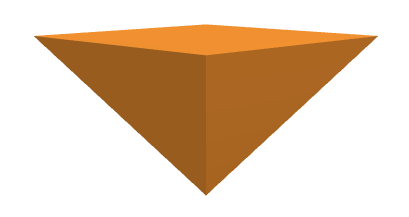
\includegraphics[width=0.25\columnwidth]{dojo/linearized_cone.png}
	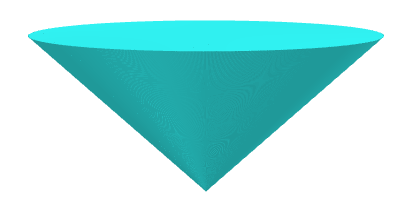
\includegraphics[width=0.25\columnwidth]{dojo/nonlinear_cone.png}
	\hfill
	\caption[Linearized and second-order friction-cone comparison]{Friction-cone comparison. Linearized double-parameterized (left) and nonlinear second-order (right) cones.}
	\label{intro_friction_cone_comparison}
\end{figure}
Coulomb friction \cite{moreau2011unilateral} models stick-slip behavior with friction that instantaneously maximizes the dissipation of kinetic energy between two objects in contact while remaining within a friction-cone. For a single contact point, this physical phenomenon can be modeled by the following optimization problem:
\begin{equation}
	\begin{array}{ll}
		\underset{b}{\mbox{minimize}} & \nu^T b\\
		\mbox{subject to} &\|b\|_2\leq \mu \gamma, \\
	\end{array} \label{intro_mdp}
\end{equation}
where $\nu \in \mathbf{R}^{2}$ is the tangential velocity at the contact point, $b \in \mathbf{R}^2$ is the friction force, and $\mu \in \mathbf{R}_{+}$ is the coefficient of friction between two objects \cite{moreau2011unilateral}. 

This problem is naturally a convex second-order cone program, and can be efficiently and reliably solved \cite{lobo1998applications}. However, classically, an approximate version of \eqref{intro_mdp}:
\begin{equation}
	\begin{array}{ll}
		\underset{\beta}{\mbox{minimize}} & \nu^T D^T \beta \\
		\mbox{subject to} & \beta^T \textbf{1} \leq \mu \gamma, \\
		& \beta \geq 0, \\
	\end{array} \label{intro_mdp_linear}
\end{equation}
formulated as a linear program, is instead solved. Here, the friction cone is linearized, (Fig. \ref{intro_friction_cone_comparison}) and the friction vector, $\beta \in \mathbf{R}^{2 d}$, is over parameterized and subject to additional non-negative constraints \cite{stewart1996implicit}, and $D \in \mathbf{R}^{2d \times 2}$ is the parameterization mapping. Finer discretization (i.e., larger $d$) of the friction cone can be utilized to better approximate the original problem, at the expense of a larger and computationally more expensive optimization problem.

The optimality conditions for \eqref{intro_mdp_linear} are:
\begin{align}
	\psi \cdot [\mu \gamma - \textbf{1}^T \beta] &= 0, \label{intro_friction_velocity_complementarity}\\
	\beta \circ [D \nu - \psi \textbf{1}] &= 0, \label{intro_friction_impulse_complementarity}\\
	\psi, \beta, [\mu \gamma - \textbf{1}^T \beta], [D \nu - \psi \textbf{1}] & \geq 0 \label{intro_friction_inequality}, 
\end{align}
where $\psi \in \mathbf{R}$ is a dual variable that can be interpreted as the magnitude of the contact-point tangential velocity, $\textbf{1}$ is a vector of ones, and $\circ$ is an element-wise product.

The primary drawback to this formulation is that the optimized friction force will naturally align with the vertices of the cone approximation, which may not align with the velocity vector of the contact point. This can lead to simulation artifacts such as creep. The reason this set of constraints is often preferred in practice is because they satisfy the requirements for a linear complementarity problem.

\paragraph{Linear complementarity problem.}
Contact dynamics are classically simulated with a velocity-based
time-stepping scheme formulated as a linear complementarity problem (LCP). This formulation combines the system's smooth dynamics with impact (\ref{intro_sdf}-\ref{intro_impact_complementarity}) and friction constraints (\ref{intro_friction_velocity_complementarity}-\ref{intro_friction_inequality}) in order to optimize the next velocity, $v \in \mathbf{R}^{n_v}$ of the system by finding the physically correct contact impulses, $\lambda = (\beta, \gamma)$. The next configuration $q \in \mathbf{R}^{n_q}$ is recovered from the solution: $q = q_{-} + h v$. Values at the previous time step are indicated with negative subscripts ($_{-}$). For a single contact point, dynamics are formulated as follows: 
\begin{align}
	\label{intro_feas_prob}
	{\mbox{find}} \quad & v, \lambda, \psi \\
	\mbox{subject to} \quad & M(q_{-}) (v - v_{-}) / h + C(q_{-}, v_{-}) = J(q_{-})^T \lambda, \notag \\
	& \gamma \circ [\phi(q_{-}) + \phi_q(q_{-}) \cdot h v] = 0, \notag\\
	& \psi \cdot \left[\mu \gamma - \textbf{1}^T \beta \right] = 0, \notag \\
	& \beta \circ [D J(q_{-}) v + \psi \textbf{1}] = 0, \notag\\
	& \phi, \gamma, [\mu \gamma - \textbf{1}^T \beta], [D J(q_{-}) v + \psi \textbf{1}], \beta, \psi \geq 0, \notag
\end{align}
where $M \in \mathbf{S}_{++}^{n_v}$ is the mass matrix, $C \in \mathbf{R}^{n_v}$ is the dynamics bias, $J \in \mathbf{R}^{(2d + 1) \times n_v}$ is the contact Jacobian that maps impulses at the contact point into the velocity space, and $h \in \mathbf{R}_{++}$ is the time step. The terms $M$, $C$, and $J$ are evaluated at the previous configuration, and a first-order approximation of the signed distance function at the previous configuration is utilized. This formulation generalizes to multiple contacts. 

Specialized solvers exist for LCPs. Typically, these optimizers rely on active-set methods that utilize pivoting algorithms to search the space of valid complementarity conditions \cite{dirkse1995path}.

\section{Contact-Implicit Trajectory Optimization}
Direct trajectory optimization can utilize the LCP contact dynamics formulation to plan trajectories for systems that make and break contact with their environment \cite{posa2014direct} without requiring hybrid dynamics \cite{westervelt2003hybrid} or explicitly enumerating all of the possible sequences of contact configurations. This enables the optimizer to potentially generate motion plans without pre-specified contact plans using task-level specifications via an objective.
 
\paragraph{Problem.} The contact-implicit trajectory optimization problem:
\begin{align}
	\underset{\substack{x_{1:T}, u_{1:T-1}, \\ \lambda_{1:T-1}, \psi_{1:T-1}}}{\mbox{minimize }} & c_T(x_T) + \sum \limits_{t = 1}^{T-1} c_t(x_t, u_t) \label{intro_ci_trajopt}\\
	\mbox{subject to} & \quad M(q_{t}) (v_{t+1} - v_{t}) / h + C(q_t, v_t) -B(q_{t}) u - J(q_{t})^T \lambda_t = 0, \quad t = 1,\dots,T-1, \notag \\
	& \quad q_t + h v_{t+1} - q_{t+1} = 0, \quad \quad \, \, \, \, \quad \quad \quad \quad \quad \quad \quad \quad \quad \quad \quad \quad \quad \, \, t = 1,\dots,T-1, \notag \\
	& \quad \gamma_t \circ \phi(q_{t+1}) = 0, \notag \quad \quad \quad \quad \, \, \, \, \, \, \, \quad \quad \quad \quad \quad \quad \quad \quad \quad \quad \quad \quad \quad \, \, t = 1,\dots,T-1, \notag\\
	& \quad \psi_t \cdot \left[\mu \gamma_t - \textbf{1}^T \beta_t \right] = 0, \, \, \,  \, \, \quad \quad \quad \quad \quad \quad \quad \quad \quad \quad \quad \quad \quad \quad \quad \, \, t = 1,\dots,T-1, \notag \\
	& \quad \beta_t \circ [D J(q_{t}) v_{t+1} + \psi_t \textbf{1}] = 0, \, \quad \quad \quad \quad \quad \quad \quad \quad \quad \quad \quad \quad \quad \, t = 1,\dots,T-1, \notag\\
	& \quad \phi(q_{t+1}), \gamma_t, [\mu \gamma_t - \textbf{1}^T \beta], [D J(q_{t}) v_{t+1} + \psi_t \textbf{1}], \beta_t, \psi_t \geq 0, \quad \quad t = 1,\dots,T-1, \notag \\
	& \quad (x_1 \, \mbox{given}) \notag,
\end{align}
with states, $x = (q, v)$, directly encodes the LCP constraints and aims to minimize an objective. This formulation generalizes to multiple contacts. 

\paragraph{Complementarity reformulation.} To work well in practice with general-purpose off-the-shelf solvers for non-convex problems, the complementarity constraints are reformulated using an exact $\ell_1\mbox{-norm}$ penalty \cite{manchester2020variational}:
\begin{equation}
	\begin{array}{ll}
		\underset{}{\mbox{find }}  & a, b\\
		\mbox{subject to } & a \circ b = 0, \\ 
		& a, b \geq 0
	\end{array}
	\quad
	\rightarrow 
	\quad
	\begin{array}{ll}
		\underset{a, b, s}{\mbox{minimize }}  & \rho s\\
		\mbox{subject to } & s \mathbf{1} - a \circ b \geq 0, \\
		& a, b, s \geq 0
	\end{array} \label{intro_complementarity_reformulation}
\end{equation}
This formulation relaxes the complementarity constraints and empirically results in superior convergence properties. As $\rho \rightarrow \infty$, we have $s \rightarrow 0$, and the original formulation is recovered. Despite the reformulation's practical performance, it requires additional decision variables and careful selection of the initial penalty parameter, $\rho \in \mathbf{R}_+$.

\section{Predictive Control}
A powerful tool for controlling complex systems is predictive control (PC) \cite{richalet1978model}. These algorithms leverage fast dynamics and planning algorithms to perform online optimization. This framework has been successfully deployed in numerous real-world settings including: control for chemical and nuclear processes \cite{na2003model, lopez2013fast}, navigation for autonomous vehicles \cite{falcone2007predictive}, and whole-body control of humanoid robots \cite{atlas2019parkour}.

In this framework, a model and the current state are utilized to predict the future evolution of the system under candidate action sequences. Numerical optimization is performed online to search for improved sequences. The best plan is utilized to control the system until a new (hopefully) improved plan has been computed.

\paragraph{Problem.}
The predictive control policy:
\begin{align}
	u \leftarrow \pi(x)
	\begin{cases}
		\begin{array}{ll}
			\underset{x_{1:T}, u_{1:T}}{\mbox{minimize }}  & \sum \limits_{t = 1}^{T} c_t(x_t, u_t) \\
			\mbox{subject to } & x_{t+1} = f_t(x_t, u_t),  \quad t = 1, \dots, T,\\
			& x_1 = x
		\end{array}
	\end{cases}
	\label{intro_mpc_policy}
\end{align}
is formulated as an optimization problem where $T$ is the planning horizon, typically much shorter than the horizon we care to control the system. The optimized action sequence is utilized to return an action from the policy. If replanning is performed at a high rate, the resulting sequence of open-loop plans will effectively perform feedback.

\paragraph{Practical enhancements.} There are three key enhancements for PC algorithms that lead to its practical performance. First, actions returned by the policy from approximate solutions to the internal optimization problem are often highly effective. As a result, since it is not necessary to solve the problem to convergence the computational burden is substantially reduced, enabling faster replanning, which typically leads to superior feedback. 

Second, myopic planning horizons are typically sufficient to achieve desired long-term behavior (i.e., minimizing total returns over the full planning horizon). This enables simpler models that may be easier to construct and less expensive to evaluate to be used during forward prediction since simulating accurate long-term behavior is not necessary. 

Third, the temporal nature of the control problem results in sequential policy evaluations that will solve similar optimization problems. As a result, warm starting, where the solution to a previous problem is used as a starting point for the current problem, can be effectively utilized. Employing this technique can greatly reduce the computational cost of policy evaluations.

\section{Augmented Lagrangian Method}
For equality-constrained problems, the augmented Lagrangian method \cite{bertsekas2014constrained} is a simple and effective algorithm, particularly when the problem is non-convex. This method transforms the constrained problem into an unconstrained form, then alternates between minimizing an augmented objective and performing updates to the dual variables and a penalty parameter.

\paragraph{Problem.}
An equality-constrained problem:
\begin{equation}
	\begin{array}{ll}
		\underset{x}{\mbox{minimize }}  & c(x) \\
		\mbox{subject to } & g(x) = 0, \\
	\end{array}
	\label{intro_equality_constrained}
\end{equation}
is transformed into an unconstrained problem by introducing dual variables, $\lambda \in \mathbf{R}^m$, and a quadratic penalty parameterized by $\rho \in \mathbf{R}_+$:
\begin{equation}
	L_{\mathcal{A}}(x; \lambda, \rho) = c(x) + \lambda^T g(x) + \frac{\rho}{2} g(x)^T g(x), 
	\label{intro_augmented_lagrangian}
\end{equation}
where we refer to $L_{\mathcal{A}}$ as the \emph{augmented Lagrangian} for the problem \eqref{intro_equality_constrained}.

\paragraph{Primal method.}
The classic method alternates between minimizing the augmented Lagrangian  \eqref{intro_augmented_lagrangian} and performing outer updates on the dual variables and penalty:
\begin{equation} 
	\lambda \leftarrow \lambda + \rho g(x), \quad \rho \leftarrow \phi (\rho), \label{intro_augmented_lagrangian_update}
\end{equation}
until a solution to the original problem \eqref{intro_equality_constrained} is found \cite{bertsekas2014constrained}. This typically requires ten or fewer outer updates and a simple update, $\phi : \mathbf{R}_+ \rightarrow \mathbf{R}_+$, that scales the penalty by a constant value, works well in practice.
Throughout, subscripts are used to denote derivatives and we drop the variable dependence of the functions for clarity. The KKT system for this method is:
\begin{equation} 
	\Big[c_{xx} + \rho g_x^T g_x + \sum \limits_{i = 1}^m (\lambda^{(i)} + \rho g^{(i)}) g_{xx}^{(i)} \Big] \Delta x = -\Big[c_x + g_x^T (\lambda + \rho g)\Big]. \label{intro_augmented_lagrangian_update} 
\end{equation}

Search directions $\Delta x \in \mathbf{R}^n$ are computed by solving the linear system \eqref{intro_augmented_lagrangian_update} for fixed values of the dual variables and penalty. Newton's method with a line search is utilized to compute iterates that satisfy the KKT conditions, or residual, to a desired tolerance.

While this simple algorithm is effective at finding low to medium quality solutions, the KKT matrix becomes increasingly ill-conditioned as the penalty is increased in order to achieve better satisfaction of the equality constraints, degrading the quality of the Newton step. As a result, this method is best suited for applications where finding approximate solutions quickly is desirable, but highly accurate solutions are unnecessary.

\paragraph{Primal-dual method.}
To address the deficiencies of the primal method, a primal-dual method introduces additional dual variables, $y \in \mathbf{R}^m$, and constraints:
\begin{equation}
	y = \lambda + \rho g(x), \label{intro_dual_constraint}
\end{equation}
in order to utilize an alternative KKT system with better numerical properties.

Combining these constraints \eqref{intro_dual_constraint} with the primal KKT system \eqref{intro_augmented_lagrangian_update} and performing a simple manipulation of the new equations yields 
the \textit{primal-dual} augmented-Lagrangian KKT system:
\begin{align}
	\setstackgap{L}{1.1\baselineskip}
	% \fixTABwidth{T}
	\bracketMatrixstack{
		c_{xx} + \sum \limits_{i = 1}^m y^{(i)} g_{xx}^{(i)} & g_x^T \\ 
		g_x & -\frac{1}{\rho} I
	}
	\bracketVectorstack{ 
		\Delta x \\ 
		\Delta y
	}
	= 
	-\bracketMatrixstack{ 
		c_x + g_x^T y \\ 
		g + \frac{1}{\rho}(\lambda - y) 
	}. \label{intro_augmented_lagrangian_primal_dual}
\end{align}
In contrast to the primal system \eqref{intro_augmented_lagrangian_update}, this system \eqref{intro_augmented_lagrangian_primal_dual} does not become ill-conditioned as the penalty is increased because this term does not appear in the KKT matrix---only its inverse appears (i.e., $-\frac{1}{\rho} I$), which actually enhances the conditioning of the system by performing dual regularization  \cite{kuhlmann2018primal,gill2012primal,argaez2002global}. Further, this method implicitly satisfies the linear independence constraint qualification (LICQ) \cite{nocedal2006numerical}, necessary for most second-order methods for constrained optimization, because the KKT matrix remains full rank even in cases where $g_x$ is rank deficient as a result of the dual regularization \cite{izmailov2012global}.

Additionally, the KKT conditions now contain relaxed constraints (i.e., $g(x) + \frac{1}{\rho}(\lambda - y))$ that are particularly helpful for complementarity constraints since these elements of the residual are only satisfied in the limit as outer updates are performed.

Similar to the primal method, search directions ($\Delta x, \Delta y$) are computed by solving the linear system \eqref{intro_augmented_lagrangian_primal_dual} for fixed values of the dual variables estimates and penalty. Newton's method with a line search is utilized to compute iterates that satisfy the KKT conditions, or residual, to a desired tolerance. Outer updates to the dual estimates and penalty parameter are performed as before.

\section{Interior-Point Method}
For problems with hundreds to tens of thousands of decision variables and cone constraints, interior-point methods are efficient and return highly accurate solutions.
\paragraph{Problem.}
A cone program:
\begin{equation}
	\begin{array}{ll}
		\underset{x}{\mbox{minimize }}  & c(x) \\
		\mbox{subject to } & x \in \mathcal{K}, \\
	\end{array}
	\label{intro_cone_program}
\end{equation}
minimizes an objective while satisfying a cone constraint. For robotics applications, common cones include the positive orthant (i.e., inequality constraints):
\begin{equation} 
	x^{(i)} \ge 0, \quad i = 1, \dots, n \quad \rightarrow \quad x \in \mathbf{R}^n_{+},
\end{equation}
and second-order cones:
\begin{equation}
	\|x^{(2:n)}\|_2 \leq x^{(1)} \quad \rightarrow \quad x \in \mathcal{Q}^n.
\end{equation}

\paragraph{Primal method.}
An interior-point method transforms the original constrained problem  \eqref{intro_cone_program} into an unconstrained form using a logarithmic barrier:
\begin{equation}
	L_{\mathcal{B}}(x; \kappa) = c(x) - \kappa \phi(x),
	\label{intro_barrier_function}
\end{equation}
where we refer to $L_{\mathcal{B}}$ as the \textit{barrier Lagrangian}. The barrier functions are:
\begin{equation}
	\phi(x) = \sum \limits_{i = 1}^n \mbox{log}(x^{(i)}),
\end{equation}
and 
\begin{equation}
	\phi(x) = \frac{1}{2} \mbox{log}\Big((x^{(1)})^2 - (x^{(2:n)})^T x^{(2:n)} \Big),
\end{equation}
for the positive orthant and second-order cone, respectively.

The classic method alternates between minimizing the barrier Lagrangian \eqref{intro_barrier_function} while taking steps that ensure the cone constraint remains satisfied, and outer updates to the central-path parameter, $\kappa \in \mathbf{R}_{+}$, until a solution to the original problem \eqref{intro_cone_program} is found \cite{boyd2004convex}. An effective strategy for the update is to decrease the parameter by a constant factor, $\kappa \rightarrow 0$. 

The KKT system for this method is:
\begin{equation}
	\Big[c_{xx} - \kappa \phi_{xx} \Big] \Delta x = -\Big[c_x - \kappa \phi_x \Big]. \label{intro_barrier_gradient}
\end{equation}
As the central-path parameter is decreased, the logarithmic barrier becomes a closer approximation to the indicator function, which has an infinite cost if a constraint is violated and is otherwise zero \cite{boyd2004convex}. While simple, this approach suffers from numerical ill-conditioning, similar to the primal augmented Lagrangian method, as the central-path parameter approaches zero, degrading a solver's ability to find accurate solutions to the original problem \eqref{intro_cone_program}.

\paragraph{Primal-dual method.} 
To address the conditioning issues of the primal method, additional dual variables, $z \in \mathbf{R}^n$, and complementarity constraints are introduced to form a new KKT system:
\begin{align} 
	\setstackgap{L}{1.25\baselineskip}
	\begin{bmatrix} 
		c_{xx} & -I \\ 
		\mbox{\textbf{diag}}(z)  & \mbox{\textbf{diag}}(x) 
	\end{bmatrix}
	\begin{bmatrix} 
		\Delta x \\ 
		\Delta z
	\end{bmatrix} &= 
	-
	\bracketMatrixstack{ 
		c_x - z \\
		x \circ z - \kappa \mathbf{e}
	}, \label{intro_interior_point_primal_dual}\\
	x \in \mathcal{K}, z &\in \mathcal{K}^* \label{intro_cone_primal_dual_cones}.
\end{align}
Similar to the primal-dual augmented Lagrangian method, this KKT matrix does not depend on the central-path parameter, resulting in significantly better numerical conditioning than primal methods. The complementarity constraints in the KKT conditions are relaxed (i.e., $x \circ z - \kappa \mathbf{e})$, only being satisfied in the limit as the central-path parameter is decreased to zero. For the positive orthant, the target $\mathbf{e} = \mathbf{1}$ and the cone product $\circ$ denotes an element-wise product. For the second-order cone, the target is: $\mathbf{e} = (1, 0^{(n-1)})$, with cone product: $a \circ b = (a^T b, \, a^{(1)} b^{(2:n)} + b^{(1)} a^{(2:n)})$ \cite{domahidi2013ecos, vandenberghe2010cvxopt}. Both cones are self dual \cite{boyd2004convex}, and $\mathcal{K} = \mathcal{K}^*$.

With the new system, search directions ($\Delta x, \Delta z$) are computed by solving the linear system \eqref{intro_interior_point_primal_dual} for fixed values of the central path parameter. Newton's method with a line search is utilized to compute iterates that satisfy the KKT conditions, or residual, to a desired tolerance, while respecting the cone constraints on the primal and dual variables. Updates to the central-path parameter are performed as before.

\section{Implicit Differentiation}
Many optimization problems can be formulated as finding a fixed point to an implicit function. An implicit function, $r : \mathbf{R}^a \times \mathbf{R}^b \rightarrow \mathbf{R}^a$, is defined as:
\begin{equation}
	r(w^*; \theta) = 0, \label{intro_implicit_function}
\end{equation}
for a fixed-point $w^* \in \mathbf{R}^a$ and problem data $\theta \in \mathbf{R}^b$. Further, it is often useful to compute the sensitivity of this solution with respect to the problem data, i.e., differentiate through the implicit function.

Computing this sensitivity is possible by applying the implicit-function theorem \cite{dini1907lezioni}. First, the function is approximated to first order at the solution:
\begin{equation}
	\cancelto{0}{r} + \frac{\partial r}{\partial w} \delta w + \frac{\partial r}{\partial \theta} \delta \theta = 0.
\end{equation}
Then, it is possible to solve for the relationship: 
\begin{equation}
	\frac{\partial w^*}{\partial \theta} = -\Big(\frac{\partial r}{\partial w}\Big)^{-1} \frac{\partial r}{\partial \theta}, \label{intro_solution_sensitivity}
\end{equation}
and recover the sensitivity.

Newton's method is typically employed to find solutions. When the method succeeds, the sensitivity \eqref{intro_solution_sensitivity} can be computed and the factorization of $\partial r / \partial w$ used to find the solution is reused to efficiently compute sensitivities at very low computational cost, using only back-substitution. In the case that $\partial r / \partial w$ is not full rank, an approximate solution, e.g., least-squares \cite{boyd2004convex}, can be computed, or regularization can be employed. Additionally, each element of the sensitivity can be computed in parallel.

\paragraph{Differentiating through an optimization problem.}
Implicit differentiation can also be used to compute the sensitivity of solutions, found by numerical optimizers, with respect to the optimization problem data. Numerical solvers find fixed points, comprising primal and dual variables, to the gradient of the problem's Lagrangian. This approach has been successfully applied to quadratic programs \cite{amos2017optnet}, and more generally, convex cone programs \cite{agrawal2019differentiating}.

While it is possible to compute derivatives via finite-difference schemes, this approach requires at least as many calls to the solver as there are problem data elements. An alternative approach to computing gradients through a solver is to unroll the algorithm and utilizing the chain rule to differentiate sequentially through each iteration \cite{domke2012generic}. However, in practice, this approach requires truncating the number of iterates, which can lead to low-accuracy solutions, and this approach can be plagued by numerical issues that lead to exploding or vanishing gradients. Implicit differentiation is generally more efficient and able to return highly accurate sensitivities. 





\chapter{Differentiable Contact Dynamics}

We present Dojo, a differentiable physics engine for robotics that prioritizes stable simulation, accurate contact physics, and differentiability with respect to states, actions, and system parameters. Dojo achieves stable simulation at low sample rates and conserves energy and momentum by employing a variational integrator. A nonlinear complementarity problem, with second-order cones for friction, models hard contact and is reliably solved using a custom primal-dual interior-point method. Special properties of the interior-point method are exploited using implicit differentiation to efficiently compute smooth gradients that provide useful information through contact events. We demonstrate Dojo's unique ability to simulate hard contact while providing smooth, analytic gradients with a number of examples, including trajectory optimization, policy optimization, and system identification.

\vspace*{\fill}

\noindent Dojo: A Differentiable Physics Engine for Robotics. Taylor A. Howell$^*$, Simon Le Cleac'h$^*$, Zico Kolter, Mac Schwager, and Zachary Manchester. arXiv 2203.00806. 2022.

\pagebreak

\section{Introduction}
The last decade has seen immense resources devoted to network architectures, optimization algorithms, and the construction of large datasets by the learning community. These efforts have been leveraged to make impressive advances in robotics including: dexterous manipulation \cite{andrychowicz2020learning,akkaya2019solving}, quadrupedal locomotion \cite{lee2020learning, kumar2021rma}, and pixels-to-torques control \cite{levine2018learning}. In contrast, there has been comparatively little work on the lowest level of the robotics stack: the \textit{physics engine}. We argue that deficiencies in current widely used physics engines form a key bottleneck that must be overcome to enable future advancements in robotics. 

Physics engines that simulate rigid-body dynamics with contact are utilized for trajectory optimization, reinforcement learning, system identification, and dataset generation for domains ranging from locomotion to manipulation. To be of practical value in real-world applications and overcome the sim-to-real gap an engine should provide stable simulation, accurately emulate a robot's dynamics, and ideally, be differentiable to enable use of efficient gradient-based optimization methods.

In recent years, a number of physics engines \cite{drake, freeman2021brax, werling2021fast, geilinger2020add, hu2019difftaichi, heiden2020neuralsim} have been developed and utilized for robotics. In this work, we address key deficiencies of these tools including: high sample rates required for stable simulation that exacerbate the vanishing/exploding gradient problem and substantially increase sample complexities for rollout-based optimization methods, interpenetration of rigid bodies (e.g., a robot foot sinking through the floor) or creep (e.g., objects that should be at rest incorrectly sliding), and lack of informative gradients  through contact events (e.g., subgradients resulting from naïve differentiation of non-smooth dynamics) or expensive gradients that require a large number of calls to the engine (e.g., finite-difference or stochastic-sampling schemes).

The Dojo physics engine is designed from the ground up to enable better and easier optimization for motion planning, control, reinforcement learning, system identification, and high-quality dataset generation. By taking a physics- and optimization-first approach to physics-engine design, we significantly advance the state of the art in \textit{stable simulation}, \textit{accurate contact physics}, and \textit{differentiability} for robot simulation. Key attributes of Dojo include: 
\begin{itemize}
	\item Variational integration for stable simulation that is not sensitive to time step size
	\item A nonlinear complementarity problem (NCP) model for accurate contact dynamics
	\item A custom primal-dual interior-point method for reliably solving the NCP 
	\item Smooth, analytic gradients that provide useful information through contact events
\end{itemize}

In the remainder of this chapter, we first provide an overview of related state-of-the-art physics engines in Section \ref{dojo_related_work}. Next, we present Dojo, and its key features, in Section \ref{dojo}. Simulation, planning, policy optimization, and system identification examples are presented in Section \ref{dojo_results}. Finally, we discuss Dojo's limitations in Section \ref{dojo_limitations} and provide closing remarks in Section \ref{dojo_future_work}.

\section{Related Work} \label{dojo_related_work}

This section provides an overview of physics engines that are commonly used in robotics. Table \ref{dojo_engine_comparison} summarizes the features of these tools and compares them to Dojo.

Many physics engines being developed and used in practice today were not designed for real-world robotics applications, and it is common for these tools to prioritize the \textit{appearance} of realism over actual physical accuracy. Additionally, many of these physics engines were designed primarily for graphics and animation applications where fast simulation rates are prioritized and general-purpose numerical-optimization routines that do not natively support key elements from robotics domains, like cone constraints or quaternions, are commonplace. In this section, we provide background on a collection of popular engines, including: discussion of physical fidelity, underlying optimization routines, and ability to return gradients.

In the learning community, \emph{MuJoCo}~\cite{todorov2012mujoco} has become a standard for benchmarking reinforcement learning algorithms using the OpenAI Gym environments~\cite{brockman2016openai}.
MuJoCo utilizes minimal-coordinates representations and employs both semi-implicit Euler and explicit fourth-order Runge-Kutta integrators to simulate multi-body systems. These integrators often require small time steps, particularly for systems experiencing contact, and typically sample rates of hundreds to thousands of Hertz are required for stable simulation, which a mature and efficient implementation is able to achieve much faster than real-time rates. However, the high simulation rates can prove a challenge for control tasks like reinforcement learning settings where vanishing or exploding gradients are exacerbated over long horizons with many time steps.

Impact and friction are modeled using a smooth, convex contact model \cite{todorov2014convex}. While this approach reliably computes contact forces, it introduces artificial damping, allowing the system to experience unphysical interpenetration and forces at a distance (i.e., while not in contact) and the default friction model introduces additional artifacts like velocity drift during sliding. Additionally, achieving good simulation behavior often requires system-specific tuning of multiple solver parameters. Further, the ``soft" contact model is computed using a \textit{primal} optimization method, meaning that as parameters are set to produce ``hard,'' or more realistic contact, the underlying optimization problem becomes increasingly ill-conditioned and difficult to solve. As a result, it is often not possible to eliminate unphysical artifacts from the simulation and produce realistic results. Finally, analytical gradients are not provided by the engine, requiring finite-difference schemes.

\emph{Drake \cite{drake}} was designed for robotics applications and its contact dynamics primarily rely on the classic time-stepping contact model that solves a linear complementarity problem (LCP) at each time step \cite{stewart1996implicit}. To satisfy the LCP problem formulation, a number of approximations are made to the dynamics and contact model, including the use of an approximate friction cone. To ensure stability of the simulation, small time steps are used where linearizations of the dynamics are valid, but importantly, the engine can achieve accurate hard contact. General-purpose LCP solvers that are typically used rely on a pivoting method like Lemke's algorithm \cite{cottle2009linear}. Randomized smoothing has been proposed as a method for returning gradients through contact \cite{suh2022bundled} with this model. Higher-fidelity models are available for patch contacts \cite{elandt2019pressure}, but they are computationally more expensive, requiring sophisticated higher-order implicit integrators.

The popular robotics simulator \emph{Gazebo} \cite{koenig2004design} can utilize several different physics engines to simulate multi-body contact dynamics; Bullet \cite{heiden2020neuralsim} and DART \cite{lee2018dart} are common choices. Similar to Drake, these engines model hard contact dynamics with a LCP formulation. Automatic differentiation tools have also been utilized to compute gradients \cite{heiden2020neuralsim}. However, because of the discontinuous nature of contact dynamics, this approach will sometimes return sub-gradients, which do not provide useful information through contact events. Heuristics have been proposed to enumerate contact modes in order to select informative sub-gradients \cite{werling2021fast}. However, this approach scales poorly with the number of mode switches.

Engines designed for hardware accelerators (e.g., GPUs), including \emph{Brax} \cite{freeman2021brax} and \emph{PhysX} \cite{physx2022engine}, utilize simplified contact models that are amenable to low-precision data types (e.g., Float32). The benefit is massive parallel computation. However, these engines often require system-specific tuning to achieve stable simulation and the results are typically lower-fidelity.

Building on previous work \cite{brudigam2021linear}, Dojo utilizes the open-source maximal-coordinates dynamics library \texttt{ConstrainedDynamics.jl} and efficient graph-based linear-system solver \texttt{GraphBasedSystems.jl} to compute smooth dynamics. However, unlike this prior work, Dojo has an improved contact model, specifically with regard to friction and its representation in the graph structure. Additionally, Dojo implements an efficient and reliable differentiable interior-point solver for complementarity problems.

The properties and characteristics of these existing engines are summarized in Table \ref{dojo_engine_comparison}. We find that none of the existing engines prioritize two of the most important attributes for robotics: physical accuracy and useful differentiability. This motivates our development of a new physics engine for robotics applications.

\begin{table}[H]
	\centering
	\caption[Comparison of physics engines used for robotics]{Comparison of physics engines used for robotics.}
	\small
	\begin{tabular}{c c c c c c c}
		\toprule
		\textbf{Engine} & \textbf{Integrator} & \textbf{State} & \textbf{Contact} & \textbf{Solver} & \textbf{Gradients} \\
		\toprule
		MuJoCo \cite{todorov2012mujoco} & RK4 & minimal & soft & Newton & finite-difference \\
		Drake \cite{drake} & implicit Euler & minimal & soft/hard & LCP & randomized-smoothing\\
		Bullet \cite{coumans2019} & implicit Euler & minimal & soft/hard & LCP & sub-gradient \\
		DART \cite{lee2018dart} & implicit Euler & minimal & hard & LCP & sub-gradient\\
		PhysX \cite{physx2022engine} & explicit & minimal & soft & iterative & finite-difference \\
		Brax \cite{freeman2021brax} & explicit & maximal & soft & iterative & sub-gradient\\
		\hline
		\textbf{Dojo} & variational & maximal & hard & NCP & implicit gradient \\
		\toprule
	\end{tabular}
	\label{dojo_engine_comparison}
\end{table}
%===============================================================================

\section{Dojo} \label{dojo}

We now introduce Dojo's contact dynamics model and custom interior-point solver. This section presents the key algorithms and subroutines, including: variational integrators, the contact model, a differentiable primal-dual interior-point solver, and the computation of smooth gradients. An open-source implementation of the engine is provided.

\subsection{Maximal-coordinates representation} 
Most multi-body physics engines utilize minimal- or joint-coordinates representations for dynamics because of the small number of states and convenience of implementation. This results in small, but dense systems of linear equations. In contrast, maximal-coordinates explicitly represent the position, orientation, and velocities of each body in a multi-body system. This produces large, sparse systems of linear equations that can be efficiently solved, including in the contact setting. We provide an overview, largely based on prior work \cite{brudigam2020linear}, of this representation. 

A single rigid body is defined by its mass and inertia, and has a configuration, $x = (p, q) \in \mathbf{X} = \mathbf{R}^3 \times \mathbf{H}$, comprising a position $p$ and unit quaternion $q$, where $\mathbf{H}$ is the space of four-dimensional unit quaternions. We define the implicit discrete-time dynamics $F : \mathbf{X} \times \mathbf{X} \times \mathbf{X} \rightarrow \mathbf{R}^{6}$ as: 
\begin{equation}
	F(x_{-}, x, x_{+}) = 0, \label{dojo_implicit_dynamics}
\end{equation}
where we indicate the previous and next time steps with minus ($-$) and plus ($+$) subscripts, respectively, and the current time step without decoration.
A variational integrator is employed to simulate the next state of the system and has desirable energy and momentum conservation properties \cite{marsden2001discrete}. Linear and angular velocities are handled implicitly via finite-difference approximations.

For a multi-body system with bodies $a$ and $b$ connected via a joint---common types include: revolute, prismatic, and spherical---we introduce a constraint, $k : \mathbf{X} \times \mathbf{X} \rightarrow \mathbf{R}^{l}$, that couples the two bodies: 
\begin{equation} 
	k^{ab}(x^{a}_{+}, x^{b}_{+}) = 0. 
\end{equation} 
An impulse, $j \in \mathbf{R}^l$, where $l$ is equal to the six degrees-of-freedom of an unconstrained body minus the joint's number of degrees-of-freedom, acts on both bodies to satisfy the constraint. The implicit integrator for the multi-body system has the form,
\begin{equation} 
	\begin{bmatrix} 
		F^{a}(x^{a}_{-}, x^{a}, x^{a}_{+}) + K^{a}(x^{a}, x^{b})^T j^{ab} \\ 
		F^{b}(x^{b}_{-}, x^{b}, x^{b}_{+}) + K^{b}(x^{a}, x^{b})^T j^{ab} \\ 
		k^{ab}(x^{a}_{+}, x^{b}_{+})
	\end{bmatrix} = 0, \label{dojo_max_2body}
\end{equation}
where $K: \mathbf{X} \times \mathbf{X} \rightarrow \mathbf{R}^{l \times 6}$ is a mapping from the joint to the maximal-coordinates space and is related to the Jacobian of the joint constraint.

We can generalize  \eqref{dojo_max_2body} to include additional bodies and joints. For a system with $N$ bodies and $M$ joints we define a maximal-coordinates configuration $z = (x^{(1)}, \dots, x^{(N)}) \in \mathbf{Z}$ and joint impulse $j = (j^{(1)}, \dots, j^{(M)}) \in \mathbf{J}$. We define the implicit discrete-time dynamics of the maximal-coordinates system as: 
\begin{equation} 
	F(z_{-}, z, z_{+}, j) = 0, \label{dojo_max_implicit_dynamics}
\end{equation}
where $F: \mathbf{Z} \times \mathbf{Z} \times \mathbf{Z} \times \mathbf{J} \rightarrow \mathbf{R}^{6N}$. In order to simulate the system we find $z_{+}$ and $j$ that satisfy \eqref{dojo_max_implicit_dynamics} for a provided $z_{-}$ and $z$ using Newton's method. 

By exploiting the mechanism's structure, we can efficiently perform root finding on \eqref{dojo_max_implicit_dynamics} (see \cite{brudigam2020linear} for additional details). This structure is manifest as a graph of the mechanism, where each body and joint is considered a node, and joints have edges connecting bodies (Fig. \ref{dojo_graph_structure}). Because the mechanism structure is known \textit{a priori}, a permutation matrix can be precomputed and used to perform efficient sparse linear algebra during simulation. For instance, in the case where the joint constraints form a system without loops, the resulting sparse system can be solved in linear time with respect to the number of links.

\begin{figure}[H]
	\centering
	\includegraphics[width=0.75\columnwidth]{dojo/graph.tikz}
	\caption[Graph structure for maximal-coordinates state representation]{Graph structure for maximal-coordinates system with 4 bodies, 3 joints, and 3 points of contact.}
	\label{dojo_graph_structure}
\end{figure}

\subsection{Variational integrator}
We use a specialized implicit integrator that preserves energy and momentum, natively handles quaternions, and alleviates spurious artifacts that commonly arise from contact interactions. 

Dojo utilizes a maximal-coordinates state representation \cite{brudigam2020linear}. Each body has linear:
\begin{equation} 
	m (p_{+} - 2 p + p_{-}) / h - h m g - A(p)^T j - h f = 0, \label{dojo_linear_integrator}
\end{equation}
and rotational: 
\begin{equation}
	\sqrt{1 - \psi_+^T \psi_+} J \psi_+ + \psi_+ \times J \psi_+ - \sqrt{1 - \psi^T \psi} J \psi + \psi \times J \psi - B(q)^T j - h^2 \tau / 2 = 0,
	\label{dojo_rotational_integrator}
\end{equation}
dynamics specified by mass $m \in \mathbf{R}_{++}$, inertia $J \in \mathbf{S}_{++}^3$, gravity $g \in \mathbf{R}^3$, and time step $h \in \mathbf{R}_{++}$. Equations (\ref{dojo_linear_integrator}, \ref{dojo_rotational_integrator}) are essentially second-order centered-finite-difference approximations of Newton's second law and Euler's equation for the rotational dynamics where $q_+ = q \cdot (\sqrt{1 - \psi_+^T \psi_+}, \psi_+)$ is recovered from a three-parameter representation $\psi \in \mathbf{R}^3$ \cite{manchester2016quaternion}, respectively. Joint impulses $j \in \mathbf{J}$ have linear $A : \mathbf{R}^3 \rightarrow \mathbf{R}^{\mbox{dim}(\mathbf{J}) \times 3}$ and rotational $B : \mathbf{H} \rightarrow \mathbf{R}^{\mbox{dim}(\mathbf{J}) \times 3}$ mappings into the dynamics. The configuration of a body $z^{(i)} = (p^{(i)}, q^{(i)}) \in \mathbf{R}^3 \times \mathbf{H}$ comprises a position and orientation represented as a quaternion. Forces and torques $f, \tau \in \mathbf{R}^3$ can be applied to the bodies.

Both \eqref{dojo_linear_integrator} and \eqref{dojo_rotational_integrator} are derived by approximating Hamilton's Principle of Least-Action using a simple midpoint scheme \cite{marsden2001discrete,manchester2020variational}. This approach produces \emph{variational} integrators that automatically conserve momentum and energy \cite{marsden2001discrete}.

\subsection{Rigid-body dynamics with contact}
Impact and friction behaviors are modeled, along with the system's dynamics, as a complementarity problem. This model simulates hard contact without requiring system-specific solver tuning. Additionally, contacts between a system and the environment are treated as a single graph node connected to a rigid body (Fig \ref{dojo_graph_structure}). As a result, the engine retains efficient linear-time complexity for open-chain mechanical systems.

Dojo uses the classic impact model (\ref{intro_sdf}-\ref{intro_impact_inequality}) and in the following section we present a Coulomb friction model that utilizes an exact nonlinear friction cone.

\paragraph{Second-order friction cone.}
In contrast to the LCP formulation, we utilize the optimality conditions of \eqref{intro_mdp} in a form amenable to a primal-dual interior-point solver. The associated cone program is,
\begin{equation}
	\begin{array}{ll}
		\underset{\beta}{\mbox{minimize}} & v^T \beta_{(2:3)}\\
		\mbox{subject to} & \beta_{(1)} = \mu \gamma, \\
		& \|\beta_{(2:3)}\|_2 \leq \beta_{(1)},\\
	\end{array} \label{dojo_mdp_socp}
\end{equation}
where subscripts indicate vector indices.
The relaxed optimality conditions for (\ref{dojo_mdp_socp}) in interior-point form are: 
\begin{align}
	v - \eta_{(2:3)} &= 0, \\
	\beta_{(1)} - \mu \gamma &= 0, \\
	\beta \circ \eta &=  \kappa \mathbf{e}, \\
	\|\beta_{(2:3)}\|_2 \leq \beta_{(1)}, \, \|\eta_{(2:3)}\|_2 &\leq \eta_{(1)}, 
	\label{socp_mdp_constraints}
\end{align}
with dual variable $\eta \in \mathbf{R}^3$ associated with the second-order-cone constraints, and central-path parameter, $\kappa \in \mathbf{R}_{+}$. The benefits of this model are increased physical fidelity and fewer optimization variables, without substantial increase in computational cost.

\paragraph{Complementarity problem.}
Rigid-body dynamics with a single contact (this formulation extends to multiple contacts) is simulated using a time-stepping scheme that solves the feasibility problem,
\begin{align}
	\label{dojo_ncp}
	{\mbox{find}} \quad & z_{+}, j, \gamma, \beta, \eta\\
	\mbox{subject to} \quad & F(z_{-}, z, z_{+}, j, \lambda, u) = 0, \notag \\
	& v_c(z, z_{+}) - \eta_{(2:3)} = 0, \notag \\
	& \beta_{(1)} - \mu \gamma = 0, \notag\\
	& \gamma \cdot \phi(z_{+}) = \kappa, \notag \\
	& \beta \circ \eta = \kappa \mathbf{e}, \notag \\
	& \gamma, \phi(z_{+}) \geq 0, \, \|\beta_{(2:3)}\|_2 \leq \beta_{(1)}, \, \|\eta_{(2:3)}\|_2 \leq \eta_{(1)}, \notag
\end{align}
with actions $u = (f^{(1)}, \tau^{(1)}, \dots, f^{(N)}, \tau^{(N)}) \in \mathbf{U}$, and contact impulses $\lambda = (\beta_{(2:3)}, \gamma) \in \mathbf{\Lambda}$. The system's smooth dynamics $F : \mathbf{Z} \times \mathbf{Z} \times \mathbf{Z} \times \mathbf{J} \times \mathbf{\Lambda} \times \mathbf{U} \rightarrow \mathbf{R}^{6N}$ comprise linear and rotational dynamics (\ref{dojo_linear_integrator}-\ref{dojo_rotational_integrator}) for each body \cite{brudigam2020linear}. The central-path parameter $\kappa \in \mathbf{R}_{+}$ and target $\mathbf{e}$ \cite{vandenberghe2010cvxopt} are utilized by the interior-point solver in the following section. 

Solving the feasibility problem finds a maximal-coordinates state representation. In many applications it is desirable to utilize a minimal-coordinates representation (e.g., direct trajectory optimization where algorithm complexity scales with the state dimension). Dojo includes functionality to analytically convert between representations, as well as formulate and apply the appropriate chain rule in order to differentiate through a representation transformation.

To simulate a system forward in time one step, given a control input and state comprising the previous and current configurations, solutions to a sequence of barriers problems \eqref{dojo_ncp} are found with $\kappa \rightarrow 0$. The central-path parameter has a physical interpretation as being the softness of the contact model. A value $\kappa = 0$ corresponds to exact ``hard" or inelastic contact, whereas a relaxed value produces soft contact where contact forces can occur at a distance. The primal-dual interior-point solver described in the next section adaptively decreases this parameter in order to efficiently and reliably converge to hard contact solutions. In practice, the engine is set to converge to small values for simulation in order to simulate accurate physics. Intermediate solutions (i.e., $\kappa \neq 0$) are cached and later utilized to compute smooth gradients in order to provide useful information through contact events.

\subsection{Solver} 

To efficiently and reliably satisfy \eqref{dojo_ncp}, we developed a custom primal-dual interior-point solver for NCPs with support for cone constraints and quaternions. The algorithm is largely based upon Mehrotra's predictor-corrector algorithm \cite{mehrotra1992implementation, nocedal2006numerical}, while implementing non-Euclidean optimization techniques to handle quaternions \cite{jackson2021planning} and borrowing features from CVXOPT \cite{vandenberghe2010cvxopt} to handle cones. 

The primary advantages of this algorithm are the correction to the classic Newton step, which can greatly reduce the iterations required by the solver (often halving the total number of iterations), and feedback on the problem's central-path parameter that helps avoid premature ill-conditioning and adaptively drives the complementarity violation to zero in order to reliably simulate hard contact.

\paragraph{Problem.}
The solver aims to satisfy instantiations of the following problem:
\begin{equation}
	\begin{array}{ll}
		\underset{}{\mbox{find}} & a, b, c \\
		\mbox{subject to} & E(a, b, c; \theta) = 0, \\
		& b \circ c = \kappa \mathbf{e}, \\
		& b, c \in \mathcal{K},
	\end{array} \label{dojo_ncp_abstract}
\end{equation}
with decision variables $a \in \mathbf{R}^{n_{a}}$ and $b, c \in \mathbf{R}^{n_{b}}$, equality-constraint set $E : \mathbf{R}^{n_{a}} \times \mathbf{R}^{n_{b}} \times \mathbf{R}^{n_{b}} \times \mathbf{R}^{n_{\theta}} \rightarrow \mathbf{R}^{n_a + n_{b}}$, problem data $\theta \in \mathbf{R}^{n_{\theta}}$; and where $\mathcal{K}$ is the Cartesian product of positive-orthant and second-order cones \cite{boyd2004convex}. 

Interior-point methods aim to satisfy a sequence of relaxed problems with $\kappa > 0$ and $\kappa \rightarrow 0$ in order to reliably converge to a solution of the original problem (i.e., $\kappa = 0$). This continuation approach helps avoid premature ill-conditioning and is the basis for numerous convex and non-convex interior-point solvers \cite{nocedal2006numerical}.

The LCP formulation is a special-case instantiation \eqref{dojo_ncp_abstract} where the constraint set is affine in the decision variables, the cone is the positive orthant. Most general-purpose solvers for LCPs rely on active-set methods that strictly enforce $\kappa = 0$ at each iteration.

\paragraph{Residual and Jacobians.}
The interior-point solver aims to find a fixed point for the residual:
\begin{align}
	r(w; \theta, \kappa) &= \begin{bmatrix}
		E(w;\theta) \\
		b^{(1)} \circ c^{(1)} - \kappa \mathbf{1}\\
		\vdots \\
		b^{(n_{\mathcal{K}})} \circ c^{(n_{\mathcal{K}})} - \kappa \mathbf{e}\\
	\end{bmatrix}, \label{dojo_residual}
\end{align}
while respecting the cone constraints.
The Jacobian of this residual with respect to the decision variables,
\begin{equation}
	R(w; \theta) = \partial r(w; \theta, \cdot) / \partial w, \label{dojo_var_jacobian}
\end{equation}
is used to compute a search direction. For convenience, we denote $w = (a, b, c)$. After a solution $w^*(\theta, \kappa)$ is found, the Jacobian of the residual with respect to the problem data,
\begin{equation}
	D(w; \theta) = \partial r(w; \theta, \cdot) / \partial \theta , \label{dojo_data_jacobian}
\end{equation}
is used to compute the sensitivity of the solution. These Jacobians are not explicitly dependent on the central-path parameter.

The non-Euclidean properties of quaternion variables are handled with modifications to these Jacobians \eqref{dojo_var_jacobian} and \eqref{dojo_data_jacobian} by right multiplying each with a matrix $H$ containing attitude Jacobians \cite{jackson2021planning} corresponding to the quaternions in $x$ and $\theta$, respectively: 
\begin{align}
	\bar{R}(w; \theta) &= R(w; \theta) H_{R}(w), \\ 
	\bar{D}(w; \theta) &= D(w; \theta) H_{D}(\theta).
\end{align}
Euclidean variables have corresponding identity blocks. This modification accounts for the implicit unit-norm constraint on each quaternion variable and improves the convergence behavior of the solver.

\paragraph{Analytical line search for cones.}
To ensure the cone variables strictly satisfy their constraints, a cone line search is performed for a candidate search direction. For the update:
\begin{align}
	y \leftarrow y + \alpha \Delta,
\end{align}
with step size $\alpha$ and search direction $\Delta$, the solver finds the largest $\alpha \in [0, 1]$ such that $y + \alpha \Delta \in \mathcal{K}$. The step-size is computed analytically for the positive orthant:
\begin{align}
	\alpha = \mbox{min} \left(1,  \underset{k | \Delta_{(k)} < 0}{\mbox{max}} \Big \{ -\frac{y_{(k)}}{\Delta_{(k)}} \Big \} \right), 
	\label{dojo_alpha_ort}
\end{align}
and second-order cone:
\begin{align}
	\nu &= y_{(1)}^2 - y_{(2:k)}^T y_{(2:k)}, \\
	\zeta &= y_{(1)} \Delta_{(1)} - y_{(2:k)}^T \Delta_{(2:k)}, \\
	\rho_{(1)} &= \frac{\zeta}{\nu}, \\
	\rho_{(2:k)} &= \frac{\Delta_{(2:k)}}{\sqrt{\nu}} - \frac{\zeta / \sqrt{\nu} + \Delta_{(1)}}{y_{(1)} / \sqrt{\nu} + 1} \frac{y_{(2:k)}}{\nu}, \\
	\alpha &= \begin{cases}
		\mbox{min} \left( 1, \frac{1}{\|\rho_{(2:k)}\|_2 - \rho_{(1)}} \right), \quad \|\rho_{(2:k)}\|_2 > \rho_{(1)}, \\
		1, \quad \mbox{otherwise}.
	\end{cases}
	\label{dojo_alpha_soc}
\end{align}
The line search over all individual cones is summarized in Algorithm \ref{dojo_cls_algo}.

\begin{algorithm}[H]
	\caption{Analytical Line Search For Cones}\label{dojo_cls_algo}
	\begin{algorithmic}[1]
		\Procedure{ConeLineSearch}{$w, \Delta, \tau^{\mbox{ort}}, \tau^{\mbox{soc}}$}
		\State $\alpha_y^{\mbox{ort}} \gets \alpha(y^{(1)}, \tau^{\mbox{ort}} \Delta^{y^{(1)}}) $ \Comment{Eq. \ref{dojo_alpha_ort}}
		\State $\alpha_z^{\mbox{ort}} \gets \alpha(z^{(1)}, \tau^{\mbox{ort}} \Delta^{z^{(1)}}) $ \Comment{Eq. \ref{dojo_alpha_ort}}
		
		\State $\alpha_y^{\mbox{soc}} \gets \underset{i \in \{2, \dots, n \}}{\mbox{min}} \alpha(y^{(i)}, \tau^{\mbox{soc}} \Delta^{y^{(i)}})$ \Comment{Eq. \ref{dojo_alpha_soc}}
		\State $\alpha_z^{\mbox{soc}} \gets \underset{i \in \{2, \dots, n \}}{\mbox{min}} \alpha(z^{(i)}, \tau^{\mbox{soc}} \Delta^{z^{(i)}})$ \Comment{Eq. \ref{dojo_alpha_soc}}
		\State \textbf{Return} $\mbox{min}(\alpha_y^{\mbox{ort}}, \alpha_z^{\mbox{ort}}, \alpha_y^{\mbox{soc}}, \alpha_z^{\mbox{soc}})$
		\EndProcedure
	\end{algorithmic}
\end{algorithm}

\paragraph{Candidate update.} 
The variables are partitioned: $a = (a^{(1)}, \dots, a^{(p)})$, where $i = 1$ are Euclidean variables and $i = 2, \dots, p$ are each quaternion variables; and $b = (b^{(1)}, \dots, b^{(n)})$, $c = (c^{(1)}, \dots, c^{(n)})$, where $j = 1$ is the positive-orthant and the remaining $j = 2, \dots, n$ are second-order cones.
For a given search direction, updates for Euclidean and quaternion variables are performed. The Euclidean variables in $a$ use a standard update: 
\begin{equation} 
	a^{(1)} \leftarrow a^{(1)} + \alpha \Delta^{(1)}, \label{dojo_standard_update}
\end{equation}
For each quaternion variable, the search direction exists in the space tangent to the unit-quaternion hypersphere and is 3-dimensional. The corresponding update for $i = 2, \dots, p$ is: 
\begin{equation}
	a^{(i)} \leftarrow L(a^{(i)}) \varphi(\alpha \Delta^{(i)}), \label{dojo_quaternion_update}
\end{equation}
where $L : \mathbf{H} \rightarrow \mathbf{R}^{4 \times 4}$ is a matrix representing a left-quaternion matrix multiplication, and $\varphi : \mathbf{R}^3 \rightarrow \mathbf{H}$ is a mapping to a unit quaternion. The standard update is used for the remaining decision variables $b$ and $c$.

\paragraph{Violation metrics.}
Two metrics are used to measure progress: 
The constraint violation, 
\begin{align}
	r_{\mbox{vio}} = \| r(w; \theta) \|_{\infty},
	\label{dojo_r_vio}
\end{align}
and complementarity violation,
\begin{align}
	\kappa_{\mbox{vio}} = \underset{i}{\mbox{max}} \{\| b^{(i)} \circ c^{(i)} \|_{\infty}\}.
	\label{dojo_kappa_vio}
\end{align}
The problem \eqref{dojo_ncp_abstract} is considered solved when $r_{\mbox{vio}} < r_{\mbox{tol}}$ and $\kappa_{\mbox{vio}} < \kappa_{\mbox{tol}}$.

\paragraph{Centering.}
The solver adaptively relaxes \eqref{dojo_ncp_abstract} by computing the centering parameters $\mu$ and $\sigma$. These values provide an estimate of the cone-constraint violation and determine the value of the central-path parameter that a correction step will aim to satisfy. These values rely on the degree of the cone \cite{vandenberghe2010cvxopt}:
\begin{equation}
	\mbox{\textbf{deg}}(\mathcal{K}) = \sum_{i=1}^{n_{\mathcal{K}}} \mbox{\textbf{deg}}(\mathcal{K}^{(i)}) = \mbox{\textbf{dim}}(\mathcal{K}^{(1)}) + n_{\mathcal{K}} - 1 \label{dojo_centering_0},
\end{equation}
the complementarity violations:
\begin{equation}
	\mu = \frac{1}{\mbox{\textbf{deg}}(\mathcal{K})} \sum_{i = 1}^{n_{\mathcal{K}}} (b^{(i)})^T c^{(i)}, \label{dojo_centering_1}
\end{equation}
and affine complementarity violations: 
\begin{equation}
	\mu^{\mbox{aff}} = \frac{1}{\mbox{\textbf{deg}}(\mathcal{K})} \sum_{i = 1}^{n_{\mathcal{K}}} (b^{(i)} + \alpha \Delta^{b^{(i)}})^T (c^{(i)} + \alpha \Delta^{c^{(i)}}), \label{dojo_centering_2}
\end{equation}
as well as their ratio:
\begin{equation}
	\sigma = \mbox{min}\left(1, \mbox{max} \left(0, \mu^{\mbox{aff}} / \mu \right) \right)^3,
	\label{dojo_centering_3}
\end{equation}
As the algorithm makes progress, it aims to reduce these violations.

\paragraph{Algorithm.}
The interior-point algorithm used to solve \eqref{dojo_ncp_abstract} is summarized in Algorithm \ref{dojo_interiorpoint}. Additional tolerances $\tau \in [0.9, 1]$ are used to improve numerical reliability of the solver. The algorithm parameters include $\tau^{\mbox{soc}}_{\mbox{max}}$ to prevent the iterates from reaching the boundaries of the cones too rapidly during the solve, $\tau_{\mbox{min}}$ to ensure we are aiming at sufficiently large steps, and $\beta$ is the decay rate of the step size $\alpha$ during the line search. In practice, $r_{\mbox{tol}}$ and $\kappa_{\mbox{tol}}$ are the only parameters the user might want to tune.

Finally, the algorithm outputs a solution $w^*(\theta, \kappa)$ that satisfies the solver tolerance levels and, optionally, the implicit gradients of the solution with respect to the problem parameters $\theta$.

For an instance of problem \eqref{dojo_ncp_abstract}, the algorithm is provided problem data and an initial point, which is projected to ensure that the cone variables are initially feasible with some margin. Next, an affine search direction (i.e., predictor) is computed that aims for zero complementarity violation. Using this direction, a cone line search is performed followed by a centering step that computes a target relaxation for the computation of the corrector search direction. A second cone line search is then performed for this new search direction. A subsequent line search is performed until either the constraint or complementarity violation is reduced. The current point is then updated, a new affine search direction is computed, and the procedure repeats until the violations satisfy the solver tolerances. 

\begin{algorithm}[H]
	\caption{Primal-Dual Interior-Point Solver} \label{dojo_interiorpoint}
	\begin{algorithmic}[1]
		\Procedure{Optimize}{$a_0, b_0, c_0, \theta, \mathcal{K}$}
		\State \textbf{Parameters}: $\tau^{\mbox{soc}}_{\mbox{max}} = 0.99, \tau_{\mbox{min}} = 0.95$
		\State $r_{\mbox{tol}} = 10^{-5}, \kappa_{\mbox{tol}} = 10^{-5}, \beta = 0.5$
		\State \textbf{Initialize}: $a = a_0, b = b_0 \in \mathcal{K}, c = c_0 \in \mathcal{K}$
		\State $r_{\mbox{vio}}, \kappa_{\mbox{vio}} \gets \Call{Violation}{w}$ \Comment{(\ref{dojo_r_vio}, \ref{dojo_kappa_vio})}
		
		\State \textbf{Until} $r_{\mbox{vio}} < r_{\mbox{tol}}$ \textbf{and} $\kappa_{\mbox{vio}} < \kappa_{\mbox{tol}}$ \textbf{do} 
		\State \indent \hspace{-4mm} $\Delta^{\mbox{aff}} \gets  - \bar{R}^{-1}(w; \theta) r(w; \theta, 0)$
		\State \indent \hspace{-4mm} $\alpha^{\mbox{aff}} \gets \Call{ConeSearch}{w, \Delta^{\mbox{aff}}, 1, 1}$
		
		\State \indent \hspace{-4mm} $\mu, \sigma \gets  \Call{Center}{b, c, \alpha^{\mbox{aff}}, \Delta^{\mbox{aff}}} $ \Comment{(\ref{dojo_centering_0}-\ref{dojo_centering_3})}
		
		\State \indent \hspace{-4mm} $\kappa \gets \mbox{max} (\sigma \mu, \kappa_{\mbox{tol}} / 5)$
		\State \indent \hspace{-4mm} $\Delta \gets  - \bar{R}^{-1}(w; \theta) r(w; \theta, \kappa)$
		\State \indent \hspace{-4mm} $\tau^{\mbox{ort}} \gets \mbox{max}(\tau_{\mbox{min}}, 1 - \mbox{max}(r_{\mbox{vio}}, \kappa_{\mbox{vio}})^2)$ 
		\State \indent \hspace{-4mm} $\tau^{\mbox{soc}} \gets \mbox{min}(\tau^{\mbox{soc}}_{\mbox{max}}, \tau^{\mbox{ort}})$ 
		\State \indent \hspace{-4mm} $\alpha \gets \Call{ConeSearch}{w, \Delta, \tau^{\mbox{ort}}, \tau^{\mbox{soc}}}$
		\State \indent \hspace{-4mm} $c^*_{\mbox{vio}}, \kappa^*_{\mbox{vio}} \gets r_{\mbox{vio}}, \kappa_{\mbox{vio}}$
		\State \indent \hspace{-4mm} \indent \hspace{-4mm} $\hat{w} \gets \Call{Update}{w, \Delta, \alpha}$ \Comment{(\ref{dojo_standard_update}, \ref{dojo_quaternion_update})}
		\State \indent \hspace{-4mm} \indent \hspace{-4mm} $r_{\mbox{vio}}, \kappa_{\mbox{vio}} \gets \Call{Violation}{\hat{w}}$ \Comment{(\ref{dojo_r_vio}, \ref{dojo_kappa_vio})}
		\State \indent \hspace{-4mm} \textbf{Until} $r_{\mbox{vio}} \leq c^*_{\mbox{vio}}$ \textbf{or} $\kappa_{\mbox{vio}} \leq \kappa^*_{\mbox{vio}}$ \textbf{do}
		\State \indent \hspace{-4mm} \indent \hspace{-4mm} $\alpha \leftarrow \beta \alpha$
		\State \indent \hspace{-4mm} \indent \hspace{-4mm} $\hat{w} \gets \Call{Update}{w, \Delta, \alpha}$ \Comment{(\ref{dojo_standard_update}, \ref{dojo_quaternion_update})}
		\State \indent \hspace{-4mm} \indent \hspace{-4mm} $r_{\mbox{vio}}, \kappa_{\mbox{vio}} \gets \Call{Violation}{\hat{w}}$ \Comment{(\ref{dojo_r_vio}, \ref{dojo_kappa_vio})}
		\State \indent \hspace{-4mm} \textbf{end}
		
		\State \indent \hspace{-4mm} $w \leftarrow \hat{w}$
		\State \textbf{end}
		
		\State $\partial w^* / \partial \theta \gets - \bar{R}^{-1}(w^*; \theta) \bar{D}(w^*; \theta)$ \Comment{(\ref{intro_solution_sensitivity})}
		\State \textbf{Return} $w, \partial w^* / \partial \theta$ 
		\EndProcedure
	\end{algorithmic}
\end{algorithm}

\subsection{Gradients} 

Interior-point methods solve non-smooth problems by optimizing a  smooth barrier sub-problems, where the degree of smoothing is parameterized by the central-path parameter $\kappa$. In the contact setting, we employ this same technique to return gradients that are informative through contact events. Intermediate solutions, $w^*(\theta, \kappa > 0)$, are differentiated using the implicit-function theorem \eqref{intro_solution_sensitivity} to compute smooth \textit{implicit gradients}. In practice, we find that these gradients greatly improve the performance of gradient-based optimization methods, consistent with the long history of interior-point methods. Dojo's gradients are compared with sub-gradients and randomized smoothing in Fig. \ref{dojo_gradient_compare}. 

\begin{figure}[H]
	\centering
	\includegraphics{dojo/gradients.tikz}
	\caption[Gradient comparison for Dojo implicit gradients and gradient bundles]{Gradient comparison between subgradients (black), randomized-smoothing gradients \cite{suh2022bundled} (orange, blue) and Dojo's analytic gradients (magenta). The dynamics for a box in the $XY$ plane that is resting on a flat surface and displaced an amount $\Delta$ by a force $f$ (top left). Randomized smoothing gradients (right column) are computed using $500$ samples with varying covariances $\Sigma$. Dojo's gradients (middle column) are computed for different values of central-path parameter $\kappa$. Compared to Dojo, the randomized smoothing method produces noisy derivatives that are many times more expensive to compute.}
	\label{dojo_gradient_compare}
\end{figure}

A wall-clock-time comparison of these gradients and sampled gradients is provided in Table \ref{dojo_compute_ratios}, demonstrating that implicit gradients are more than an order of magnitude faster to compute.

\begin{table}[H]
	\centering
	\caption[Compute ratio for Dojo gradient computation and simulation steps with maximal-coordinates representation]{Compute-time ratio between Dojo's gradient and simulation-step evaluations for maximal-coordinates representation. We compute the engine's implicit gradient with respect to the initial configuration, velocity and control input. For a large system like Atlas, using a finite-difference (FD) scheme to evaluate the dynamics Jacobian in maximal coordinates would require at least 400 simulation-step evaluations. Alternatively, Dojo computes this Jacobian at the cost of approximately 4 simulation-step evaluations: a potential $100$ times speedup on a single thread.}
	\begin{tabular}{c c c c c c}
		\toprule
		\textbf{} & \textbf{Atlas} & \textbf{Humanoid} & \textbf{Quadruped} & \textbf{Ant} & \textbf{Half-Cheetah} \\
		\toprule
		Dojo & 3.7 & 4.9 & 2.5 & 2.3 & 1.2 \\
		FD & 472.6 & 194.7 & 170.3 & 197.0 & 94.8 \\
		\toprule
	\end{tabular}
	\label{dojo_compute_ratios}
\end{table}

The problem data for each simulation step include: the previous and current configurations, control input, and additional terms like the time step, friction coefficients, and parameters of each body. 

\subsection{Implementation}

An open-source implementation, \texttt{Dojo.jl}, written in Julia, is available and a Python interface, \texttt{dojopy}, is also included. These tools, and the experiment, are available at:
\begin{center}
\url{https://github.com/dojo-sim}
\end{center}

\section{Results} \label{dojo_results}
Dojo's capabilities are highlighted through a collection of examples, including: simulating physical phenomena, gradient-based planning with trajectory optimization, policy-optimization, and real-to-sim system identification. The current implementation supports point, sphere, and capsule collisions with flat surfaces. All of the experiments were performed with an Intel Core i9-10885H CPU and 32GB of memory.

\subsection{Simulation}

The simulation accuracy of Dojo and MuJoCo is compared in a number of illustrative  scenarios.

\paragraph{Impact comparison.} 

The Atlas humanoid is simulated dropping on to a flat surface (Fig. \ref{dojo_atlas_drop}). The system comprises 31 bodies, resulting in 403 maximal-coordinates states, and has 36 actuated degrees-of-freedom. Each foot has four contact points. The current implementation of Dojo simulates this system in real time at 65 Hz. 

\begin{figure}[H]
	\centering
	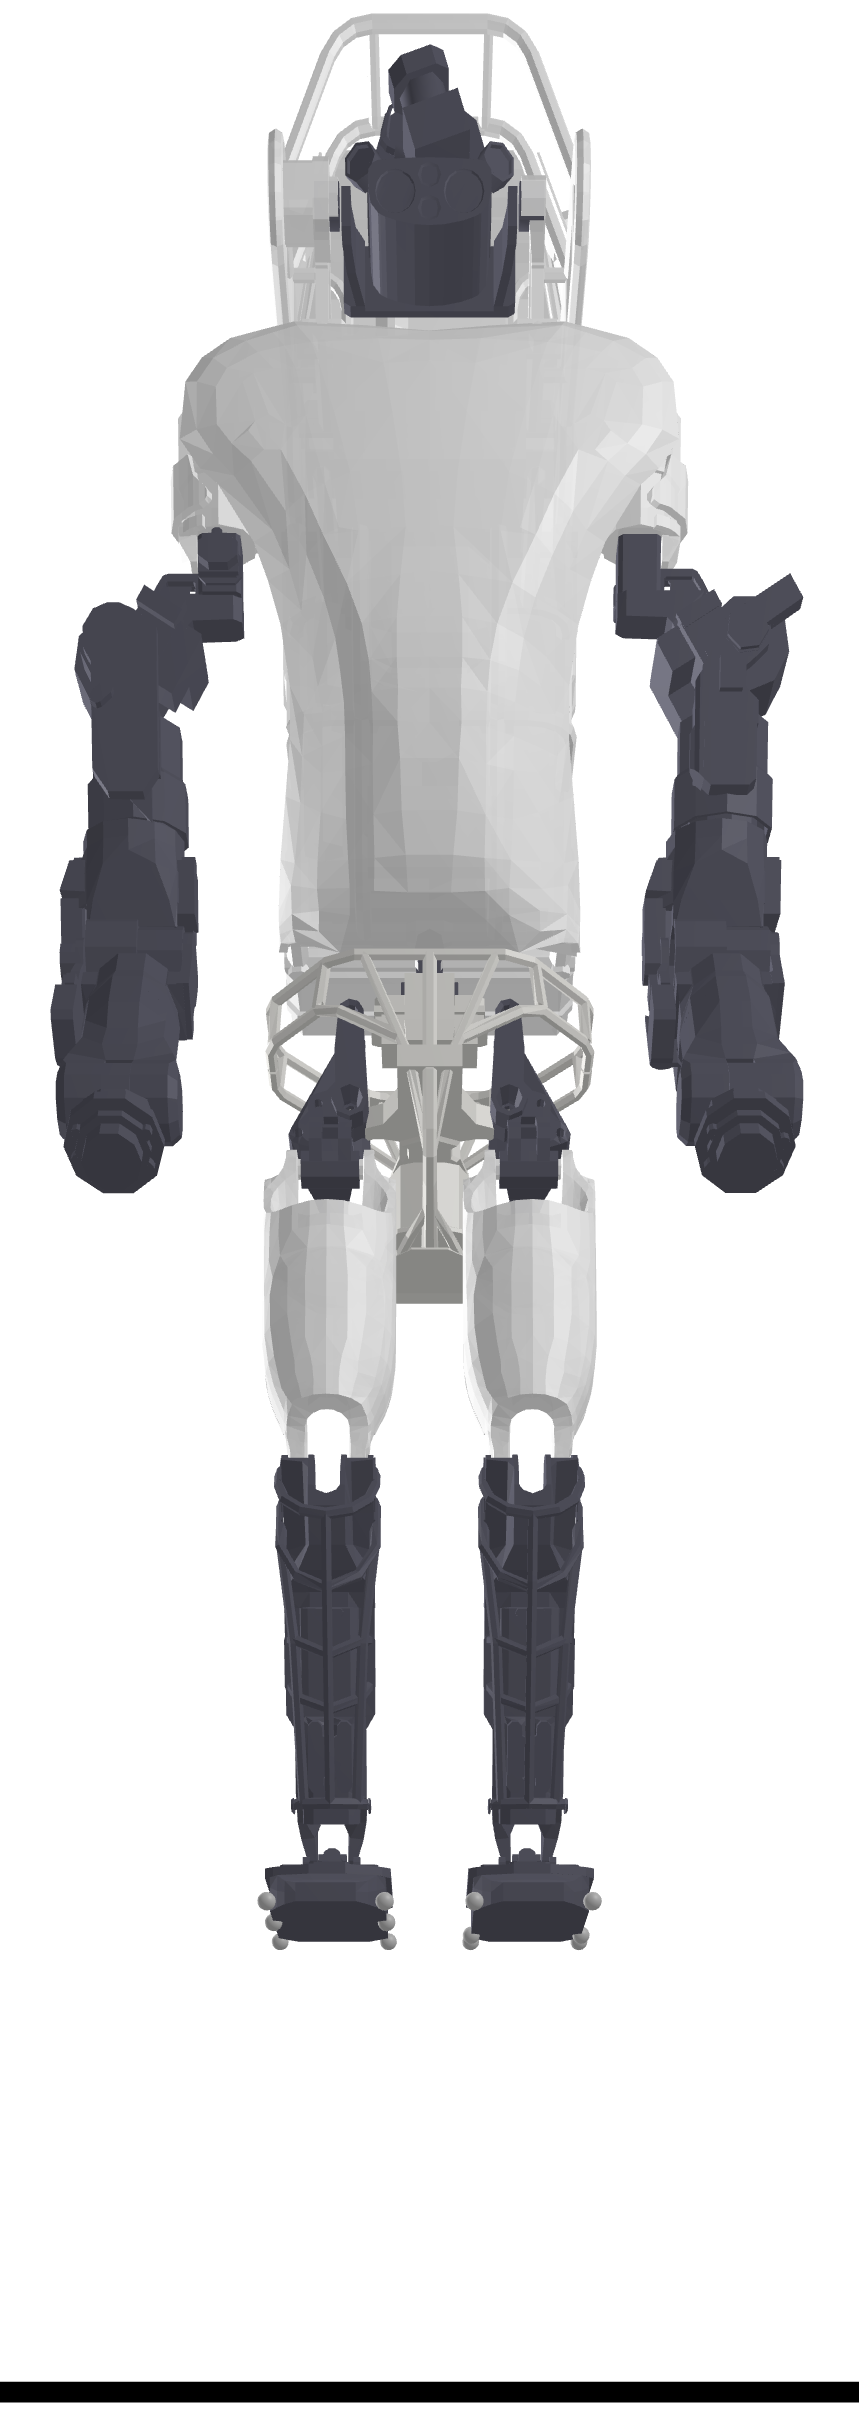
\includegraphics[height=5.0cm]{dojo/atlas1.png} 
	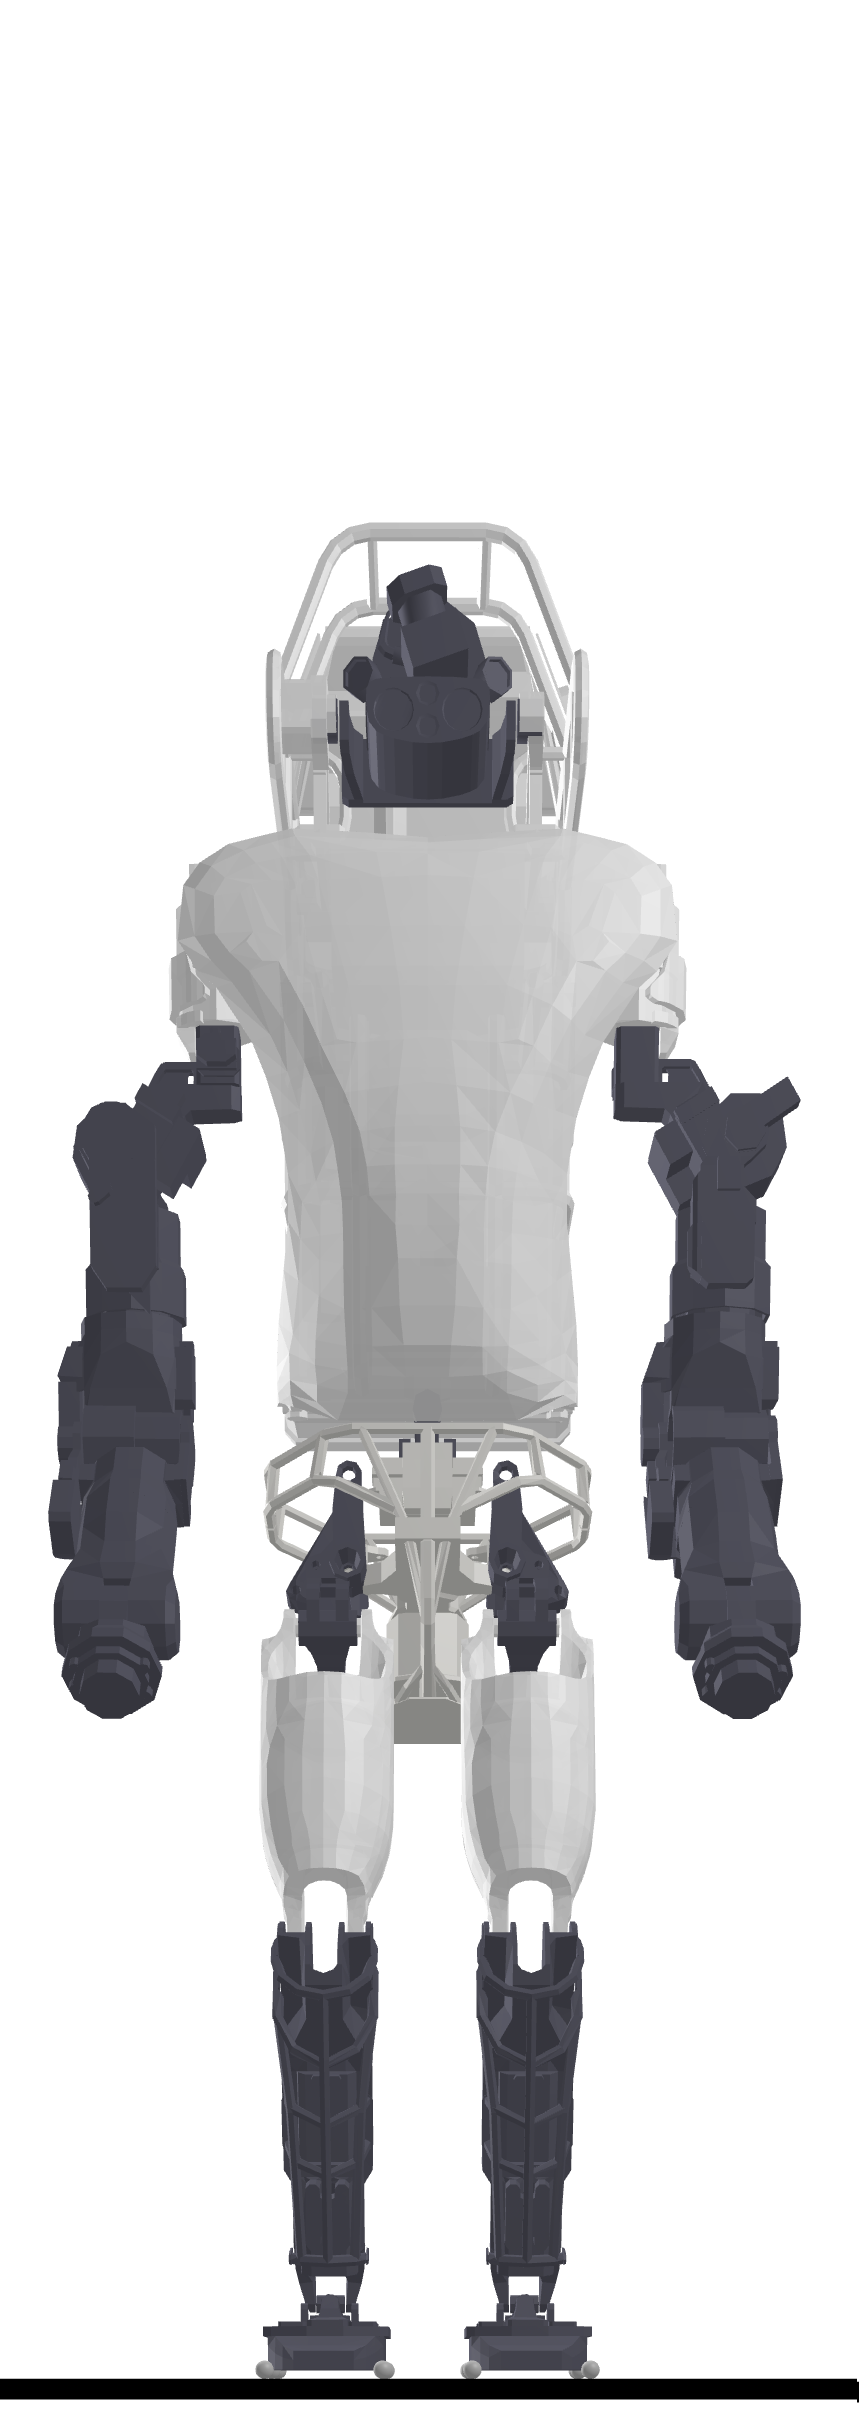
\includegraphics[height=5.0cm]{dojo/atlas2.png}
	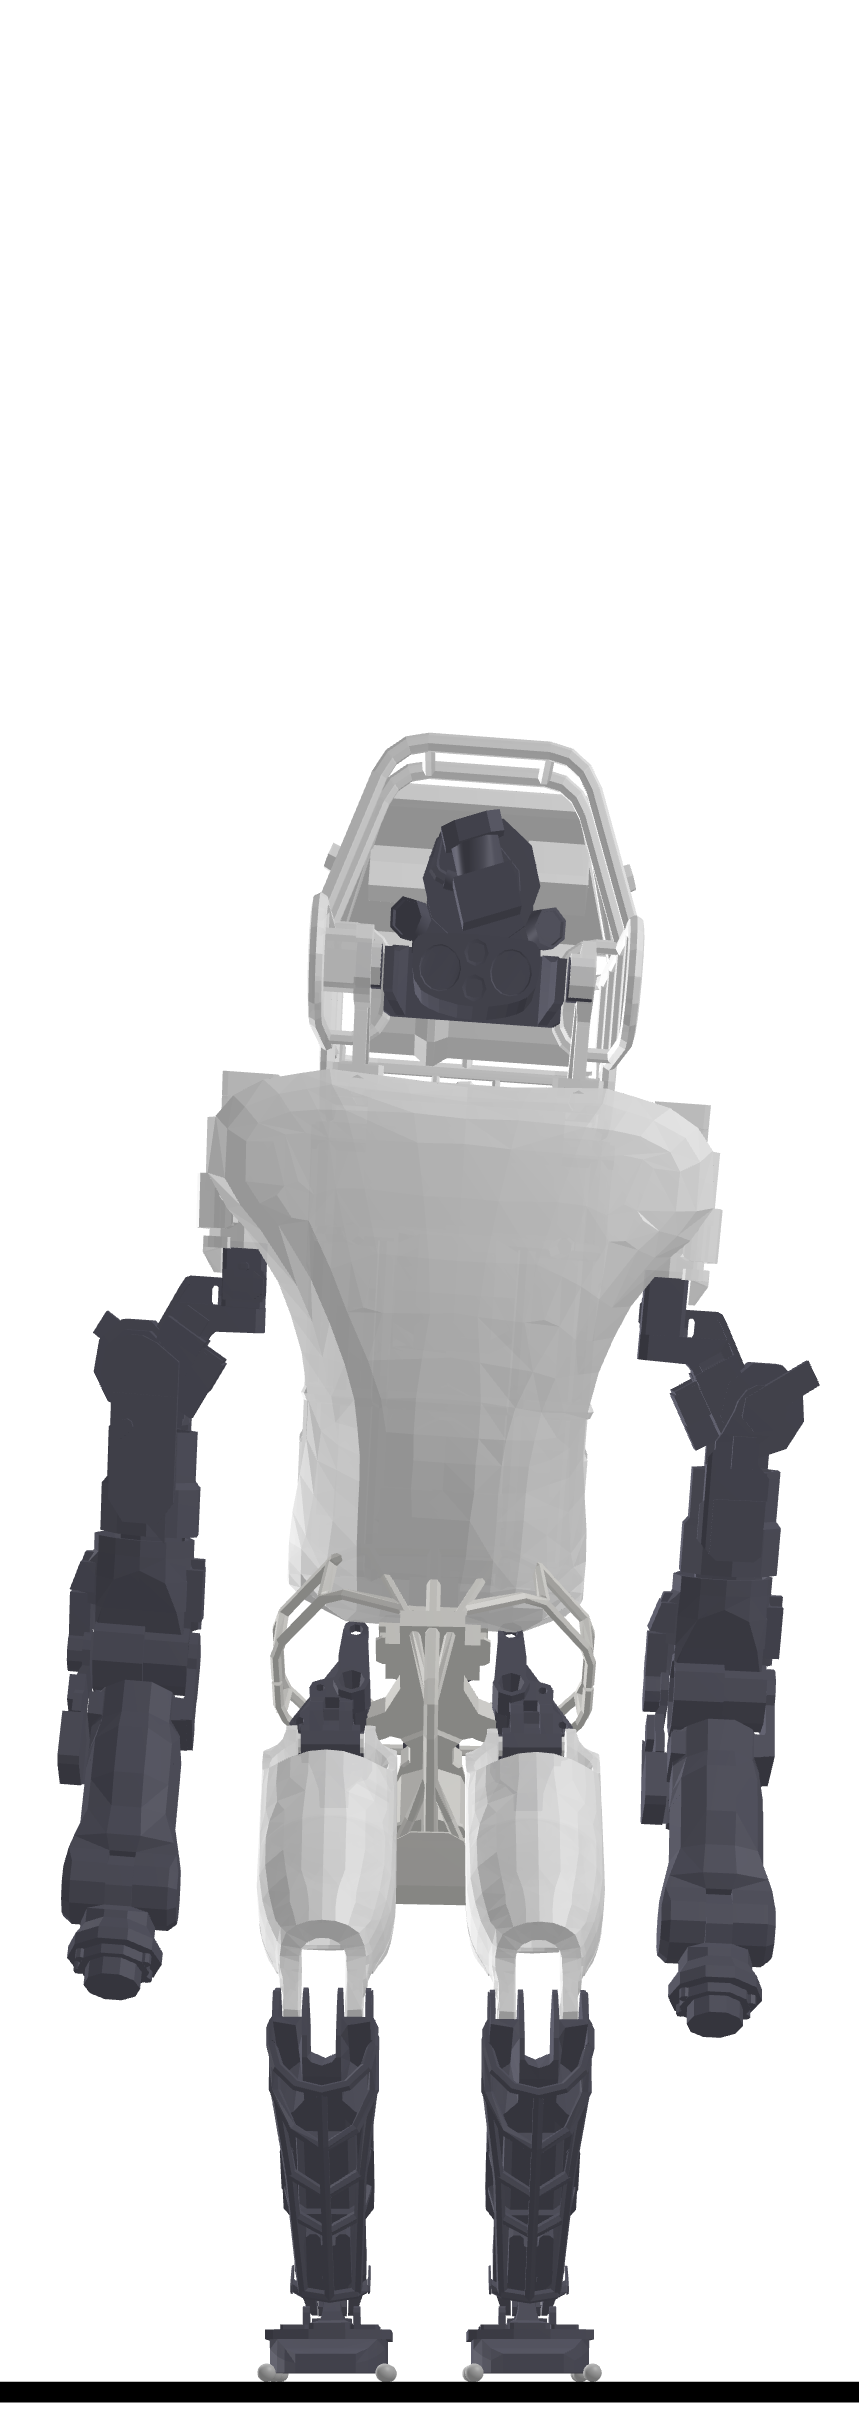
\includegraphics[height=5.0cm]{dojo/atlas3.png}
	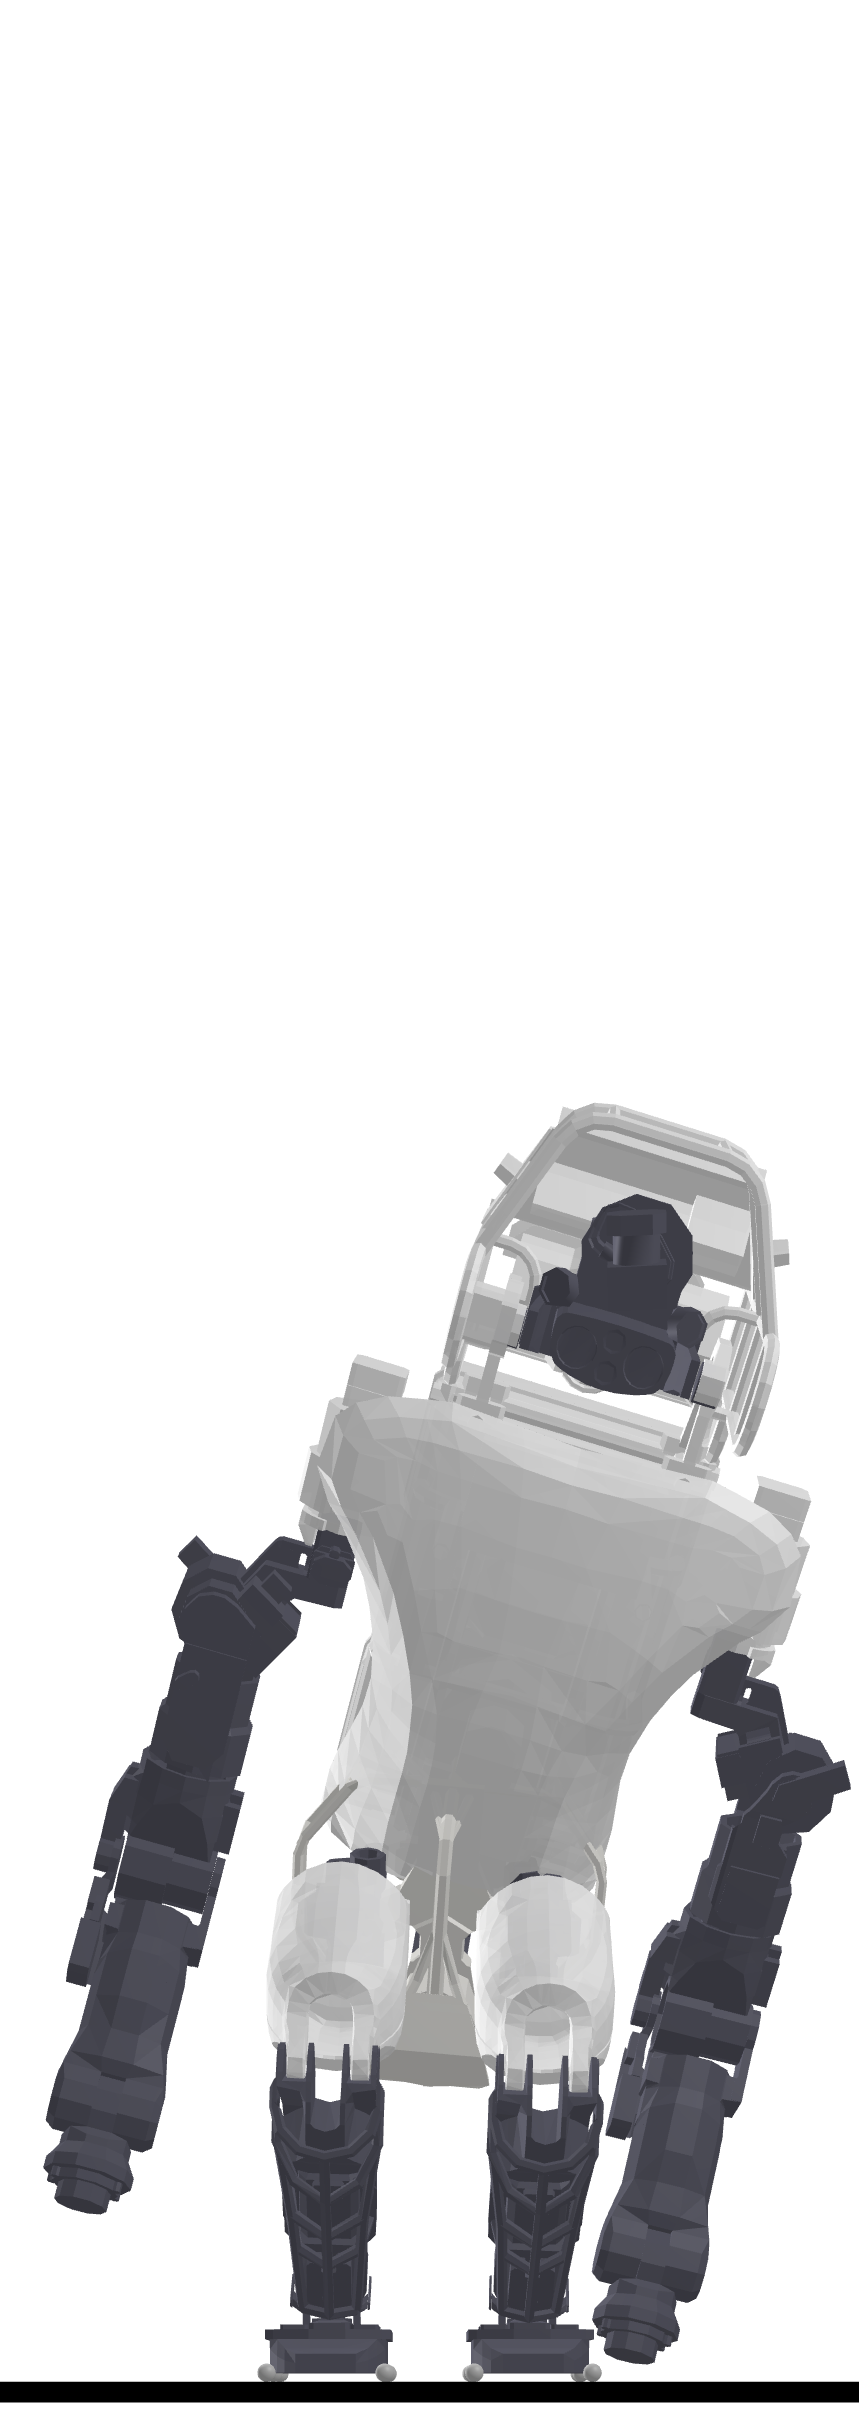
\includegraphics[height=5.0cm]{dojo/atlas4.png}
	\caption[Atlas drop test simulation]{Atlas drop simulation. Dojo simulates this system with 403 maximal-coordinates states, 30 joint constraints, 36 inputs, and 8 contact points in real-time at 65 Hz. Dojo respects floor-feet penetration constraints to machine precision, while MuJoCo suffers from centimeters of interpenetration and is unstable at low simulation rates.}
	\label{dojo_atlas_drop}
\end{figure}

A comparison with MuJoCo is performed measuring penetration violations with the floor for different simulation rates (Table \ref{dojo_contact_violation_results}).

\begin{table}[H]
	\centering
	\caption[Contact violation comparison between Dojo and MuJoCo for Atlas drop test]{Contact violation for Atlas drop. Comparison between Dojo and MuJoCo for foot contact penetration  (millimeters) with the floor for different time steps (seconds). Dojo strictly enforces no penetration. When Atlas lands, its feet remains above the ground by an infinitesimal amount. In contrast, MuJoCo exhibits significant penetration through the floor (i.e., negative values).}
	\begin{tabular}{c c c c}
		\toprule
		\textbf{Time Step} & \textbf{0.1} & \textbf{0.01} & \textbf{0.001} \\
		\toprule
		MuJoCo & \mbox{failure} & \textminus 28 & \textminus 46 \\
		Dojo & \textbf{+1e{-}12} & \textbf{+1e{-}7} & \textbf{+8e{-}6} \\
		\toprule
	\end{tabular}
	\label{dojo_contact_violation_results}
\end{table}

\paragraph{Friction-cone comparison.}
The effect of friction-cone approximation is demonstrated by simulating a box that is initialized with lateral velocity before impacting and sliding along a flat surface. For a pyramidal approximation, in the probable scenario where its vertices are not aligned with the direction of motion, velocity drift occurs for a linearized cone implemented in Dojo and MuJoCo (Fig. \ref{dojo_velocity_drift}). 

\begin{figure}[H]
	\begin{center}
		\begin{tikzpicture}
			\draw (0, 0) node[inner sep=0] {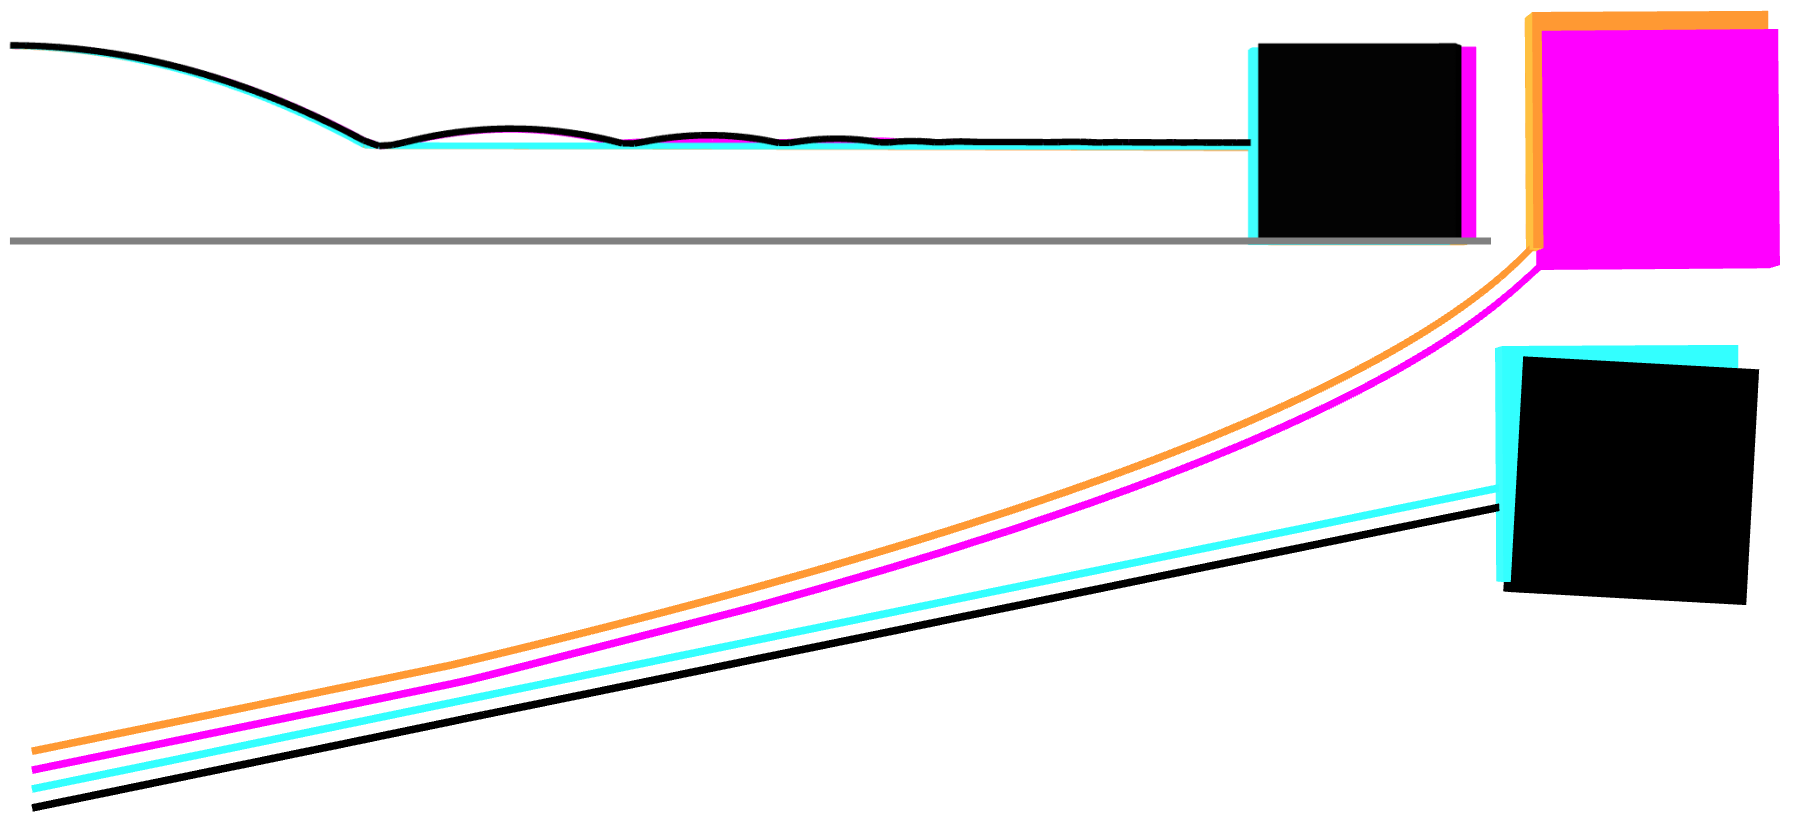
\includegraphics[width=0.5\linewidth]{dojo/cone_compare_final.png}};
			\draw (+0.0, +1.7) node {side view};
			\draw (+0.0, -1.4) node {top view};
		\end{tikzpicture}
	\end{center}
	\caption[Velocity drift comparison between linearized and second-order friction cones]{Velocity drift resulting from friction-cone approximation. Comparison between a box sliding with approximate cones having four vertices implemented in MuJoCo (magenta) and Dojo (orange) versus MuJoCo's (black) and Dojo's (blue) nonlinear friction cones. Dojo's nonlinear friction cone gives the physically correct straight line motion, while linear friction-cone approximations lead to lateral drift. MuJoCo's nonlinear friction cone exhibits a minor rotational drift.}
	\label{dojo_velocity_drift}
\end{figure}

The complementarity problem with $P$ contact points requires $2 P (1 + 2 d)$ decision variables for contact and a corresponding number of constraints, where $d$ is the degree of parameterization (e.g., double parameterization: $d=2$). While it is possible to reduce such artifacts by increasing the number of vertices in the approximation of the second-order cone, this increases the computational complexity. Such approximation is unnecessary in Dojo as we handle the exact nonlinear cone constraint efficiently and reliably with optimization tools from cone programming; the result is accurate sliding.

\paragraph{Energy and momentum conservation.}

An accurate physics engine conserves important physical quantities like energy and momentum. Following the methodology from \cite{erez2015simulation}, we simulate ``astronaut,'' a free-floating humanoid, and measure the drift of these quantities (Fig. \ref{dojo_drift}). 

\begin{figure}[H]
	\centering
	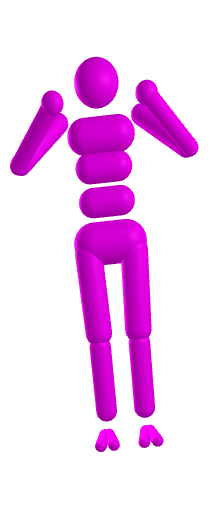
\includegraphics[height=3.8cm]{dojo/astronaut1.png} 
	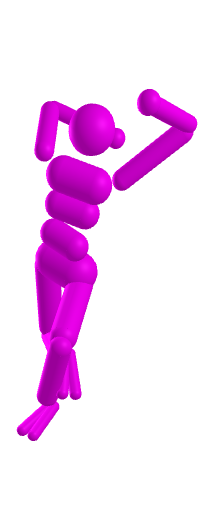
\includegraphics[height=3.8cm]{dojo/astronaut2.png}
	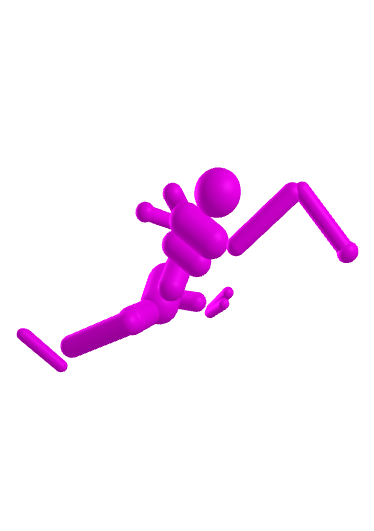
\includegraphics[height=3.8cm]{dojo/astronaut3.png}
	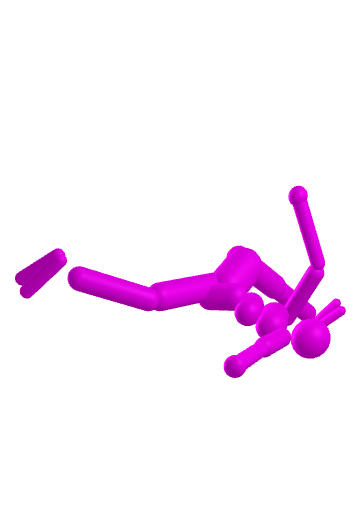
\includegraphics[height=3.8cm]{dojo/astronaut4.png}
	\caption[Astronaut energy and momentum drift simulation]{Astronaut simulation for energy and momentum conservation test. Joints are initialized with zero velocities and randomly actuated for 1 second. The simulation is visualized, from left to right.}
	\label{dojo_astronaut}
\end{figure}

There is no internal damping or springs, joint limits, or contact, and gravity is turned off. The astronaut is initialized with no linear or angular velocity and momentum drift is computed after one second of uniformly sampled actuation: $u \sim \mathcal{U}(0,0.05)$. Energy drift is computed over a 100 second period after 1 second of random actuation. MuJoCo exhibits drift in all scenarios. Characteristic of its variational integrator, Dojo conserves both linear and angular momentum to machine precision. Energy does not drift for Dojo but exhibits small bounded oscillations that decrease in amplitude as the time step decreases (Fig. \ref{dojo_drift}). Conservation of energy to machine precision with variational integrators is possible and is a topic of current research \cite{sharma2018energy}.

\begin{figure}[H]
	\begin{center}
		\includegraphics[width=0.4\columnwidth, height=6.0cm]{dojo/astronaut_energy.tikz}
		\includegraphics[width=0.5\columnwidth, height=6.0cm]{dojo/astronaut_momentum_freq.tikz}
	\end{center}
	\caption[Astronaut energy and momentum drift numerical comparison between Dojo and MuJoCo]{
		Energy and momentum conservation comparison between MuJoCo and Dojo for the astronaut simulation (Fig \ref{dojo_astronaut}) using time steps ranging from 0.001 to 0.1 second. Momentum drift is measured after actuating the astronaut for 1 second with random controls. Energy drift is measured over a 100 second simulation after 1 second of random actuation.}
	\label{dojo_drift}
\end{figure}

\subsection{Planning} 

Iterative LQR \cite{howell2022trajectory} utilizes implicit gradients from Dojo to perform trajectory optimization on three systems: planar box, hopper, and quadruped. A comparison is performed with MuJoCo and finite-difference gradients. The results for the quadruped are visualized in Fig. \ref{dojo_trajopt_vis} and all tested systems are summarized in Table \ref{dojo_trajopt_results}. 

\begin{figure}[H]
	\centering
	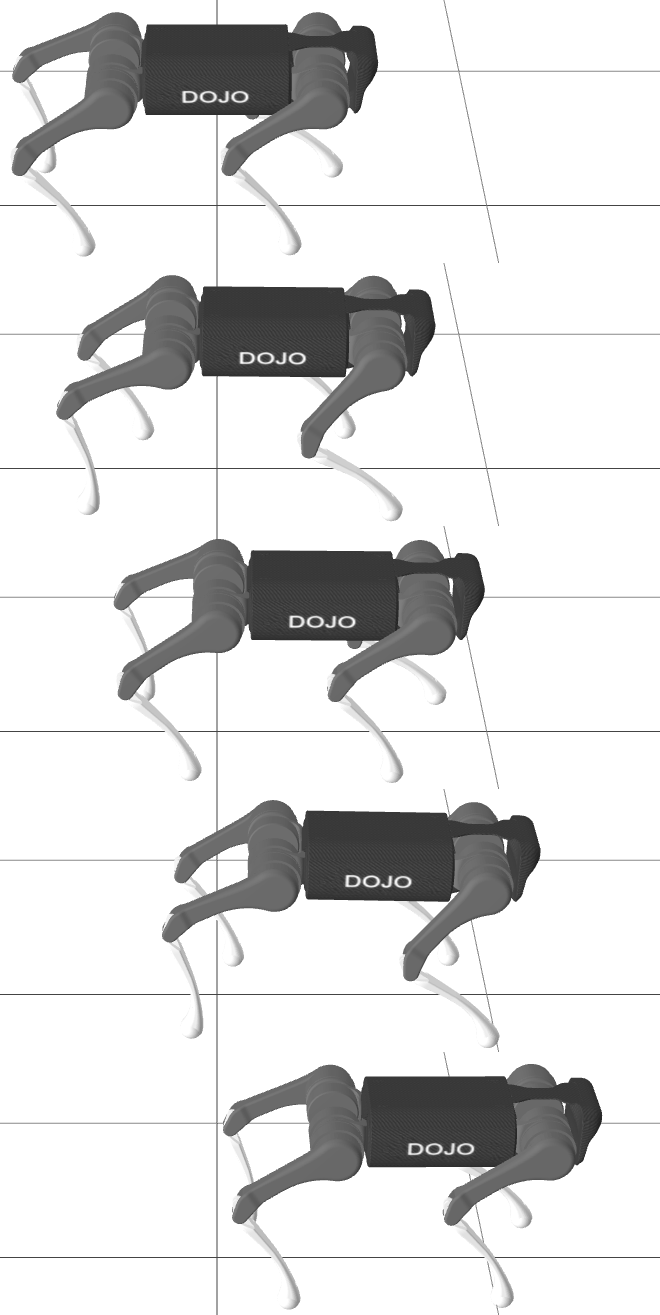
\includegraphics[width=0.25\textwidth]{dojo/quadruped_stack.png}
	\caption[Locomotion plan for quadruped]{Locomotion plan for quadruped generated using trajectory optimization. Time progresses top to bottom.}
	\label{dojo_trajopt_vis}
\end{figure}

\paragraph{Box.} Inputs are optimized to move a stationary rigid body that is resting on a flat surface (Fig. \ref{dojo_gradient_compare}) to a goal location that is either to the right or up in the air $1$ meter. The planning horizon is $1$ second and the controls are initialized with zeros. Dojo uses a time step $h = 0.1$, whereas MuJoCo uses $h = 0.01$ to prevent significant contact violations with the floor. MuJoCo fails in the scenario with the goal in the air, while Dojo succeeds at both tasks.

\paragraph{Hopper.} The hopping robot \cite{raibert1989dynamically} with $m = 3$ controls and $n = 14$ degrees-of-freedom is tasked with moving to a target pose over $1$ second. Similar, although not identical, models and costs are used. Dojo uses a time step $h = 0.05$ whereas MuJoCo uses $h = 0.01$. The hopper is initialized with controls that maintain its standing configuration. Quadratic costs are used to penalize control effort and cost shaping is utilized to set target positions in the air and the goal pose. The optimizer typically finds a single-hop motion.

\paragraph{Quadruped.} The torque-controlled Unitree A1 quadruped \cite{unitree2022a1} with $m = 12$ controls and $n = 36$ degrees-of-freedom is tasked with moving to a goal location over a planning horizon $T = 41$ with time step $h = 0.05$. Controls are initialized to compensate for gravity and there are costs on tracking a target kinematic gait and control inputs. The optimizer finds a dynamically feasible motion that closely tracks the kinematic plan.

\begin{table}[H]
	\centering
	\caption[Numerical planning results for box, hopper, and quadruped]{Planning results. Comparison of final cost value, goal constraint violation, and total number of iterations for a collection of systems with maximal (max) and minimal (min) representations, optimized with iterative LQR \cite{li2004iterative} using Dojo with implicit gradients or MuJoCo (M) with finite-difference gradients.}
	\begin{tabular}{c c c c}
		\toprule
		\textbf{System} & \textbf{Cost} & \textbf{Violation} & \textbf{Iterations}\\
		\toprule
		box right (max) & 14.5 & 3e{-}3 & \textbf{30} \\
		box right (M) & \textbf{13.5} & \textbf{3e{-}3} & 95 \\
		\hline
		box up (max) & \textbf{14.5} & \textbf{3e{-}3} & \textbf{106} \\
		box up (M) & \mbox{failure} & 1.0 & -\\
		\hline
		hopper (max) & 10.2 & 4e{-}3 & \textbf{57} \\
		hopper (min) & \textbf{8.9} & \textbf{1e{-}3} & 96 \\
		hopper (M) & 26.7 & 2e{-}3 & 66 \\
		\hline
		quadruped (min) & 2e{-}2 & 3e{-}4 & 20 \\
		\toprule
	\end{tabular}
	\label{dojo_trajopt_results}
\end{table}

In the examples, gradients are computed with $\kappa = 3e{-}4$. Overall, we find that final results from both engines are similar. However, importantly, MuJoCo is enforcing soft contact whereas Dojo simulates hard contact. Further, MuJoCo requires a time step $h = 0.01$ for stable simulation, whereas Dojo works well with $h = 0.05$. 

\subsection{Policy optimization}

Gym-like environments \cite{brockman2016openai, duan2016benchmarking}: ant and half-cheetah are implemented in Dojo and we train static linear policies for locomotion. As a baseline, we employ Augmented Random Search (ARS) \cite{mania2018simple}, a gradient-free approach coupling random search with a number of simple heuristics. For comparison, we train the same policies using augmented gradient search (AGS) which replaces the stochastic-gradient estimation of ARS with the Dojo's implicit gradients. Policy rollouts are visualized in Fig. \ref{dojo_rl_vis} and results are summarized in Table \ref{dojo_rl_results}.

\begin{figure}[H]
	\begin{center}
		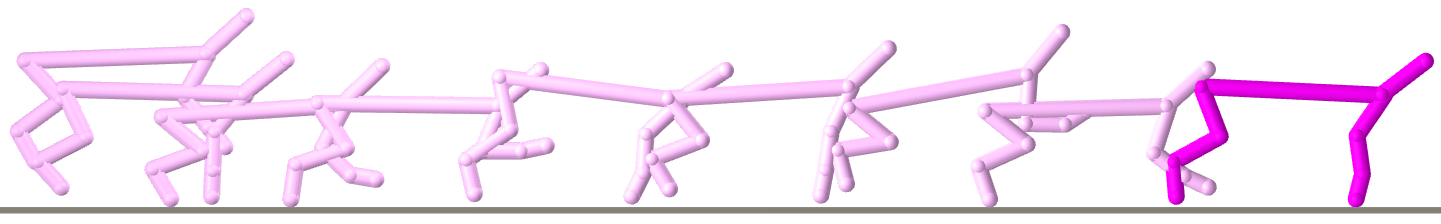
\includegraphics[width=0.5\columnwidth]{dojo/halfcheetah_ars.png}
		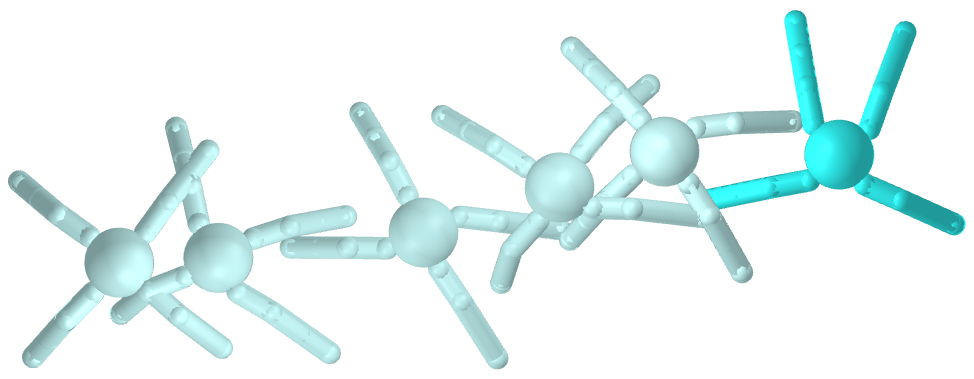
\includegraphics[width=0.5\columnwidth]{dojo/ant_ars.png}
	\end{center}
	\caption[Learned policy rollouts for half-cheetah and ant]{Learned policy rollouts for half-cheetah (top) and ant (bottom) generated using Augmented Random Search. Time progresses left to right.}
	\label{dojo_rl_vis}
\end{figure}

\paragraph{Half-cheetah.}
This planar system \cite{brockman2016openai} with $m = 6$ controls and $n = 18$ degrees-of-freedom is rewarded for forward velocity and penalized for control effort over a horizon $T = 80$ with time step $h = 0.05$. 

\paragraph{Ant.}
The system \cite{brockman2016openai} has $m = 8$ controls and $n = 28$ degrees-of-freedom and is rewarded for forward motion and staying alive and is penalized for control effort and contact over a horizon $T = 150$ with time step $h = 0.05$.

\begin{table}[H]
	\centering
	\caption[Numerical policy optimization results for half-cheetah and ant]{Policy optimization results. Comparison of total reward, number of simulation-step and gradient evaluations for policies trained with Augmented Random Search (ARS) \cite{mania2018simple} and Augmented Gradient Search (AGS). The results are averaged over the best 3 out of 5 runs with different random seeds.} 
	\begin{tabular}{c c c c}
		\toprule
		\textbf{System} & \textbf{Reward} & \textbf{Simulation} & \textbf{Gradient} \\
		\toprule
		half-cheetah (ARS) & 46 $\pm$ 24 & 3e{+}4 & 0 \\
		ant (ARS)          & 64 $\pm$ 15 & 2e{+}5 & 0 \\
		half-cheetah (AGS) & 44 $\pm$ 24 & \textbf{5e{+}3} & 5e{+}3 \\ 
		ant (AGS)          & 54 $\pm$ 28 & \textbf{2e{+}4} & 2e{+}4 \\
		\toprule
	\end{tabular}
	\label{dojo_rl_results}
\end{table}

First, we are able to successfully train policies using this simple learning algorithm in Dojo's hard contact environments. Second, MuJoCo requires smaller $h = 0.01$ time steps for stable simulation, whereas Dojo is stable with $h = 0.05$. Third, our initial experiments indicate that it is possible to utilize Dojo's implicit gradients for more efficient training compared to the derivative-free approach.

\subsection{System identification} 

System identification is performed on an existing real-world dataset of trajectories collected by throwing a box on a table with different initial conditions \cite{pfrommer2021contactnets}. We learn a set of parameters $\theta = (\mu, p^{(1)}, \dots, p^{(8)})$ that include the friction coefficient $\mu$, and 3-dimensional vectors $p^{(i)}$ that represent the position of vertex $i$ of the box with respect to its center of mass.

Each trajectory is decomposed into $T-2$ triplets of consecutive configurations: $Z = (z_{-}, z, z_{+})$, where $T$ is the number of time steps in the trajectory. Using the initial conditions $z_{-}, z$ from a tuple, and an estimate of the system's parameters $\theta$, Dojo performs one-step simulation to predict the next state, $\hat{z}_{+}$. Implicit gradients are utilized by a Gauss-Newton method to learn the system parameters.

\begin{figure}[t]
	\begin{center}
		\begin{tikzpicture}
			\draw (0, 0) node[inner sep=0] {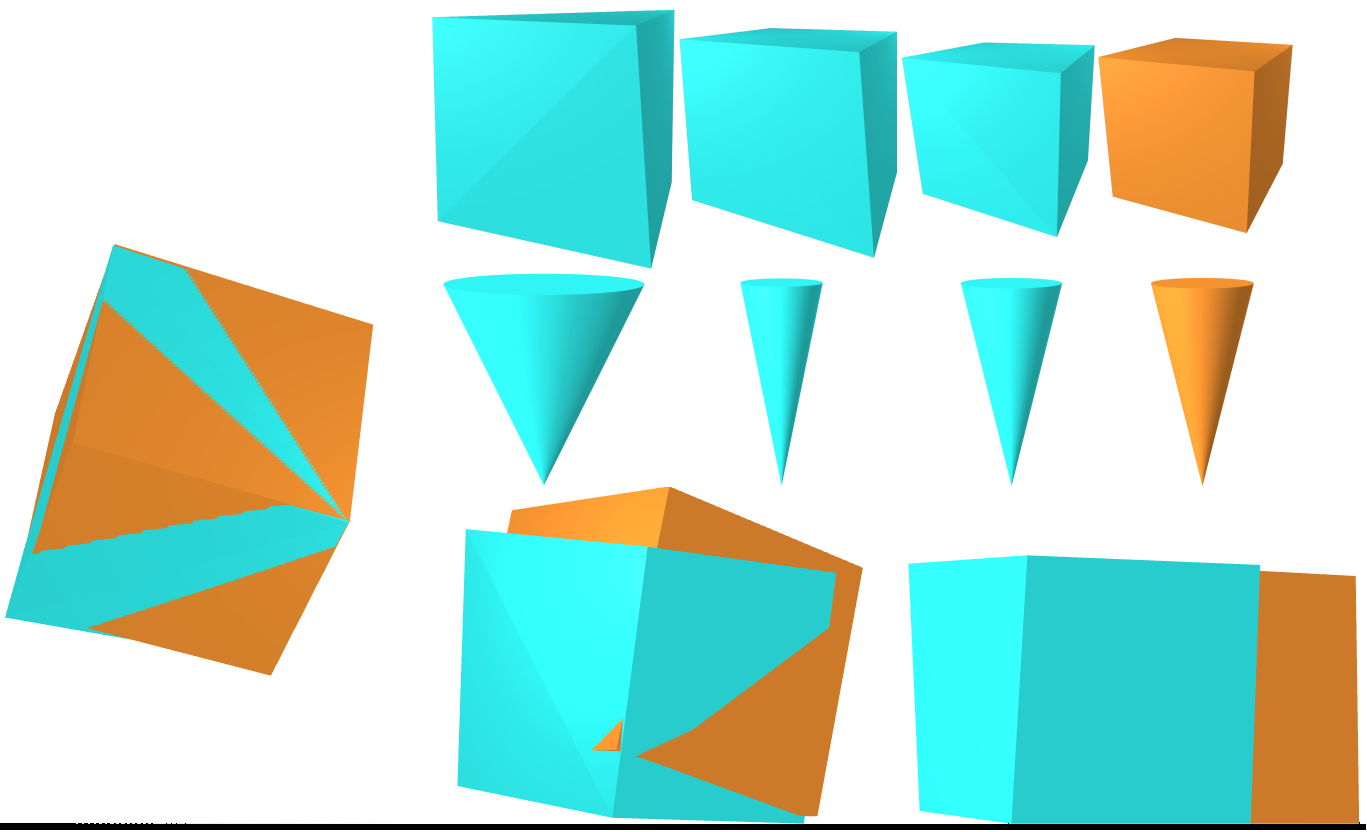
\includegraphics[width=0.5\linewidth]{dojo/box_and_cone_and_toss.png}};
			\draw (-0.7, +2.9) node {(1)};
			\draw (+0.6, +2.9) node {(5)};
			\draw (+1.8, +2.9) node {(50)};
			\draw (+2.95, +2.9) node {(truth)};
		\end{tikzpicture}
	\end{center}
	
	\caption[Learned friction parameters and contact geometry for box (top). Real-to-sim simulation for learned box parameters (bottom)]{System identification. Top right: Learning box geometry and friction cone to less than $5\%$ error. Bottom: Simulated trajectory of the box using the learned properties (blue) compared to ground truth (orange).}
	\label{dojo_real2sim}
\end{figure}

The parameters are learned by minimizing the following loss: 
\begin{align}
	\mathcal{L}(\mathcal{D}, \theta) = \sum_{Z \in \mathcal{D}} L(Z, \theta) = \sum_{Z \in \mathcal{D}} \frac{1}{2} ||\mbox{\textbf{Dojo}}(z_{-}, z; \theta) - z_{+}||_W^2,
\end{align}
where $||\cdot||_W$ is a weighted norm, which aims to minimize the difference between the ground-truth trajectories and physics-engine predictions. We use gradients:
\begin{equation}
	\frac{\partial L}{\partial \theta} = {\frac{\partial \mbox{\textbf{Dojo}}}{\partial \theta}}^T W \left(\mbox{\textbf{Dojo}}(z_{-}, z; \theta) - z_{+} \right),
\end{equation}
and approximate Hessians: 
\begin{align}
	\frac{\partial^2 L}{\partial \theta^2} &\approx {\frac{\partial \mbox{\textbf{Dojo}}}{\partial \theta}}^T W \frac{\partial \mbox{\textbf{Dojo}}}{\partial \theta}.
\end{align}
Gradients are computed with $\kappa = 3e{-}4$.

After training, the learn parameters are within $5\%$ of the geometry and best-fit friction coefficient for the box from the dataset. We complete the transfer from real-to-sim and simulate the learned system parameters in Dojo, comparing it to the ground-truth dataset trajectories. Results are visualized in Fig. \ref{dojo_real2sim}.

\section{Limitations} \label{dojo_limitations}

The computation cost of Dojo per simulation step is greater than many existing engines. The greater computational complexity enables superior simulation accuracy at the cost of increased wall-clock time and is a trade-off that must be considered by the user for a particular application. Additionally, because Dojo solves a nonlinear complementarity problem (i.e, non-convex problem) at each time step the engine provides no guarantees of converging to a solution. In practice, we do no find this to be a problem, but for time- or safety-critical applications this should be a consideration. Further, it remains to be seen how well sim-to-real transfer works, in comparison to existing engines, particularly for manipulation tasks with a large number of contact interactions.

\section{Future work} \label{dojo_future_work}

Dojo is designed from physics- and optimization-first principles to enable better gradient-based optimization for motion planning, control, reinforcement learning, and system identification. The engine makes several advancements over previous state-of-the-art engines for robotics: First, the variational integrator enables stable simulation at low sample rates. Second, the contact model includes an improved friction model that eliminates artifacts like creep, particularly for sliding, and hard contact for impact is achieved to machine precision. This should enable superior sim-to-real transfer for both locomotion and manipulation applications. The underlying interior-point solver, developed specifically for solving NCPs, is numerically robust and requires practically no hyperparameter tuning for good performance across numerous systems, and handles cone and quaternion variables. Third, the engine efficiently returns implicit gradients that are smooth and analytical, providing useful information through contact events. Fourth, in addition to building and providing an open-source tool, the physics and optimization algorithms presented can improve many existing engines.

In terms of features, reliability, and wall-clock time, MuJoCo--the product of a decade of excellent software engineering--is impressive. As development of Dojo continues, we expect to make significant progress in all of these areas. However, fundamentally, Dojo's approach of solving an NCP with a primal-dual interior-point method will likely be computationally more expensive compared to MuJoCo's convex soft-contact model, which can never entirely recover accurate solutions even at higher sampling frequencies. This is the fundamental trade-off Dojo makes for robotics applications: greater computational cost for accurate physics and smooth gradients.

A number of future improvements to Dojo are planned. First, Dojo currently implements simple collision detection (e.g., sphere-halfspace, sphere-sphere). Natural extensions include support for convex primitives and curved surfaces. Another improvement is adaptive time stepping. Similar to advanced numerical integrators for stiff systems, Dojo should take large time steps when possible and adaptively modify the time step in cases of numerical difficulties or physical inaccuracies. Finally, hardware-accelerator support for Dojo would potentially enable faster simulation and optimization.

Perhaps the most important remaining question is whether the physics and optimization improvements from this work translate into better transfer of simulation results to successes on real-world robotic hardware. In this thrust, future work will explore the transfer of control policies trained in Dojo to hardware and deployment of the engine in model predictive control frameworks.

In conclusion, we have presented a new physics engine, Dojo, specifically designed for robotics. This tool is the culmination of a number of improvements to the contact dynamics model and underlying optimization routines, aiming to advance state-of-the-art physics engines for robotics by improving physical accuracy and differentiability. 

\section*{Acknowledgments}
The authors would like to thank Jan Br{\"u}digam for  \texttt{ConstrainedDynamics.jl}, an open-source library which served as a foundation for Dojo's maximal-coordinates state representation, as well as early technical discussions and support; and Suvansh Sanjeev for assistance with the Python interface. Toyota Research Institute provided funds to support this work. 

\section{Appendix: Quaternion Algebra}
\label{dojo_quaternion_algebra}
In this section we introduce a set of conventions for notating standard quaternion operations, adopted from \cite{brudigam2020linear,jackson2021planning}, and employed in the rotational part of our variational integrator \eqref{dojo_rotational_integrator}.

Quaternions are written as four-dimensional vectors:
\begin{equation}
	q = (s, v) = (s, v_1, v_2, v_3) \in \mathbf{H},
\end{equation}
where $s$ and $v$ are scalar and vector components, respectively. Dojo employs unit quaternions (i.e., $q^T q = 1$) to represent orientation, providing a mapping from the local body frame to a global inertial frame.

Quaternion multiplication is represented using linear algebra (i.e., matrix-vector and matrix-matrix products). Left and right quaternion multiplication, 
\begin{equation} 
	q^a \otimes q^b 
	= \begin{bmatrix}
		s^a s^b - (v^a)^T v^b \\
		s^a v^b + s^b v^a + v^a \times v^b
	\end{bmatrix} 
	= L(q^a)q^b = R(q^b) q^a ,
\end{equation}
where $\times$ is the standard vector cross product, is represented using the matrices:
\begin{align}
	L(q) &= \begin{bmatrix}
		s & -v^T \\
		v & s I_3 + \mathbf{skew}(v)
	\end{bmatrix} \in \mathbf{R}^{4 \times 4},\\
	R(q) &= \begin{bmatrix}
		s & -v^T \\
		v & s I_3 - \mathbf{skew}(v)
	\end{bmatrix} \in \mathbf{R}^{4 \times 4},
\end{align}

where, 
\begin{equation}
	\mathbf{skew}(x) = \begin{bmatrix}  
		0 & -x_3 & x_2 \\
		x_3 & 0 & -x_1 \\
		-x_2 & x_1 & 0 
	\end{bmatrix},
\end{equation}
is defined such that,
\begin{equation}
	\mathbf{skew}(x) y = x \times y ,
\end{equation}
and $I_3$ is a 3-dimensional identity matrix. The vector component of a quaternion, 
\begin{equation} 
	v = V q,
\end{equation}
is extracted using the matrix:
\begin{equation}
	V = \begin{bmatrix}
		\mathbf{0} & I_3
	\end{bmatrix} \in \mathbf{R}^{3 \times 4},
\end{equation}
and quaternion conjugate: 
\begin{equation} 
	q^{\dagger} = \begin{bmatrix} s \\ -v \end{bmatrix} = T q,
\end{equation}
is computed using:
\begin{equation}
	T = \begin{bmatrix}
		1 & \mathbf{0}^T \\
		\mathbf{0} & -I_3
	\end{bmatrix} \in \mathbf{R}^{4 \times 4}.
\end{equation}
	


\chapter{Fast Constrained Trajectory Optimization}

Trajectory optimization is a widely used tool with many important applications in robotic motion planning and control. However, most existing algorithm implementations fall into one of two categories: either they rely on general-purpose off-the-shelf solvers for non-convex problems that are numerically robust and capable of handling constraints but tend to be slow, or they use custom numerical methods that are fast but lack robustness and have limited or no ability to deal with constraints. This chapter presents ALTRO (Augmented Lagrangian TRajectory Optimizer), a novel algorithm for solving constrained trajectory optimization problems that bridges this gap by offering fast convergence, numerical robustness, and the ability to handle general state and action constraints.

\vspace*{\fill}

\noindent ALTRO: A Fast Solver for Constrained Trajectory Optimization. Taylor A. Howell$^*$, Brian Jackson$^*$, and Zachary Manchester. International Conference on Intelligent Robots and Systems. 2019.

\pagebreak

\section{Introduction}
Trajectory optimization is a powerful tool for planning, enabling the synthesis of dynamic motions for complex underactuated robotic systems. This general framework can be applied to robots with nonlinear dynamics and constraints where other motion planning paradigms---such as sample-based planning, inverse dynamics, or differential flatness---are impractical or ineffective.

Direct methods transcribe states and actions as decision variables and solve (\ref{intro_trajopt}) using general-purpose solvers such as SNOPT \cite{gill2005snopt} or Ipopt \cite{wachter2006implementation}, and tend to be versatile and robust. It is straight forward to provide an initial state trajectory to the solver in such methods, even if it is dynamically infeasible. Direct transcription \cite{pardo2016evaluating} and direct collocation \cite{hargraves1987direct} are common direct algorithms. 

Alternatively, indirect methods leverage the structure of (\ref{intro_trajopt}) to solve a sequence of smaller sub-problems using dynamic programming. These are anytime algorithms, meaning they are always dynamically feasible, allowing state and action trajectories at any iteration to be used in a tracking controller. However, it is often difficult to find a suitable initial guess for the action trajectory. Historically, indirect methods have been considered less robust and less suitable for reasoning about general state and action constraints, but they tend to be fast and amenable to implementation in embedded systems. Methods include Differential Dynamic Programming (DDP) \cite{mayne1966second} and Iterative LQR (iLQR)\cite{li2004iterative}, as well as various shooting methods~\cite{keller2018numerical}. 

In this chapter we present ALTRO (Augmented Lagrangian TRajectory Optimizer), a trajectory optimization algorithm that combines the best characteristics of both direct and indirect methods, namely: speed, small problem size, numerical robustness, handling of state and action constraints, anytime dynamic feasibility, and infeasible state initialization. Our contributions are a number of enhancements to an algorithm that utilizes iLQR within an augmented Lagrangian framework to handle constraints, including:
\begin{itemize}
	\item a numerically robust square-root backward pass
	\item reformulations for infeasible initialization and free-time problems
	\item a solution polishing phase that returns highly accurate solutions
\end{itemize} 

In the remainder of the chapter, Section \ref{altro_related_work} provides an overview of related work. Then, Section \ref{altro_background} provides background on inequality-constrained augmented Lagrangian methods and matrix square roots. Next, we present ALTRO in Section \ref{altro_algorithm}. In Section \ref{altro_results} we highlight these solver enhancements with examples including a cart-pole and car. Finally, we discuss the algorithm's limitations in Section \ref{altro_limitations} and directions for future work in Section \ref{altro_future_work}.

\section{Related Work} \label{altro_related_work}
Several methods have been proposed to incorporate constraints into indirect methods: box constraints on actions \cite{tassa2014control} and stage-wise inequality constraints on the states \cite{xie2017differential,lin1991differential} have been handled by solving a constrained quadratic program at each step of the backward pass; a projection method was devised that satisfies linearized terminal state and stage state-action constraints \cite{giftthaler2018family}; augmented Lagrangian methods have been proposed \cite{plancher2017constrained}, including hybrid approaches that also solve constrained quadratic programs for stage state-action constraints \cite{lantoine2012hybrid,lin1991differential}; and mixed state-action constraints have also been handled using a penalty method \cite{farshidian2017efficient}. 

\section{Background} \label{altro_background}
In this section we provide background on optimizing inequality-constrained problems using augmented Lagrangian methods and matrix square roots.

\paragraph{Inequality-constrained augmented Lagrangian method.}
Classically, augmented Lagrangian methods are utilized to handle equality-constrained optimization problems \eqref{intro_equality_constrained}. However, with small modifications to the algorithm it is possible to also handle inequality constraints \cite{toussaint2014novel}. 

For mixed problems:
\begin{equation}
	\begin{array}{ll}
		\underset{x}{\mbox{minimize }}  & c(x) \\
		\mbox{subject to } & g(x) \, \{\leq,=\}\, 0, \\
	\end{array}
	\label{altro_equality_inequality_constrained}
\end{equation}
we formulate an augmented Lagrangian with indicator penalties:
\begin{equation}
L_{\mathcal{A}}(x; \lambda, \rho) = c(x) + \lambda^T g(x)  +\frac{1}{2}g(x)^T I_{\rho} g(x), \label{altro_augmented_lagrangian_indicator}
\end{equation}
where $I_{\rho}$ is a diagonal matrix defined as:
\begin{equation}
	I_{\rho}^{(i)} = 
	\begin{cases} 
		0 & \text{if } g^{(i)}(x) < 0 \land \lambda^{(i)} = 0 \land \, i \in \mbox{\textbf{inequality}},\\
		\rho & \text{otherwise} .
	\end{cases}
\end{equation}
The dual update becomes:
\begin{equation}\label{altro_dual_update}
	\lambda_{+}^{(i)} = \begin{cases}
		\lambda^{(i)} + \rho g^{(i)}(x) & i \in \mbox{\textbf{equality}}, \\
		\max \Big(0, \lambda^{(i)} + \rho g^{(i)}(x)\Big) & i \in \mbox{\textbf{inequality}},
	\end{cases}
\end{equation} 
and the penalty update:
\begin{equation}\label{altro_penalty_update}
	\rho_{+} = \phi(\rho),
\end{equation}
remains a monotone update. The augmented Lagrangian procedure remains the same: minimize \eqref{altro_augmented_lagrangian_indicator} for fixed duals and penalty values, dual update \eqref{altro_dual_update}, penalty update \eqref{altro_penalty_update}, and repeat until convergence to a desired constraint tolerance is achieved.

\paragraph{Matrix square roots.}
For matrices $A, B \in \mathbf{S}_{++}^{n}$, we can utilize the individual matrix square-roots $\sqrt{A}$ and  $\sqrt{B}$ to compute $\sqrt{A + B}$ as follows:
\begin{align}
	A + B &= [\sqrt{A}^T\, \sqrt{B}^T]\begin{bmatrix} \sqrt{A} \\ \sqrt{B} \end{bmatrix},\\
	&= F^T F, \\
	&= R^T Q^T Q R, \\
	&= R^T R, 
\end{align}
where $F \in \mathbf{R}^{2n \times n}$ is the matrix factorized by a QR decomposition, the product of two orthogonal matrices is the identity (i.e., $Q^T Q = I)$, and the upper triangular matrix returned by the procedure:
\begin{equation}
\sqrt{A + B} = R,
\end{equation} 
is the solution. We define:
\begin{equation}
	\sqrt{A + B} = \mbox{\textbf{QR}}\Big(\begin{bmatrix} \sqrt{A} \\ \sqrt{B} \end{bmatrix}\Big).
\end{equation}
The complexity of this operation is $\mathbf{O}(n^3)$ using the Householder algorithm.

We can also compute $\sqrt{A - B}$ using the individual matrix square-roots. We perform rank-one downdates on $\sqrt{A}$ using the rows of $\sqrt{B}$:
\begin{equation}
	\sqrt{A - B} = \mbox{\textbf{DD}}\Big(\sqrt{A}, \sqrt{B}\Big).
\end{equation}
The complexity of this operation is also $\mathbf{O}(n^3)$.

\section{ALTRO} \label{altro_algorithm}
ALTRO is a two-stage algorithm. The first stage rapidly solves a constrained trajectory optimization problem to a coarse tolerance using iLQR within an augmented Lagrangian framework, similar to \cite{plancher2017constrained}. The optional secondary stage performs solution polishing, utilizing this coarse solution to warm start an active-set method that achieves high-precision constraint satisfaction. Problem reformulations for infeasible-initialization and free-time problems work both stages.

\paragraph{Problem.} The ALTRO algorithm solves problems of the form:
\begin{equation}
	\begin{array}{ll}
		\underset{u_{1:T-1}}{\mbox{minimize }} & c_T(x_T) + \sum \limits_{t = 1}^{T-1} c_t(x_t, u_t)\\
		\mbox{subject to } & x_{t+1} = f_t(x_t, u_t),\phantom{\mathcal{K},} \quad \quad \quad \, t = 1,\dots,T-1,\\
		& g_t(x_t, u_t) \, \{\leq,=\}\, 0,\phantom{\,_{t+1}\mathcal{K}_t}\quad t = 1, \dots, T - 1,\\
		& g_T(x_T)\phantom{u_t} \, \{\leq,=\}\, 0, \\
		& (x_1 \, \text{given}). \label{altro_problem}
	\end{array}
\end{equation}

\subsection{Constrained Iterative Linear Quadratic Regulator}
The problem \eqref{altro_problem} is reformulated for the augmented Lagrangian method:
\begin{equation}
	\begin{array}{ll}
		\underset{u_{1:T-1}}{\mbox{minimize }} & \ell_T(x_T; \lambda_T, \rho) + \sum \limits_{t = 1}^{T-1} \ell_t(x_t, u_t; \lambda_t, \rho)\\
		\mbox{subject to } & x_{t+1} = f_t(x_t, u_t),\phantom{\mathcal{K},} \quad \quad \quad \, t = 1,\dots,T-1,\\
		& (x_1 \, \text{given}), \label{altro_augmented_lagrangian_problem}
	\end{array}
\end{equation}
where:
\begin{align}
	\ell_t(x_t, u_t; \lambda_t, \rho) &= c_t(x_t, u_t) + \lambda_t^T g_t(x_t, u_t) + \frac{1}{2} g_t(x_t, u_t)^T I_{\rho} g_t(x_t, u_t), \label{stage_altro_augmented_lagrangian}\\
	\ell_T(x_T; \lambda_T, \rho) &= c_T(x_T) + \lambda_T^T g_T(x_T) + \frac{1}{2} g_T(x_T)^T I_{\rho} g_T(x_T). \label{terminal_altro_augmented_lagrangian}
\end{align}
The augmented Lagrangian objective (\ref{stage_altro_augmented_lagrangian}, \ref{terminal_altro_augmented_lagrangian}) and the dynamics satisfy the iterative linear quadratic regulator form. As a result, for fixed values of the dual variables and penalty parameter we can directly utilize the standard algorithm. Data for the LQR sub-problems are now:
\begin{align}
	W_t &= [c_t]_{xx}(\bar{x}_t, \bar{u}_t) + [g_t]_{x}(\bar{x}_t, \bar{u}_t)^T I_{\rho} [g_t]_{x}(\bar{x}_t, \bar{u}_t), \\
	R_t &= [c_t]_{uu}(\bar{x}_t, \bar{u}_t) + [g_t]_{u}(\bar{x}_t, \bar{u}_t)^T I_{\rho} [g_t]_{u}(\bar{x}_t, \bar{u}_t), \\
	H_t &= [c_t]_{xu}(\bar{x}_t, \bar{u}_t) + [g_t]_{x}(\bar{x}_t, \bar{u}_t)^T I_{\rho} [g_t]_{u}(\bar{x}_t, \bar{u}_t), \\
	w_t &= [c_t]_{x}(\bar{x}_t, \bar{u}_t) + [g_t]_{x}(\bar{x}_t, \bar{u}_t)^T \Big(\lambda_t + I_{\rho} g_t(\bar{x}_t, \bar{u}_t) \Big), \\
	r_t &= [c_t]_{u}(\bar{x}_t, \bar{u}_t) + [g_t]_{u}(\bar{x}_t, \bar{u}_t)^T \Big(\lambda_t + I_{\rho} g_t(\bar{x}_t, \bar{u}_t) \Big), \\
	A_t &= [f_t]_{x}(\bar{x}_t, \bar{u}_t), \\
	B_t &= [f_t]_{u}(\bar{x}_t, \bar{u}_t), \\
	C_t &= 0,
\end{align}
where a Gauss-Newton approximation of the constraints is utilized.

\subsection{Square-root backward pass}
For augmented Lagrangian methods to achieve fast convergence the penalty term must be increased to large values, which can result in severe numerical ill-conditioning. The condition number of a matrix is the ratio of its maximum and minimum eigenvalues. In the case of iLQR, the value-function matrix can become ill-conditioned due to the recursive nature of the backward pass.

To help mitigate this issue, we introduce a numerically robust backward pass inspired by the square-root Kalman filter \cite{kaminski1971discrete} and derive a recursive expression for this matrix square root: 
\begin{equation}
	S_t = \sqrt{P_t}. \\
\end{equation}
At the final time step:
\begin{align}
	S_T = \mbox{\textbf{cholesky}}(W_T),
\end{align}
is computed using a Cholesky factorization. At subsequent steps in the recursion, we need to modify \eqref{intro_cost_to_go_matrix}:
\begin{equation}
P_t = \begin{bmatrix} I \\ K_t \end{bmatrix}^T 
	  \begin{bmatrix} X_t & Y_t^T \\ Y_t & Z_t \end{bmatrix}
	  \begin{bmatrix} I \\ K_t \end{bmatrix},
\end{equation}
represented here in matrix form, where:
\begin{align}
	X_t = W_t + A_t^T P_{t+1} A_t, \\
	Y_t = H_t + A_t^T P_{t+1} B_t, \\
	Z_t = R_t + B_t^T P_{t+1} B_t,
\end{align}
to depend on the square-root matrix from the the following (i.e., $t+1$) time step. The Cholesky factorization is:
\begin{equation}
	P_t = \begin{bmatrix} I \\ K_t \end{bmatrix}^T 
		   \begin{bmatrix} \Psi_t^T & O \\ \Lambda_t^T & \Gamma_t^T \end{bmatrix}
		   \begin{bmatrix} \Psi_t & \Lambda_t \\ O & \Gamma_t \end{bmatrix}
		   \begin{bmatrix} I \\ K_t \end{bmatrix}
		= \begin{bmatrix} \Psi_t + \Lambda_k K_k \\ \Gamma_t K_t \end{bmatrix}^T 
		   \begin{bmatrix} \Psi_t + \Lambda_k K_k \\ \Gamma_t K_t \end{bmatrix},
\end{equation}
where:
\begin{align}
	\Psi_t & = \sqrt{X_t} = \mbox{\textbf{cholesky}}(W_t) + S_{t+1} A_t, \\
	\Lambda_t &= \Psi_t^{-T} Y_t, \\
	\Gamma_t &= \sqrt{Z_t - Y_t^T X_t^{-1} Y_t} =  \mbox{\textbf{DD}}\Big(\mbox{\textbf{cholesky}}(R_t) + S_{t+1} B_t, \Psi_t^{-T} Y_t \Big).
\end{align}
The square-root update is then:
\begin{equation}
	S_t = \mbox{\textbf{QR}}\Big(\begin{bmatrix} \Psi_t + \Lambda_k K_k \\ \Gamma_t K_t \end{bmatrix} \Big),
\end{equation}
and replaces \eqref{intro_cost_to_go_matrix}.

\subsection{Infeasible initialization}
Desired state trajectories can often be identified (e.g., from sampling-based planners or expert knowledge), whereas determining a sequence of actions that will produce a desired state trajectory is often challenging. Infeasible initialization is enabled by modifying the nominal discrete-time dynamics $d_t : \mathbf{R}^{n} \times \mathbf{R}^{m_t} \rightarrow \mathbf{R}^{n_{t+1}}$:
\begin{equation}
	x_{t+1} = f_t(x_t,u_t) = d_t(x_t, v_t) + s_t \label{altro_slack_dynamics},
\end{equation}
with slacks $s_t \in \mathbf{R}^{n_t}$ to make the system artificially fully actuated, by augmenting the actions at each time step such that $u_t = (v_t, s_t) \in \mathbf{R}^{m_t + n_{t+1}}$. The dynamics Jacobians are then:
\begin{align}
	[f_t]_x &= [d_t]_x, \\
	[f_t]_u &= \begin{bmatrix} [d_t]_v & I \end{bmatrix}.
\end{align}
Given a trajectory, $\hat{z} = (\hat{x}_1, \hat{v}_1, \dots, \hat{x}_T)$, the slacks at each time step are initialized as:
\begin{equation}
	s_t = \hat{x}_{t+1} - d_t(\hat{x}_t, \hat{v}_t), \label{altro_slack_actions}
\end{equation}
the difference between the nominal dynamics and the provided trajectory. Additionally, constraints:
\begin{equation}
	g_t(x_t, u_t) = s_t = 0, \quad t = 1, \dots, T-1,
\end{equation}
are added to ensure that the algorithm converges to solutions for the nominal dynamics. Importantly, due to the properties of the augmented Lagrangian method, these constraints will be satisfy in the limit, allowing the optimizer to iteratively reduce the infeasibility and converge to solutions for the nominal dynamics.

\subsection{Free-time problem}
For many planning problems, it is desirable to allow the optimizer to determine the total duration of the trajectory. This is accomplished by encoding the time step, $h \in \mathbf{R}_{++}$, as a decision variable.

The dynamics are formulated as: 
\begin{equation}
	x_{t+1} = f_t(x_t, u_t) = \begin{bmatrix} d_t(y_t, u_t) \\ s_t \end{bmatrix} \label{altro_free_time_dynamics},
\end{equation}
where the actions, $u_t = (v_t, s_t) \in \mathbf{R}^{m_t + 1}$, are augmented with an additional variable, $s_t = \sqrt{h_t} \in \mathbf{R}$, representing the square-root of the time step, ensuring positive values; and an augmented state, $x_t = (y_t, s_{t-1}) \quad t = 2, \dots T$, that propagates slack variables along the trajectory. The dynamics Jacobians are then:
\begin{align}
	[f_t]_x &= \begin{bmatrix} [d_t]_y \\ 0 \end{bmatrix}, \\
	[f_t]_u &= \begin{bmatrix} [d_t]_v & [d_t]_s \\ 0 & 1 \end{bmatrix}.
\end{align}
Additional constraints are added to enforce equality between time steps:
\begin{equation}
	g_t(x_t, u_t) = x_t^{(s)} - u_t^{(s)} = 0, \quad t = 2, \dots, T,
\end{equation}
to prevent the optimizer from exploiting time-discretization errors in the system dynamics.

\subsection{Solution polishing} \label{altro_projected_newton}
The primary phase of ALTRO solves problems to low or medium precision, with respect to constraint satisfaction, and returns a solution $\bar{z} = (\bar{x}_1, \bar{u}_1, \dots, \bar{x}_T)$. A solution-polishing phase then utilizes this solution to warm start an active-set method \cite{nocedal2006numerical} that can often achieve machine-precision constraint satisfaction in a handful of iterations.

\paragraph{Problem.} Phase two optimizes the following minimum-norm \cite{nocedal2006numerical} problem:
\begin{equation}
	\begin{array}{ll}
		\underset{z}{\mbox{minimize }}  & \| z - \bar{z} \|_J \\
		\mbox{subject to } & \bar{E}(z) = 0, \\
	\end{array} \label{altro_solution_polishing}
\end{equation}
over the objective space:
\begin{equation}
	J = \begin{bmatrix} 
			[c_1]_{xx} & [c_1]_{xu} & & \\ 
			[c_1]_{ux} & [c_1]_{uu} & & \\ 
			& & \ddots & \\ & & & [c_T]_{xx} 
		\end{bmatrix},
\end{equation}
subject to the set of active constraints, include the dynamics, equality, and active inequality constraints:
\begin{equation}
	E(z) = \begin{bmatrix} 
			f_1(x_1, u_1) - x_{t+1} \\ 
			\vdots \\
			f_{T-1}(x_{T-1}, u_{T-1}) - x_{T} \\
			\bar{g}_1(x_1, u_1) \\
			\vdots \\
			\bar{g}_T(x_T)
		\end{bmatrix},
\end{equation} 
denoted with an overbar ($\bar{\phantom{x}}$). 

\paragraph{Algorithm.} 
We iteratively perform the following update: 
\begin{align}
	\Delta z &= J^{-1} \bar{E}_z^T (\bar{E}_{z} J^{-1} \bar{E}_{z}^T)^{-1} \bar{E}_{z}, \\
	z &\leftarrow z + \alpha \Delta z,
\end{align}
using a line search procedure on the parameter $\alpha \in [0, 1]$ to ensure that:
\begin{equation}
	\|\bar{E}(z + \alpha \Delta z)\|_{\infty} < \|\bar{E}(z)\|_{\infty},
\end{equation} 
at each iteration. For additional efficiency, the factorization $(\bar{E}_{z} J^{-1} \bar{E}_{z}^T)^{-1}$ is reused, and is only updated when convergence slows or the active set changes.

\paragraph{Implementation.}
Our implementation of ALTRO is available at:
\begin{center}
\url{https://github.com/RoboticExplorationLab/TrajectoryOptimization.jl}.
\end{center}

\section{Results} \label{altro_results}
In this section we highlight ALTRO's capabilities by planning trajectories for a cart-pole and a simple car.

\subsection{Cart-pole}
A swing-up is planned for a cart-pole system \cite{tedrake2014underactuated}. We utilize third-order Runge Kutta integration, a fixed time step $h = 0.05$, and a planning horizon $T = 101$. Additionally, we encode action limits, $-3 \leq u \leq 3$, and a goal state constraint, $x_T = (0, \pi, 0, 0)$.

\paragraph{Constraints.}
In Fig. \ref{altro_control_limits}, we compare the trajectories optimized with (orange) and without (blue) action limits. ALTRO is able to enforce action limits while successfully planning a swing-up.
\begin{figure}[H]
	\begin{center}
		\includegraphics[width=0.85\columnwidth,height=5.0cm]{altro/cartpole_control.tikz}
	\end{center}
	\caption[Action trajectory comparison for cart-pole with control limits]{Cart-pole action trajectory comparison with (orange) and without (blue) control limits.}
	\label{altro_control_limits}
\end{figure}

\paragraph{Backward pass condition number.}
In Fig. \ref{altro_bp_condition_number} we compare the standard LQR backward pass with ALTRO's square-root version. The square-root version consistently reduces the condition number by a few orders of magnitude over multiple augmented Lagrangian dual updates.
\begin{figure}[H]
	\begin{center}
		\includegraphics[width=0.65\columnwidth, height=5.0cm]{altro/condition_number_compare.tikz}
	\end{center}
	\caption[Condition number comparison between standard and square-root backward pass]{Condition number comparison between standard (blue) and square-root (orange) backward pass.}
	\label{altro_bp_condition_number}
\end{figure}

\paragraph{Solution polishing.}
In this final cart-pole example, in Fig. \ref{altro_solution_polishing_comparison}, we compare constrained iLQR with ALTRO's solution-polishing phase. After the maximum constraint violation is less $1\text{e-}3$, the algorithm switches from phase one to phase two. By performing polishing, ALTRO is able to rapidly achieve machine-precision constraint satisfaction ($1\text{e-}8$) compared to the slow tail convergence characteristic of constrained iLQR.

\begin{figure}[H]
	\begin{center}
		\includegraphics[width=0.85\columnwidth,height=5.0cm]{altro/cartpole_c_max.tikz}
	\end{center}
	\caption[Convergence comparison between constrained iLQR and ALTRO solution polishing]{Constraint convergence comparison between constrained iLQR (blue) and ALTRO with solution polishing (orange) in terms of wall-clock time.}
	\label{altro_solution_polishing_comparison}
\end{figure}

\subsection{Car}
A simple car, modeled as a simple wheeled system \cite{lavalle2006planning}, is tasked with moving from a start to goal pose. We utilize midpoint integration, a nominal time step $h = 0.05$, and a planning horizon $T = 101$. Additionally, we encode action limits, $-1 \leq u \leq 1$, and a goal state constraint, $x_T = (1, 1, 0)$.

\paragraph{Infeasible initialization.}
We provide the optimizer with a linear interpolation of states between the start and goal poses. The resulting position trajectory is shown in Fig. \ref{altro_car_infeasible}. With infeasible initialization 132 iterations are required versus 146 iterations for standard initialization.
\begin{figure}[H]
	\begin{center}
		\includegraphics[height=6.0cm]{altro/car_altro.tikz}
	\end{center}
	\caption[Position trajectory planned with infeasible initialization for car]{Plan (orange) from start (red) to goal (green) positions for car with infeasible-state initialization (black).}
	\label{altro_car_infeasible}
\end{figure}

\paragraph{Free-time problem.}
We now solve the same problem with our free-time formulation. A large cost on the (square-root) time step variables encourages the plan to reach the goal quickly. In Fig. \ref{altro_car_free_time} we compare the action trajectories for the free-time (orange) and nominal problems (blue). 
\begin{figure}[H]
	\begin{center}
		\includegraphics[width=0.85\columnwidth,height=7.0cm]{altro/free_time.tikz}
	\end{center}
	\caption[Comparison of action trajectories for fixed- and free-time problems for car planning problem]{Comparison of nominal (blue) and free-time (orange) solutions for car planning problem.}
	\label{altro_car_free_time}
\end{figure}
The nominal problem takes $5$ seconds, whereas the free-time problem finds a $2.2$ second plan with bang-bang controls.

\section{Limitations} \label{altro_limitations}
In our experiments, we find that the free-time formulation is more sensitive to initializations compared with direct methods and that careful problem design is required to achieve goods results. We hypothesize that making the time step a decision variable adversely effects the forward rollouts.

Similarly, the algorithm often fails to utilize the infeasible initialization if the augmented Lagrangian penalty is not properly initialized. As a result, the designer should carefully select the initial penalty value to balance rapidly setting the slack values to zero and retaining the initialization.

Finally, predictive control applications typically perform a single update before returning a new solution. In the case of ALTRO, this would require good warm starting of both the nominal trajectory and the augmented Lagrangian dual and penalty variables. Heuristics for warm starting the latter values in order to enable rapid convergence of the constraints remain for future work.

\section{Future work} \label{altro_future_work}
We have presented a versatile high-performance trajectory optimization algorithm, ALTRO, that combines the advantages of both direct and indirect methods: fast convergence, infeasible initialization, anytime dynamic feasibility, and high-precision constraint satisfaction.

Future work will implement the algorithm in C/C++ for deployment on hardware in a predictive control framework. Additional improvements include parallel line searches for increased efficiency and support for additional constraints in the augmented Lagrangian framework in order to handle second-order and positive semidefinite cones \cite{boyd2004convex}. A final avenue to pursue is making the solver differentiable  with respect to problem data (e.g., objective terms or model parameters) via implicit differentiation \cite{amos2018differentiable} for auto-tuning \cite{agrawal2020learning} or learning applications.
\chapter{Planning with Optimization-Based Dynamics}

We present a framework for bi-level trajectory optimization in which a system's dynamics are encoded as the solution to a constrained optimization problem and smooth gradients of this lower-level problem are passed to an upper-level trajectory optimizer. This optimization-based dynamics representation enables constraint handling, additional variables, and non-smooth behavior to be abstracted away from the upper-level optimizer, and allows classical unconstrained optimizers to synthesize trajectories for more complex systems. We provide an interior-point method for efficient evaluation of constrained dynamics and utilize implicit differentiation to compute smooth gradients of this representation. We demonstrate the framework by modeling systems from locomotion, aerospace, and manipulation domains including: acrobot with joint limits, cart-pole subject to Coulomb friction, Raibert hopper, rocket landing with thrust limits, and planar-push task with optimization-based dynamics and then optimize trajectories using iterative LQR.

\vspace*{\fill}

\noindent Trajectory Optimization with Optimization-Based Dynamics. Taylor A. Howell, Simon Le Cleac'h, Sumeet Singh, Pete Florence, Zachary Manchester, and Vikas Sindhwani. Robotics and Automation Letters. 2022.

\pagebreak

\section{Introduction}
Trajectory optimization is a powerful tool for synthesizing trajectories for nonlinear dynamical systems. Indirect methods, in particular, are able to efficiently find optimal solutions to this class of problem by returning dynamically feasible trajectories via rollouts and utilizing gradients of the system's dynamics.

Classically, indirect methods like iterative LQR (iLQR) \cite{jacobson1970differential} utilize \textit{explicit} dynamics representations, which can be directly evaluated and differentiated in order to return gradients. In this work, we present a more general framework for \textit{optimization-based} dynamics representations. This latter class enables partial elimination of trajectory-level constraints by absorbing them into the dynamics representation.

We formulate optimization-based dynamics as a constrained optimization problem and provide an interior-point method for efficient evaluation of the dynamics at each time step. Implicit differentiation is utilized to compute derivatives for this representation, and we exploit intermediate results from our interior-point method to return useful, smooth gradients to an upper-level optimizer.

To demonstrate the capabilities of this representation, we utilize optimization-based dynamics and iLQR in a bi-level optimization framework for planning. We provide a number of optimization-based dynamics models and examples in simulation including: an acrobot with joint limits, a cart-pole experiencing friction, gait generation for a Raibert hopper, a belly-flop soft landing for a rocket subject to thrust limits, and a planar-push manipulation task. We compare our approach to MuJoCo, contact-implicit trajectory optimization, and gradients generated with randomized smoothing.

Specifically, our contributions are:
\begin{itemize}
	\item A novel framework for optimization-based dynamics that can be used with trajectory optimization methods that require gradients
	\item An interior-point method that can efficiently evaluate constrained optimization problems and return smooth gradients
	\item A collection of optimization-based dynamics models and examples from locomotion, aerospace, and manipulation domains that demonstrate the proposed bi-level trajectory optimization framework
\end{itemize}

In the remainder of this chapter, we first review related work on bi-level approaches to trajectory optimization in Section \ref{od_related_work}. Next, we provide background on implicit integrators in Section \ref{od_background}. Then, we present our optimization-based dynamics representation, including an interior-point method for solving this problem class in Section \ref{od}. We provide a collection of optimization-based dynamics models that are utilized to perform trajectory optimization, and comparisons, in Section \ref{od_results}. Finally, we conclude with a discussion of limitations to this approach in Section \ref{od_limitations} and directions for future work in Section \ref{od_future_work}.

\section{Related Work}\label{od_related_work}
Bi-level optimization \cite{sinha2017review} is a framework where an upper-level optimizer utilizes the results, i.e., solution and potentially gradients, of a lower-level optimization problem. Approaches typically either implicitly solve the lower-level problem and compute gradients using the solution, or explicitly represent the optimality conditions of the lower-level problem as constraints in the upper-level problem. For example, the MuJoCo simulator \cite{todorov2012mujoco} has been employed in an implicit bi-level approach for whole-body model predictive control of a humanoid robot \cite{koenemann2015whole}. The lower-level simulator solves a convex optimization problem in order to compute contact forces for rigid-body dynamics, and the results are utilized to perform rollouts and return finite-difference gradients to the upper-level iLQR optimizer. In contrast, explicit approaches have directly encoded the linear-complementarity-problem contact dynamics as constraints in a direct trajectory optimization method \cite{yunt2006trajectory, posa2014direct}. A related approach formulates contact dynamics as lower-level holonomic constraints \cite{mastalli2020crocoddyl}. Implicit integrators, which are a special-case of optimization-based dynamics and are widely used in collocation methods \cite{stryk1993numerical}, have been explored with differentiable dynamic programming generally \cite{jallet2022implicit} and specifically for models that require cloth \cite{zimmermann2021dynamic} or contact \cite{chatzinikolaidis2021trajectory} simulation. Implicit dynamics have also been trained to represent non-smooth dynamics \cite{pfrommer2021contactnets}, although this work has not been utilized for trajectory optimization. Direct methods with implicit lower-level problems have been used in locomotion applications for tracking reference trajectories with model predictive control \cite{lecleach2021fast} and a semi-direct method utilizes a lower-level friction problem for planning through contact events \cite{landry2019bilevel}. A related, sequential operator splitting framework is proposed in \cite{sindhwani2017sequential} and a derivative-free method that generates gradients via randomized smoothing for iLQR is also proposed \cite{suh2022bundled}. In this work we focus on implicit lower-level problems that can include cone constraints and indirect methods, specifically iLQR, as the upper-level optimizer.

\section{Background}\label{od_background}
In this section we provide background on implicit integrators, which we will generalize to optimization-based dynamics in the following section.

\subsection{Implicit integrators}    
Unlike explicit integrators, i.e., $x_{t+1} = f_t(x_t, u_t)$, implicit integrators are an implicit function of the next state \cite{brudigam2020linear, manchester2016quaternion}, which cannot be separated from the current state and control input:
\begin{equation}
	f_t(x_{t+1}, x_t, u_t) = 0, \label{od_implicit_dynamics}
\end{equation}
and are often used for numerical simulation of stiff systems due to improved stability and accuracy compared to explicit integrators, at the expense of increased computation \cite{wanner1996solving}.

For direct trajectory optimization methods that parameterize states and controls and allow for dynamic infeasibility during iterates, such integrators are easily utilized since the state at the next time step is already available as a decision variable to the optimizer \cite{stryk1993numerical}. However, for indirect methods, like iLQR, that enforce strict dynamic feasibility at each iteration via rollouts, evaluating (\ref{od_implicit_dynamics}) requires a numerical solver to find a solution that satisfies this implicit function for given problem data.

In practice, the next state can be found efficiently and reliably using Newton's method. Typically, the current state is used to initialize the solver and less than 10 iterations are required to solve the root-finding problem to machine precision.

Having satisfied (\ref{od_implicit_dynamics}) to find the next state, we can compute the dynamics Jacobians using the implicit-function theorem. First, the dynamics are approximated to first order:
\begin{equation}
	\frac{\partial f_t}{\partial x_{t+1}} \delta x_{t+1} + \frac{\partial f_t}{\partial x_t} \delta x_t + \frac{\partial f_t}{\partial u_t} \delta u_t  = 0,
\end{equation}
and then we solve for $\delta x_{t+1}$:
\begin{equation}
	\delta x_{t+1} = -\Big(\frac{\partial f_t}{\partial x_{t+1}}\Big)^{-1} \Big(\frac{\partial f_t}{\partial x_t} \delta x_t
	+ \frac{\partial f_t}{\partial u_t} \delta u_t \Big).
\end{equation}
The Jacobians:
\begin{align}
	\frac{\partial x_{t+1}}{\partial x_t} &= -\Big(\frac{\partial f_t}{\partial x_{t+1}}\Big)^{-1} \frac{\partial f_t}{\partial x_t}, \\
	\frac{\partial x_{t+1}}{\partial u_t} &= -\Big(\frac{\partial f_t}{\partial x_{t+1}}\Big)^{-1} \frac{\partial f_t}{\partial u_t}. \label{od_implicit_integrator_jacobians}
\end{align}
are returned at each time step.

\section{Optimization-Based Dynamics} \label{od}
In the previous section, we presented dynamics with implicit integrators that can be evaluated during rollouts and differentiated. In this section, we present a more general representation: optimization-based dynamics, which solve a constrained optimization problem in order to evaluate dynamics and use the implicit-function theorem to compute gradients by differentiating through the problem's optimality conditions.

\subsection{Problem}
For dynamics we require: fast and reliable evaluation, gradients that are useful to an upper-level optimizer, and (ideally) tight constraint satisfaction. We consider problems of the form:
\begin{align}
	x_{t+1} \in z^*(\theta) = \underset{z \in \mathcal{K} \:| \: c(z; \theta) = 0 }{\mbox{arg min}} \ell(z; \theta),
	\label{od_argmin}
\end{align}
with decision variable $z \in \mathbf{R}^k$, problem data $\theta \in \mathbf{R}^p$, objective $\ell : \mathbf{R}^k \times \mathbf{R}^p \rightarrow \mathbf{R}$, equality constraints $c : \mathbf{R}^k \times \mathbf{R}^p \rightarrow \mathbf{R}^q$, and cone $\mathcal{K}$, which compactly represents combinations of free, positive-orthant, and second-order-cone constraints. Many problems from robotics can be specified in this form. For example, the objective could be the Lagrangian for a system, the cone constraints can represent joint limits, the problem data might comprise the current state and control, $\theta = (x_t, u_t)$, and the next state belongs to the optimal solution set. 

\subsection{Interior-point method}
One of the primary challenges in optimizing (\ref{od_argmin}) is selecting a solver that is well-suited to the requirements imposed by dynamics representations. Solvers for this class of problem are generally categorized as first-order projection \cite{stellato2020osqp, o2016conic, garstka2019cosmo} or second-order interior-point methods \cite{domahidi2013ecos, vandenberghe2010cvxopt}. The first approach optimizes (\ref{od_argmin}) by splitting the problem and alternating between inexpensive first-order methods, and potentially non-smooth, projections onto the cone. The second approach formulates and optimizes barrier subproblems, using second-order methods, along a central path, eventually converging to the cone's boundary in the limit \cite{boyd2004convex}. Second-order semi-smooth methods also exist \cite{ali2017semismooth}.

The first-order projection-based methods, while fast, often can only achieve coarse constraint satisfaction and, importantly, the gradients returned are usually subgradients, which are less useful to an optimizer. In contrast, interior-point methods exhibit fast convergence, can achieve tight constraint satisfaction \cite{nocedal2006numerical}, and can return smooth gradients using a relaxed central-path parameter.

Based on these characteristics, we utilize an interior-point method \cite{nocedal2006numerical} to optimize (\ref{od_argmin}). The idea behind this approach is that the cone constraints are handled using a logarithmic barrier and a sequence of relaxed, and easier to solve subproblems, optimized using Newton's method, converges to a solution of the original problem. 

The optimality conditions for a barrier subproblem are:
\begin{align}
	\partial \ell(z; \theta) / \partial z + (\partial c(z; \theta) / \partial z)^T \lambda - \nu &= 0, \label{od_opt_cond_lag}\\
	c(z; \theta) &= 0, \label{od_opt_cond_eq} \\
	z \circ \nu &= \mu \mathbf{e}, \label{od_opt_cond_comp} \\
	z \in \mathcal{K}, \, \nu &\in \mathcal{K}^*, \label{od_opt_cond_ineq}
\end{align}
with duals $\lambda \in \mathbf{R}^q$ and $\nu \in \mathbf{R}^k$, cone product denoted with the $\circ$ operator, central-path parameter $\mu \in \mathbf{R}_{+}$, and dual cone $\mathcal{K}^*$ \cite{domahidi2013ecos}. We consider free, nonnegative, and second-order cones.

To find a stationary point of (\ref{od_opt_cond_lag}-\ref{od_opt_cond_ineq}), for a fixed central-path parameter $\mu$, we consider $w = (z, \lambda, \nu) \in \mathbf{R}^{k + q + k}$ and a residual $r : \mathbf{R}^{k + q + k} \times \mathbf{R}^p \times \mathbf{R}_{+} \rightarrow \mathbf{R}^{k + p + k}$ comprising (\ref{od_opt_cond_lag}-\ref{od_opt_cond_comp}). A search direction, $\Delta w \in \mathbf{R}^{k + q + k}$, is computed using the residual and its Jacobian with respect to the decision variables at the current point. A backtracking line search is performed to ensure that a candidate step respects the cone constraints and reduces the norm of the residual. Once the residual norm is below a desired tolerance, we cache the current solution $w_{\mu}$, the central-path parameter is decreased, and the procedure is repeated until the central-path parameter is below a desired tolerance. We refer to \cite{boyd2004convex, nocedal2006numerical} for additional background on these methods.

\subsection{Implicit differentiation} 
To differentiate (\ref{od_argmin}), we apply the implicit-function theorem (\ref{intro_solution_sensitivity}) to the residual at an intermediate solution, $w_{\mu}$. In practice, we find that performing implicit differentiation with a solution point having a relaxed central-path parameter returns smooth gradients that improve the convergence behavior of the upper-level optimizer. 

\subsection{Algorithm}
The complete algorithm is summarized in Algorithm \ref{od_ip_algo} and we provide an open-source implementation of an interior-point solver.

\begin{algorithm}[H]
	\caption{Differentiable Interior-Point Method}\label{od_ip_algo}
	\begin{algorithmic}[1]
		\Procedure{OPTIMIZE}{$z, \theta$}
		\State \textbf{Parameters}: $\beta = 0.5, \gamma = 0.1$,
		\State \indent $\epsilon_{\mu} = 10^{-4}, \epsilon_{r} = 10^{-8}$
		\State \textbf{Initialize}: $z \in \mathcal{K}$, $\lambda = 0, \nu \in \mathcal{K}^*, \mu = 1.0, w_{\mu} = \{\}$
		\State $\bar{r} = r(w; \theta, \mu)$
		\State \textbf{Until} $\mu < \epsilon_{\mu}$ \textbf{do}
		\State \indent $\Delta w = (\Delta z, \Delta \lambda, \Delta \nu) = (\partial r / \partial w)^{-1} \bar{r}$
		\State \indent $\alpha \leftarrow 1$
		\State \indent \textbf{Until} $z - \alpha \Delta z \in \mathcal{K}$, $\nu - \alpha \Delta \nu \in \mathcal{K}^*$ \textbf{do}
		\State \indent \indent $\alpha \leftarrow \beta \alpha$
		\State \indent $\bar{r}_{+} = r(w-\alpha\Delta w; \theta, \mu)$
		\State \indent \textbf{Until} $\|\bar{r}_{+}\| < \|\bar{r}\|$ \textbf{do}
		\State \indent \indent $\alpha \leftarrow \beta \alpha$
		\State \indent \indent $\bar{r}_{+} = r(w-\alpha\Delta w; \theta, \mu)$
		\State \indent $w \leftarrow w - \alpha \Delta w$
		\State \indent $\bar{r} \leftarrow \bar{r}_{+}$
		\State \indent \textbf{If} $\|\bar{r}\| < \epsilon_{r}$ \textbf{do}
		\State \indent \indent $w_{\mu} \leftarrow w_{\mu} \cup w$
		\State \indent \indent $\mu \leftarrow \gamma \mu$
		\State $\partial w / \partial \theta \leftarrow \textbf{Differentiate}(w_{\mu}, \theta)$ \Comment{Eq. \ref{intro_solution_sensitivity}}
		\State \textbf{Return} $w, \partial w / \partial \theta$
		\EndProcedure
	\end{algorithmic}
\end{algorithm}

\section{Results}\label{od_results}
We formulate optimization-based dynamics models and use iLQR to perform bi-level trajectory optimization for a number of examples that highlight how these representations can be constructed and demonstrate that trajectories for non-smooth and constrained dynamics can be optimized. Additionally, we provide a comparison of our approach with MuJoCo using finite-difference gradients, contact-implicit trajectory optimization, and gradients generated via randomized smoothing.

Throughout, we use implicit midpoint integrators, quadratic costs, and for convenience, employ an augmented Lagrangian method to enforce any remaining trajectory-level constraints (e.g., terminal constraints), not handled implicitly by the dynamics representation. Our implementation, models, and all of the experiments are available here:
\begin{center}
\url{https://github.com/thowell/optimization_dynamics}.
\end{center}

\subsection{Acrobot with joint limits}

We model an acrobot \cite{tedrake2014underactuated} with joint limits on the actuated elbow. These limits are enforced with a signed-distance constraint:
\begin{equation}
	\phi(q) = \begin{bmatrix}\pi / 2 - q_{\mbox{e}} \\ q_{\mbox{e}} + \pi / 2 \end{bmatrix} \geq 0, \label{od_joint_limits}
\end{equation}
where $q \in \mathbf{R}^2$ is the system's configuration and $q_{\mbox{e}}$ is the elbow angle. Additional constraints (\ref{intro_sdf}-\ref{intro_impact_complementarity}) encode impacts when joint limits are reached. Relaxing the complementarity constraint via a central-path parameter, introducing a slack variable for the signed-distance function $\phi$, and combining this reformulation with the system's dynamics results in a problem formulation (\ref{od_opt_cond_lag}-\ref{od_opt_cond_ineq}) that can be optimized with Algorithm \ref{od_ip_algo}.

The system has $n = 4$ states and $m = 1$ controls. We plan a swing-up trajectory over a horizon $T = 101$ with a time step $h = 0.05$. The optimizer is initialized with random controls. We compare unconstrained and joint-limited systems, the optimized motions are shown in Fig. \ref{od_acrobot_trajectories}. 

\begin{figure}[H]
	\centering
	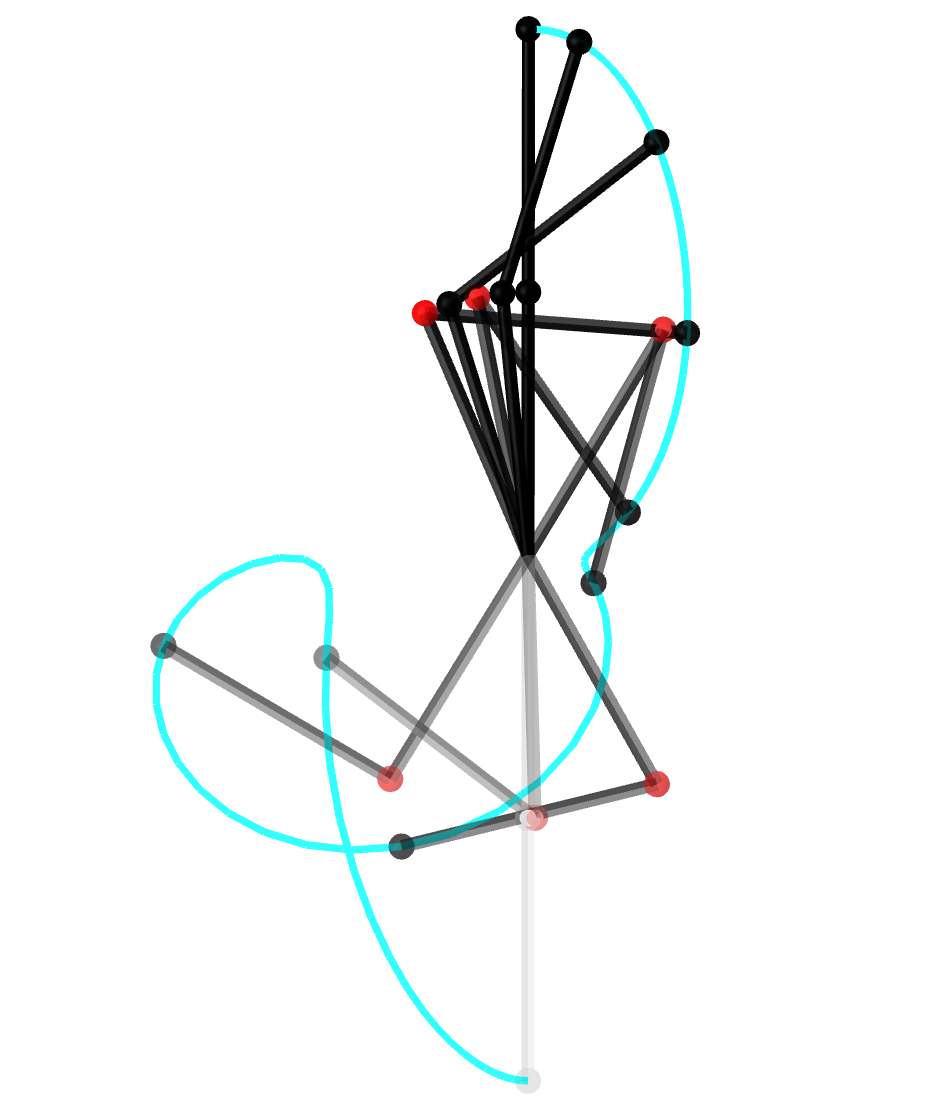
\includegraphics[width=.225\textwidth]{optimization_dynamics/acrobot_no_limits.png}
	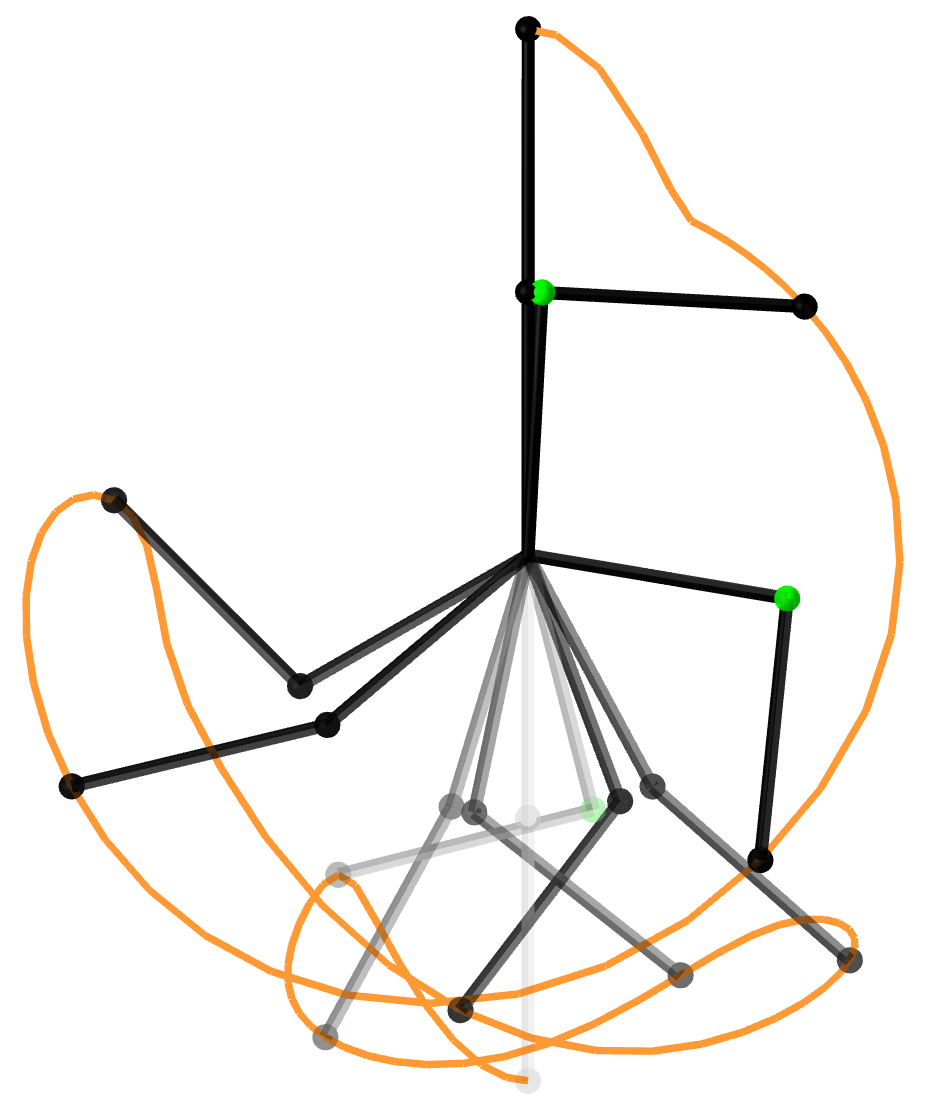
\includegraphics[width=.225\textwidth]{optimization_dynamics/acrobot_limits.png}
	\caption[Comparison of acrobot swing-up behaviors]{Optimized trajectories for acrobot systems without (left) and with (right) joint limits performing a swing-up. Red and green elbow colors indicate violation or non-violation of the joint limits, respectively.}
	\label{od_acrobot_trajectories}
\end{figure}

The unconstrained system violates joint limits, while the joint-limited system reaches the limits without exceeding them and finds a motion utilizing additional pumps. Additionally, we compare our optimization-based dynamics with the MuJoCo physics simulator and gradients provided via finite-differencing. For the unconstrained system, the optimizer is able to successfully find a swing-up trajectory. For the joint-limited system, the trajectory optimizer fails. We also note that MuJoCo is unable to enforce hard joint limits and that such constraints typically require tuning the solver parameters to produce realistic looking behavior. The results are summarized in Table \ref{od_acrobot_results}.

\begin{table}[H]
	\centering
	\caption[Numerical results for acrobot swing-up]{Comparison of objective, iterations, goal constraint violation, and solve time between MuJoCo and optimization-based dynamics with nominal and joint-limited models for acrobot. When limited, the MuJoCo model violates the joint limits and fails at the swing-up task.}
	\begin{tabular}{c c c c c}
		\toprule
		&
		\textbf{MuJoCo} &
		\textbf{MuJoCo (limited)} &
		\textbf{Ours} &
		\textbf{Ours (limited)} \\
		\toprule
		objective & 395.6 & 1.9e{6} & 48.9 & 84.2 \\
		iterations & 207  & 95 & 256 & 907 \\
		violation & 3e{-}4 & 0.2 & 5e{-}4 & 1e{-}3\\
		time (s) & 0.9 & 1.0 & 0.5 & 6.5\\
		\toprule
	\end{tabular}
	\label{od_acrobot_results}
\end{table}

\subsection{Cart-pole with Coulomb friction}

A cart-pole \cite{tedrake2014underactuated} is modeled that experiences Coulomb friction \cite{moreau2011unilateral} on both its slider and pendulum arm. We use the constraints \eqref{socp_mdp_constraints} to model stick-slip behavior.

The system has $n = 4$ states and $m = 1$ controls. We plan a swing-up trajectory for a horizon $T = 51$ and time step $h = 0.05$. The optimizer is initialized with an impulse at the first time step and zeros for the remaining initial control inputs. We compare the trajectories optimized for systems with increasing amounts of friction, see Fig. \ref{od_cartpole_state}. 

\begin{figure}[H]
	\centering
	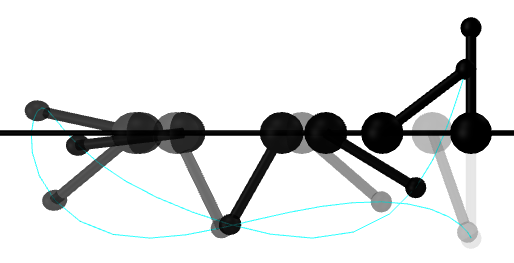
\includegraphics[width=.275\textwidth]{optimization_dynamics/cartpole_no_friction.png}
	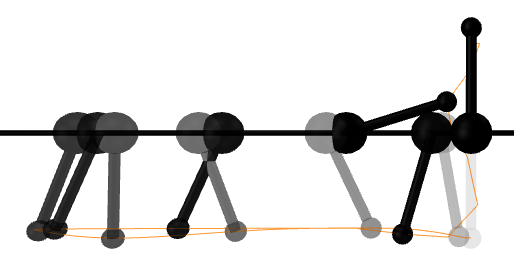
\includegraphics[width=.275\textwidth]{optimization_dynamics/cartpole_friction.png}
	\caption[Comparison of cart-pole swing-ups with friction]{Optimized trajectories for cart-pole performing a swing-up without (left, friction coefficient $=0$) and with (right, friction coefficient $=0.35$) joint friction.}
	\label{od_cartpole_state}
\end{figure}

In the presence of friction, the system performs a more aggressive maneuver at the end of the trajectory in order to achieve the swing-up. The results are summarized in Table \ref{od_cartpole_results}.

\begin{table}[H]
	\centering
	\caption[Numerical results for cart-pole swing-up with friction]{Comparison of objective, iterations, goal constraint violation, and solve time for cart-pole model with different friction coefficients.}
	\begin{tabular}{c c c c c c}
		\toprule
		\textbf{Friction} &
		\textbf{0.0} &
		\textbf{0.01} &
		\textbf{0.1} &
		\textbf{0.25} & 
		\textbf{0.35} \\
		\toprule
		objective & 5.0 & 5.5 & 11.6 & 76.3 & 163.1\\
		iterations & 456 & 485 & 406 & 472 & 943\\
		violation & 1e{-}4 & 5e{-}4 & 6e{-}4 & 1e{-}3 & 5e{-}3 \\
		time (s) & 0.36 & 2.8 & 3.1 & 4.6 & 9.8\\
		\toprule
	\end{tabular}
	\label{od_cartpole_results}
\end{table}

\subsection{Hopper gait}

We generate a gait for a Raibert hopper \cite{raibert1989dynamically}. The system's dynamics are modeled as a nonlinear complementarity problem \cite{lecleach2021fast}. The 2D system has four generalized coordinates: lateral and vertical body positions, body orientation, and leg length. There are $m = 2$ control inputs: a body moment and leg force. The state is $n = 8$, comprising the system's current and previous configurations. The  horizon is $T = 21$ with time step $h = 0.05$. The initial state is optimized and a trajectory-level periodicity constraint is employed to ensure that the first and final states, with the exception of the lateral positions, are equivalent. Finally, we initialize the solver with controls that maintain the system in an upright configuration.

We compare our implicit bi-level approach to a direct method for contact-implicit trajectory optimization \cite{manchester2020variational} that transcribes the problem and solves it with Ipopt \cite{wachter2006implementation}. We use the same models, cost functions, and comparable optimizer parameters and tolerances. 

The complexity of the classic iLQR algorithm is: $O(T m^3)$ \cite{tassa2007receding}, while a direct method for trajectory optimization that exploits the problem's temporal structure is: $O\Big(T (n^3 + n^2 m) \Big)$ \cite{wang2009fast}. The interior-point method for the dynamics generally has complexity: $O(a^3)$, although specialized solvers can reduce this cost, where $a$ is the number of primal and dual variables \cite{nocedal2006numerical}. The complexity of optimization-based dynamics and iLQR is typically dominated by the cost of the interior-point method, which is incurred at each time step in the planning horizon, so the overall complexity is $O(T a^3)$. The hopper problem has $a = 20$ and $n = 8$ and $m = 2$ with our approach. For the contact-implicit approach, the controls are augmented with contact variables, increasing the dimension to $m = 17$ at each time step. As a result, contact-implicit trajectory optimization has lower complexity in the case where a structure exploiting direct method is employed, although this is not necessarily the case when a general-purpose solver like Ipopt is called.

An optimized gait is shown in Fig. \ref{od_hopper_gait}. 

\begin{figure}[H]
	\centering
	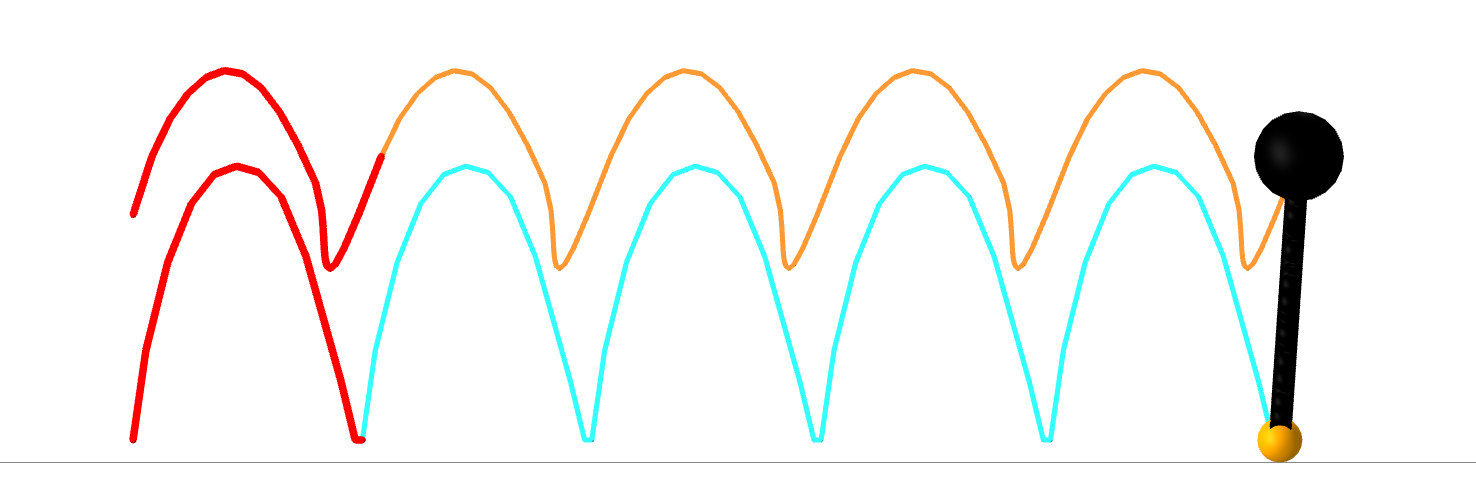
\includegraphics[width=.4\textwidth]{optimization_dynamics/hopper_gait_1.png}
	\caption[Hopper gait]{Hopper gait. Optimized template (red) for the system's body (orange) and foot (blue) trajectories is repeated to form a gait.}
	\label{od_hopper_gait}
\end{figure}

We find that our implicit approach requires fewer, but more expensive iterations, while contact-implicit trajectory optimization requires more, but less expensive iterations. Additionally, our approach more consistently returns good trajectories. Numerical comparison results are provided in Table \ref{od_hopper_bilevel_comparison}.

\begin{table}[H]
	\centering
	\caption[Numerical results for hopper gait]{Comparison between contact-implicit trajectory optimization (direct) and optimization-based dynamics + iLQR (ours) for hopper-gait examples. The objective, iterations, gait constraint violation, and solve times are compared.}
	\small
	\begin{tabular}{c c c c c c c}
		\toprule
		&
		\textbf{Direct (1)} &
		\textbf{Direct (2)} &
		\textbf{Direct (3)} &
		\textbf{Ours (1)} &
		\textbf{Ours (2)} &
		\textbf{Ours (3)} 
		\\
		\toprule
		objective & 3.5 & 20.4 & 2.9 & 3.5 & \textbf{19.8} & \textbf{2.4} \\
		iterations & 122 & 114 & 107 & \textbf{38} & \textbf{47} & \textbf{25} \\
		violation & \textbf{1\text{e-}9} & \textbf{1\text{e-}9} & \textbf{1\text{e-}9} & 3\text{e-}4 & 3\text{e-}4 & 9e{-}4\\
		time (s) & 2.0 & 2.0 & 1.8 & \textbf{0.3} & \textbf{0.4} & \textbf{0.3}\\
		\toprule
	\end{tabular}
	\label{od_hopper_bilevel_comparison}
\end{table}

\subsection{Rocket landing}

We plan a soft-landing for a rocket with 6 degrees of freedom that must transition from a horizontal to vertical orientation prior to landing while respecting thrust constraints. Unlike prior work that enforces such constraints at the optimizer level \cite{blackmore2010minimum}, we instead enforce these constraints at the dynamics level. This enables the optimizer to provide smooth controls to the dynamics, which then internally constrain the input to satisfy the system's limits at every iteration.

\begin{figure}[H]
	\centering
	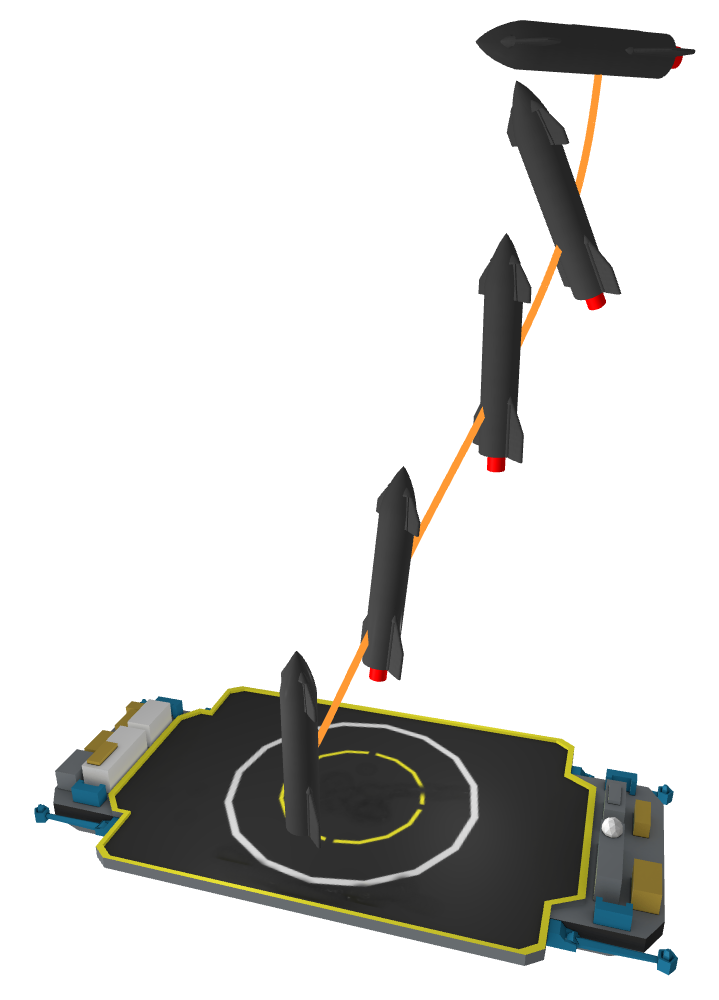
\includegraphics[width=0.2\textwidth]{optimization_dynamics/starship_ghost.png}
	\caption[Rocket belly-flop soft-landing plan]{Position trajectory (orange) for rocket performing soft landing. The system first reorients from a horizontal to vertical pose before landing with zero velocity in a target zone while respecting thrust constraints.}
	\label{od_rocket_ghost}
\end{figure}

The cone projection problem, which finds the thrust vector that is closest to the optimizer's input thrust while satisfying constraints, is formulated as:
\begin{equation}
	\begin{array}{ll}
		\underset{u}{\mbox{minimize}} & \frac{1}{2} \|u - \bar{u}\|_2^2 \\
		\mbox{subject to} & \|u_{2:3}\|_2 \leq u_1, \\
		& u_{\mbox{min}} \leq u_1 \leq u_{\mbox{max}},
	\end{array} \label{od_cone_projection}
\end{equation}
where $u, \bar{u} \in \mathbf{R}^3$ are the optimized and provided thrust vectors, respectively, $u_1$ is the component of thrust along the longitudinal axis of the rocket, $u_{\mbox{min}}$ and $u_{\mbox{max}}$ are limits on this value.

The system has $n = 12$ states and $m = 3$ controls that are first projected using (\ref{od_cone_projection}) before being applied to dynamics. The planning horizon is $T = 61$ and time step is $h = 0.05$. The controls are initialized with small random values, the initial pose is offset from the target, and the rocket has initial downward velocity. A constraint enforces the rocket's final pose, a zero velocity, vertical-orientation configuration in a landing zone.

The optimizer requires 547 iterations and takes 8.1 seconds to find a plan that successfully reorients the rocket prior to landing while respecting the thrust constraints. Without the cone constraint, the optimizer requires 521 iterations and 1.9 seconds to find a solution. However, the thrust cone constraint is violated at the first time steps. The optimized position trajectory is shown in Fig. \ref{od_rocket_ghost}.

\subsection{Planar push}
For the canonical manipulation problem of planar pushing \cite{hogan2016feedback}, we optimize the positions and forces of a robotic manipulator's circular end-effector in order to slide a planar block into an reoriented goal pose (Fig.~\ref{od_planar_push}).

\begin{figure}[H]
	\centering
	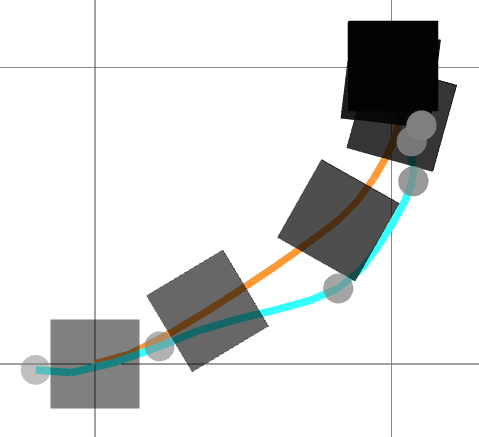
\includegraphics[width=.3\textwidth]{optimization_dynamics/planar_push_rotate_crop_2.png}
	\caption[Plan for planar-push task]{Optimized trajectories for planar-push task. The pusher (blue) and block (orange) paths are shown for a plan that maneuvers the block from a pose at the origin to a goal pose.}
	\label{od_planar_push}
\end{figure}

The system's end-effector is modeled as a fully actuated particle in 2D that can move the block (with 2D translation and orientation) via impact and friction while the two systems are in contact. The block is modeled with point friction at each of its four corners and a signed-distance function, modeled as a $p$-norm with $p=10$, is employed that enables the end-effector to push on any of the block's sides.

The system has $n = 10$ states, $m = 2$ controls, the planning horizon is $T = 26$, and the time step is $h = 0.1$. We initialize the end-effector with a control input that overcomes stiction to move the block. The block is initialized at the origin with the pusher in contact on its left side, and the block is constrained at the trajectory-level to reach a goal pose.

We compare the smooth gradients returned by differentiating through our interior-point solver with randomized smoothing to generate a zero-order gradient bundle \cite{suh2022bundled}. We use $N=100$ samples and noise sampled from a zero-mean unit Gaussian with scaling $\sigma=1.0e\mbox{-}4$. Ultimately, we find that both approaches result in similar convergence behavior of the upper-level optimizer. However, the gradient-bundle approach necessitates parallel computation of dynamics evaluations (which we do not explore in our comparison) in order to be a tractable approach, whereas the implicit-function theorem is much more efficient in a serial-computational setting. Results are provided in Table \ref{od_planarpush_results}.

\begin{table}[H]
	\centering
	\caption[Gradient comparison between implicit gradients and gradient bundles for planar-push task]{Comparison between gradients generated as zero-order gradient bundles and via the implicit-function theorem for planar-push translation (T) and rotation (R) tasks. $^*$Gradient bundles are evaluated serially.}
	\begin{tabular}{c c c c c}
		\toprule
		&
		\textbf{Bundle (T)} &
		\textbf{Bundle (R)} &
		\textbf{Implicit (T)} &
		\textbf{Implicit (R)}
		\\
		\toprule
		iterations & 18 & \textbf{32} & \textbf{17} & 33 \\
		time (s) & $+100.0^*$ & $+100.0^*$ & \textbf{8.0} & \textbf{18.3} \\
		\toprule
	\end{tabular}
	\label{od_planarpush_results}
\end{table}

\section{Limitations}\label{od_limitations}

One of the primary drawbacks to this approach is the lack of convergence guarantees for finding a solution that satisfies the dynamics representation. In practice, we find that the solver converges reliably. However, there are cases where the solver fails to meet specified tolerances. In this event we have the optimizer return the current solution and its sensitivities. We find that occasional failures like this often do not impair overall planning and that the optimizer can eventually find a dynamically feasible trajectory. Just as robust, large-scale solvers such as Ipopt \cite{wachter2006implementation} fallback to their restoration mode when numerical difficulties occur, our basic interior-point method is likely to be improved by including such a fallback routine, perhaps specific to a particular system. Additionally, we find that standard techniques such as: problem scaling, appropriate hyperparameter selection, and warm starting greatly improve the reliability of this approach.

Other potential weaknesses are the increased serial nature of the approach and cost of evaluating the dynamics and their gradients. First, iLQR is a serial algorithm, dominated by forward rollouts and backward Riccati recursions that cannot be parallelized. Similarly, the interior-point solver is a serial method dominated by a matrix factorization and back substitution that is generally not amenable to parallelization either. Second, because an iterative solver is utilized to evaluate the dynamics, calls to the dynamics are inherently more expensive compared to an explicit dynamics representation. However, such overhead can potentially be mitigated with a problem-specific solver that can exploit specialized constraints or sparsity, unlike an off-the-shelf solver's generic routines.

\section{Future Work} \label{od_future_work}
In this work we have presented a bi-level optimization framework that utilizes lower-level optimization-based dynamics for planning. This representation enables expressive dynamics by including constraint handling, internal states, and additional physical behavior modeling at the dynamics level, abstracted away from the upper-level optimizer, enabling classically unconstrained solvers to optimize motions for more complex systems.

There are numerous avenues for future work exploring optimization-based dynamics for bi-level trajectory optimization. First, in this work we explore constrained optimization problems solved with a second-order method. Another interesting problem class to consider are energy-based models \cite{lecun2006tutorial}, potentially optimized with first-order Langevin dynamics \cite{schlick2010molecular}. Second, we find that returning gradients optimized with a relaxed central-path parameter greatly improves the convergence behavior of the upper-level optimizer. An analysis of, or method for, returning gradients from the lower-level problem that best aid an upper-level optimizer would be useful. Finally, this bi-level framework could be extended to a tri-level setting where the highest-level optimizer autotunes an objective to generate model predictive control policies in an imitation-learning setting.


\chapter{Optimization with Conic and Complementarity Constraints}
\chaptermark{Conic and Complementarity Constraints}
We present a new solver for non-convex trajectory optimization problems that is specialized for robotics applications. CALIPSO, or the Conic Augmented Lagrangian Interior-Point SOlver, combines several strategies for constrained numerical optimization to natively handle second-order cones and complementarity constraints. It reliably solves challenging motion-planning problems that include contact-implicit formulations of impacts and Coulomb friction and state-triggered constraints where general-purpose non-convex solvers like SNOPT and Ipopt fail to converge. Additionally, CALIPSO supports efficient differentiation of solutions with respect to problem data, enabling bi-level optimization applications like auto-tuning of feedback policies. Reliable convergence of the solver is demonstrated on a range of problems from manipulation, locomotion, and aerospace domains. An open-source implementation of this solver is available.

\vspace*{\fill}

\noindent CALIPSO: A Differentiable Solver for Trajectory Optimization with Conic and Complementarity Constraints. Taylor A. Howell, Kevin Tracy, Simon Le Cleac'h, and Zachary Manchester. International Symposium of Robotic Research. 2022.

\pagebreak 

\section{Introduction}
Trajectory optimization is a powerful tool for offline generation of complex behaviors for dynamic systems, as well as online as a planner or feedback controller within model predictive control frameworks.  The use of constraints greatly enhances the ability of a designer to generate desirable solutions, enforce safe behaviors, and model physical phenomena. Unfortunately, many constraint types that have important and direct applications to robotics are poorly handled by existing general-purpose non-convex solvers \cite{nocedal2006numerical} or differential dynamic programming (DDP) algorithms \cite{jacobson1970differential}. 

Second-order cones \cite{boyd2004convex}, which commonly appear as friction-cone \cite{moreau2011unilateral} or thrust-limit \cite{blackmore2010minimum} constraints, present difficulties for these solvers due to their nondifferentiability at commonly occurring states, like when the friction or thrust forces are zero. Common reformulations of these constraints for solvers like SNOPT \cite{gill2005snopt} and Ipopt \cite{wachter2006implementation} are typically non-convex and fail to work well in practice \cite{vanderbei1998using}.

Contact dynamics, including impact and friction, are naturally modeled with complementarity constraints \cite{scheel2000mathematical}. This formulation constrains contact forces to only take on non-zero values when the distance between objects is zero. State-triggered constraints \cite{szmuk2019real}, in which constraints switch on or off in different regions of the state space, can similarly be modeled with complementarity constraints. However, these constraints violate the linear independence constraint qualification (LICQ), a fundamental assumption in the convergence theory of standard second-order solvers \cite{nocedal2006numerical, biegler2010nonlinear}.

In this work, we present a new solver for trajectory optimization, CALIPSO: Conic Augmented Lagrangian Interior-Point SOlver. The development of this solver is motivated by challenging non-convex motion-planning problems that require second-order cone and complementarity constraints; in particular, contact-implicit trajectory optimization \cite{posa2014direct, manchester2020variational} for locomotion and manipulation. CALIPSO combines a number of ideas and algorithms from constrained numerical optimization to solve these difficult problems reliably. 

Second-order cones are handled using an interior-point method \cite{vandenberghe2010cvxopt} that exploits the convexity of these constraints for strict enforcement without the need for linear approximations. All equality constraints are handled using an augmented Lagrangian method \cite{bertsekas2014constrained}, which does not require the constraints to satisfy LICQ and is robust to the degeneracies that can arise from complementarity constraints \cite{izmailov2012global}. Additionally, both the interior-point and augmented-Lagrangian methods are formulated in a primal-dual fashion to enhance the numerical robustness and performance of the solver. The computation of Newton steps on the combined primal-dual augmented-Lagrangian and interior-point KKT conditions are reformulated as a symmetric linear system to enable the use of fast, direct linear algebra methods \cite{davis2005algorithm}. Finally, the implicit-function theorem \cite{dini1907lezioni,amos2017optnet} is utilized to efficiently differentiate through solutions, enabling bi-level optimization applications such as auto-tuning of model predictive control policies.

Our specific contributions are:
\begin{itemize} 
	\item A differentiable trajectory optimization solver with native support for second-order cones and reliable handling of complementarity constraints
	\item A novel, combined, interior-point and augmented-Lagrangian algorithm for non-convex optimization
	\item A symmetric reformulation of the combined method's KKT system for fast symmetric linear-system solvers
	\item A collection of benchmark robot motion-planning problems that contain second-order cone and complementarity constraints
	\item An open-source implementation of the solver written in Julia
\end{itemize}

In the remainder of this chapter, we first provide an overview of related work on trajectory optimization methods in Section \ref{calipso_related_work}. Then, we provide the necessary background on complementarity constraints and LICQ in Section \ref{calipso_background}. Next, we present CALIPSO and its key algorithms and routines in Section \ref{calipso}. We then demonstrate CALIPSO on a collection of robot motion-planning examples in Section \ref{calipso_results}. Finally, we conclude with a discussion of limitations in Section \ref{calipso_limitations} and future work in Section \ref{calipso_future_work}.

\section{Related work} \label{calipso_related_work}

Trajectory optimization problems are solved with methods that are classically categorized as either indirect or direct \cite{betts1998survey}. Indirect methods include shooting methods, DDP \cite{jacobson1970differential}, and iterative LQR (iLQR) \cite{li2004iterative}. These methods exploit the temporal structure of the problem and utilize a Riccati backward pass to compute updates for control variables followed by forward simulation rollouts to update the states. Classically, apart from the dynamics, these methods do not include support for constraints. In recent years, various approaches have extended these methods to handle constraints \cite{tassa2014control,howell2019altro, howell2022trajectory,mastalli2020crocoddyl,singh2022optimizing,jallet2022constrained,jackson2021altro}. However, reliable constraint handling and solution accuracy for these methods is still challenging in many scenarios.

Direct methods, in contrast, directly transcribe the trajectory optimization problem as a constrained non-convex problems, with both states and controls as decision variables \cite{stryk1993numerical}. The transcription is provided to a general-purpose solver such as SNOPT or Ipopt. This approach is generally reliable and enables robust constraint handling. However, these solvers do not exploit the temporal structure of the trajectory optimization problem like indirect methods, and historically have been thought to converge to solutions more slowly as a result. To address this limitation, direct solvers tailored for the underlying trajectory optimization problem structure have been proposed \cite{wang2009fast} and are available as commercial tools \cite{zanelli2020forces}. 

While providing reliable constraint handling for equality and inequality constraints in many scenarios, direct methods lack support for second-order cones \cite{boyd2004convex} and exhibit difficulties handling complementarity constraints \cite{scheel2000mathematical}. The exact handling of second-order cones as inequality constraints with these solvers results in poor practical performance because the nondifferentiable point of the cone is frequently visited in robotics applications (e.g., an object resting on a surface with zero friction force). Classic reformulations are non-convex and similarly exhibit poor and unreliable convergence \cite{vanderbei1998using}. Recently, sequential convexification approaches have been developed that are able to handle second-order cones by iteratively solving convex approximations of the original problem using general-purpose cone solvers \cite{szmuk2020successive,bonalli2019gusto}. 

The complementarity constraints that can arise in robotics problems are generally difficult for solvers to handle because they are non-convex and violate LICQ. To overcome this, a number of problem reformulations and constraint relaxation techniques have been proposed and explored for interior-point \cite{biegler2010nonlinear,raghunathan2003mathematical} and augmented Lagrangian \cite{izmailov2012global} methods, but these approaches largely remain \textit{ad hoc} and are unavailable in state-of-the-art solvers for trajectory optimization, which we compare in Table \ref{calipso_trajopt_solvers}.

\begin{table}[H]
	\centering
	\caption[Comparison of optimizers]{Comparison of general-purpose and trajectory optimization solvers.}
	\scriptsize
	\begin{tabular}{c c c c c c}
		\toprule
		\textbf{Solver} &
		\textbf{Method} &
		\textbf{Accuracy} &
		\textbf{Second-Order} &
		\textbf{Complementarity} &
		\textbf{Differentiable} \\
		\toprule
		Ipopt \cite{wachter2006implementation} & direct & high & \ding{53} & \ding{53} & \ding{53} \\
		SNOPT \cite{gill2005snopt} & direct & high & \ding{53} & \ding{53} & \ding{53} \\
		CVX \cite{agrawal2019differentiable} & direct & high & \checkmark & \ding{53} & \checkmark \\
		\toprule
		ALTRO \cite{howell2019altro} & indirect & medium & \checkmark & \ding{53} & \ding{53} \\
		Trajax \cite{trajax} & indirect & medium & \ding{53} & \ding{53}  & \checkmark \\
		GuSTO \cite{bonalli2019gusto} & direct & high & \checkmark & \ding{53} & \ding{53} \\
		FORCES \cite{zanelli2020forces} & direct & high & \ding{53} & \ding{53} & \ding{53} \\
		Drake \cite{drake} & direct & high & \ding{53} & \ding{53} & \ding{53} \\
		\toprule
		CALIPSO & direct & high & \checkmark & \checkmark & \checkmark \\
		\toprule
	\end{tabular}
	\label{calipso_trajopt_solvers}
\end{table}

\section{Background} \label{calipso_background}
In this section, we provide background on complementarity constraints and LICQ.

\subsection{Complementarity constraints}
Contact-implicit trajectory optimization \cite{posa2014direct} optimizes trajectories for systems that make and break contact with their environments and represents dynamics using complementarity constraints. For example, optimizing motion over a single time step for an actuated particle in a single dimension, resting on a surface, modeled with impact such that it cannot pass through the floor:
\begin{equation}
	\begin{array}{ll}
		\underset{z, u, \gamma}{\mbox{minimize }} & \frac{1}{2}(z - z_{\mbox{g}})^2 + \frac{1}{2}u^2 \\
		\mbox{subject to } & m \big(z / h + g h \big) = \gamma + u, \\
		& z \cdot \gamma = 0, \\
		& z, \gamma \geq 0,
	\end{array} \label{calipso_ci_trajopt}
\end{equation}
with position $z\in \mathbf{R}$, control input $u \in \mathbf{R}$, contact impulse $\gamma \in \mathbf{R}$, mass $m \in \mathbf{R}_{++}$, gravity $g \in \mathbf{R}_{+}$, time step $h \in \mathbf{R}_+$, and goal $z_{\mbox{g}} \in \mathbf{R}$. These constraints are derived from a constrained discrete Lagrangian \cite{manchester2020variational}. The set of constraints on $z$ and $\gamma$ are collectively referred to as a complimentary constraint, and are sometimes abbreviated $z \perp \gamma$. This formulation does not require pre-specified contact-mode sequences or hybrid dynamics since the solver is able to optimize physically correct contact dynamics at each time step.

\subsection{Linear independence constraint qualification}
General-purpose second-order solvers that rely on Newton's method to compute search directions (e.g., SNOPT and Ipopt) assume that the constraints provided by the user satisfy the LICQ in the neighborhood of solutions. Certain classes of constraints, including complementarity conditions that naturally arise in contact dynamics, often do not satisfy this assumption. 
We demonstrate how this assumption is violated with a simple contact-implicit trajectory optimization problem \eqref{calipso_ci_trajopt}. The Lagrangian for the problem is: 
\begin{equation}
	L(z, u, \gamma, a, b, c, d) = \frac{1}{2}(z - z_{\mbox{g}})^2 + \frac{1}{2}u^2 + a \big( m (z / h + g h ) - \gamma - u \big) + b z \gamma - c z - d \gamma,
\end{equation}
where $a, b, c, d \in \mathbf{R}$ are the Lagrange multipliers, or ``dual variables,'' associated with constraints. The KKT system is:

\begin{equation} 
	\setstackgap{L}{1.1\baselineskip}
	\fixTABwidth{T}
	\bracketMatrixstack{
		1 & b & 0 & m / h & \gamma & -1 & 0 \\
		b & 0 & 0 & 1 & z & 0 & -1 \\
		0 & 0 & 1 & -1 & 0 & 0 & 0 \\
		m / h & -1 & -1 & 0 & 0 & 0 & 0 \\
		\gamma & z & 0 & 0 & 0 & 0 & 0 \\
		c & 0 & 0 & 0 & 0 & z & 0 \\ 
		0 & d & 0 & 0 & 0 & 0 & \gamma
	}
	\bracketMatrixstack{
		\Delta z\\
		\Delta \gamma \\
		\Delta u \\
		\Delta a \\
		\Delta b \\
		\Delta c \\
		\Delta d
	}
	=
	-
	\bracketMatrixstack{
		(z - z_{\text{g}}) + a m / h + b \gamma - c \\ 
		a + b z - d \\
		u - a \\ 
		m \big(z / h + g h \big) - \gamma - u \\
		z \cdot \gamma \\ 
		c \cdot z \\ 
		d \cdot \gamma 
	}, 
	% \notag \\
	% z, \gamma, c, d & \geq 0,
	\label{calipso_licq_kkt}
\end{equation}
\begin{equation}
	z, \gamma, c, d, \geq 0,
\end{equation}
with first-order necessary (KKT) conditions (right-hand side) and KKT matrix (left-hand side). The Newton step that a standard second-order solver would take to drive these KKT conditions to zero is computed by solving this system \eqref{calipso_licq_kkt}.

In the scenario where the particle is above the surface (i.e., $z > 0$) the contact impulse must be zero (i.e., $\gamma = 0$). As a result, the fifth and seventh rows of the KKT matrix will be linearly dependent, resulting in non-unique optimal dual variables and violation of LICQ. A similar result occurs when $\gamma > 0$ and $z = 0$. Consequently, the Newton step is not well defined in these cases, causing difficulties for the solver. While a myriad of \textit{ad hoc} heuristics exist to alleviate this problem, we pursue a more rigorous approach in the following sections based on ideas from constrained numerical optimization.

\begin{figure}[H]
	\centering
	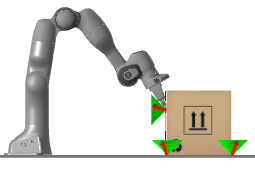
\includegraphics[width=.3\textwidth]{calipso/push_cones.png}
	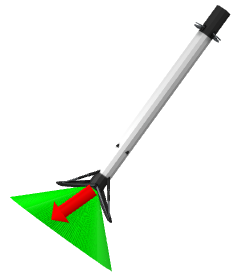
\includegraphics[width=.175\textwidth]{calipso/rocket_cone.png}
	\caption[Robotics applications with conic and complementarity constraints]{Robotics applications with second-order cone constraints include Coulomb friction at contact points in manipulation tasks (left) and thrust limits on rockets (right). Cone constraints are shown in green, while force vectors are shown in red.}
	\label{calipso_second_order_cone_robots}
\end{figure}

\section{CALIPSO} \label{calipso}
CALIPSO is a differentiable primal-dual augmented Lagrangian interior-point solver for non-convex optimization problems with second-order cone and complementarity constraints. Its standard problem formulation is:
\begin{equation}
	\begin{array}{ll}
		\underset{x}{\mbox{minimize }}  & c(x; \theta) \\
		\mbox{subject to } & g(x; \theta) = 0, \\
		& h(x; \theta) \in \mathcal{K},
	\end{array}
	\label{calipso_problem}
\end{equation}
with decision variables $x \in \mathbf{R}^n$, problem data $\theta \in \mathbf{R}^d$, equality constraints $g : \mathbf{R}^n \times \mathbf{R}^d \rightarrow \mathbf{R}^m$, and constraints $h : \mathbf{R}^n \times \mathbf{R}^d \rightarrow \mathbf{R}^p$ in cone $\mathcal{K} = \mathbf{R}_{++}^q \times Q_{l_1}^{(1)} \times \dots \times Q_{l_j}^{(j)}$ comprising a $q$-dimensional inequality and $j$ second-order cones, each of dimension $l_i$. Internally, problem \eqref{calipso_problem} is reformulated and additional slack variables $r \in \mathbf{R}^m$ and $s \in \mathbf{R}^p$, associated with the equality and cone constraints, respectively, are introduced, and the following modified problem is formed:
\begin{equation}
	\begin{array}{ll}
		\underset{x, r, s}{\mbox{minimize }}  & c(x; \theta) + \lambda^T r + \frac{\rho}{2} r^T r - \kappa \sum \limits_{i = 1}^p \mbox{log}(s^{(i)}) \\
		\mbox{subject to } & g(x; \theta) - r  =0, \\
		& h(x; \theta) - s = 0, \\
		& s \in \mathcal{K},
	\end{array}
	\label{calipso_internal_problem}
\end{equation}
The modified problem's Lagrangian is:
\begin{multline} 
	L(w; \theta, \lambda, \rho, \kappa) = c(x; \theta) + y^T (g(x; \theta) - r) + z^T (h(x; \theta) - s) \\
	+ \lambda^T r + \frac{\rho}{2} r^T r - \kappa \sum \limits_{i = 1}^p \mbox{log}(s^{(i)}). \label{calipso_lagrangian}
\end{multline}
For convenience we denote the concatenation of all of the solver's variables as $w = (x, r, s, y, z, t)$. The KKT system is:
\begin{align} 
	\begin{bmatrix} 
		L_{xx} + \epsilon_p I & 0      & 0 & g_x^T & h_x^T &  0 \\ 
		0      & (\rho + \epsilon_p) I & 0 &    -I &    0 &  0 \\ 
		0      & 0      & \epsilon_p I &    0 &   -I & -I \\ 
		g_x    & -I     & 0 &    -\epsilon_d I &    0 &  0 \\ 
		h_x    & 0      & -I & 0  & -\epsilon_d I & 0 \\
		0 & 0 & P_s & 0 & 0 & P_t - \epsilon_d I
	\end{bmatrix}
	\begin{bmatrix}
		\Delta x \\ 
		\Delta r \\ 
		\Delta s \\ 
		\Delta y \\ 
		\Delta z \\ 
		\Delta t
	\end{bmatrix} \label{calipso_kkt}
	&= 
	- 
	\begin{bmatrix} 
		c_x + g_x^T y + h_x^T z \\ 
		\lambda + \rho r - y \\ 
		-z - t \\ 
		g - r \\ 
		h - s \\
		s \circ t - \kappa \mathbf{e}
	\end{bmatrix}, \notag \\
	J \Delta w &= - R,
\end{align}
where and $P_s, P_t \in \mathbf{S}^p$ are the cone-product Jacobians, and $\epsilon_p, \epsilon_d \in \mathbf{R}_+$ are additional primal and dual regularization terms, respectively.

\subsection{Search direction}
The nominal KKT system \eqref{calipso_kkt} without regularization (i.e., $\epsilon_p, \epsilon_d = 0$) is non-symmetric, potentially with undesirable eigenvalues that will not return a descent direction. The solver modifies this system for faster computation and a more reliable search direction.

\paragraph{Symmetric KKT system.}
To be amenable to fast solvers for symmetric linear systems, the nominal KKT system is reformulated:
\begin{align} 
	\begin{bmatrix} 
		L_{xx} + \epsilon_p I & g_x^T & h_x^T \\ 
		g_x & -\Big(\frac{1}{\rho + \epsilon_p} I \Big) & 0 \\ 
		h_x & 0 & -\Big(\epsilon_d I + ((P_s + \epsilon_p \bar{P}_t)^{-1} \bar{P}_t) \Big)
	\end{bmatrix} 
	\begin{bmatrix} 
		\Delta x \\ 
		\Delta y \\ 
		\Delta z \\
	\end{bmatrix} 
	&=
	-\begin{bmatrix} 
		L_x \\ 
		\bar{L}_y\\ 
		\bar{L}_z \\
	\end{bmatrix}, \label{calipso_search_direction_xyz}
\end{align} 
using Schur complements \cite{boyd2004convex}, where $\bar{L}_y = L_y + \frac{1}{\rho + \epsilon_p} L_r$, $\bar{L}_z = L_z + (P_s + \epsilon_p \bar{P}_t)^{-1}(\bar{P}_t L_s + L_t)$, and $\bar{P}_t = P_t - \epsilon_d I$. The remaining search directions:
\begin{align} 
	\Delta r &= (\Delta y + L_r) / (\rho + \epsilon_p), \label{calipso_search_direction_r}\\
	\Delta s &= (P_s + \epsilon_p \bar{P}_t)^{-1} (\bar{P}_t \Delta z + \bar{P}_t L_s + L_r), \label{calipso_search_direction_s}\\
	\Delta t &= - \Delta z + \epsilon_p \Delta s - L_s, \label{calipso_search_direction_t}
\end{align}
are recovered from the solution \eqref{calipso_search_direction_xyz}. 
Iterative refinement \cite{nocedal2006numerical} is performed to improve the quality of the search directions computed using the symmetric system (\ref{calipso_search_direction_xyz} - \ref{calipso_search_direction_t}).

\paragraph{Inertia correction.}
To ensure a unique descent direction, the left-hand side of the symmetric KKT system \eqref{calipso_search_direction_xyz} is corrected to have an inertia of $n$ positive, $m + p$, negative, and no zero-valued eigenvalues. This is accomplished via adaptive regularization that increases the regularization terms, and subsequently reduces the values when possible to limit unnecessary corrections, using a heuristic developed for Ipopt \cite{wachter2006implementation}.

\subsection{Line search}
Cone variables are initialized being strictly feasible at the start of each solve. A filter line search that is a slight modification of the one used by Ipopt \cite{wachter2006implementation} is performed to ensure an improvement to the solution is achieved at each step of the algorithm and step sizes are initially chosen using a fraction-to-the-boundary rule to ensure that the cone constraints remain strictly satisfied. Additionally, a separate step size is computed for the candidate cone dual variables $t$ to avoid unnecessarily restricting progress of the remaining variables.

After satisfying the cone constraints, a filter line search is performed with the merit function:
\begin{equation}
	\varphi(x, r, s; \theta, \lambda, \rho, \kappa) = c(x; \theta) + \lambda^T r + \frac{\rho}{2} r^T r - \kappa \sum \limits_{i = 1}^p \mbox{log}(s^{(i)}), \label{calipso_merit}
\end{equation}
and violation metric:
\begin{equation} 
	\eta = \|(g(x) - r, h(x) - s) \|_1 / (m + p). \label{slack_constraint_violation}
\end{equation}
The step size is further decremented until either the merit or violation metric is decreased \cite{wachter2005line}. A filter: 
\begin{equation}
\mathcal{F} = \{(\varphi^{(1)}, \eta^{(1)}), \dots, (\varphi^{(p)}, \eta^{(p)})\},
\end{equation}
comprises a set of $p$ previously accepted points. 
A candidate point must satisfy:
\begin{equation} 
  \hat{\varphi} < \varphi^{(i)} \, \lor \, \hat{\eta} < \eta^{(i)}, \quad i = 1, \dots, v,
\end{equation}
for each previous point in the filter. Then, the Armijo condition \cite{nocedal2006numerical}:
\begin{equation} 
  \hat{\varphi} < \varphi + \epsilon_a \alpha ( \varphi_x^T \Delta x + \varphi_r^T \Delta r + \varphi_s^T \Delta s), \label{calipso_armijo}
\end{equation}
with tolerance $\epsilon_a \in \mathbf{R}_+$, must be satisfied in order to accept a candidate point. Finally, the filter is augmented with the candidate point:
\begin{equation} 
  \mathcal{F} \leftarrow \mathcal{F} \cup (\hat{\varphi}, \hat{\eta}).
\end{equation}

\subsection{Cone-product Jacobians} \label{calipso_cone_product_jacobians}
The cone-product Jacobian's $P_s$ and $P_t$ have known structure and decompose by cone. This enables fast matrix products and inverses. For inequalities: 
\begin{equation} 
	P_a(a, b) = \mbox{\textbf{diag}}(b), \quad P_a(a, b)^{-1} = \mbox{\textbf{diag}}(1 / b_1, \dots, 1 / b_q),
\end{equation} 
are diagonal matrices. For second-order cones:
\begin{equation} 
	P_a(a, b) = \begin{bmatrix} b^{(1)} & (b^{(2:l)})^T \\ b^{(2:l)} & b^{(1)} I \end{bmatrix},
\end{equation} 
is an arrowhead matrix and its inverse has complexity linear in the dimension of the matrix \cite{najafi2014efficient}.

\subsection{Fraction-to-the-boundary} \label{calipso_f2b} 
Step sizes $\alpha$ for cone-variable updates are selected to ensure that the fraction-to-the-boundary rule \cite{wachter2006implementation}:
\begin{align}
	s + \alpha \Delta s - (1 - \tau) s \in \mathcal{K}, \label{calipso_fraction_to_boundary}
\end{align}
is satisfied for a cone. The parameter $\tau \in [0, 1]$ helps prevent cone variables from reaching their respective boundaries too quickly and is increased during outer updates. The fraction-to-the-boundary value is increased during each outer update.

\subsection{Iterative refinement} \label{calipso_iterative_refinement_appendix}
A drawback to computing search directions using the symmetric system is the potential worsening of the numerical conditioning of the system. As a result, the error:
\begin{equation} 
	e = R + J \Delta w, \label{calipso_search_direction_error}
\end{equation}
will be nonzero. To account for this, we correct the search direction by performing iterative refinement \cite{nocedal2006numerical}. A linear system:
\begin{equation}
	J \Delta e = -e,
\end{equation}
is solved using the error as the residual in order to compute a correction $\Delta e$. This correction is then utilized to update the search direction:
\begin{equation} 
	\Delta w \leftarrow \Delta w + \Delta e. \label{calipso_search_direction_correction}
\end{equation}
This procedure (\ref{calipso_search_direction_error} - \ref{calipso_search_direction_correction}) is repeated until the norm of the error is below a desired tolerance. 

In the case where iterative refinement fails (e.g., exceeding the solver's maximum number of refinement iterations), new candidate points are evaluated using an alternative search direction computed using the regularized non-symmetric system and an LU factorization.

\subsection{Outer updates}
Convergence of a subproblem \eqref{calipso_internal_problem} occurs for fixed values of $\lambda$, $\rho$, and $\kappa$, when the criteria: $\| R \|_{\infty} \leq \gamma_{\kappa} \kappa$,
is met for $\gamma_{\kappa} \in \mathbf{R}_+$. This criteria does not require strict satisfaction of subproblems and decreases the total number of iterations required by the solver. Outer updates on the central-path parameter and the penalty value are subsequently performed:
\begin{equation}
	\kappa \leftarrow  \mbox{max}\Big(\kappa_{\mbox{min}}, \mbox{min}(\psi_{\kappa} \cdot \kappa, \kappa^{\zeta_{\kappa}})\Big), \quad
	\rho \leftarrow \mbox{min}\Big(\rho_{\mbox{max}}, \mbox{max}(\phi_{\rho} \cdot \rho, 1 / \kappa) \Big). \label{calipso_outer_update}
\end{equation}
The updates are clipped to prevent unnecessarily small/large values.

\subsection{Initialization}

Given an initial guess for the primal variables $x_{\mbox{init}}$, the solver's variables are initialized with:
\begin{equation} 
  r = g(x_{\mbox{init}}), \,
  s_{\mbox{ineq}} = \mathbf{1}_q, \,
  s_{\mbox{so}}^{(i)} = (1, 1 / 10 \cdot \mathbf{1}_{l-1}), \,
  y = 0_m, \,
  z = 0_p, \,
  t = s, \label{calipso_initialize}
\end{equation}
where $s_{\mbox{ineq}}$ and $s_{\mbox{so}}$ are inequality and second-order variables, respectively, and are initialized strictly feasible. While more complex schemes may be effective, particularly for specific problems, this simple initialization works well in practice as a default setting.

\begin{algorithm}[H]
	\caption{CALIPSO}\label{calipso_algorithm}
	\begin{algorithmic}[H]
		\Procedure{Optimize}{$x, \theta, c, g, h, \mathcal{K}, \gamma$}
		\State \textbf{Parameters}: $\kappa = 1, \rho = 1, \lambda = 0$
		\State \textbf{Initialize}: $r, s, y, z, t$
		\State \textbf{Until} $\| R(w; \theta, y, \infty, 0) \|_{\infty} < \gamma_R$
		\State \indent \textbf{Until} $\|R(w; \theta, \lambda, \rho, \kappa)\|_{\infty} < \gamma_{\kappa} \kappa$ \textbf{do}
		\State \indent \indent $\mathbf{inertia}$ $\mathbf{correction}$: $\epsilon_p$, $\epsilon_d$ \Comment{Eq. (\ref{calipso_kkt})}
		\State \indent \indent $\mathbf{search}$ $\mathbf{direction}$: $\Delta w = (\Delta x, \Delta r, \Delta s, \Delta y, \Delta z, \Delta t)$ \Comment{Eqs. (\ref{calipso_search_direction_xyz} - \ref{calipso_search_direction_t})}
		\State \indent \indent $\mathbf{cone}$ $\mathbf{line}$ $\mathbf{search}$: $\alpha$, $\alpha_t$
		\State \indent \indent $\mathbf{candidate}$: $\hat{x} = x + \alpha \Delta x$, $\hat{r} = r + \alpha \Delta r$, $\hat{s} = s + \alpha \Delta s$
		\State \indent \indent $\mathbf{filter}$: $\hat{\varphi}$, $\hat{\eta}$
		\State \indent \indent $\mathbf{update}$: $w \leftarrow (\hat{x}, \hat{r}, \hat{s}, y + \alpha \Delta y, z + \alpha \Delta z, t + \alpha_t t)$
		\State \indent $\mathbf{outer}$ $\mathbf{update}$: $\lambda, \rho, \kappa$ \Comment{Eq. (\ref{calipso_outer_update}, \ref{intro_augmented_lagrangian_update})}
		\State $\mathbf{Differentiate}$: $\partial w / \partial \theta$ \Comment{Eq. \ref{intro_solution_sensitivity}}
		\State \textbf{Return} $w, \partial w / \partial \theta$
		\EndProcedure
	\end{algorithmic}
\end{algorithm}

\subsection{Solution derivatives}
The solution $w^*(\theta)$ returned by CALIPSO is differentiable with respect to its problem data $\theta$. At a solution point, the residual is approximately zero \eqref{intro_implicit_function}, and sensitivities \eqref{intro_solution_sensitivity} are computed using $\partial R / \partial w = J$, which has already been computed and factorized, and:
\begin{equation} 
	\partial R / \partial \theta = (
	L_{x\theta}, 
	0_{m \times d}, 
	0_{p \times d},
	g_{\theta},
	h_{\theta},
	0_{p \times d}).
\end{equation}
Additionally, the sensitivity of the solution with respect to each element of the problem data can be computed in parallel.

\subsection{Implementation}
The CALIPSO solver is summarized in Algorithm \ref{calipso_algorithm}. An open-source implementation of the solver, \texttt{CALIPSO.jl}, written in Julia, is provided. The solver, and the following examples, are available at: 
\begin{center}
	\url{https://github.com/thowell/CALIPSO.jl}. 
\end{center}

Transcribing problems for CALIPSO requires specifying the objective and constraint functions, and the number of primal variables. Trajectory-optimization problems are automatically formulated into the standard form \eqref{calipso_problem}. Gradients and sparse Jacobians are generated symbolically using the Julia package \texttt{Symbolics.jl}.

\section{Results} \label{calipso_results}
We highlight the capabilities of CALIPSO by optimizing a collection of motion-planning problems from manipulation, locomotion, and aerospace domains that require second-order cone and complementarity constraints while transcribing constraints without approximation. Next, we demonstrate the ability to differentiate through the solver and auto-tune policies for non-convex underactuated robotic systems. Additional details about the experimental setups are available in the open-source implementation. A collection of non-convex problems are provided in the Appendix.

\subsection{Contact-implicit trajectory optimization}

CALIPSO is utilized to optimize contact-implicit trajectory optimization problems \eqref{intro_ci_trajopt}. The contact dynamics \cite{posa2014direct} are directly transcribed without modification. Comparisons are performed with Ipopt using the default MUMPS linear-system solver, and results are summarized in Table \ref{calipso_contact_implicit_trajopt_comparison}.

\begin{figure}[H]
	\centering
	\captionsetup[subfigure]{justification=centering}
	\begin{subfigure}{.495\textwidth}
		\centering
		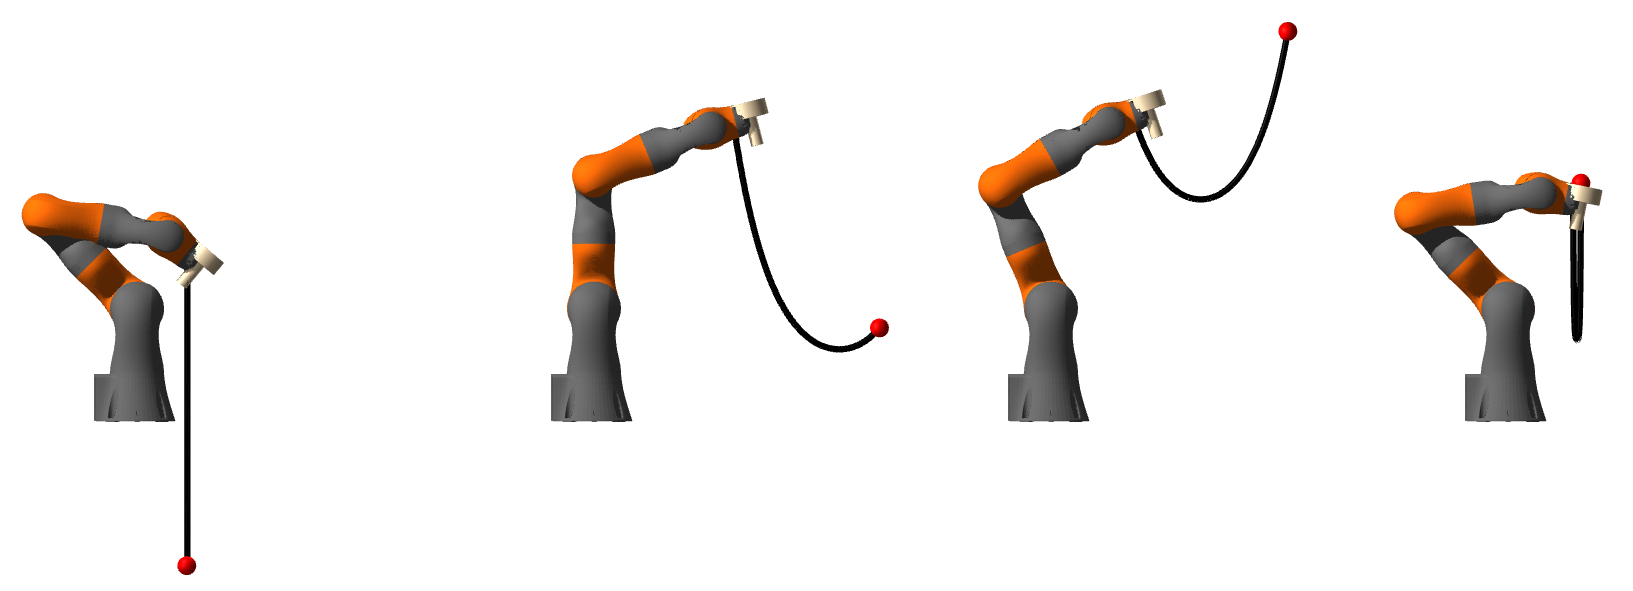
\includegraphics[height=2.5cm]{calipso/ballincupstack.png}
		\caption{ball-in-cup}
		\label{calipso_ci_ballincup}
	\end{subfigure}%
	\begin{subfigure}{.495\textwidth}
		\centering
		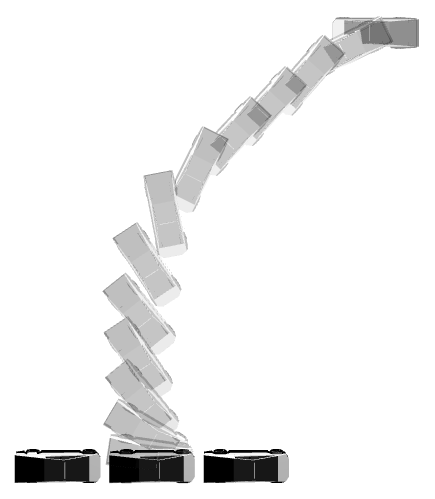
\includegraphics[height=2.5cm]{calipso/cyberdrift_calipso.png}
		\caption{drifting}
		\label{calipso_ci_drifting}
	\end{subfigure}
	\vskip\baselineskip
	\begin{subfigure}{.495\textwidth}
		\centering
		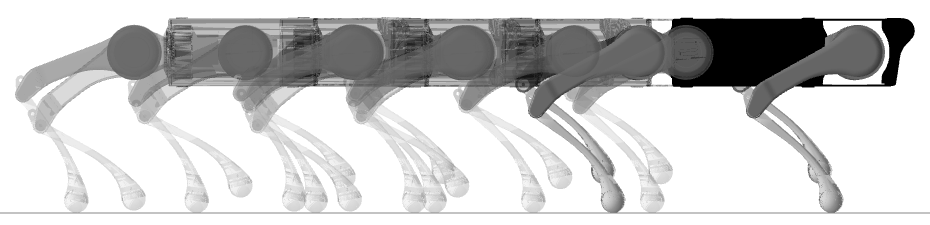
\includegraphics[height=1.25cm]{calipso/quadruped_calipso.png}
		\caption{quadruped gait}
		\label{calipso_ci_quadruped_gait}
	\end{subfigure}
	\begin{subfigure}{.495\textwidth}
		\centering
		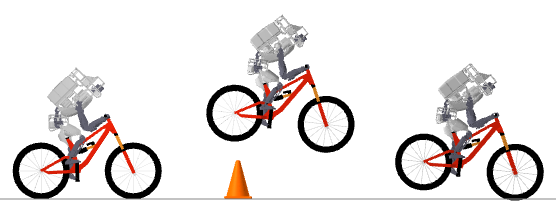
\includegraphics[height=1.25cm]{calipso/atlas_bunnyhop_stack.png}
		\caption{bunny-hop}
		\label{calipso_ci_bunnyhop}
	\end{subfigure}
	\caption[Contact-implicit trajectory optimization examples]{Contact-implicit trajectory optimization examples optimized with CALIPSO. (a) Ball attached to a string is swung into a cup by optimizing end-effector positions and forces. (b) Autonomous car plans a drifting maneuver in order to parallel park. (c) Gait for a quadruped is optimized via a single step and loop constraint. (d) Bicycle robot performs a bunny hop over an obstacle to reach a goal state.}
	\label{calipso_ci_examples}
\end{figure}

\paragraph{Ball-in-cup.} The position and applied forces of a robotic manipulator's end-effector are optimized to swing a ball into a cup (Fig. \ref{calipso_ci_ballincup}). A string between the end-effector and ball is modeled with inequality and complementarity constraints. CALIPSO finds a physically realistic motion plan that is verified with inverse kinematics in simulation, while the Ipopt solution is of poor quality and violates physics by applying nonnegligible force to the ball while the string is slack.

\paragraph{Drifting.}
A parallel-park maneuver is planned that requires an autonomous vehicle to drift (i.e., plan a trajectory with both sticking and sliding contact) into a goal configuration between two parked vehicles (Fig. \ref{calipso_ci_drifting}). The system is modeled as a Dubins car \cite{lavalle2006planning} with Coulomb friction applied to the wheels. Ipopt exhibits extremely poor converge and violates the friction cones to solve this problem, whereas CALIPSO finds a high-quality solution that leverages the nonlinear friction cone to slide into the narrow parking spot.

\paragraph{Quadruped gait.} 
A gait is planned for a planar quadruped by optimizing a single step with a loop constraint (Fig. \ref{calipso_ci_quadruped_gait}). Ipopt struggles to converge, returning a solution with large complementarity violations and a reference that is unusable for online tracking. In contrast, CALIPSO finds a reference trajectory that satisfies the contact dynamics.

\paragraph{Bunny-hop.}
A bicycle robot performs a bunny-hop over an obstacle (Fig. \ref{calipso_ci_bunnyhop}). The rider is modeled as a mass with actuated prismatic joints attached to the bike at each wheel. CALIPSO is able to converge to a trajectory where the bicycle hops over the obstacle by manipulating the rider mass, while Ipopt takes an order of magnitude more iterations to converge.

In summary, Ipopt struggles to return solutions that are useful for robotics applications, whereas CALIPSO reliably returns high-quality solutions while using exact constraint specifications.

\begin{table}[H]
	\captionsetup[subtable]{justification=centering}
	\centering
	\caption[Numerical comparison of CALIPSO and Ipopt for contact-implicit trajectory optimization]{Comparison between CALIPSO and Ipopt for final objective value, constraint violation, and total iterations on contact-implicit trajectory optimization problems. Cases that failed to converge (i.e., Ipopt falling back to restoration mode) are highlighted in red. Without user-tuned smoothing and problem reformulations, Ipopt performs poorly on these examples and returns solutions that are unusable for robotics applications. In contrast, CALIPSO returns high-quality solutions and does not require approximating constraints.}
	\small
	\begin{subtable}[b]{0.55\linewidth}
		\centering
		\begin{tabular}{c c c c}
			\toprule
			\textbf{Solver} &
			\textbf{Objective} &
			\textbf{Violation} &
			\textbf{Iterations} \\
			\toprule
			Ipopt & \color{red}{68.18} & \color{red}{2.60e{-}2} & \color{red}{205} \\
			CALIPSO & \textbf{11.96} & \textbf{4.86e{-}5} & \textbf{131} \\
			\toprule
		\end{tabular}
		\caption{ball-in-cup}
	 \vspace{1em}
	\end{subtable}
	\begin{subtable}[b]{0.55\linewidth}
		\centering
		\begin{tabular}{c c c c}
			\toprule
			\textbf{Solver} &
			\textbf{Objective} &
			\textbf{Violation} &
			\textbf{Iterations} \\
			\toprule
			Ipopt & \color{red}{8.66} & \color{red}{1.00e{-}1} & \color{red}{194} \\
			CALIPSO & \textbf{0.24} & \textbf{1.38e{-}5} & \textbf{189} \\
			\toprule
		\end{tabular}
		\caption{drifting}
		\vspace{1em}
	\end{subtable}
	\vfill
	\begin{subtable}[b]{0.55\linewidth}
		\centering
		\begin{tabular}{c c c c}
			\toprule
			\textbf{Solver} &
			\textbf{Objective} &
			\textbf{Violation} &
			\textbf{Iterations} \\
			\toprule
			Ipopt & \color{red}{1855.18} & \color{red}{1.13e{-}1} & \color{red}{2000} \\
			CALIPSO & \textbf{574.84} & \textbf{5.32e{-}4} & \textbf{178} \\
			\toprule
		\end{tabular}
		\caption{quadruped gait}
		\vspace{1em}
	\end{subtable}
	\begin{subtable}[b]{0.55\linewidth}
		\centering
		\begin{tabular}{c c c c}
			\toprule
			\textbf{Solver} &
			\textbf{Objective} &
			\textbf{Violation} &
			\textbf{Iterations} \\
			\toprule
			Ipopt & 1503.42 & \textbf{8.96e-8} & 1409 \\
			CALIPSO & \textbf{462.61} & 1.76e-6 & \textbf{101} \\
			\toprule
		\end{tabular}
		\caption{bunny-hop}
	\vspace{1em}
	\end{subtable}
	\label{calipso_contact_implicit_trajopt_comparison}
\end{table}

\subsection{State-triggered constraints}
A trigger condition $\Gamma:\mathbf{R}^{n} \rightarrow \mathbf{R}$ encodes the logic: $\Gamma(x) > 0 \implies h(x) \geq 0$, that a constraint is enforced only when the trigger is satisfied. Such state-triggered constraints are utilized within various aerospace applications \cite{szmuk2019real,szmuk2020successive} and commonly utilize a non-smooth formulation (left):
\begin{equation}
\mbox{min}(0, -\Gamma(x)) \cdot h(x) \leq 0
\quad
\rightarrow 
\quad
\begin{aligned}
	\Gamma_+ - \Gamma_- &= \Gamma(x),\\ 
	h_+ - h_- &= h(x), \\
	\Gamma_+ \cdot h_- &= 0, \\
	\Gamma_+, \Gamma_-, h_+, h_- & \geq 0, 
\end{aligned}
\end{equation}
that linearizes poorly and can violate LICQ. In this work, we employ an equivalent complementarity formulation (right) to land an entry-vehicle in an environment with keep-out zones adjacent to the landing site. The resulting solution (Fig. \ref{calipso_stc}) demonstrates CALIPSO's ability to find solutions that satisfy complementarity constraints. Ipopt returns a solution that violates the keep-out zone for the majority of the trajectory. 

\begin{figure}[H]
	\centering
	\includegraphics[width=0.35\textwidth]{calipso/stc.tikz}
	\caption[State-triggered-constraint plan for entry-vehicle soft-landing with keep-out zones]{Entry-vehicle soft-landing plan that must avoid elevated regions to the left and right of the landing zone (gray), represented as state-triggered constraints. The unconstrained and constrained solutions are shown in magenta and black respectively.}
	\label{calipso_stc}
\end{figure}

\subsection{Predictive control auto-tuning}

CALIPSO is utilized offline to plan reference trajectories and online as the tracking controller in a model predictive control (MPC) policy. The policy aims to track the reference, given an updated state estimate from a simulation, by re-planning over a reduced horizon to compute a new (feedback) control that is then applied to the system.

The policy's cost weights are treated as problem data to be optimized and the solution computed by the policy (i.e., the re-optimized control inputs) are differentiated with respect to these parameters \eqref{intro_solution_sensitivity} in order to compute gradients that are utilized to automatically tune the policy. The metric for tuning the policy consists of quadratic costs on tracking the reference. Gradient descent with a line search is used to update the cost weights by differentiating through rollouts of the policy. 

The policy weights are initialized with all ones and we compare the performance of the auto-tuned policy after 10 gradient steps with open-loop and untuned policies on swing-up tasks for cart-pole and acrobot systems. For both systems, the auto-tuned policy outperforms the baselines; results are summarized in Table \ref{calipso_mpc_autotune}.

\begin{table}[H] 
	\centering
	\caption[Numerical results for predictive control auto-tuning]{Comparison of tracking error between open-loop and both untuned and auto-tuned model predictive control policies in simulation. By differentiating through CALIPSO, gradient-based optimization is able to rapidly improve controller performance without requiring designer input.}
	\begin{tabular}{c c c c}
		\toprule
		&
		\textbf{Open-Loop} &
		\textbf{MPC (untuned)} &
		\textbf{MPC (tuned)} \\
		\toprule
		cart-pole & 5.11e4 & 15.06 & \textbf{0.79}\\
		acrobot & 1.38e4 & 439.26 & \textbf{0.04}\\
		\toprule
	\end{tabular}
	\label{calipso_mpc_autotune}
\end{table}

\section{Limitations} \label{calipso_limitations}
In the non-convex setting it is generally not possible to guarantee that the optimizer will find a globally optimal solution. Further, while prior work analyzes the convergence properties for line-search filter methods \cite{wachter2005line}, we leave this analysis for CALIPSO to future work. 

Despite the numerical improvements of the solver, in many cases we still find that contact-implicit trajectory optimization problems are difficult to optimize. In practice we find that good initialization is crucial, but results that generate qualitatively different contact sequences compared to the initialization are rare. 

\section{Future Work} \label{calipso_future_work}
In this work, we have presented a new solver for trajectory optimization problems with second-order cone and complementarity constraints: CALIPSO. The solver prioritizes reliability and numerical robustness, and offers specialized constraint support that enables planning for challenging tasks arising in manipulation, locomotion, and aerospace applications while enabling the designer to exactly transcribe constraints without requiring problem reformulations. Additionally, the solver is differentiable with respect to its problem data, allowing it to be called by efficient, gradient-based, upper-level optimization routines for applications like policy auto-tuning. To the best of our knowledge, no existing solver offers this collection of unique features.

Future work will explore support for additional cones, which naturally fit within CALIPSO's interior-point framework, including semidefinite cones that are of interest in many control applications \cite{palan2020fitting}---particularly settings with nonlinear dynamics. Additionally, extending the Julia implementation to C/C++ will potentially enable real-time performance of MPC policies onboard robots with limited computing hardware. The solver has potential to support state-triggered constraints online in safety-critical applications or be utilized in feedback loops for contact-implicit model predictive control \cite{lecleach2021fast} with systems that make and break contact with their environments.

\section*{Acknowledgments}
The authors would like to thank Shane Barratt for helpful discussions related to cone programming. 
This work was supported by Frontier Robotics, Innovative Research Excellence, Honda R\&D Co., Ltd.
and an Early Career Faculty Award from NASA’s Space Technology Research Grants Program (Grant Number 80NSSC21K1329).

\section{Appendix: Non-Convex Optimization Problems} \label{calipso_nonconvex_benchmarks}
Three small, non-convex problems are optimized with CALIPSO. 

\paragraph{W\"{a}chter problem.}
Motivating the development of a number of Ipopt's key algorithms, the following problem:
\begin{equation}
	\begin{array}{ll}
		\underset{x_1, x_2, x_3}{\mbox{minimize }}  & x_1\\
		\mbox{subject to } & x_1^2 - x_2 - 1 = 0, \\
		& x_1 - x_3 - \frac{1}{2} = 0, \\
		& x_2, x_3 \geq 0,
	\end{array}
	\label{wachter_problem}
\end{equation}
when initialized with a point, $x_1 < 0$, $x_2 > 0$, $x_3 > 0$, causes many infeasible-start interior-point methods to fail \cite{hinder2018one}. Given the point $x_{\mbox{init}} = (-2, 3, 1)$, CALIPSO finds the optimal solution $x^* = (1, 0, \frac{1}{2})$ in 17 iterations.

\paragraph{Maratos problem.}
The following problem: 
\begin{equation}
	\begin{array}{ll}
		\underset{x_1, x_2}{\mbox{minimize }}  & 2 (x_1^2 + x_2^2 - 1) - x_1,\\
		\mbox{subject to } & x_1^2 + x_2^2 - 1 = 0, \\
	\end{array}
	\label{maratos_problem}
\end{equation}
highlights the Maratos effect \cite{nocedal2006numerical}, which often requires a solver to perform second-order corrections. CALIPSO's use of an augmented Lagrangian for the equality constraints allows for the omission of second-order corrections, allowing convergence on this problem from a starting point $x_{\mbox{init}} = (2, 1)$ to the optimal solution $x^* = (1, 0)$ in 6 iterations.

\paragraph{Complementarity problem.}
Challenging complementarity-constrained problems such as:
\begin{equation}
	\begin{array}{ll}
		\underset{x}{\mbox{minimize }} & (x_1 - 5)^2 + (2x_2 + 1)^2 \\
		\mbox{subject to } & 2 (x_2 -1) - \frac{3}{2} x_2 + x_3 - \frac{1}{2} x_4 + x_5 = 0, \\
		& 3 x_1 - x_2 - x_6 - 3 = 0, \\
		& -x_1 + \frac{1}{2} x_2 - x_7 + 4 = 0, \\ 
		& -x_1 - x_2 - x_8 + 7 = 0, \\ 
		& x_3 \cdot x_6 = 0, \\
		& x_4 \cdot x_7 = 0, \\ 
		& x_5 \cdot x_8 = 0, \\
		& x \geq 0,
	\end{array}
	\label{knitro_problem}
\end{equation}
often require manual reformulations in order to be solved by general-purpose optimizers. With CALIPSO, we directly specify the problem, initialize the solver with $x_{\mbox{init}} = 0$, and find the optimal solution $x^* = (1, 0, 2, 0, 0, 0, 3, 6)$ in 12 iterations.

 
\chapter{Direct Policy Optimization}

We present an approach for approximately solving discrete-time stochastic optimal-control problems by combining direct trajectory optimization, deterministic sampling, and policy optimization. Our feedback motion-planning algorithm uses a quasi-Newton method to simultaneously optimize a reference trajectory, a set of deterministically chosen sample trajectories, and a parameterized policy. We demonstrate that this approach exactly recovers LQR policies in the case of linear dynamics, quadratic objective, and Gaussian disturbances. We also demonstrate the algorithm on several nonlinear, underactuated robotic systems to highlight its performance and ability to handle control limits, safely avoid obstacles, and generate robust plans in the presence of unmodeled dynamics.

\vspace*{\fill}

\noindent Direct Policy Optimization using Deterministic Sampling and Collocation. Taylor A. Howell, Chunjiang Fu, and Zachary Manchester. Robotics and Automation Letters. 2021.

\pagebreak 

\newcommand*\rotbf[1]{\rotatebox{90}{\textbf{#1}}}
\newcommand{\specialcell}[2][c]{\begin{tabular}[#1]{@{}l@{}}#2\end{tabular}}
\newcommand{\specialcellbold}[2][c]{%
	\bfseries
	\begin{tabular}[#1]{@{}l@{}}#2\end{tabular}%
}
\newcolumntype{P}[1]{>{\centering\arraybackslash}p{#1}}

\usetikzlibrary{arrows.meta}
\newcommand\centerofmass{%
	\tikz[radius=0.4em] {%
		\fill (0,0) -- ++(0.4em,0) arc [start angle=0,end angle=90] -- ++(0,-0.8em) arc [start angle=270, end angle=180];%
		\draw[very thick] (0,0) circle;%
	}%
}

\section{Introduction}	
Trajectory optimization (TO) is a powerful tool for solving deterministic optimal-control problems in which accurate models of the system and its environment are available. However, when disturbances or unmodeled dynamics are significant, a stochastic optimal-control approach, in which a feedback policy is optimized directly, can often produce more robust performance~\cite{bertsekas2004stochastic}.

Unfortunately, general solution methods for solving stochastic optimal-control problems suffer from the curse of dimensionality and are only applicable to low-dimensional systems in practice. To scale to many interesting robotic systems, approximations must be made. Typically, these include simplifying or linearizing dynamics, approximating value functions or policies with polynomials or neural networks, or approximating distributions with Gaussians or Monte Carlo sampling.

We present Direct Policy Optimization (DPO), a computationally tractable algorithm for finding approximate solutions to stochastic optimal-control problems that jointly optimizes a small number of trajectories and a policy. This algorithm combines several key ideas:

\begin{itemize}
	\item Joint optimization of parameterized policies along with trajectories.
	\item Deterministic sampling of trajectories and approximation of expectations using the unscented transform.
	\item Direct collocation for enforcing dynamics along trajectories without performing rollouts.
	\item Use of large-scale constrained non-convex solvers based on quasi-Newton methods for fast and robust convergence.
\end{itemize}

In contrast to many other approaches, DPO is able to easily enforce constraints like torque limits and obstacle avoidance, makes extensive use of analytical models and their derivatives, and is extremely sample efficient.

We first provide background for the discrete-time stochastic optimal-control problem, present related work on feedback motion planning in Section \ref{dpo_related_work}, and give an overview of the unscented transform in Section \ref{dpo_background}. In Section \ref{DPO}, we present the DPO algorithm. We then demonstrate that DPO exactly recovers LQR policies when the dynamics are linear, the objective is quadratic, and disturbance inputs are Gaussian, and provide examples using DPO for several non-convex, underactuated-robot control problems in Section \ref{dpo_results}. Section \ref{dpo_limitations} offers discussion of the experimental results and limitations. Finally, we summarize our work and propose directions for future research in Section \ref{dpo_future_work}.

\section{Related Work} \label{dpo_related_work}
Model-based approaches often tackle problem \eqref{dpo_policy_opt} in a decoupled fashion: First, generate a reference trajectory assuming no disturbances; then, design a tracking feedback policy to reject disturbances. Using collocation methods~\cite{stryk1993numerical} or differential dynamic programming (DDP)~\cite{jacobson1970differential} to optimize a trajectory, then tracking it with a time-varying LQR controller has achieved impressive results for complex, real-world systems~\cite{kuindersma2016optimization,moore2014robust}.

There are two primary drawbacks to these classic synthesis techniques: First, there is no explicit consideration of uncertainty or disturbances. Robustness is often achieved heuristically via \textit{post hoc} Monte Carlo testing and tuning. Second, by decoupling the synthesis of the reference trajectory and policy, performance is often sacrificed.

DIRTREL~\cite{manchester2019robust} optimizes a reference trajectory with an additional cost term that penalizes a linearized approximation of the tracking error from an LQR policy. Chance constraints are approximated by enforcing constraints at a finite number of samples. There is also a variation of DDP that can account for multiplicative noise applied to the controls~\cite{todorov2005generalized}. Unlike these methods, DPO directly optimizes policies and can propagate uncertainty through nonlinear dynamics.

Several learning-based approaches exist that directly optimize feedback policies. Policy gradient methods~\cite{silver2014deterministic, williams1992simple} use first-order or derivative-free methods to optimize parameterized policies, typically without direct access to the underlying dynamics model. Domain randomization~\cite{tobin2017domain} can be employed to vary model and environment parameters to encourage policy robustness. Random search~\cite{mania2018simple}, stochastic gradient descent~\cite{bu2019lqr}, and Newton methods~\cite{wytock2013fast} have also been used to optimize linear feedback and MPC policies~\cite{agrawal2020learning, amos2018differentiable}. A major benefit of stochastic methods is their inherent exploration of the policy space.

Guided Policy Search (GPS)~\cite{levine2013guided} is a hybrid approach that alternates between optimizing sample trajectories and fitting a policy. DDP is used to generate high-reward trajectories around the current policy that are subsequently employed to improve the policy. This procedure is then iterated with a regularizer to keep new trajectories close to those generated by the previous policy.

While GPS does not make strong assumptions about state and disturbance distributions, it relies heavily on Monte Carlo techniques that require a large number of samples. As a result, training can require significant time and computational resources. In contrast, DPO leverages analytical models and uses only a small number of deterministically chosen samples, making it much more efficient.

Finally, we note that many of the approaches outlined in this section---including DDP and many of the policy gradient methods---rely on explicit forward simulation or ``rollouts'' along with some form of backpropagation. These techniques are vulnerable to numerical ill-conditioning issues colloquially known as the ``tail-wagging-the-dog problem'' in control and the ``vanishing'' or ``exploding'' gradient problem in reinforcement learning. In contrast, DPO employs collocation methods that simultaneously optimize state and control trajectories with dynamics enforced as constraints. Such ``direct'' methods enjoy far better numerical conditioning and robustness, especially with long-horizon plans.

\section{Background}\label{dpo_background}
This section provides brief reviews of the discrete-time stochastic optimal-control problem and the unscented transform, as well as a survey of related solution approaches.

\subsection{Discrete-time stochastic optimal control}
We formulate the discrete-time stochastic optimal-control problem as: 
\begin{align}
	& \underset{\Theta}{\mbox{minimize}} && \mathbf{E} [ J(\tau) ] \label{dpo_policy_opt}\\
	& \mbox{subject to} && x_{t+1} = f_t(x_t,u_t, w_t),&& t = 1,\dots,T-1, \notag\\
	& && u_t = \pi_t(x_t, \theta_t), && t = 1,\dots,T-1, \notag\\
	& && \mathbf{Prob} (c_j(\tau) > 0 ) \leq \epsilon_j, && j = 1,\dots,k. \notag
\end{align}
The system's state, $x_t \in \mathbf{R}^{n}$, and control inputs, $u_t \in \mathbf{R}^{m}$, define a trajectory:
\begin{equation}
\tau = (x_1,\dots,x_T,u_1,\dots,u_{T-1}) \in \mathbf{R}^z,
\end{equation}
with a subscript denoting the time index $t$, over a planning horizon $T$. The initial state, $x_1$, is a random variable. The discrete-time stochastic dynamics, $f_t : \mathbf{R}^n \times \mathbf{R}^m \times \mathcal{W} \rightarrow \mathbf{R}^n$, are subject to random disturbance inputs, $w_t \in \mathcal{W}$. We seek a policy, $\pi_t : \mathbf{R}^n \times \mathbf{R}^p \rightarrow \mathbf{R}^m$, parameterized by $\Theta = (\theta_1, \dots, \theta_{T-1}) \in \mathbf{R}^{p(T-1)}$, to minimize the objective, $J : \mathbf{R}^z \rightarrow \mathbf{R}$, with the expectation taken over the initial state and disturbance inputs. Chance constraints, with $c_j : \mathbf{R}^z \rightarrow \mathbf{R}$ and probability of violation less than tolerance $\epsilon_j \in \mathbf{R_{+}}$, can further constrain trajectories.

\subsection{Unscented transform} \label{dpo_ut}

The unscented transform is a procedure for propagating a unimodal probability distribution through a nonlinear function using deterministic samples, often referred to as sigma points. This tool is commonly used for state estimation, where it is generally considered to be superior to the extended Kalman filter's linear propagation of covariance matrices~\cite{uhlmann1995dynamic}. There are many variations of the unscented transform~\cite{menegaz2015systematization}; the version we utilize is visualized in Fig. \ref{dpo_unscented} and outlined below.

\begin{figure}[H]
	\begin{center}
		\includegraphics[height=3.5cm]{dpo/unscented.tikz}
	\end{center}
	\caption[Unscented transform visualization]{Unscented transform visualized in 2D for initial (left) and transformed (right) distributions. Sigma points (circles) with sample mean (square) and sample covariance (dashed) are propagated through a nonlinear function (triangles) and then resampled to compute new sigma points.}
	\label{dpo_unscented}
\end{figure}

Assuming a unimodal state distribution with mean $\mu_t \in \mathbf{R}^n$, covariance $P_t \in \mathbf{S}_{++}^{n}$, and an uncorrelated zero-mean disturbance distribution with covariance $D_t \in \mathbf{S}_{++}^{d}$, we generate $N = 2(n + d)$ sigma points:
\begin{equation}
	\begin{bmatrix} x_t^{(i)} \\ w_t^{(i)} \end{bmatrix} \leftarrow \begin{bmatrix} \mu_t \\ 0 \end{bmatrix} \pm \beta_t \, \mathbf{col} \Bigg( \sqrt{\begin{bmatrix}P_t & 0 \\ 0 & D_t \end{bmatrix}} \Bigg).
	\label{dpo_sigma_point_update}
\end{equation}
These samples, denoted with superscripts, are constructed using the column vectors of a square root of the joint covariance matrix. In this work we use the principle (symmetric) matrix square root, although other decompositions, such as the Cholesky factorization, could be employed. The parameter $\beta_t \in \mathbf{R}_{+}$ controls the spread of the samples around the mean. For a Gaussian distribution propagated through linear dynamics, the unscented transform will exactly recover the updated distribution. For nonlinear systems, the selection of $\beta$ can affect performance, and has been explored extensively in the literature on unscented Kalman filters~\cite{menegaz2015systematization}.

Sample points are first propagated through the policy:
\begin{equation}
	u_t^{(i)} = \pi_t(x_t^{(i)}), \label{dpo_sample_propagate_control}
\end{equation}
and then sample dynamics:
\begin{equation}
	x_{t+1}^{(i)} = f_t^{(i)}(x_t^{(i)}, u_t^{(i)}, w_t^{(i)}), \label{dpo_sample_propagate}
\end{equation}
in order to compute a sample mean:
\begin{equation}
	\mu_{t+1} = \frac{1}{N} \sum\limits_{i=1}^{N} x_{t+1}^{(i)}, \label{dpo_sample_mean}
\end{equation}
and sample covariance:
\begin{equation}
	P_{t+1} = \frac{1}{2 \beta_t^2}\sum\limits_{i=1}^{N} (x_{t+1}^{(i)} - \mu_{t+1})(x_{t+1}^{(i)} - \mu_{t+1})^T, \label{dpo_sample_covariance}
\end{equation}
for the state distribution at the next time step. Similarly, we compute a sample mean:
\begin{equation}
	\nu_t = \frac{1}{N} \sum\limits_{i=1}^{N} u_t^{(i)}, \label{dpo_sample_mean_control}
\end{equation}
and sample covariance:
\begin{equation}
	L_t = \frac{1}{2 \beta_t^2}\sum\limits_{i=1}^{N} (u_t^{(i)} - \nu_t)(u_t^{(i)} - \nu_t)^T, \label{dpo_sample_covariance_control}
\end{equation}
for the control inputs at the current time step.

\section{Direct Policy Optimization}\label{DPO}
We now present the Direct Policy Optimization algorithm. DPO makes several strategic approximations to the discrete-time stochastic optimal-control problem: First, the expectation of the objective in \eqref{dpo_policy_opt} is approximated using the unscented transform. Second, DPO explicitly optimizes a reference trajectory, $\bar{\tau}$, and $N$ sample trajectories, $\tau^{(i)}$, in order to approximate the stochastic dynamics. We use an overbar to denote reference or nominal quantities and superscripts to denote sample indices throughout the chapter. Next, we seek a local feedback policy that is valid in the neighborhood of the reference trajectory. Finally, chance constraints are approximately enforced by applying inequality constraints to a set of sample points chosen from level sets of the state and input distributions. Using these approximations, we formulate an optimization problem that is amenable to large-scale quasi-Newton solvers.

\subsection{Objective}
DPO minimizes the following objective:
\begin{equation} \label{dpo_cost}
	J(\bar{\tau}) + \mathbf{E} [ S(\bar{\tau}, \tau) ] ,
\end{equation}
with cost function $J$ applied to the reference trajectory and a quadratic tracking-cost function:
\begin{equation}
	\begin{aligned}
		S(\bar{\tau},\tau) =&~(x_T - \bar{x}_T)^T Q_T (x_T - \bar{x}_T) \\ 
		& + \sum \limits_{t=1}^{T-1} \{(x_t - \bar{x}_t)^T Q_t (x_t - \bar{x}_t) \\
		& + (u_t - \bar{u}_t)^T R_t (u_t - \bar{u}_t)\},
		\label{dpo_sample_cost}
	\end{aligned}
\end{equation}
$S : \mathbf{R}^z \times \mathbf{R}^z \rightarrow \mathbf{R}$, with $Q_t \in \mathbf{S}_{+}^n$ and $R_t \in \mathbf{S}_{+}^m$, that penalizes deviations from the reference trajectory under disturbances. After  simple manipulations, we can write \eqref{dpo_cost} in terms of the quantities introduced in Sec. \ref{dpo_ut}:
\begin{align}
	\mathbf{E} [ (x_t - \bar{x}_t)^T Q_t (x_t - \bar{x}_t) ] &= \mathbf{Tr}(P_t Q_t) + (\mu_t - \bar{x}_t)^T Q_t (\mu_t - \bar{x}_t),
	\label{dpo_state_dev} \\
	\mathbf{E} [ (u_t - \bar{u}_t)^T R_t (u_t - \bar{u}_t) ] &= \mathbf{Tr}(L_t R_t) + (\nu_t - \bar{u}_t)^T R_t (\nu_t - \bar{u}_t).
	\label{dpo_control_dev}
\end{align}
Since the expectation in \eqref{dpo_cost} depends only on the first and second moments of the state and control distributions, we can efficiently compute it using the unscented transform. As an aside, the second terms in \eqref{dpo_state_dev} and \eqref{dpo_control_dev} are zero in the linear-quadratic Gaussian (LQG) case, and their presence reflects the invalidity of the separation principle in more general settings.

\subsection{Unscented dynamics}
DPO utilizes direct collocation and enforces dynamics for each trajectory via equality constraints at each time step. A unimodal distribution over the state and policy is maintained along the planning horizon by resampling the sample trajectories at each time step using the unscented transform (\ref{dpo_sigma_point_update}-\ref{dpo_sample_covariance_control}); this procedure is summarized in Algorithm \ref{dpo_unscented_dynamics}. For motion-planning applications, maintaining a unimodal distribution over a planning horizon is a reasonable modeling choice because the policy explicitly works to keep sample trajectories near the reference. In addition to computing terms required by the expectation over the objective, resampling at each time step prevents samples from collapsing to the reference at later time steps, encouraging the policy to be robust throughout the entire trajectory.

Initial sample states and disturbance inputs are deterministically drawn from normal distributions, $x_1^{(i)} \sim \mathcal{N}(\mu_1, P_1)$ and $w_t \sim \mathcal{N}(0, D_t)$, using (\ref{dpo_sigma_point_update}). The initial reference state is $\bar{x}_1 = \mu_1$. By utilizing the discrete-time dynamics, it is possible to generate non-Gaussian noise for the system and capture model uncertainty.

\begin{algorithm}[H]
	\caption[Unscented dynamics]{Unscented dynamics}\label{dpo_unscented_dynamics}
	\begin{algorithmic}[1]
		\Function{$g_t$}{$\tau_t^{(1:N)}, D_t$}
		\For{$i = 1:N$}
		\State $x_{t}^{(i)},~w_t^{(i)} \leftarrow$ compute sigma points ($\ref{dpo_sigma_point_update}$)
		\State $u^{(i)}_t,~x^{(i)}_{t+1} \leftarrow$ propagate sigma points ($\ref{dpo_sample_propagate_control}$, $\ref{dpo_sample_propagate}$)
		\EndFor
		\State $\mu_{t+1},~\nu_t \leftarrow$ compute sample means ($\ref{dpo_sample_mean}$, $\ref{dpo_sample_mean_control}$)
		\State $P_{t+1},~L_t \leftarrow$ compute sample covariances ($\ref{dpo_sample_covariance}$, $\ref{dpo_sample_covariance_control}$)
		\State \textbf{return} $x_{t+1}^{(1:N)}$
		\EndFunction
	\end{algorithmic}
\end{algorithm}	

\subsection{Feedback policy}
Each sample trajectory is subject to a policy constraint:
\begin{equation}
	u_t^{(i)} = \pi_t(x_t^{(i)},\bar{x}_t,\bar{u}_t,\theta_t), \label{dpo_policy_constraint}
\end{equation}
at each time step. Instead of optimizing global policies, we search for local feedback policies that can depend on the reference trajectory. While these policies can be from any differentiable function class, we focus on linear policies for simplicity and leave extensions to more complex functions to future work.

\subsection{Chance constraints}
Chance constraints are approximated by constraining the reference and sample trajectories. The probability of violation, $\epsilon$, corresponds to particular level sets of the state and control distributions. The sampling parameter $\beta$ can be selected in order to sample sigma points that approximate these level sets. Constraints are only enforced at these points. While more accurate methods for evaluating chance constraints exist, they are much more computationally demanding. Instead, DPO trades computational tractability for exact guarantees.

\subsection{Formulation}
DPO can be formulated as the following non-convex optimization problem: 
\begin{alignat}{3}
	&\underset{\Theta, \bar{\tau}, \tau^{(1:N)}}{\mbox{minimize}} && \quad J(\bar{\tau}) + \sum \limits_{i=1}^{N} S(\bar{\tau}, \tau^{(i)}) \label{dpo}\\
	&\mbox{subject to} &&\quad \bar{x}_{t+1} = \bar{f}_t(\bar{x}_t,\bar{u}_t,0),&&\hspace{0.5em} t = 1,\dots,T-1, \notag\\
	&&&\quad x_{t+1}^{(1:N)} = g_t(\tau_t^{(1:N)}, D_t),&&\hspace{0.5em} t = 1,\dots,T-1,\notag \\
	&&&\quad u^{(1:N)}_t = \pi_t(x^{(1:N)}_t,\bar{x}_t,\bar{u}_t,\theta_t),&&\hspace{0.5em} t = 1,\dots,T-1,\notag\\
	&&&\quad c_j(\bar{\tau}) \leq 0,&&\hspace{0.5em} j = 1,\dots,k,\notag\\
	&&&\quad c_j(\tau^{(1:N)}) \leq 0,&&\hspace{0.5em} j = 1,\dots,k.\notag
\end{alignat}
Additional constraints, for example, conditions on the policy parameters or trajectories, can be directly added to the formulation. Off-the-shelf large-scale non-convex solvers like Ipopt~\cite{wachter2006implementation} and SNOPT~\cite{gill2005snopt} can be employed to efficiently optimize \eqref{dpo} by taking advantage of sparsity in its associated Jacobian and Hessian matrices.

\section{Results}\label{dpo_results}
The following examples were implemented in Julia, used SNOPT to optimize (\ref{dpo}), and were performed on a laptop computer with an Intel Core i7-7600U 2.80 GHz CPU and 16 GB of memory.

To verify the performance of DPO, optimized policies are simulated at ten times the sample rate used during optimization, systems are simulated with explicit third-order Runge-Kutta integration, zero-order-hold control interpolation, cubic spline state interpolation, and are subject to additive zero-mean Gaussian noise. TO and DPO utilize the same objective for the reference trajectory. Throughout, the tracking cost (\ref{dpo_sample_cost}) and LQR policies have the same weights and, unless specified, $\beta = 1$. The reported tracking error is computed using the tracking cost (\ref{dpo_sample_cost}) for a single trajectory. During optimization we employ implicit midpoint integration and use discrete dynamics with additive noise:
\begin{equation}
	x^{(i)}_{t+1} = f^{(i)}_t(x^{(i)}_t,u^{(i)}_t) + w^{(i)}_t.
	\label{dpo_dynamics_add_noise}
\end{equation} We find that additive noise with state augmentation and different sample models is quite general and capable of capturing interesting dynamical effects. Policies use linear feedback to track the reference trajectory:
\begin{equation}
	u^{(i)}_t = \bar{u}_t - \theta_t (x^{(i)}_t - \bar{x}_t). \label{dpo_linear_policy}
\end{equation}
Our implementation of DPO and additional details for each example are available at: 
\begin{center}
\url{http://roboticexplorationlab.org/projects/dpo.html}.
\end{center}

\subsection{Double integrator}
We first demonstrate that DPO recovers the LQR solution for double integrator dynamics:
\begin{equation}
	x_{t+1} = \begin{bmatrix} 1 & 1 \\ 0 & 1 \end{bmatrix}x_t + \begin{bmatrix} 0 \\ 1 \end{bmatrix}u_t + w_t, \label{dpo_double_integrator_dynamics}
\end{equation}
with $n = 2$ states, $m = 1$ controls, and $d = 2$ disturbances, regulated to the origin over a horizon $T = 51$. The policy has $p = 2$ parameters at each time step. Initial states are sampled from a distribution with $\mu_1 = 0$ and $P_1 = I$, disturbances have $D_{1:T-1} = I$, the weights are $Q_{1:T} = I$ and $R_{1:T-1} = I$.

The decision variables are initialized by uniformly sampling between $-1$ and $1$ for 1000 trials. The maximum, mean, and standard deviations of the normalized error between the DPO policies and the exact LQR solution computed with the Riccati equation are near the tolerance of the solver: 2.4e-5, 4.0e-7, 8.5e-7, respectively---reinforcing that the approximations made in the derivation of DPO are exact in the LQG case. Additionally, the second term in \eqref{dpo_state_dev} is zero, demonstrating that the separation principle holds for this problem.

\subsection{Car}
We plan a collision-free path through four obstacles for an autonomous car, modeled as a unicycle~\cite{lavalle2006planning}:
\begin{equation}
	\begin{bmatrix} \dot{y} \\ \dot{z} \\ \dot{\phi} \end{bmatrix} = \begin{bmatrix} v \cdot \text{cos}(\phi) \\ v \cdot \text{sin}(\phi) \\ \omega \end{bmatrix}. \label{dpo_unicycle_dynamics}
\end{equation}
The $n = 3$ states are positions $y$ and $z$, and orientation $\phi$. The $m = 2$ controls are the forward and angular velocities, $v$ and $\omega$. There are $d = 3$ disturbance inputs and the policy has $p = 6$ parameters at each time step. Initial states are sampled from a distribution with $\mu_1 = 0$, $P_1 = \textbf{diag}(1,1,0.1)$, weights are $Q_{1:T-1} = \textbf{diag}(10,10,1)$, $Q_T = 100I$, and $R_{1:T-1} = 0.1I$, and disturbances have $D_{1:T-1} = \textbf{diag}(\delta, \delta, 0.1\delta)$. The planning horizon is $T = 51$ with fixed time step $h = 0.02$. The choice of $\beta = 1$ over the planning horizon results in constraints being enforced on the 1-sigma level set of the state distribution, corresponding to $\epsilon = 0.32$.

For this scenario, TO finds a path that is in close proximity to the obstacles. In contrast, by considering noise, DPO with $\delta = 0.001$ finds a path that remains a safe distance from the obstacles. Decreasing the noise results in convergence to the TO solution. However, larger disturbance inputs (e.g., $\delta = 0.01$), expose a limitation of DPO;  samples can diverge, resulting in a multimodal state distribution with trajectories taking different paths around the obstacles (Fig. \ref{dpo_car_trajectory}). Ultimately, unlike \textit{ad hoc} techniques like obstacle inflation, DPO considers the coupling of dynamics, constraints, and disturbances to generate safer paths for the system.

\begin{figure}[H]
	\centering
	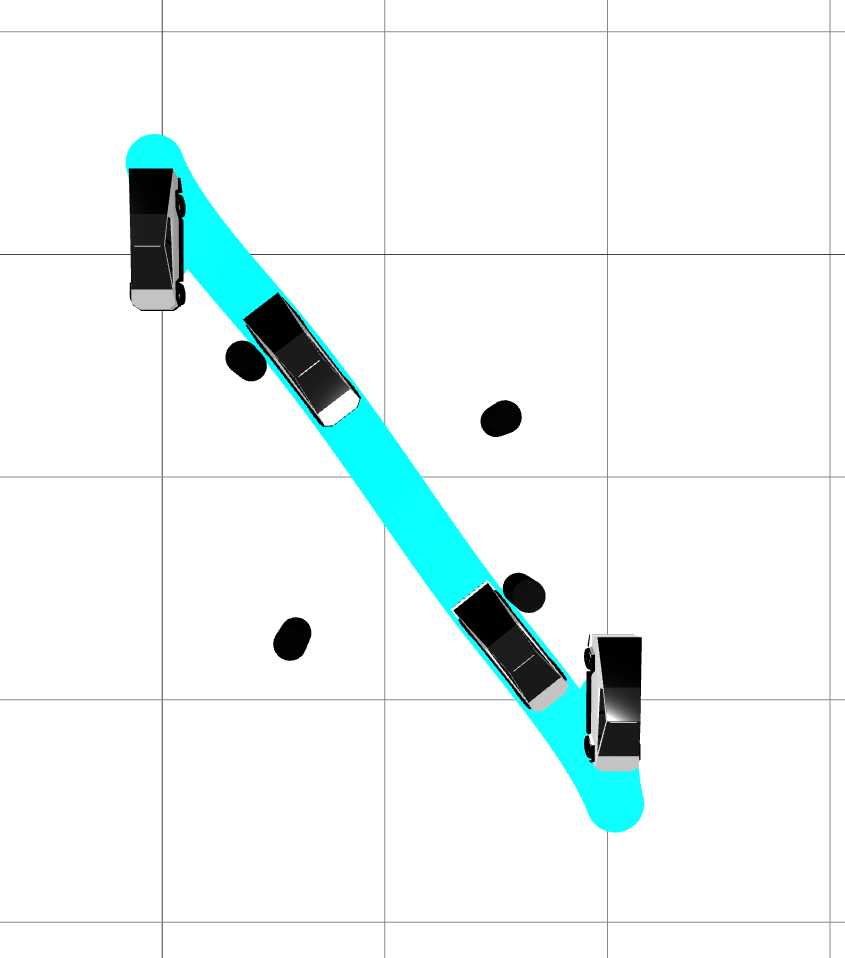
\includegraphics[width=0.32\textwidth]{dpo/car_to.png}
	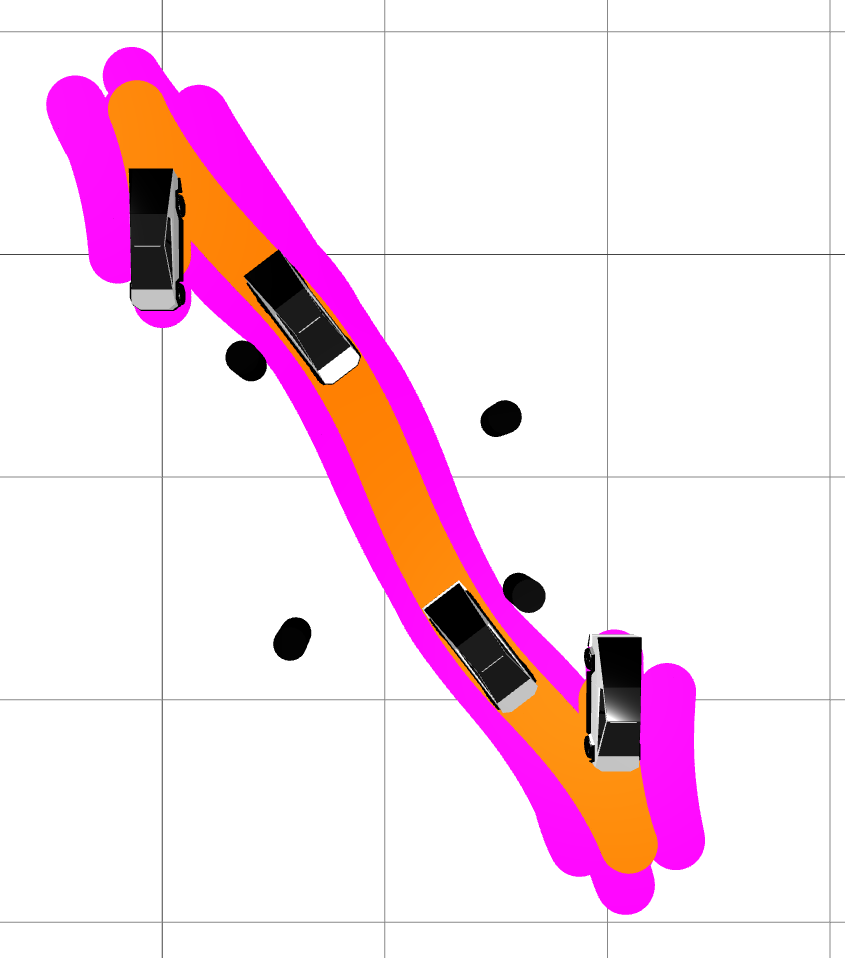
\includegraphics[width=0.32\textwidth]{dpo/car_dpo_sample_1.png}
	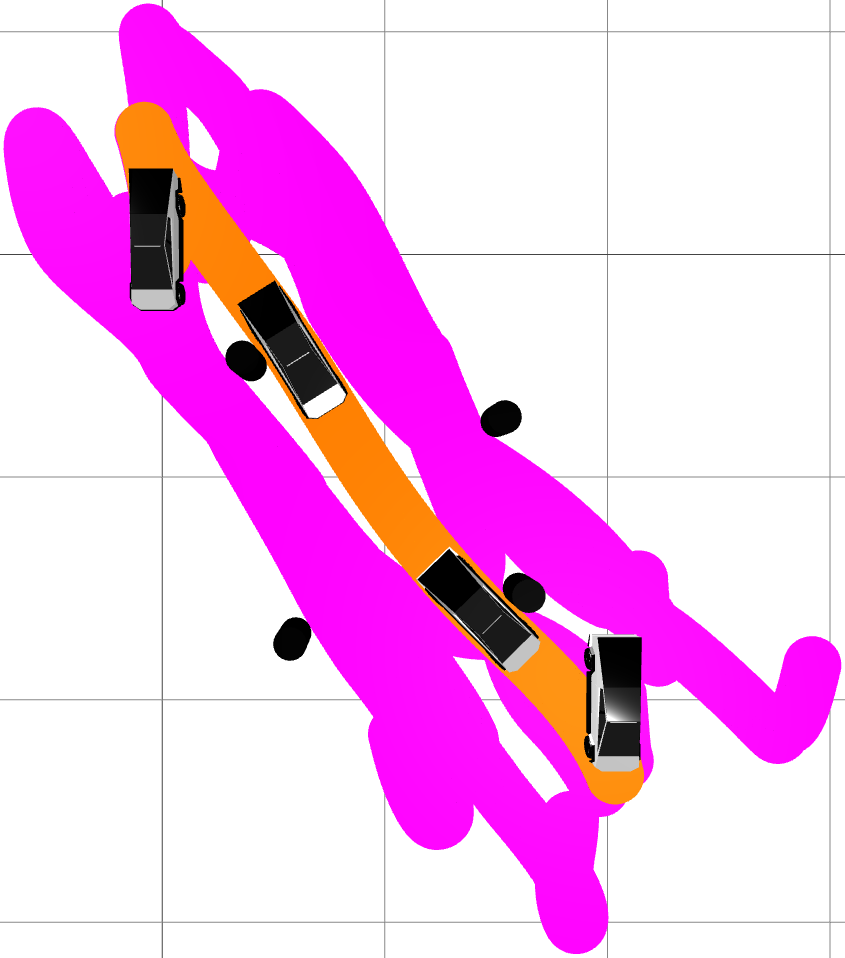
\includegraphics[width=0.32\textwidth]{dpo/car_dpo_sample_2.png}
	\caption[Comparison of car obstacle-avoidance planning with trajectory optimization and Direct Policy Optimization]{Position trajectories for autonomous car avoiding obstacles. TO (left) finds a path that is near the obstacles, whereas DPO with $\delta = 0.001$ (center) finds a path that avoids obstacles with a margin for safety. With larger disturbances, $\delta = 0.01$, samples (magenta) diverge and the DPO policy fails to safely avoid obstacles (right).}
	\label{dpo_car_trajectory}
\end{figure}

\subsection{Cart-pole}
A swing-up trajectory for a cart-pole~\cite{tedrake2014underactuated} with a slider that experiences Coulomb friction is synthesized for horizon $T = 51$ and fixed time step $h = 0.1$. The state, $x = (y, \phi, \dot{y}, \dot{\phi})$, has cart position $y$, pendulum orientation $\phi$, and their respective time derivatives. The optimality conditions for the maximum-dissipation principle~\cite{moreau2011unilateral} are used as constraints to explicitly model friction~\cite{manchester2020variational} with coefficient $\mu_{\text{f}} = 0.1$ for each trajectory. The cart position is controlled and $m = 1$,  there are $d = 4$ disturbance inputs, and the policy has $p = 4$ parameters at each time step. Initial states are sampled from $\mu_1 = 0$ and $P_1 = I$, the weights are $Q_{1:T-1} = \textbf{diag}(10,10,1,1)$, $Q_T = 100I$, and $R_{1:T-1}= I$, and disturbances have $D_{1:T-1} = 0.001 I$.

The performance of LQR tracking reference trajectories optimized subject to friction, as well as the DPO policy, are verified in simulation. Results are provided in Table \ref{dpo_cartpole_results} and tracking for the position and orientation is shown in Fig. \ref{dpo_cartpole_sim}. 

\begin{figure}[H]
	\centering
	\includegraphics{dpo/cartpole_group.tikz}
	\caption[Tracking performance for cart-pole with friction]{Simulated tracking (black) for position (dotted) and orientation (dashed) of cart-pole experiencing Coulomb friction. Comparison between LQR (blue) and DPO (orange) policies.}
	\label{dpo_cartpole_sim}
\end{figure}

By first designing a trajectory that explicitly models friction, it is possible to subsequently synthesize an LQR policy for tracking. In contrast, DPO, which can handle nonsmooth dynamics, produces superior tracking by simultaneously optimizing the reference trajectory and policy.

\begin{table}[H]
	\centering
	\caption[Policy tracking error for cart-pole with friction]{Tracking error, computed with (\ref{dpo_sample_cost}), for cart-pole experiencing Coulomb friction. Comparison between LQR and DPO policies.}
	\begin{tabular}{c c c}
		\toprule
		\textbf{Error} &
		\specialcellbold{LQR} &
		\specialcellbold{DPO} \\
		\toprule
		state & 3.18 & \textbf{2.26}\\
		control & 0.84 & \textbf{0.39}\\
		total & 4.02 & \textbf{2.64}\\
		\toprule
	\end{tabular}
	\label{dpo_cartpole_results}
\end{table}

\subsection{Rocket landing}
We plan a soft landing for a rocket~\cite{meditch1964problem}. The nominal system with planar dynamics has state $x = (y,z,\phi,\dot{y},\dot{z},\dot{\phi})$, with lateral and vertical positions $y$ and $z$, orientation $\phi$, and their respective time derivatives. The rocket is controlled with gimballed thrust, $u = (F_{y},F_{z})$. 

\begin{figure}[H]
	\centering
	\includegraphics[width=0.5\textwidth]{dpo/rocket_schematic.tikz}
	\caption[Planar rocket model]{Rocket with planar dynamics. The model has lateral and vertical positions $y$ and $z$, orientation $\phi$, and thrust inputs $F_y$ and $F_z$. Parameters are inertia $J_{\mathrm{r}}$, mass $m_{\mathrm{r}}$, and length  $l_{\mathrm{r}}$ from center of mass to thruster. A pendulum positioned $d_{\mathrm{f}}$ from rocket center of mass, with orientation $\psi$, length $l_{\mathrm{f}}$, and mass $m_{\mathrm{f}}$, models fuel slosh.}
	\label{dpo_rocket_model}
\end{figure}

It is initialized with non-zero displacements and velocities relative to its target state: a zero-velocity, vertical-orientation touchdown inside a landing zone.

The rocket experiences fuel slosh during landing that is not accounted for in the nominal model. This is a critical dynamical effect, but it is difficult to model and observe. In practice, these unmodeled effects are typically handled in \textit{ad hoc} ways, often with extensive Monte Carlo simulation and controller tuning. To approximately model fuel slosh, we augment the nominal model with two additional states associated with an unobservable and unactuated pendulum (Fig. \ref{dpo_rocket_model}). A common frequency-domain control approach is to include a notch filter at the pendulum's natural frequency in order to prevent excitation of these fuel-slosh dynamics. We instead use DPO to synthesize a policy that is robust to fuel slosh.

The reference trajectory is optimized with the nominal model, while the sample trajectories are subject to the augmented model in order to capture fuel-slosh dynamics, and a linear output feedback policy is optimized that does not have access to the fuel-slosh states. There are $d = 8$ disturbance inputs to the augmented model and the policy has $p = 12$ parameters at each time step. Initial states for the augmented model are sampled with uncertainty $P_1 = I$, weights are $Q_{1:T-1} = 100I$, $Q_T = 1000I$, and $R_{1:T-1} = \textbf{diag}(1,1,100)$, and disturbances have $D_{1:T-1} = 0.001I$. Over the planning horizon $T = 41$ with free final time, thrust limits are enforced.

\begin{figure}[H]
	\centering
	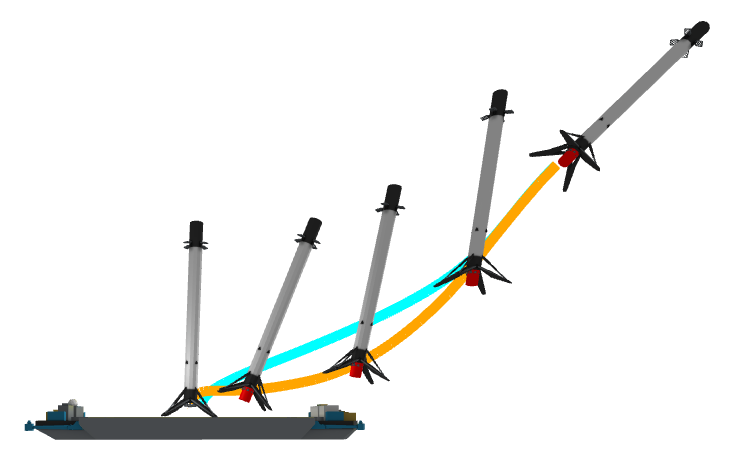
\includegraphics[width=.5\textwidth]{dpo/rocket_landing_ghost.png}
	\caption[Comparison of LQR and Direct Policy Optimization for rocket soft-landing]{Rocket soft-landing position trajectories generated by TO (blue) and DPO (orange). Unlike the TO solution tracked with LQR, the DPO policy successfully lands the rocket despite fuel slosh.}
	\label{dpo_rocket_trajectory}
\end{figure}	

TO finds a 2.72 second solution, whereas DPO finds a longer 2.91 second path to the landing zone. The position trajectories are shown in Fig. \ref{dpo_rocket_trajectory}, simulation results with fuel slosh are provided in Table \ref{dpo_rocket_results}, and tracking results for the rocket's orientation are shown in Fig. \ref{dpo_rocket_tracking}. Due to fuel slosh, LQR fails to track the path generated by TO and the rocket tips over, whereas the DPO policy successfully lands the rocket. 

\begin{figure}[H]
 	\centering
 	\includegraphics{dpo/rocket_orientation_group.tikz}
 	\caption[Orientation tracking performance for rocket soft-landing]{Simulated tracking (black) for the orientation of a rocket experiencing fuel slosh during landing. Comparison between LQR (blue) and DPO (orange) polices.}
 	\label{dpo_rocket_tracking}
\end{figure}

DPO is able to optimize a policy for a system with unobservable dynamical effects by sampling augmented models.

\begin{table}[H]
	\centering
	\caption[Policy tracking error for rocket soft-landing]{Tracking error, computed with (\ref{dpo_sample_cost}), for rocket landing with fuel slosh. Comparison between LQR and DPO policies.}
	\begin{tabular}{c c c}
		\toprule
		\textbf{Error} &
		\specialcellbold{LQR} & 
		\specialcellbold{DPO} \\
		\toprule
		state & 4725.39 & \textbf{5.02}\\
		control & 75.21 & \textbf{0.39}\\
		total & 4800.60 & \textbf{5.41}\\
		\toprule
	\end{tabular}
	\label{dpo_rocket_results}
	\vspace{-0.5cm}
\end{table}

\subsection{Quadrotor}
A point-to-point maneuver is planned for a quadrotor~\cite{mellinger2012trajectory} that experiences a random blade breaking off from a propeller during flight. 

A broken propeller is modeled by constraining the corresponding control input to be half its nominal maximum value. We use DPO to optimize a policy that is robust to this event occurring for any of the propellers. The reference model has no broken propellers, but the sample trajectories are optimized with different models from four groups, each experiencing a different broken propeller. There are $n = 12$ states, $m = 4$ controls, $d = 12$ input disturbances, and the policy has $p = 48$ parameters at each time step. Initial states are sampled around the initial nominal state with uncertainty $P_1 = I$, weights are $Q_{1:T-1} = 10I$, $Q_T = 100I$, and $R_{1:T-1} = I$, and disturbances have $D_{1:T-1} = 0.001 I$. Thrust limits are enforced over the planning horizon $T=31$ with a free final time.	

TO finds a 2.71 second trajectory, while DPO finds a longer 3.38 second trajectory with lower maximum controls (Fig. \ref{dpo_quadrotor_control}). 

\begin{figure}[H]
	\centering
	\includegraphics{dpo/quadrotor_control_group.tikz}
	\caption[Action trajectory comparison between trajectory optimization and Direct Policy Optimization for quadrotor]{Nominal controls for quadrotor performing point-to-point maneuver generated with TO (blue) and DPO (orange). The controls found with DPO are applied over a longer horizon and have lower maximum values compared to TO.}
	\label{dpo_quadrotor_control}
\end{figure}

The policies are compared in simulation over 100 initial conditions with noise sampled from $\mathcal{N}(0, 0.001 I)$. One set of initial conditions is visualized in Fig. \ref{dpo_quadrotor_prop}. 

\begin{figure}[H]
	\centering
	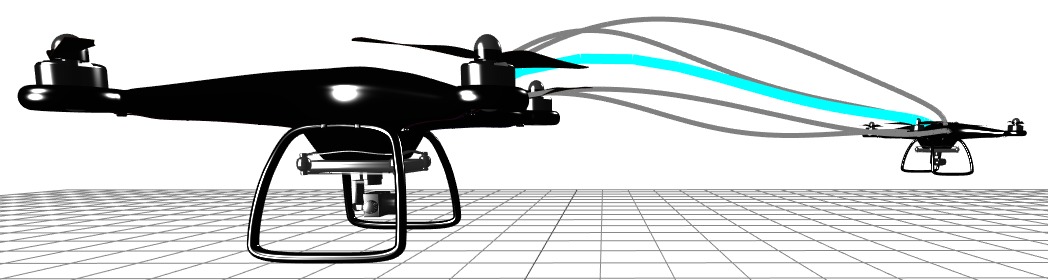
\includegraphics[width=.45\textwidth]{dpo/quadrotor_to_grid.png}
	\vspace{0.01\textwidth}
	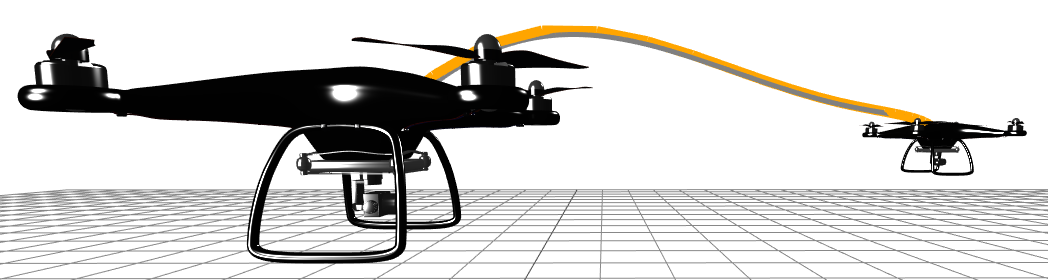
\includegraphics[width=.45\textwidth]{dpo/quadrotor_dpo_grid.png}
	\caption[Tracking comparison for LQR and Direct Policy Optimization for quadrotor]{Simulated position trajectories (gray) for quadrotor controlled with LQR (top) and DPO (bottom) policies while experiencing different propellers breaking. LQR (blue) has degrading tracking while DPO (orange) has superior, and nearly identical tracking regardless of which propeller breaks.}
	\label{dpo_quadrotor_prop}
\end{figure}

The average tracking performance over each propeller breaking is provided in Table \ref{dpo_quad_prop_results}. DPO finds a policy with consistent and superior tracking compared with LQR for all cases by optimizing over different models.

\begin{table}[H]
	\centering
	\caption[Policy tracking error for quadrotor]{Tracking errors with mean ($\mu$) and standard deviation ($\sigma$), computed with (\ref{dpo_sample_cost}), comparing LQR and DPO policies for quadrotor over 100 initial conditions for each propeller being broken.}
	\begin{subtable}[t]{0.85\textwidth}
		\centering
		\begin{tabular}{c c c}
			\toprule
			\textbf{Error ($\mu$, $\sigma$)} &
			\specialcellbold{LQR} & 
			\specialcellbold{DPO} \\
			\toprule
			state & (13.43, 12.64) & \textbf{(4.74, 5.87)} \\
			control & (0.074, 0.067) & \textbf{(0.020, 0.022)} \\
			total & (13.50, 12.71) & \textbf{(4.76, 5.89)}\\
			\toprule
		\end{tabular}
		\caption{propeller 1 broken}
		\vspace{1em}
	\end{subtable}
	\vfill
	\begin{subtable}[t]{0.85\textwidth}
		\centering
		\begin{tabular}{c c c}
			\toprule
			\textbf{Error ($\mu$, $\sigma$)} &
			\specialcellbold{LQR} & 
			\specialcellbold{DPO} \\
			\toprule
			state & (13.13, 11.98) & \textbf{(4.74, 5.87)} \\
			control & (0.073, 0.065) & \textbf{(0.020, 0.023)} \\
			total & (13.21, 12.05) & \textbf{(4.76, 5.89)}\\
			\toprule
		\end{tabular}
		\caption{propeller 2 broken}
		\vspace{1em}
	\end{subtable}
	\vfill
	\begin{subtable}[t]{0.85\textwidth}
		\centering
		\begin{tabular}{c c c}
			\toprule
			\textbf{Error ($\mu$, $\sigma$)} &
			\specialcellbold{LQR} & 
			\specialcellbold{DPO} \\
			\toprule
			state & (3431.91, 12895.93) & \textbf{(4.74, 5.88)} \\
			control & (2.21, 7.86) & \textbf{(0.020, 0.023)} \\
			total & (3434.12, 12903.75) & \textbf{(4.76, 5.90)}\\
			\toprule
		\end{tabular}
		\caption{propeller 3 broken}
		\vspace{1em}
	\end{subtable}
	\vfill
	\begin{subtable}[t]{0.85\textwidth}
		\centering
		\begin{tabular}{c c c}
			\toprule
			\textbf{Error ($\mu$, $\sigma$)} &
			\specialcellbold{LQR} & 
			\specialcellbold{DPO} \\
			\toprule
			state & (4843.89, 14892.19) & \textbf{(4.74, 5.87)} \\
			control & (3.21, 9.41) & \textbf{(0.020, 0.023)} \\
			total & (4847.10, 14901.59) & \textbf{(4.76, 5.89)}\\
			\toprule
		\end{tabular}
		\caption{propeller 4 broken}
	\end{subtable}
	\label{dpo_quad_prop_results}
\end{table}

\section{Limitations} \label{dpo_limitations}
We empirically demonstrate through Monte Carlo simulations that DPO recovers LQR policies for a double integrator system. It seems possible that for LQG problems, despite the non-convexity of the policy constraints, there exists a unique global solution for DPO. However, we leave a formal convergence analysis to future work.

The motion-planning examples highlight a number of DPO's capabilities compared to DIRTREL and GPS. In the cart-pole example, DPO is able to subject each trajectory to discontinuous Coulomb friction calculated with the maximum-dissipation principle, whereas a similar DIRTREL example only applied white-noise disturbances to a single model~\cite{manchester2019robust}. This example also highlights how jointly optimizing trajectories and a policy leads to superior performance, a distinction compared to the decoupled approach employed by GPS. Next, in the rocket landing example, DPO optimizes an output feedback policy, whereas DIRTREL is limited to state feedback. Additionally, directly modeling fuel-slosh dynamics with a pendulum is likely simpler than designing input disturbances for DIRTREL to capture the same effects. Finally, with DPO, additional constraints can be applied to any of the decision variables, whereas the ability of GPS to handle constraints using DDP and stochastic gradient descent is limited.

Because we use local optimization methods to solve DPO, providing good initial guesses to the solver is crucial for performance of the algorithm. In practice, we use a standard TO solution to warm start the reference and sample trajectories for DPO. For linear state-feedback policies, we use the corresponding LQR solution as an initial guess. While not necessary in any of our examples, initial guesses for more complex policies could be found by running DPO without the policy constraint, then performing an offline regression to fit approximate policy parameters for warm starting. 

For a TO problem solved with a sparsity-exploiting second-order method, the computational complexity is approximately $O\Big( T (n + m)^3 \Big)$~\cite{wang2009fast}. For DPO, we can consider an augmented state and control with dimensions $n(2n + 2)$ and $m(2n + 2)$, respectively. The complexity of DPO is, therefore, $O\Big( T (n^6 + m^3n^3) \Big)$. In the examples, which do not employ a specialized solver, solution times range from seconds to 1.5 hours for a state with $n = 12$ on a laptop computer. It is likely possible to exploit the DPO problem's structure to improve the complexity by using custom linear solvers. First-order methods, which can scale much better, become attractive for DPO as problems become large.

Lastly, LQR is a powerful tool and can likely be tuned to qualitatively match the performance of the linear policies found with DPO in many cases. However, the strength of DPO lies in its ability to explicitly reason about robustness and the complex coupling between dynamics, constraints, and disturbances during synthesis, instead of relying on hand tuning and heuristics.

\section{Future work}\label{dpo_future_work}

We have presented a new algorithm, Direct Policy Optimization, for approximately solving stochastic optimal-control problems. We demonstrate that the algorithm is exact in the LQG case and is capable of optimizing policies for nonlinear systems that respect control limits and obstacles, and are robust to unmodeled dynamics.

Many interesting avenues for future work remain: Extensions to nonlinear policies could be made by introducing high-dimensional features and regularization or constraints on policy parameters, or neural networks could be used to parameterize policies since the policy parameters scale much better compared to state and control dimensions. Another potential direction is to optimize a local value function approximation in place of an explicit policy. A much richer class of disturbances and model parameter uncertainty could also be modeled by augmenting the state vector and dynamics. Lastly, more complex systems with larger state and input dimensions may be more amenable to optimization with first-order or matrix-free methods.


\chapter{Contact-Implicit Predictive Control}

We present a general approach for controlling robotic systems that make and break contact with their environments. Contact-implicit model predictive control (CI-MPC) generalizes linear MPC to contact-rich settings by utilizing a bi-level planning formulation with lower-level contact dynamics formulated as time-varying linear complementarity problems (LCPs) computed using strategic Taylor approximations about a reference trajectory. These dynamics enable the upper-level planning problem to reason about contact timing and forces, and generate entirely new contact-mode sequences online. To achieve reliable and fast numerical convergence, we devise a structure-exploiting interior-point solver for these LCP contact dynamics and a custom trajectory optimizer for the tracking problem. We demonstrate real-time solution rates for CI-MPC and the ability to generate and track non-periodic behaviours in hardware experiments on a quadrupedal robot. We also show that the controller is robust to model mismatch and can respond to disturbances by discovering and exploiting new contact modes across a variety of robotic systems in simulation, including a pushbot, planar hopper, planar quadruped, and planar biped.

\vspace*{\fill}

\noindent Fast Contact-Implicit Model Predictive  Control. Simon Le Cleac'h$^*$, Taylor A. Howell$^*$, Shuo Yang, Chi-Yen Lee, John Zhang, Arun Bishop, Mac Schwager, and Zachary Manchester. arXiv 2107.05616. 2022.

\pagebreak 

\section{Introduction} \label{cipc_introduction}
Controlling systems that make and break contact with their environments is one of the grand challenges in robotics. Numerous approaches have been employed for controlling such systems, ranging from hybrid-zero dynamics \cite{westervelt2003hybrid, ames2014rapidly, li2021reinforcement}, to complementarity controllers \cite{aydinoglu2020contact}, to neural-network policies \cite{heess2017emergence,heiden2020neuralsim}, and model predictive control (MPC) \cite{winkler2018gait, sleiman2021unified}. There have also been numerous successes deploying such approaches on complex systems in recent years: direct trajectory optimization and LQR on Atlas \cite{kuindersma2016optimization}, smooth-contact models and differential dynamic programming on HRP-2  \cite{todorov2012mujoco, tassa2012synthesis, koenemann2015whole}, zero-moment point and feedback linearization on ASIMO \cite{hirai1998development}, and MPC with simplified dynamics models on Cheetah \cite{bledt2020regularized} and ANYmal \cite{lee2020learning}. However, reliable \emph{general-purpose} control techniques that can reason about contact events and can be applied across a wide range of robotic systems without requiring application-specific model simplifications, gait-generation heuristics, or extensive parameter tuning remain elusive.

Our approach combines fast, differentiable rigid-body dynamics with contact, strategic approximations about a reference trajectory, and specialized numerical optimization techniques for the application of local tracking control for systems that experience contact interactions with their environments. The result is a bi-level model predictive control algorithm that can effectively reason about contact changes in the presence of large disturbances while remaining fast enough for real-time execution.

We formulate contact dynamics as a complementarity problem and devise a fast interior-point solver to reliably optimize this feasibility problem. Smooth gradients are efficiently computed through the non-smooth dynamics by exploiting intermediate solutions from within this solver using implicit differentiation. To enable real-time performance for control, we pre-compute linearizations of the system's dynamics, signed-distance functions, and friction cones about a reference trajectory, while explicitly retaining complementarity constraints that encode contact switching behavior, resulting in a sequence of lower-level time-varying linear-complementarity problems (LCP) which represent the model's contact dynamics. An upper-level trajectory optimization problem is then optimized using fast linear algebra. We refer to this algorithm as \textit{Contact-Implicit Model Predictive Control} (CI-MPC).

Finally, we demonstrate that CI-MPC can generate new contact sequences online and reliably track reference trajectories despite significant model mismatch and while large external disturbances are applied for a number of qualitatively different robotic systems, including: a pushbot, and planar hopper, quadruped, and biped systems in simulation; and on Unitree Go1 quadruped hardware \cite{unitree_go1}.

Our contributions are:
\begin{itemize}
	\item Fast approximate contact dynamics that can be reliably evaluated and efficiently differentiated with a custom interior-point solver
	\item Structure-exploiting solvers for the contact-dynamics and trajectory optimization problems
	\item A model predictive control framework for robotic systems with contact dynamics
	\item A collection of simulation and hardware experiments demonstrating the performance of CI-MPC on a variety of robotic systems across a range of highly dynamic tasks
\end{itemize}

In the remainder of this paper, we first review related work on control through contact with MPC, as well as complementarity-based contact dynamics in Section \ref{cipc_related_work}. Next, we present a brief overview of MPC, outline the classic complementarity formulation for contact dynamics, and provide background on interior-point methods and implicit differentiation in Section \ref{cipc_background}. Then, we present CI-MPC in Section \ref{cimpc}. Results are presented in Section \ref{cipc_results} including both simulation and hardware experiments. Finally, we discuss our results, limitations of this approach in Section \ref{cipc_limitations} and potential directions for future work in Section \ref{cipc_future_work}.

\section{Related Work} \label{cipc_related_work}
In this section, we review related work on MPC for the control of dynamical systems that make and break contact with their environments and provide an overview of complementarity-based contact dynamics.

\subsection{Model Predictive Control}

Today, most successful approaches for controlling legged robots utilize MPC in combination with simplified models and heuristics originally pioneered by Raibert for hopping robots \cite{raibert1989dynamically}. The key insight of this work is that the control problem can be decoupled into a high-level controller that plans body motions while ignoring the details of the leg dynamics, and a low-level controller that determines the necessary leg motions and joint torques to generate the forces and torques on the body determined by the high-level controller.

Arguably the most impressive control work on humanoids has utilized centroidal dynamics with full kinematics to enable Atlas to navigate various scenarios with obstacles \cite{dai2014whole} and perform parkour \cite{atlas2019parkour}. Integrating hardware design and controller synthesis has also recently enabled small humanoids to perform agile acrobatic maneuvers in simulation \cite{chignoli2021humanoid}.

There have also been impressive advances for quadrupeds, achieved by designing hardware that aims to closely match the modeling approximations made in the controller, e.g., building very light legs \cite{bledt2020regularized}. Whole-body control, which has the benefit of simpler overall control structures and the ability to leverage a system's dynamics, has been achieved at real-time rates on hardware \cite{neunert2018whole}. Approaches that utilize both force-based MPC and whole-body control have also demonstrated agile locomotion \cite{kim2019highly}.

A major limitation of these prior works is that the control policies are highly specialized to a specific robotic system. In this work, we compare CI-MPC to a number of system-specific control methods that perform quite well for their given system, but do not generalize to other systems, whereas our policy generalizes to many different systems that experience contact interactions while achieving comparable or better performance.

\subsection{Complementarity-Based Contact Dynamics}
The classic approach for simulating rigid-body dynamics with contact interactions is a velocity-based time-stepping scheme formulated as a linear complementarity problem (LCP). The LCP searches for the next state of the system while enforcing impact and friction constraints. Solvers for this class of problems utilize pivoting methods 
\cite{drumwright2015rapidly}, such as Lemke's algorithm \cite{cottle2009linear}, or interior-point methods \cite{kojima1991unified}. Implementations of pivoting methods can be found in general-purpose LCP solvers such as PATH \cite{dirkse1995path}, or physics engines including: Bullet \cite{coumans2019} and DART \cite{lee2018dart}. 

Derivatives of LCP-based contact dynamics can be efficiently computing using implicit differentiation \cite{dini1907lezioni}. However, the quality of these results is dependent on the method employed for optimization. Pivoting approaches enforce strict complementarity at each iteration, returning solutions at non-differentiable points. As a consequence, this differentiation will return subgradients that make, typically efficient, second-order optimization slower and less reliable. In contrast, interior-point methods relax the complementarity constraints at each iteration, only converging in the limit. These intermediate results can be implicitly differentiated to return smooth gradients \cite{howell2022dojo}. Alternative approaches for computing gradients for contact dynamics include utilizing auto-differentiation tools \cite{heiden2020neuralsim} and analyzing the LCP solution to select subgradients \cite{werling2021fast}.

In addition to simulation, contact dynamics represented as LCPs have been utilized for planning. Collocation approaches \cite{stryk1993numerical} directly encode the LCP problem as  as constraints in order to enforce contact dynamics, along with an objective specifying desired behavior, in a large non-convex problem \cite{posa2014direct}. This approach enables the optimizer to plan without pre-specified mode sequences for locomotion and simple manipulation tasks. Subsequent work improved this approach by introducing higher-order integrators for the dynamics and a numerically robust, exact $\ell_1$-penalty for handling the complementarity constraints \cite{manchester2020variational}. Alternative rollout-based approaches utilize LCPs for forward simulation and subsequently differentiate through the solution of one-step dynamics in order to compute derivatives for gradient-based optimization \cite{de2018end,werling2021fast}.

Another popular contact-dynamics formulation is MuJoCo's soft-contact model \cite{todorov2012mujoco}, which solves a convex optimization problem and trades physical realism for fast and reliable performance. An alternative model solved a strictly convex quadratic program \cite{anitescu2006optimization}. Gradients are computed use a finite-difference scheme. However, this approach is computationally less efficient. Additionally, the LCP complementarity constraints can be relaxed, resulting in a soft-contact model that exhibits improved numerical properties in some scenarios \cite{geilinger2020add}. 

\section{Background} \label{cipc_background}
In this section, we provide technical background on MPC, complementarity-based contact dynamics, interior-point methods, and implicit differentiation.

\subsection{Model Predictive Control}
Predictive control policies \cite{richalet1978model} optimize a planning problem:
\begin{equation}
	\begin{array}{ll}
		\underset{x_{1:T}, u_{1:T-1}}{\mbox{minimize}} & g_T(x_T) + \sum \limits_{t = 1}^{T-1} g_t(x_t, u_t) \label{cipc_trajectory_optimization}\\
		\mbox{subject to} & x_{t+1} = f_t(x_t,u_t), \quad t = 1,\dots,T-1,\\
		& (x_1~\mbox{given}),
	\end{array}
\end{equation}
for a given initial state in order to compute controls for a dynamical system we aim to control. If planning is performed at a sufficiently high rate, the sequence of open-loop plans provide \textit{feedback}. For a system with state $x \in \mathbf{R}^{n}$, control $u \in \mathbf{R}^{m}$, time index $t$, initial state $x_1$, and discrete-time dynamics $f : \mathbf{R}^{n} \times \mathbf{R}^{m} \rightarrow \mathbf{R}^{n}$, the optimizer aims to minimize an objective with costs, $g: \mathbf{R}^{n} \times \mathbf{R}^{m} \rightarrow \mathbf{R}$, over a planning horizon $T$.

Solving a (potentially) non-convex problem \eqref{cipc_trajectory_optimization} online can be unreliable or computation too expensive. Instead, a proxy problem is solved online that makes strategic approximations. A common simplification is to track a reference trajectory, $\bar{\tau} = (\bar{x}_1, \bar{u}_1, \dots, \bar{x}_T$), denoted with an overbar ($\bar{\phantom{a}}$), that is precomputed offline. In this setting, the computational complexity for planning is reduced by utilizing dynamics:
\begin{equation}
	\delta x_{t+1} = A_t \delta x_t + B_t \delta u_t, \label{cipc_linear_dynamics}
\end{equation}
linearized about the reference, where $A = \partial f(\bar{x}, \bar{u}) / \partial x$, $B = \partial f(\bar{x}, \bar{u}) / \partial x$, and the decision variables are relative to the reference trajectory, i.e., $\delta a = a - \bar{a}$; and a quadratic objective:
\begin{equation}
	\frac{1}{2}\delta x_t^T Q_t \delta x_t + q_t^T \delta x_t + \frac{1}{2}\delta u_t^T R_t \delta u_t  + r_t^T \delta u_t, \label{cipc_quadratic_objective}
\end{equation}
where $Q = \partial^2 g(\bar{x}, \bar{u}) / \partial x^2, q = \partial g(\bar{x}, \bar{u}) / \partial x, R = \partial^2 g(\bar{x}, \bar{u}) / \partial u^2, r = \partial g(\bar{x}, \bar{u}) / \partial u$, similarly comprise a second-order expansion about the reference trajectory.

This formulation, potentially with additional affine state and control constraints, is commonly referred to as \textit{linear} MPC. Without such constraints, the problem 
(\ref{cipc_trajectory_optimization}) with linear dynamics \eqref{cipc_linear_dynamics} and quadratic objective \eqref{cipc_quadratic_objective} is the LQR problem \cite{kalman1964lqr} and is efficiently solved with a backward Riccati recursion. 

Predictive control iteratively optimizes \eqref{cipc_trajectory_optimization}, or an approximate version of it (\ref{cipc_linear_dynamics} - \ref{cipc_quadratic_objective}), for a given state, and the optimized controls are utilized to compute an input for the system. After the system evolves, the problem is re-optimized for a new state in order to compute a new control for the system. By repeating this procedure at a high rate, feedback control is achieved \cite{wang2009fast}. In practice, applying the controls optimized with time-varying linearized dynamics and quadratic costs, to the actual nonlinear system is extremely effective, especially for applications that track a reference trajectory.
{\small }
\subsection{Complementarity-Based Contact Dynamics}

Contact dynamics can be simulated with a velocity time-stepping scheme \cite{stewart1996implicit}, formulated as complementarity problem \cite{cottle2009linear}: 
\begin{align}
	\label{cipc_feas_prob}
	{\mbox{find}} \quad & q, \lambda,\eta, \beta, \psi \\
	\mbox{subject to} \quad & \left[M_{+}(q - q_{-}) - M_{-}(q_{-} - q_{--})\right] / h + h C =  J^T \lambda + B u, \label{cipc_smooth_dynamics}\\
	& \gamma \circ \phi = 0, \label{cipc_impact_complementarity}\\
	& \beta \circ \left[ P (q - q_{-})/h + \psi \textbf{1} \right] = 0, \label{cipc_friction_complementarity} \\
	& \psi \circ \left[\mu \gamma - \textbf{1}^T \beta \right] = 0, \label{cipc_friction_velocity_complementarity}\\
	& \phi, \gamma \geq 0, \label{cipc_impact_inequalities} \\
	& \beta, \psi, [P (q - q_{-})/h + \psi \textbf{1}], [\mu \gamma - \textbf{1}^T \beta] \geq 0, \label{cipc_friction_inequalities}
\end{align}
that finds the next configuration of the system $q \in \mathbf{R}^{n_q}$ using implicitly defined velocities, $v = (q - q_{-}) / h \in \mathbf{R}^{n_v}$. Subscripts indicate a previous time step. This formulation considers a single contact point, but generalizes to systems with multiple contacts.
The problem utilizes: the mass matrix $M: \mathbf{R}^{n_q} \rightarrow \mathbf{S}_{++}^{n_v}$; dynamics bias $C: \mathbf{R}^{n_q} \times \mathbf{R}^{n_v} \rightarrow \mathbf{R}^{n_v}$ that includes Coriolis and gravitational terms; contact Jacobian $J: \mathbf{R}^{n_q} \rightarrow \mathbf{R}^{d \times n_v}$ that maps contact forces in the contact frame into the generalized coordinates; input Jacobian $B: \mathbf{R}^{n_q} \rightarrow \mathbf{R}^{n_v \times m}$ that maps control inputs, typically joint torques, into the generalized coordinates; $P: \mathbf{R}^{n_q} \rightarrow \mathbf{R}^{p (d-1) \times n_v}$ is a mapping from the generalized velocity space to an overparameterized contact tangent space; time step $h \in \mathbf{R}_{+}$; contact forces $\lambda = (\gamma, \beta) \in \mathbf{R}^d$ defined in the contact frame, with normal force $\gamma \in \mathbf{R}$ and overparameterized friction forces $\beta \in \mathbf{R}^{p (d - 1)}$ that are constrained by a linearized friction cone; $\psi \in \mathbf{R}$ is a dual variable associated with friction, representing the magnitude of the contact point velocity; signed-distance function, $\phi: \mathbf{R}^{n_q} \rightarrow \mathbf{R}$, that returns distance between a specified contact point on the robot (e.g., feet) and the closest surface in the environment (e.g., the floor); and where $\circ$ is an element-wise (Hadamard) vector product. We use $p$ to denote the overparameterization dimension (often $p$ = 2) and $d$ to denote the environment dimension $d = 2$ for planar systems and $d = 3$ otherwise.

The smooth dynamics \eqref{cipc_smooth_dynamics} are discretized with a semi-implicit Euler scheme \cite{marsden2001discrete}; complementarity constraints (\ref{cipc_impact_complementarity}- \ref{cipc_friction_velocity_complementarity}) encode contact switching behavior; impact is encoded in \eqref{cipc_impact_complementarity} and \eqref{cipc_impact_inequalities}; and friction terms (\ref{cipc_friction_complementarity}-\ref{cipc_friction_velocity_complementarity}) and \eqref{cipc_friction_inequalities}, are derived from the maximum dissipation principle \cite{moreau2011unilateral}.

Problem data include previous configurations $q_{-}, q_{--}$, time step $h$ and control inputs $u$. A nonlinear formulation uses the following mappings:
\begin{align}
	&M_{+} \leftarrow M(q), 
	&&M_{-} \leftarrow M(q_{-}), \notag \\ 
	&C \leftarrow C(q, (q - q_{-}) / h), 
	&&J \leftarrow J(q),  \\ 
	&B \leftarrow B(q), 
	&& P \leftarrow P(q), \notag \\ 
	& \phi \leftarrow \phi(q), \notag
\end{align}
evaluating these terms at the next configuration. In practice, a partial linearization of the dynamics is performed to satisfy a linear complementarity problem (LCP) \cite{stewart1996implicit}, resulting in the following mappings:
\begin{align}
	&M_{+} \leftarrow M(q_{-}), 
	&&M_{-} \leftarrow M(q_{--}), \notag \\ 
	&C \leftarrow C(q_{-}, (q_{-} - q_{--}) / h), 
	&&J \leftarrow J(q_{-}),  \\ 
	&B \leftarrow B(q_{-}), 
	&& P \leftarrow P(q_{-}), \notag \\
	& \phi \leftarrow \phi(q_{-}) + N(q{-}) (q - q_{-}), \notag
\end{align}
where $N = d \phi / d q$.

\subsection{Interior-Point Method}
Classically, LCPs are solved using active-set methods \cite{dirkse1995path}, which strictly enforce complementarity at each iteration. An alternative approach is interior-point methods \cite{kojima1991unified, nocedal2006numerical}, which relax these conditions during intermediate iterations, only satisfying these constraints in the limit.

LCPs can be generally formulated as:
\begin{equation}
	\begin{array}{ll}
		\mbox{find}       & x, y, z \\
		\mbox{subject to} & E x + F y + f = 0,\\
		& G x + H y + z + h = 0,\\
		& y \circ z = 0,\\
		& y, z \geq 0,\\
	\end{array} \label{cipc_lcp_problem}
\end{equation}
with decision variables $x \in \mathbf{R}^n$, $y, z \in \mathbf{R}^m$ and problem data $\theta = (E, F, G, H, f, h)  \in \mathbf{R}^{n \times n} \times \mathbf{R}^{n \times m} \times \mathbf{R}^{m \times n} \times \mathbf{R}^{m \times m} \times \mathbf{R}^n \times \mathbf{R}^m = \mathbf{R}^p$. Interior-point methods parameterize (\ref{cipc_lcp_problem}) by a  central-path parameter $\kappa \in \mathbf{R}_{+}$ that relaxes the following bilinear constraint:
\begin{equation}
	y \circ z = \kappa \textbf{1},
\end{equation}
where $\textbf{1}$ a vector of ones. 

The equality and relaxed bilinear constraints form a residual vector or solution map, $r: \mathbf{R}^{n + 2m} \times \mathbf{R}^p  \times \mathbf{R}_{+} \rightarrow \mathbf{R}^{n + 2m}$, that takes $w = (x, y, z) \in \mathbf{R}^{n + 2m}$, the problem data, and central-path parameter as inputs. The problem data and central-path parameter are fixed during optimization. In the context of contact dynamics, these data encode the mechanical properties of the robots, its current configuration and velocity, and properties of the environment like friction coefficients.
Newton or quasi-Newton methods are used to find search directions that reduce the norm of the residual and a backtracking line search is employed to ensure that the inequality constraints are strictly satisfied for candidate points at each iteration. Once the residual is optimized to a desired tolerance, the central-path parameter is decreased and the new subproblem is warm-started with the current solution and then optimized. This procedure is repeated in order to find solutions to (\ref{cipc_lcp_problem}) with $\kappa \rightarrow 0$ until the central-path parameter, also referred to as complementary slackness, is below a desired tolerance.

Importantly, our interior-point method utilizes a predictor-corrector algorithm \cite{mehrotra1992implementation} that leads to significantly improved convergence. First, the corrector step modifies the pure Newton search direction and typically reduces the number of iterations required for convergence by half (compared to the pure search direction). Second, the central-path parameter is adapted at each iteration to prevent premature numerical ill-conditioning. In practice, we find that this approach is significantly more reliable and has improved convergence behavior compared to prior work that employed relaxed complementarity conditions \cite{manchester2020variational}.

In addition to simulating contact by solving a feasibility problem, we would like to compute gradients of these dynamics, requiring us to differentiate through an optimization problem. This is accomplished with implicit differentiation \cite{dini1907lezioni}.

For the interior-point method \eqref{cipc_lcp_problem}, the residual is:
\begin{equation}
	r(w; \theta) = \begin{bmatrix} E x + F y + f \\ G x + H y + z + h \\ y \circ z - \kappa \textbf{1}\end{bmatrix}.
\end{equation}
A differentiable interior-point method is summarized in Algorithm \ref{cipc_ip_algo}. Importantly, we can compute gradients for intermediate results, corresponding to non-zero values for the central-path parameter, i.e., $\kappa_{\mbox{grad}} \neq 0$. For additional details about differentiating through intermediate results of contact dynamics that are solved with interior-point methods, see \cite{howell2022dojo}.

\begin{algorithm}[H]
	\caption{Differentiable Interior-Point Method}\label{cipc_ip_algo}
	\begin{algorithmic}[1]
		\Procedure{Optimize}{$x, \theta$}
		\State \textbf{Settings}: $\beta = 0.5, \gamma = 0.1, \epsilon_{\kappa} = 10^{-6}, \epsilon_{r} = 10^{-8}$
		\State \textbf{Initialize}: $y, z = \mathbf{1}, \kappa = 0.1, \kappa_{\mbox{grad}} = 10^{-4}$
		\State \textbf{Until} $\kappa < \epsilon_{\kappa}$ \textbf{do} 
		\State \indent $\Delta w = (\frac{\partial r}{\partial w})^{-1} r(w; \theta, \kappa)$
		\State \indent $\alpha \leftarrow 1$
		\State \indent \textbf{Until} $(y, z) - \alpha (\Delta y, \Delta z) > 0$ \textbf{do} $\alpha \leftarrow \beta \alpha$
		\State \indent \textbf{Until} $\|r(w-\alpha\Delta w; \theta, \kappa)\| < \|r(w; \theta, \kappa)\|$ \textbf{do}
		\State \indent \indent $\alpha \leftarrow \beta \alpha$
		\State \indent $w \leftarrow w - \alpha \Delta w$
		\State \indent \textbf{If} $\|r(w; \theta, \kappa)\| < \epsilon_{r}$ \textbf{do} $\kappa \leftarrow \gamma \kappa$
		\State $\frac{\partial w}{\partial \theta} \leftarrow \textbf{Differentiate}(w, \theta, \kappa_{\mbox{grad}})$ \Comment{Eq. \ref{intro_solution_sensitivity}}
		\State \textbf{Return} $w, \frac{\partial w}{\partial \theta}$ 
		\EndProcedure
	\end{algorithmic}
\end{algorithm}

\section{Contact-Implicit Model Predictive Control} \label{cimpc}
In this section we present Contact-Implicit Model Predictive Control, a tracking policy for systems that make and break contact with their environments. First, we formulate time-varying LCP contact dynamics that are selectively approximated about a reference trajectory. Then, we devise a fast solver for the resulting LCP. Next, we discuss how to compute smooth gradients through the dynamics. A bi-level planning formulation, which utilizes these dynamics for direct trajectory optimization \cite{von1992direct}, follows. To enable the policy to work well in environments with uncertain terrain we propose a contact-height heuristic. Finally, we summarize the approach and provide an algorithm for CI-MPC.

\subsection{Time-Varying Contact Dynamics}
We formulate alternative LCP dynamics that utilize a reference trajectory, resulting in the following mappings: 
\begin{align}
	&M_{+} \leftarrow M(\bar{q}), 
	&&M_{-} \leftarrow M(\bar{q}_{-}), \notag \\ 
	&C \leftarrow C(\bar{q}, (\bar{q} - \bar{q}_{-}) / h), 
	&&J \leftarrow J(\bar{q}),  \\ 
	&B \leftarrow B(\bar{q}), 
	&& P \leftarrow P(\bar{q}), \notag \\
	& \phi \leftarrow \phi(\bar{q}) + N(\bar{q}) (q - \bar{q}). \notag
\end{align}
The LCP problem, formulated for an interior-point method, has the form:
\begin{align}
	\begin{array}{ll}
		{\mbox{find}} & w \\
		\mbox{subject to} 
		& C (w - \bar{w}) + D (\theta - \bar{\theta}) = 0 \\
		& \gamma \circ s_{\phi}  = \kappa \textbf{1}, \\
		& \psi \circ s_{\psi} = \kappa \textbf{1}, \\
		& \beta \circ \eta = \kappa \textbf{1}, \\
		& \gamma, \psi, \beta, \eta, s_{\phi}, s_{\psi} \geq 0, \\
	\end{array} \label{cipc_linearized_feas_prob}
\end{align}
with decision variables $w = (q, \gamma, \beta, \psi, \eta, \beta, s_{\phi}, s_{\psi})$, where slack variables, $s_{\phi}, s_{\psi} \in \mathbf{R}$, are introduced for convenience.

Importantly, $C$ and $D$ are matrices that define a linear system of equations resulting from approximations about the reference trajectory and they are pre-computed offline. These contact dynamics:
\begin{equation}
	q_{t+1} = \textbf{LCP}_t(q_{t-1}, q_t, u_t),
\end{equation}
$\textbf{LCP}_t : \mathbf{R}^{n_q} \times \mathbf{R}^{n_q} \times \mathbf{R}^m \rightarrow \mathbf{R}^{n_q}$, solve (\ref{cipc_linearized_feas_prob}) and return the configuration at the next time step. The contact forces at the current time step can also be returned.

\subsection{Fast Contact Dynamics}
The most expensive procedure in evaluating the LCP and computing gradients of a solution is solving the linear system of equations:
\begin{equation}
	R_w \Delta w = r, \label{cipc_naive_solve}
\end{equation}
required by the interior-point method, where $R_w = \partial r / \partial w$, and $\Delta w$ is the new search direction. 

To reduce the computational cost of this routine, we exploit both the sparsity pattern and the property that most of $R_w$ remains constant across iterations and, therefore, can be pre-factorized offline \cite{yamazaki2017structure}. 

We partition the LCP variables \eqref{cipc_lcp_problem} as follows: $x = q$, $y = (\gamma, \psi, \beta)$, and $z = (\eta, s_{\phi}, s_{\psi})$, and similarly split the residual: $r = (r_x, r_y, r_z)$. The Jacobian's sparsity pattern is:
\begin{align}
	R_w &= \begin{bmatrix}
		E & F & 0 \\
		G & H & I \\
		0 & \mbox{\textbf{diag}}(z) & \mbox{\textbf{diag}}(y)
	\end{bmatrix}, \label{cipc_Rw_sparsity}
\end{align}
where $I$ denotes the identity matrix. By exploiting sparsity in the third row of (\ref{cipc_Rw_sparsity}), we can form the following condensed system:
\begin{align}
	\begin{bmatrix}
		E & F \\
		G & \tilde{H} \\
	\end{bmatrix}
	\begin{bmatrix}
		\Delta x \\
		\Delta y \\
	\end{bmatrix}
	= 
	\begin{bmatrix}
		r_x \\
		\tilde{r}_y \\
	\end{bmatrix} \Leftrightarrow \tilde{R}_w \: \Delta \tilde{w} = \tilde{r},
	\label{cipc_Rw_reduced}
\end{align}
where:
\begin{align}
	\tilde{H} &= H - \mbox{\textbf{diag}}(y^{-1} \circ z), \\
	\tilde{r}_y &= r_y - y^{-1} \circ r_z, \\
	\Delta z &= y^{-1} \circ (r_z - z \circ \Delta y),
	\label{cipc_delta_w3}
\end{align}
and $y^{-1}$ denotes the element-wise reciprocal of vector $y$. This term is always well-defined because a line search enforces $y > 0$ at each iteration. 

To solve for $\Delta \tilde{w}$, we leverage the fact that, apart from the bottom-right block, $\tilde{R}_w$ can be computed offline. We perform a QR decomposition on the Schur complement of (\ref{cipc_Rw_reduced}): 
\begin{align}
	Q, R \leftarrow \mbox{\textbf{QR}}(\tilde{H} - G E^{-1} F),
\end{align}
and then solve for the search directions:
\begin{align}
	\Delta y &= - R^{-1} Q^T (G E^{-1} r_x - \tilde{r}_y), \\
	\Delta x & = E^{-1} (r_x - F \Delta y).
\end{align}
Additionally, $E^{-1}$, $G E^{-1}$, and $G E^{-1} F$ are precomputed offline. Finally, after solving for $\Delta \tilde{w}$, we obtain $\Delta z$ with cheap vector-vector operations (\ref{cipc_delta_w3}).

For a system with configuration dimension $n_q$ and $c$ contact points, the computational complexity of solving (\ref{cipc_naive_solve}) with a naive approach is $O\Big((n_q+2cd)^3 \Big)$. Our structure-exploiting approach is $O(8c^3d^3)$ during the online phase. In practice, this provides a factor of 15 speed-up, compared to LAPACK LU, for evaluating the LCP dynamics across all the robotic systems presented in this paper and, in turn, results in a factor of 2.5 speed-up for CI-MPC.

\subsection{Gradients}
Contact dynamics gradients are computed by differentiating through the LCP problem with respect to data: $\theta = (q_{--}, q_{-}, u)$, which could also include the time step, friction coefficients, and other system values like masses or inertia terms. 

At fixed points, $w^*_{\kappa}$, parameterized by a (potentially non-zero) central-path value, gradients are computed using implicit-differentiation. Importantly, at solution where $\kappa \approx 0$, this approach will return subgradients, which often fail to provide useful information through contact events. However, we exploit intermediate results from the interior-point solver, where $\kappa \neq 0$, in order to compute smooth gradients. Large values of $\kappa$ will produce smoother gradients than those computed with small values of $\kappa$, which more closely approximates a true subgradient at nondifferentiable points. Practically, we find that smooth gradients, computed using intermediate results, provides information through contact events.

\subsection{Planning}
The CI-MPC policy is formulated as: 
\begin{equation}
	u = \pi(x)
	\begin{cases}
		\begin{array}{ll}
			\underset{x_{1:H}, u_{1:H}}{\mbox{minimize }}  & \sum \limits_{t = 1}^{H} \frac{1}{2}(x_t - \bar{x}_t)^T Q_t (x_t - \bar{x}_t) + \frac{1}{2}(u_t - \bar{u}_t)^T R_t (u_t - \bar{u}_t) \label{ci_mpc_policy} \\
			\mbox{subject to } & x_{t+1} =\textbf{LCP}_t(x_t, u_t),  \quad t = 1, \dots, H-1, \\
			& x_1 = x,
		\end{array}
	\end{cases}
\end{equation}
comprising an upper-level planning problem (\ref{cipc_trajectory_optimization}) that optimizes a trajectory: $\tau = (x_1, u_1,\dots, x_H, u_H) \in \mathbf{R}^{(2 n_q + m) H}$ of configurations and controls over a horizon $H$ using a state representation: $x_t = (q^{(t)}_{t-1}, q^{(t)}_{t})$, with two configurations. This problem is solved using a direct trajectory optimization approach. Lower-level LCP problems (\ref{cipc_feas_prob}) enforce the dynamics with the first state $x_1$ fixed. For convenience, we overload notation for the LCP dynamics:
\begin{align}
	\textbf{LCP}_t(x_t, u_t) &= \begin{bmatrix} q^{(t)}_{t} \\  \textbf{LCP}_t(q_{t-1}^{(t)}, q_t^{(t)}, u_t) \end{bmatrix}, 
\end{align}

for state-based LCP dynamics, and define constraints, $k_t(x_t, u_t, x_{t+1}) = x_{t+1} - \textbf{LCP}_t(x_t, u_t)$, that couple states across adjacent time steps. The constraint Jacobian:
\begin{align}
	\nabla k = \begin{bmatrix} 
		-B_1 & I & 0 & 0 & 0 & 0 & \phantom{\cdots}\\
		0 & -A_2 & -B_2 & I & 0 & 0 & \phantom{\cdots}\\
		0 & 0 & 0 & -A_3 & -B_3 & I & \phantom{\cdots}\\ 
		&   &   &      &      &   & \ddots
	\end{bmatrix},
\end{align}

where $k = (k_1, \cdots, k_{H-1}) \in \mathbf{R}^{2n_q(H-1)}$, is comprised of one-step dynamics Jacobians:
\begin{equation}
	A_t = \left[\begin{array}{c c} 0 & I \\ \frac{\partial \textbf{LCP}_t}{\partial q_{t-1}} & \frac{\partial \textbf{LCP}_t}{\partial q_{t}} \end{array} \right],\, B_t = \begin{bmatrix} 0 \\ \frac{\partial \textbf{LCP}_t}{\partial u_t} \end{bmatrix}.
\end{equation}

The planning objective is a convex quadratic function \eqref{cipc_quadratic_objective} and velocities are penalized using finite-difference approximations. Because the problem is lifted by using states comprising two configurations, these costs do not introduce coupling across more than one time step. The resulting Hessian of the objective:
\begin{equation}
	\nabla^2 J = \begin{bmatrix} R_1 & 0 & 0 & 0 \\ 0 & Q_2 & 0 & 0 \\ 0 & 0 & R_2 & 0 \\ 0 & 0 & 0 & \ddots \end{bmatrix},
\end{equation}
and its inverse:
\begin{equation}
	(\nabla^2 J)^{-1} = \begin{bmatrix} R^{-1}_1 & 0 & 0 & 0 \\ 0 & Q^{-1}_2 & 0 & 0 \\ 0 & 0 & R^{-1}_2 & 0 \\ 0 & 0 & 0 & \ddots \end{bmatrix},
\end{equation}
are block diagonal and are pre-computed offline.

The resulting KKT system:
\begin{equation}
	\begin{bmatrix} \nabla^2 J & \nabla k^T \\ \nabla k & 0 \end{bmatrix} \begin{bmatrix} \Delta \tau \\ \Delta \nu \end{bmatrix} = \begin{bmatrix} \nabla J + \nabla k^T \nu \\ k \end{bmatrix}, \label{cipc_trajopt_kkt}
\end{equation}
with dual variables $\nu \in \mathbf{R}^{2 n_q (H-1)}$ associated with the constraints, uses a Gauss-Newton approximation of the constraints when computing the Hessian of the Lagrangian and is solved using a sparse $\mbox{LDL}^T$ solver. In the following experiments we utilize QDLDL, a general-purpose sparse solver, for its efficient implementation \cite{davis2005algorithm}.

\subsection{Contact-Height Heuristic}
To enable the policy to robustly adapt to unknown variations in terrain height, we employ a simple heuristic that we find to be effective in practice. The policy maintains a height estimate, $a \in \mathbf{R}^c$, for each contact and utilizes a modified signed-distance function:
\begin{equation}
	\phi_{MPC}(q) = \phi(q) + a,
\end{equation}
that is updated using the current contact height. When contact is detected, the height estimate is updated. In simulation, a threshold on the impact-force magnitude is set; and in practice, force sensors can reliably detect such an event.

This simple heuristic does not affect the structure of (\ref{cipc_Rw_sparsity}) and only requires $c$ more addition operations to compute $r$ when evaluating the fast contact dynamics (\ref{cipc_naive_solve}). In our experiments, we find the heuristic to be effective and reliable across unknown terrain for the systems tested.

\subsection{Algorithm}
CI-MPC comprises offline and online stages. The offline stage generates a reference trajectory along with a set of time-varying LCP problems. In this work we employ contact-implicit trajectory optimization \cite{manchester2020variational} to design these references. Additionally, a planning horizon, typically less than the total behavior duration, is specified. During the online stage, planning is performed (\ref{cipc_trajectory_optimization}) for the current state over the specified horizon, and the optimized control trajectory is used to compute an control that is applied to the system. The CI-MPC policy is summarized in Algorithm \ref{cipc_alg:mpc}. 

\begin{algorithm}[H]
	\caption{Contact-Implicit Model Predictive Control}\label{cipc_alg:mpc}
	\begin{algorithmic}[1]
		\Procedure{Policy}{}
		\State \textbf{Offline}  
		\State \indent $\bar{\tau} \leftarrow$ generate reference trajectory
		\State \indent $\mbox{\textbf{LCP}}_t \leftarrow$ generate fast contact dynamics
		\State \indent $H \leftarrow$ set planning horizon, 
		\State \textbf{Online}  
		\State \indent \textbf{For} $i = 1, \ldots, \infty$
		\State \indent \indent $u \leftarrow \pi(x)$ \Comment{Eq. \eqref{ci_mpc_policy}}
		\State \indent \indent $x \leftarrow \textbf{dynamics}(x, u)$
		\State \indent \textbf{End} 
		\EndProcedure{\textbf{End}}
	\end{algorithmic}
\end{algorithm}

\subsection{Heuristics}
To enable real-time performance for the policy \eqref{ci_mpc_policy}, a number of heuristics are employed. First, the planning problem is only solved approximately. Instead of optimizing until convergence, a fix number of iterations are performed and then the current best solution is returned. This enables the current plan to be improved but significantly reduces the total computation required. Generally, we find that performance is greatly improved by returning approximate solutions quickly, enabling replanning with newer state information, compared to returning higher quality solutions to planning problems that are utilizing older state information. Second, the policy extensively utilizes warm starting. Providing the optimizer with a good initial guess for the solution greatly reduces the number of iterations required to converge. Initially, the policy utilizes the reference trajectory. At subsequent evaluations, the previous best solution is used.
Third, the LCP problems are solved for a single value of the central path parameter instead of a sequence that converges to zero. In practice, we find that $\kappa \approx 1\mbox{e-}4$ is a good balance between computation time, physical accuracy, and gradient smoothness. Note, when verifying the performance of the policy in simulation, we solve the nonlinear contact dynamics complementarity problem (\ref{cipc_feas_prob}) to convergence, i.e., $\kappa = 1\mbox{e-}6$.

\section{Results} \label{cipc_results}
We demonstrate the CI-MPC algorithm in simulation and on hardware by controlling a variety of robotic systems that make and break contact with their environments. In the examples we show that the policy can generate new contact sequences online; is robust to disturbances, model mismatch, and unknown terrain; and is faster than real-time, see Table \ref{cipc_timing_table}. 

\begin{table}[H]
	\centering
	\caption[CI-MPC real-time performance in simulation]{The CI-MPC policy runs at real-time rates meaning that the time required to compute an updated control is always smaller than the reference time step (i.e., budget) and the policy is able to successfully track the specified trajectory. Experiments are run on a computer equipped with an Intel Core i9-9900 CPU and 32GB of memory.}
	\begin{tabular}{c c c c}
		\toprule
		\textbf{System} &
		\textbf{Planning Horizon} &
		\textbf{Time Step} & 
		\textbf{Real-Time} \\
		\toprule
		pushbot          & $1.60$ s & $0.04$ s & \checkmark \\ 
		hopper           & $0.10$ s & $0.01$ s & \checkmark \\ 
		quadruped        & $0.16$ s & $0.016$ s & \checkmark \\
		biped            & $0.23$ s & $0.016$ s & \checkmark \\
		\toprule
	\end{tabular}
	\label{cipc_timing_table}
\end{table}

The code, including a Julia implementation of the policy and all of the experiments, is available at: 
\begin{center}
	\url{https://github.com/dojo-sim/ContactImplicitMPC.jl}.
\end{center}
 
\subsection{Simulation}
We verify the policy performance in simulation  where we solve the nonlinear contact dynamics complementarity problem (\ref{cipc_feas_prob}) to convergence. Additionally, all examples are simulated using a different sample rate, typically 5-10$\times$ faster than the reference trajectory, in order to ensure that the policy is robust to sampling rates. For example, if the reference is optimized with a time step of $0.1$ seconds, then we simulate the nonlinear dynamics with a smaller time step, $0.01$ or $0.02$ seconds.

\paragraph{Pushbot.}
In this example, we demonstrate that our policy can generate qualitatively new, unspecified contact sequences online in order to respond to unplanned disturbances. The system, PushBot, is modeled as an inverted pendulum with a prismatic joint located at the end of the pendulum (Fig. \ref{cipc_pushbot_push_recovery}). There are two control inputs: a torque at the revolute joint and a force at the prismatic joint. The system is located between two walls and has two contact points, one between the prismatic-joint end effector and each wall.

PushBot is tasked with remaining vertical and the policy utilizes a reference trajectory that does not include any contacts. When we apply a large impulse to the system, the policy generates a behavior that commands the prismatic joint to push against the wall in order to stabilize. By tuning the policy's cost function we can generate different behaviors, including maintaining contact to stabilize and pushing against the wall in order to return to the nominal position. The latter behavior is shown in Fig. \ref{cipc_pushbot_push_recovery}.

\begin{figure}[H]
	\centering
	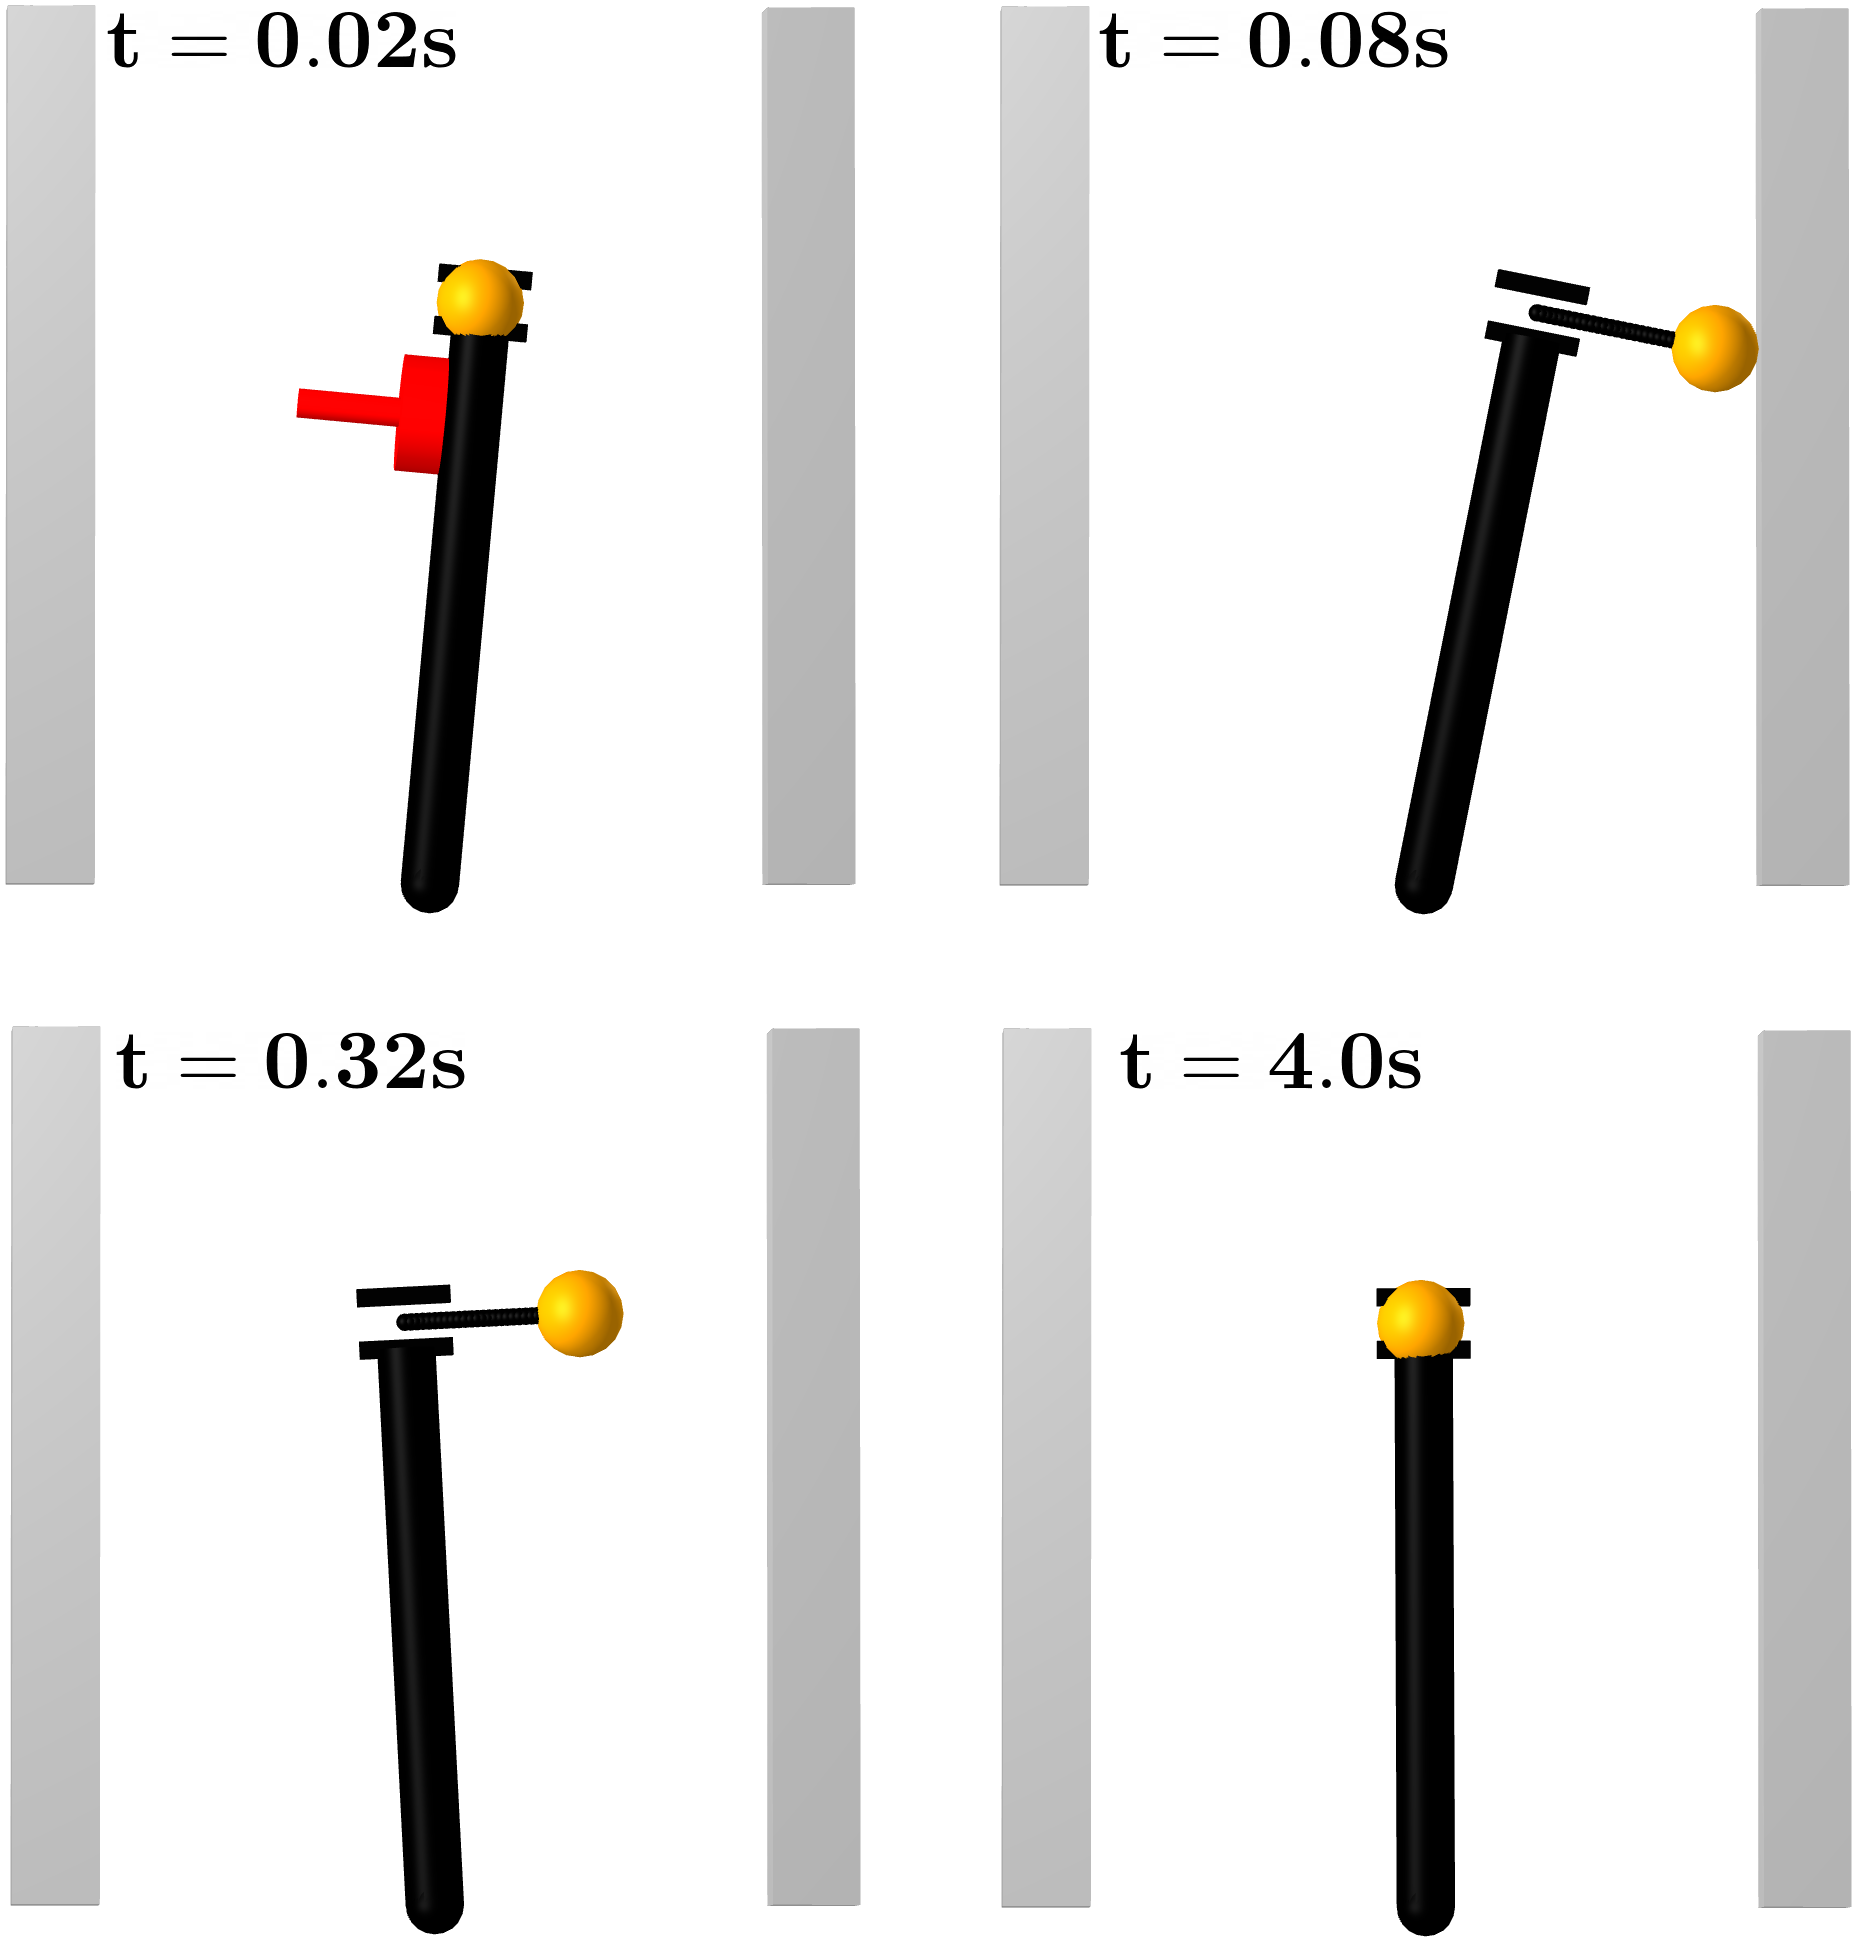
\includegraphics[width=.45\textwidth]{ci_pc/pushbot_figure_timings.png}
	\caption[Pushbot performing push recovery]{Pushbot performing push recovery. A disturbance (red) creates an impulse on the system and the policy generates a new contact sequence that extends the prismatic joint toward the right wall in order to make contact. After stabilizing, pushbot pushes against the wall, eventually breaking contact, in order to return to the nominal upright configuration.}
	\label{cipc_pushbot_push_recovery}
\end{figure}

We compare CI-MPC to a method that relies on a mixed-integer quadratic progam (MIQP) formulation \cite{bemporad1999control} applied to a simplified version of the PushBot (an inverted pendulum between two stiff walls). The MIQP minimizes a quadratic objective function subject to piecewise-linearized dynamics. Each linear dynamics domain corresponds to a single contact mode, and discrete decision variables are introduced to encode contact mode switches. Our CI-MPC approach is fast enough to be run online, however, this is not the case for the MIQP policy, as shown in Table \ref{cipc_pushbot_results}. Moreover, the complexity of the MIQP increases exponentially with the number of contact modes, making it an intractable approach for more complex systems. Warm-starting the MIQP \cite{marcucci2020warm} may make this approach more amenable to online optimization.

\begin{table}[H]
	\centering
	\caption[Numerical comparison between CI-MPC and MIQP policies for pushbot push recovery]{Comparison between CI-MPC and MIQP policies for pushbot example. For a fixed replanning rate of 25 Hz, we report the mean and standard deviations for the optimization times and compare this to the associated time budget (0.04 s). Both policies successfully regulate the system around the equilibrium point. However, the MIQP policy is slower than real-time, whereas the CI-MPC policy always remains within time budget, ensuring real-time performance.}
	
	\begin{tabular}{c c c}
		\toprule
		\textbf{Policy} &
		\textbf{Planning Time} &
		\textbf{Real-Time} \\
		\toprule
		CI-MPC & \boldmath $0.014 \pm 0.027 \mbox{\textbf{s}}$ \unboldmath & \checkmark \\ 
		MIQP   & $0.18  \pm 0.09$ s & \ding{53} \\ 
		\toprule
	\end{tabular}
	\label{cipc_pushbot_results}
\end{table}

\paragraph{Hopper.}
Inspired by the Raibert Hopper \cite{raibert1989dynamically}, we model a 2D hopping robot with $n_q = 4$ generalized coordinates: lateral and vertical positions, body orientation, and leg length, respectively; $m = 2$ controls: body moment, e.g., controlled with an internal reaction wheel, and leg force; and a single contact at the foot. 

The centroidal-dynamics modeling assumption we make---consistent with Raibert's work---is to locate the leg and foot mass at the body's center of mass. This results in a configuration-independent mass matrix and no bias term in the dynamics. 

The hopper is tasked with locomoting over unknown terrain. The CI-MPC policy uses a reference trajectory that is optimized with a flat surface and no incline. We compare our policy to the Raibert heuristic, which we similarly tune for flat ground and no incline. We observe that our policy is able to adapt to the varying surface heights that range from $0\mbox{-}24\:$cm and that the robot can slip multiple times and is able to recover while traversing steep inclines. We find that, when tuned well, the Raibert heuristic also works very well on terrains


\begin{figure}[H]
	\begin{center}
		\includegraphics[width=0.25\textwidth]{ci_pc/hopper_parkour_v1.png}
	\end{center}
	\caption[Hopper parkour]{Hopper performing parkour. The system tracks the body (orange) and foot (blue) reference trajectories while ascending three stairs before performing a front flip.}
	\label{cipc_hopper_parkour}
\end{figure}

Additionally, we task the hopper with climbing a staircase and executing a front flip (Fig. \ref{cipc_hopper_parkour}). This complex trajectory cannot be directly executed using the Raibert heuristic as it is not a periodic hopping gait. Our policy, however, successfully tracks this complex trajectory, illustrating the more general capabilities of CI-MPC. Results are summarized in Table \ref{cipc_hopper_results}.  

\begin{table}[H]
	\centering
	\caption[Comparison between CI-MPC and Raibert-heuristic policies for hopper locomotion and parkour]{Comparison between CI-MPC and the Raibert heuristic for a hopper system on 4 scenarios: flat, sinusoidal, and piecewise linear terrains; and a parkour stunt (Fig. \ref{cipc_hopper_parkour}). For each terrain profile, we report the number of hops achieved by the policy. For the parkour scenario, we report if the stunt is successfully completed.}
	
	\begin{tabular}{c c c c c}
		\toprule
		\textbf{Policy} &
		\textbf{Flat} &
		\textbf{Sinusoidal} &
		\textbf{Piecewise} &
		\textbf{Parkour}\\
		\toprule
		CI-MPC & $+100$ & $+100$ & $+100$ & \checkmark \\ 
		Raibert & $+100$ & $+100$ & $+100$ & \ding{53} \\ 
		\toprule
	\end{tabular}
	\label{cipc_hopper_results}
\end{table}

\paragraph{Planar quadruped.}
We model a planar quadruped with $n_q = 11$ configuration variables and $m = 8$ control inputs. The system has four contacts, one at each point foot. 

The quadruped is tasked with moving to the right over three different terrains: flat, sinusoidal, and piecewise-linear surfaces (Fig. \ref{cipc_quadruped_traj}). 



\begin{figure}[H]
	\centering
	\includegraphics[width=.48\textwidth]{ci_pc/quadruped.png}
	\caption[Planar quadruped walking over uneven terrain]{Planar quadruped walking over uneven terrain. The reference gait is optimized for flat ground.  Our CI-MPC policy, with orange center-of-mass and blue foot position trajectories, is able to adapt online to the unmodeled variation in terrain and track the reference trajectory.}
	\label{cipc_quadruped_traj}
\end{figure}

Additionally, we test the robustness of the CI-MPC policy by introducing model mismatch. We provide the policy with the nominal model of the quadruped while the simulator uses a quadruped with a $3$-kg payload, representing $25\%$ of its nominal mass. 

\begin{figure}[H]
	\centering
	\includegraphics[width=.45\textwidth]{ci_pc/quadruped_payload_cardboard_red.png}
	\caption[Planar quadruped locomotion with model mismatch]{Quadruped tracking a reference trajectory (red) while carrying an unmodeled $3$-kg payload. We depict the torso (orange) and front-left foot (blue) trajectories.}
	\label{cipc_quadruped_payload}
\end{figure}

Despite the unmodeled load, the policy successfully tracks the nominal gait with good performance. 

We note that the same CI-MPC policy was used across all quadruped experiments and no retuning was required to transfer from the nominal case (flat terrain, no payload) to more complex scenarios. Further, it is easy and intuitive to rapidly retune the policy in order to achieve improved tracking performance in the 
other scenarios.

\paragraph{Planar biped.}
We model a planar biped based on Pratt's Spring Flamingo \cite{pratt2000thesis} with $n_q = 9$ configuration variables and $m = 7$ control inputs. The system is modeled with four contact points, one at the toe and heel of each foot.

The biped is tasked with moving to the right over three different terrains: flat, sinusoidal, and piecewise-linear surfaces (Fig. \ref{cipc_biped_tracking}) using the same policy. 

\begin{figure}[H]
	\centering
	\includegraphics[width=.45\textwidth]{ci_pc/flamingo_ghost.png}
	\caption[Planar biped locomotion over unmodeled terrain]{Biped walking from left to right across flat (top), sinusoidal (middle), and piecewise linear (bottom) terrain using the same policy.}
	\label{cipc_biped_tracking}
\end{figure}

In Table \ref{cipc_biped_results}, we compare this to Pratt's policy \cite{pratt2000thesis}, which relies on a state-machine architecture and a number of proportional-derivative controllers. 

\begin{table}[H]
	\centering
	\caption[Comparison between CI-MPC and Pratt-heuristic policies for biped locomotion]{Comparison between CI-MPC and Pratt state-machine \cite{pratt2000thesis} policies for flamingo system on flat and inclined terrains. We report the number of steps taken by the robot on the flat terrain and compare the maximum incline traversed by our policy in simulation with reported results$^{\dagger}$ \cite{pratt1998intuitive}.}
	
	\begin{tabular}{c c c}
		\toprule
		\textbf{Policy} &
		\textbf{Flat} &
		\textbf{Incline}\\
		\toprule
		CI-MPC & $+100\phantom{^{\dagger}}$ & \boldmath $10$ \unboldmath \textbf{deg}. \\ 
		Pratt & $+100^{\dagger}$ &  $ 5^{\dagger}$  deg. \\ 
		\toprule
	\end{tabular}
	\label{cipc_biped_results}
\end{table}

Our CI-MPC policy---with no additional tuning---can easily walk on all of the terrains and reliably walks up inclines of up to ten degrees. Pratt reports that Spring Flamingo can only walk up inclines of five degrees without requiring the controllers to be re-tuned \cite{pratt1998intuitive}.

\paragraph{Monte Carlo.}
In order to assess the robustness of CI-MPC, we perform Monte Carlo analysis on two systems: the hopper and planar quadruped. The robots are tasked with tracking a reference gait and we initialize the systems with configurations that are randomly perturbed from the reference trajectory. We use 100 randomly sampled initial conditions for each system; the hopper recovers from significant orientation offsets and the quadruped is robust to large drops (Fig. \ref{cipc_monte_carlo}).

\begin{figure}[t]
	\begin{center}
		\includegraphics[width=0.45\textwidth]{ci_pc/hopper_2D_monte_carlo.png}
	\end{center}
	\begin{center}
		\includegraphics[width=0.45\textwidth]{ci_pc/quadruped_monte_carlo.png}
	\end{center}
	\caption[Monte Carlo CI-MPC policy test for hopper and planar quadruped]{Monte Carlo simulations of initial conditions for systems tracking a reference trajectory. 100 initial configurations are randomly sampled for a hopper (top) and quadruped (bottom). Perturbations from the reference initial configuration include large translations, tilts, and joint angles offsets. For all the samples, and both systems, the policy successfully recovers to the reference gait.}
	\label{cipc_monte_carlo}
\end{figure}

\subsection{Hardware}
In order to assess the robustness of CI-MPC, we perform Monte Carlo analysis on two systems: the hopper and planar quadruped. The robots are tasked with tracking a reference gait and we initialize the systems with configurations that are randomly perturbed from the reference trajectory. We use 100 randomly sampled initial conditions for each system; the hopper recovers from significant orientation offsets and the quadruped is robust to large drops (Fig. \ref{cipc_monte_carlo}).

\paragraph{Point-foot model.}
We utilize a simplified point-foot model of the quadruped that neglects leg dynamics. This model comprises 36 states which include the positions and velocities of the body and each foot. The orientation of the body is represented with Euler angles. The controls are three-dimensional forces applied to each foot, which is modeled as a point mass. Reference motions are generated offline with this model using contact-implicit trajectory optimization \cite{manchester2020variational}.

The primary reason for these modeling simplifications is to reduce the online computational requirement when evaluating the dynamics and their derivatives while still being able to reason about new contact sequences online. Importantly, unlike traditional convex quadratic programming policies \cite{bledt2017policy}, which assume a fixed contact sequence for the feet, our model is contact-implicit and enables new foot-step sequences to be generated online. 

\paragraph{Experimental setup.} 
A reference trajectory generated offline is tracked online using CI-MPC. A pre-tuned low-level controller generates joint torques that aim to match the forces specified by the policy that should be applied by each leg at the foot.
The CI-MPC policy is written in Julia and is precompiled in order to interface with an existing C++ low-level controller running at $1000$Hz. State feedback to the CI-MPC policy and the low-level controller is provided by a $1000$Hz Kalman filter which utilizes joint encoders, onboard IMU, and external motion-capture tracking to estimate the robot state. The policy, state estimator, and low-level controller run on a computer equipped with an Intel i9-12900KS CPU and 64GB of memory. The joint torque commands are sent to the quadruped via an ethernet connection. Additional information is provided in Table \ref{cipc_hardware_timing_table}.

\begin{table}[H]
	\centering
	\caption[Unitree Go1 quadruped hardware experiment details]{Hardware experiments with CI-MPC tracking different reference trajectories on a Unitree Go1 quadruped.}
	\begin{tabular}{c c c c}
		\toprule
		\textbf{Settings}  & \textbf{Trotting} & \textbf{Wall} & \textbf{Step}\\
		\toprule
		reference trajectory length & $0.8$ s & $19.75$ s & $7.0$ s \\
		reference time step & $0.05$ s & $0.05$ s & $0.05$ s\\
		policy planning horizon & $0.15$ s & $0.1$ s  & $0.1$ s\\
		policy rate & $100$ Hz & $100$ Hz & $100$ Hz\\
		\toprule
	\end{tabular}
	\label{cipc_hardware_timing_table}
\end{table}

\paragraph{Trotting.}
In this example, the specified behavior is trotting in place (Fig. \ref{cipc_quadruped_hardware_trot}). 

\begin{figure}[H]
	\centering
	\includegraphics[height=3.85cm]{ci_pc/cipc_quadruped_trot_push_blur.png}
	\caption[Unitree Go1 stable trotting while being pushed]{Unitree Go1 stable trotting while being pushed.}
	\label{cipc_quadruped_hardware_trot}
\end{figure}
The reference trajectory is 0.8 seconds and is repeated to form a continuous gait. The policy planning horizon is 0.10 seconds and the model uses a time discretization of 0.05 seconds. The policy runs at an average rate 100 Hz. 

A footstep sequence is shown in Fig. \ref{contact_sequence} for a scenario where a large disturbance is applied to the system during trotting.

\begin{figure}[H]
	\centering
	\includegraphics[width=1.00\textwidth, height=3.00cm]{ci_pc/contact_sequence.tikz}		\caption{Contact sequence for quadruped trotting. An external disturbance is applied to the system (red) and the policy is able to generate a new contact sequence online (black) that differs significantly from the reference plan (orange).}
	\label{contact_sequence}
\end{figure}

\paragraph{Wall stand.}
In this example, the specified behavior is transitioning from four feet on the ground to standing against the wall with two feet (Fig. \ref{cipc_quadruped_hardware_wall}). 

\begin{figure}[H]
	\centering
	\includegraphics[height=3.85cm]{ci_pc/cipc_quadruped_wallstand_blur.png}
	\caption[Unitree Go1 transitioning from ground to standing against a wall]{Unitree Go1 transitioning from ground to standing against a wall.}
	\label{cipc_quadruped_hardware_wall}
\end{figure}
The reference trajectory is 19.75 seconds. The policy planning horizon is 0.15 seconds and the model uses a time discretization of 0.05 seconds. The policy runs at an average rate of 100 Hz.

\paragraph{Step.}
In this example, the specified behavior has the quadruped place its right foot onto a step, followed by its left foot (Fig. \ref{cipc_quadruped_hardware_step}). 

\begin{figure}[H]
	\centering
	\includegraphics[height=3.85cm]{ci_pc/cipc_quadruped_step_blur.png}
	\caption[Unitree Go1 placing two feet onto a step]{Unitree Go1 placing two feet onto a step.}
	\label{cipc_quadruped_hardware_step}
\end{figure}
The entire reference trajectory is 7.0. The policy planning horizon is 0.1 seconds and the model uses a time discretization of 0.05 seconds. The policy runs at an average rate of 100 Hz.

\section{Limitations} \label{cipc_limitations}
We highlight important limitations including: approximations, contact model, and reliability, that should be considered before deploying CI-MPC policies.

\paragraph{Approximations.} 
For the online trajectory optimization problem, strategically approximated contact dynamics are utilized for planning. This enables expensive gradient computations and partial matrix factorizations to be performed in an offline stage, in order to substantially reduce online computation. In the examples, we find that short planning horizons, typically between $0.1$ and $0.25$ seconds, are sufficient. Despite the approximations introduced by these simplifications, in practice, the controls optimized for the fast contact dynamics work well in simulation and on hardware. However, it remains to be seen how well these approximations work for control of highly dynamic behaviours or scenarios that require longer planning horizons, particularly when deployed on hardware.

\paragraph{Contact model.} 
The physics of hard contact produces non-smooth and discontinuous gradients. With our custom interior-point method for the contact dynamics solver, we can efficiently compute smooth gradients in a principled way by exploiting intermediate results, parameterized by the central-path parameter. Hard contact is simulated by returning results from the contact dynamics solver with a central-path value $\kappa_{\mbox{sim}} = 1\mbox{e-}6$, whereas gradients are computed using intermediate results from the solve parameterized by $\kappa_{\mbox{grad}} \approx 1\mbox{e-}4$. 

During online optimization, we prioritize fast updates by solving the trajectory-tracking problem to coarse tolerances. In this context, imposing highly accurate contact physics would be wasteful in terms of computational resources. As a result, the central-path value for the planning dynamics is fixed to the gradient central-path value in order to reduce online computation. This selection was made to balance capturing accurate physics with producing usefully smooth gradients. Empirically, we observe that using these dynamics with slightly soften contact dynamics enhanced the convergence of the trajectory-tracking solver and likely enables the policy to more easily discover new contact sequences. Importantly, the allowed interpenetration with these tolerances is sub-millimeter---much less than allowed by MuJoCo's default settings---but, this raises the question, is simulation of perfectly hard contact actually necessary, or useful, for reliable planning and control of non-smooth systems?

\paragraph{Reliability.}
Generating high-quality reference trajectories is crucial for CI-MPC. Contact-implicit trajectory optimization \cite{posa2014direct, manchester2020variational} is a powerful tool for generating these trajectories. However, it is notorious for poor convergence properties, despite relying on robust large-scale constrained solvers for non-convex problems and even good warm starting. This unreliability makes online optimization generally impractical---motivating this work. Ultimately, for CI-MPC to be of practical value, generation of references trajectories, even in the offline setting, must be improved. This may be possible with specialized solvers for contact-implicit trajectory optimization \cite{howell2022calipso}, alternative rollout-based methods that leverage the reliability of one-step contact dynamics \cite{howell2022trajectory}, or learning-based approaches \cite{heess2017emergence}.

Additionally, our hardware experiments demonstrate the real-time capabilities of CI-MPC and its ability to be robust in many scenarios. However, in practice, we find that the classic convex MPC policy \cite{di2018dynamic} is significantly more robust for general locomotion because that policy has an additional online foothold selection strategy (the Raibert strategy). Adding this strategy to CI-MPC will likely increase its speed and reliability to match the performance of the baseline convex MPC policy. Performance will likely be improved further with a more efficient C/C++ implementation that utilizes multi-threading for parallel evaluations of the fast contact dynamics.

\section{Future Work} \label{cipc_future_work}
In summary, we have presented fast differentiable contact dynamics that can be utilized in an MPC framework that performs robust tracking for robotic systems that make and break contact with their environments. There remain many exciting avenues to explore in future work. First, it should be possible to perform higher-fidelity convex approximations of the contact dynamics that utilize second-order friction cones instead of its linearized approximation. This could enable tracking of highly dynamic behaviors that leverage accurate sliding contacts. Second, a natural extension of this work, which was focused on locomotion, is to the manipulation domain, potentially with quasi-static models, where control through contact is similarly an open problem, but where dynamics are slower and more amenable to online optimization. Third, in our hardware experiments, we utilized a simplified planning model for the quadruped. Similar point-contact models should extend to bipeds and humanoid systems, potentially even dexterous hands. Lastly, a library of template behaviors, comprising CI-MPC policies, could be composed to enable more diverse behavior online with a high-level agent composing templates in a task-and-motion-planning framework in order to generate complex long-horizon plans.

\section*{Acknowledgments}
This work was supported in part by Frontier Robotics, Innovative Research Excellence, Honda R\&D Co., Ltd, ONR award N00014-18-1-2830, NSF NRI award 1830402, and DARPA YFA award D18AP00064. Toyota Research Institute (TRI) provided funds to assist the authors with their research but this article solely reflects the opinions and conclusions of its authors and not TRI or any other Toyota entity.  
\chapter{Predictive Sampling}
We introduce MuJoCo MPC (\app{}), an open-source, interactive application and software framework for real-time predictive control, based on MuJoCo physics. \app{} allows the user to easily author and solve complex robotics tasks, and currently supports three shooting-based planners: derivative-based iLQG and Gradient Descent, and a simple derivative-free method we call Predictive Sampling. Predictive Sampling was designed as an elementary baseline, mostly for its pedagogical value, but turned out to be surprisingly competitive with the more established algorithms. This work does not present algorithmic advances, and instead, prioritizes performant algorithms, simple code, and accessibility of model-based methods via intuitive and interactive software. 

%\app{} is available at \url{https://github.com/deepmind/mujoco_mpc}, a video summary can be viewed at \url{https://dpmd.ai/mjpc}.

\vspace*{\fill}

\noindent Predictive Sampling: Real-time Behavior Synthesis with MuJoCo. Taylor A. Howell, Nimrod Gileadi, Saran Tunyasuvunakool, Kevin Zakka, Tom Erez, and Yuval Tassa. arXiv 2212.00541. 2022.

\pagebreak

\section{Introduction}

Model-based approaches form the foundation of classical control and robotics. Since Kalman's seminal work~\cite{kalman1960general}, the \emph{state} along with its dynamics and observation models has played a central role. 

The classical approach is being challenged by \textit{learning-based} methods, which forgo the explicit description of the state and associated models, letting internal representations emerge from the learning process \cite{lillicrap2015continuous, schulman2017proximal, salimans2017evolution, smith2022walk, rudin2022learning}. The flexibility afforded by learned representations makes these methods powerful and general, but the requirement for large amounts of data and computation makes them slow. In contrast, pure model-based methods, like the ones described below, can synthesize behavior in real time~\cite{tassa2014control}.

Since both approaches ultimately generate behavior by optimizing an objective, there is reason to believe they can be effectively combined. Indeed, well-known discrete-domain breakthroughs like AlphaGo~\cite{silver2016mastering} are predicated on combining model-based search and learning-based value and policy approximation. We believe the same could happen for robotics and control, and describe our thinking on how this might happen in the Discussion (Section \ref{ps_discussion}). However, before the community can rise to this challenge, a core problem must be overcome: Model-based optimization is difficult to implement, often depends on elaborate optimization algorithms, and is generally inaccessible. 

To address this deficit, we present \textit{\app{}}, an open-source interactive application and software framework for predictive control, based on MuJoCo physics~\cite{todorov2012mujoco}, which lets the user easily author and solve complex tasks using predictive control algorithms in real time. The tool offers implementations of standard derivative-based algorithms: iLQG (second-order planner) and Gradient Descent (first-order planner).  Additionally, it introduces \emph{Predictive Sampling}, a simple zero-order, sampling-based algorithm that works surprisingly well and is easy to understand. 

Importantly, the interactive simulation can be slowed down asynchronously, speeding up the planner with respect to simulation time. This means that behaviors can be generated on older, slower machines, leading to a democratization of predictive control tooling.

\app{} and Predictive Sampling advance our central goal of lowering the barriers to entry for predictive control in robotics research. An important secondary goal is to accelerate \textit{research velocity}. When tweaking a parameter, a researcher should not need to wait hours or minutes, but should receive instantaneous feedback -- which will measurably enhance their own cognitive performance~\cite{lu2022current}. We believe that flexible, interactive simulation with researcher-authored graphical user interface is not just a ``nice to have'', but a prerequisite for advanced robotics research.

\section{Background} \label{ps_background}

In this section we provide a general background on Optimal Control and Trajectory Optimization, then focus on Predictive Control and derivative-free optimization.

\paragraph{Optimal control.}
Optimal Control means choosing actions in order to minimize future costs (equivalently, to maximize future returns). A dynamical system with \emph{state} $\state \in \mathbf{R}^n$, which takes a user-chosen \emph{control} (or \emph{action}) $\control \in \mathbf{R}^m$, evolves according to the discrete-time\footnote{The continuous-time formulation is generally equivalent, we choose the discrete-time for notation simplicity.} dynamics,
\begin{equation}
	\state_{t+1} = f(\state_t, \control_t). 
	\label{ps_dynamics}
\end{equation}
The behavior of the system is encoded via the running cost $c : \mathbf{R}^n \times \mathbf{R}^m \rightarrow \mathbf{R}_+$, 
\begin{equation}
	\cost(\state_t, \control_t),
\end{equation}
a function of state and control, where explicit time-dependence can be realized by folding time into the state. Future costs (a.k.a \emph{cost-to-go} or \emph{value}), can be defined in several ways. The summation can continue to infinity, leading to the \emph{average-cost} or \emph{discounted-cost} formulations, favored in temporal-difference learning, which we discuss in Section \ref{ps_discussion}. Here we focus on the \emph{finite-horizon} formulation, whereby the optimization objective $\objective$ is given by:
\begin{equation}
	\objective(\state_{0:T}, \control_{0:T}) = \sum_{t=0}^{T} \cost(\state_t, \control_t). \label{ps_objective}
\end{equation}

\paragraph{Trajectory optimization.}
Solving the finite-horizon optimal control problem (\ref{ps_dynamics}, \ref{ps_objective}), i.e., optimizing a fixed-length trajectory, is commonly known as \emph{planning} or \emph{trajectory optimization}. These algorithms \cite{von1992direct, betts1998survey} have a rich history reaching back to the Apollo Program \cite{manned1971apollo,smith1967trajectory}. An important distinction can be made between two classes of algorithms:
\begin{itemize}
	\item \emph{Direct} or \emph{simultaneous} methods have both states and controls as decision variables and enforce the dynamics~\eqref{ps_dynamics} as constraints. These methods (e.g., \cite{stryk1993numerical}) specify a large, sparse optimization problem, which is usually solved with general-purpose software \cite{wachter2006implementation, gill2005snopt}. They have the important benefit that non-physically-realizable trajectories can be represented, for example in order to clamp a final state, without initially knowing how to get to it.
	\item \emph{Shooting} methods like Differential Dynamic Programming \cite{jacobson1970differential} use only the controls $\control_{0:T}$ as decision variables and enforce the dynamics via forward simulation. In the shooting approach only physically-realizable trajectories can be considered, but they benefit from the reduced search space and from the optimizer not having to enforce the dynamics. The latter benefit is especially important for stiff systems like those with contact, where the difference between a physical and non-physical trajectory can be very small\footnote{For example, consider the physical scenario of a free rigid box lying flat on a plane under gravity, and then consider the non-physical scenario of the same box hovering above the plane or penetrating it by a few microns.}. Unlike \emph{direct} methods which require dynamics derivatives, shooting methods can employ derivative-free optimization, as discussed below.
\end{itemize}

\paragraph{Predictive control.}

The key idea of Predictive Control, invented in the late 60s and first published in \cite{richalet1978model}, is to use trajectory optimization in \emph{real-time} as the system dynamics are evolving. This class of algorithm has been successfully deployed in numerous real-world settings including: chemical and nuclear process control \cite{na2003model, lopez2013fast}, navigation for autonomous vehicles \cite{falcone2007predictive}, and whole-body control of humanoid robots \cite{kuindersma2016optimization}.

In the real-time setting, the current state $\state$ needs to be estimated or measured, and the trajectory optimizer is required to return a set of optimal or near-optimal controls for the finite-horizon (here often called the \emph{receding horizon}) problem, starting at $\state$. We use $\plan$ to denote the \emph{plan}, the finite-horizon policy. In the context of shooting methods $\plan = \control_{0:T}$, though as we discuss later, in some cases it can be re-parameterized, rather than using the discrete-time control sequence directly. Predictive control is best thought of in terms of two asynchronous processes, the \emph{agent} and the \emph{planner}:

\begin{algorithm}[H]
	\caption{Predictive Control (asynchronous)}\label{ps_predictive_control}
	\textbf{Agent}: (repeat)
	\begin{algorithmic}[1]
		\State Read the current action $\control$ from the \emph{nominal} plan $\plan$, apply it to the controlled system.
	\end{algorithmic}
	\textbf{Planner}: (repeat)
	\begin{algorithmic}[1]
		\State Measure the current state $\state$.
		\State Using the nominal $\plan$ to warm start, optimize the finite-horizon objective $\objective$.
		\State Update $\plan$.
	\end{algorithmic}	
\end{algorithm}

Predictive Control has the following notable properties:
\begin{itemize}
	\item Faster computation improves performance. The reason for this is clear, the more optimization steps the planner can take in one unit of time, the better the optimized control sequences will be.
	\item Warm starting has a large beneficial effect. By reusing the plan from the previous planning step, the optimizer only needs to make small modifications in order to correct for the changes implied by the new state. Warm starting also leads to an amortization of the optimization process across multiple planning steps.
	\item The optimization is not required to converge, only to improve, see Section \ref{ps_discussion}.
	\item Tasks with a behavior timescale much longer than the planning horizon $T$ are often still solvable, though this property is task dependent.
	\item Predictive controllers can easily get stuck in local minima, especially those using derivatives. This is due to the myopic nature of the optimization, and can be addressed by terminating the rollout with a value function approximation, see Section \ref{ps_future_work}.
\end{itemize}

\paragraph{Derivative-free optimization.}
One of the main reasons for our initial focus on shooting methods is their ability to make use of derivative-free optimization, also known as \emph{sampling-based} optimization~\cite{audet2017derivative}. Despite not leveraging problem structure or gradient information, this class of algorithms can discover complex behaviors \cite{salimans2017evolution, mania2018simple}.

Sampling-based methods maintain a search distribution over policy parameters and evaluate the objective at sampled points in order to find an improved solution. Popular algorithms include: random search \cite{matyas1965random}, genetic algorithms \cite{holland1992genetic}, and evolutionary strategies \cite{rechenberg1973evolutionsstrategie}, including CMA-ES \cite{hansen2001completely}. 

This class of algorithms has a number of desirable properties. First, because derivative information is not required, they are well-suited for tasks with non-smooth and discontinuous dynamics. Second, these methods are trivially parallelizable.

Sampling-based methods have been used in the predictive control context, but not very widely. Notable exceptions are H{\"a}m{\"a}l{\"a}inen's work \cite{hmlinen2014online, hmlinen2015online}, which is an early precursor to \app{}, and the oeuvre of Theodorou including~\cite{williams2017model} and related papers. While these methods are usually considered to be sample inefficient, we explain below why, specifically in the predictive control context, they can be surprisingly competitive.

\section{MuJoCo MPC (\app{})} \label{ps_mujoco_mpc}

We introduce \app{}, an open-source interactive application and software framework for predictive control, that lets the user easily synthesize behaviors for complex systems using predictive control algorithms in real time. Behaviors are specified by simple, composable objectives that are risk-aware. The planners, including: Gradient Descent, Iterative Linear Quadratic Gaussian (iLQG), and Predictive Sampling are implemented in C++ and extensively utilize multi-threading for parallel rollouts. The framework is asynchronous, enabling simulation slow-down and emulation of a faster controller, allowing this tool to run on slow machines. An intuitive graphical user interface enables real-time interactions with the environment and the ability to modify task parameters, planner and model settings, and to instantly see the effects of the modifications. The tool is available at:
\begin{center}
\url{https://github.com/deepmind/mujoco_mpc}
\end{center}

\subsection{Physics simulation}
We build \app{} using the API of the open-source physics engine MuJoCo \cite{todorov2012mujoco}.  MuJoCo is a good infrastructure for an interactive framework for robotics algorithms for two main reasons: first, MuJoCo supports simulating multiple candidate future trajectories in parallel by offering a thread-safe API, which maximizes the utilization of modern multi-core CPU architectures; second, MuJoCo affords faster-than-real-time simulation of high-dimensional systems with many contacts --- for example, the humanoid (a 27-DoF system) can be simulated 4000 times faster than real-time on a single CPU thread.

\subsection{Objective}
\app{} provides convenient utilities to easily design and compose costs in order to specify an objective \eqref{ps_objective}; as well as automatically and efficiently compute derivatives.

\paragraph{Costs.}

We use a ``base cost'' of the form:
\begin{equation}
	\label{ps_riskfreecost}
	\precost(\state, \control) = \sum_{i = 0}^M w_i \cdot \text{n}_i\big(\residual_i(\state, \control)\big).
\end{equation}
This cost is a sum of $M$ terms, each comprising:
\begin{itemize}
	\item A nonnegative weight $w \in \mathbf{R}_{+}$ determining the relative importance of this term.
	\item A twice-differentiable norm $\text{n}(\cdot) : \mathbf{R}^p \rightarrow \mathbf{R}_+$, which takes its minimum at $0^p$.
	\item The residual $\residual \in \mathbf{R}^p$ is a vector of elements that are ``small when the task is solved''.%Residuals are implemented as custom MuJoCo sensors.
\end{itemize}

\paragraph{Risk sensitivity.}

We augment the base cost \eqref{ps_riskfreecost} with a risk-aware exponential scalar transformation, $\rho : \mathbf{R}_+ \times \mathbf{R} \rightarrow \mathbf{R}$, corresponding to the classical risk-sensitive control framework \cite{jacobson1973optimal, whittle1981risk}. The final running cost $\cost$ is given by:
\begin{equation}
	\cost(\state, \control) = \rho(\precost(\state, \control) ; R) = \frac{e^{R\cdot \precost(\state, \control)} - 1}{R}.
	\label{ps_riskfunc}
\end{equation}
The scalar parameter $R \in \mathbf{R}$ denotes risk-sensitivity. $R=0$ (the default) is interpreted as risk-neutral, $R>0$ as risk-averse, and $R<0$ as risk-seeking.
The mapping $\rho$ (see Figure \ref{ps_riskfig})

\begin{figure}[H]
	\centering
	\includegraphics[height=7.0cm]{predictive_sampling/risk.tikz}
	\caption[Risk transformation]{Risk transformation $\rho(l ; R)$. The function is evaluated between $0$ and $1$ for different values of the risk parameter $R$.}
	\label{ps_riskfig}
\end{figure}

has the following properties:

\begin{itemize}
	\item Defined and smooth for any $R$.
	\item If $R=0$, is the identity $\rho(\precost; 0) = \precost$ (in the limit).
	\item Zero is a fixed point: $\rho(0; R) = 0$.
	\item The derivative at 0 is 1: $\partial \rho(0; R) / \partial \precost = 1$.
	\item Non-negative: If $\precost \geq 0$ then $\rho(\precost; R) \geq 0$.
	\item Monotonic: $\rho(\precost; R) > \rho(z; R)$ if $\precost > z$.
	\item If $R<0$ then $\rho$ is bounded: $\rho(\precost; R) < - \frac{1}{R}$.
	\item $\rho(\precost;R)$ carries the same units as $\precost$.
\end{itemize}

Note that for negative $R$, the transformation $\rho$ creates costs that are similar to the bounded rewards commonly used in reinforcement learning. For example, when using the quadratic norm $\text{n}(r) = r^T W r$ for some SPD matrix $W=\Sigma^{-1}$ and a risk parameter $R=-1$, we get an inverted-Gaussian cost $\cost=1 - e^{-r^T \Sigma^{-1} r}$, whose minimization is equivalent to maximum-likelihood maximization of the Gaussian. This leads to the interesting interpretation of the bounded rewards commonly used in RL as \emph{risk-seeking}. We do not investigate this relationship further in this paper.

\paragraph{Derivatives.}
MuJoCo provides a utility for computing finite-difference (FD) Jacobians of the dynamics, which is efficient in two ways. First, by avoiding re-computation where possible, for example when differencing w.r.t. controls, quantities that depend only on positions and velocities are not recomputed. Second, because FD computational costs scale with the dimension of the \emph{input}, outputs can be added cheaply. MuJoCo's step function $x_{t+1}, r_{t+1} = f(x_t, u_t)$, computes both the next state $x_{t+1}$ and sensor values $r_{t+1}$, defined in the model. Because the FD approximation of the Jacobians,
\begin{equation}
	\frac{\partial x_{t+1}}{\partial x_t}, \frac{\partial x_{t+1}}{\partial u_t}, \frac{\partial r_{t+1}}{\partial x_t}, \frac{\partial r_{t+1}}{\partial u_t},
\end{equation}
scales like the combined dimension of $x_t$ and $u_t$, adding more sensors $r_{t+1}$ is effectively ``free''. \app{} automatically and efficiently computes cost derivatives as follows.
\paragraph{Gradients.} Cost gradients are computed with:
\begin{subequations}
	\begin{align}
		\frac{\partial \cost}{\partial \state} &= e^{R \precost} \frac{\partial \precost}{\partial \state}=e^{R \precost}\sum \limits_{i = 0}^M w_i \frac{\partial \text{n}_i}{\partial r} \frac{\partial r_i}{\partial \state}, \\
		\frac{\partial \cost}{\partial \control} &= e^{R \precost} \frac{\partial \precost}{\partial \control} = e^{R \precost}\sum \limits_{i = 0}^M w_i \frac{\partial \text{n}_i}{\partial r} \frac{\partial r_i}{\partial \control}.
	\end{align}
\end{subequations}
The norm gradients, $\partial \text{n} / \partial r$, are computed analytically.

\paragraph{Hessians.}

Second-order derivatives use the Gauss-Newton approximation, ignoring second derivatives of $\residual$:
\begin{subequations}
	\begin{align}
		\frac{\partial^2 \cost}{\partial \state^2} \approx&\,  e^{R \precost} \left[ \sum \limits_{i = 0}^M w_i {\frac{\partial r_i}{\partial \state}}^T\frac{\partial^2 \text{n}_i}{\partial r^2} \frac{\partial r_i}{\partial \state} + R {\frac{\partial \precost}{\partial \state}}^T \frac{\partial \precost}{\partial \state} \right], \\
		\frac{\partial^2 \cost}{\partial \control^2} \approx& \, e^{R \precost} \left[ \sum \limits_{i = 0}^M w_i {\frac{\partial r_i}{\partial \control}}^T\frac{\partial^2 \text{n}_i}{\partial r^2} \frac{\partial r_i}{\partial \control}  + R {\frac{\partial \precost}{\partial \control}}^T \frac{\partial \precost}{\partial \control} \right],\\
		\frac{\partial^2 \cost}{\partial \state \partial \control} \approx& \, e^{R \precost} \left[ \sum \limits_{i = 0}^M w_i {\frac{\partial r_i}{\partial \state}}^T \frac{\partial^2 \text{n}_i}{\partial r^2} \frac{\partial r_i}{\partial \control} + R {\frac{\partial \precost}{\partial \state}}^T \frac{\partial \precost}{\partial \control} \right].
	\end{align}
\end{subequations}
The norm Hessians, $\partial^2 \text{n}/\partial r^2$, are computed analytically.

\subsection{Splines}

As we explain below, planners like iLQG require the \emph{direct} control-sequence representation $\control_{0:T}$ due to the requirements of the Bellman Principle. Without this constraint, controls can be ``compressed'' into a lower-dimensional object. There are many ways to do this, we picked the simplest: splines. Action trajectories are represented as a time-indexed set of knots, or control-points, parameterized by a sequence of monotonic time points $\tau_{0:P}$ and parameter values $\theta_{0:P}$, where we use the shorthand $\theta = \theta_{0:P}$. Given a query point $\tau$, the evaluation of the spline is given by:
\begin{equation}
	\control = s\big(\tau; (\tau_{0:P}, \theta) \big).
\end{equation}
We provide three spline implementations: traditional cubic Hermite splines, piecewise-linear interpolation, and zero-order hold. See (Fig. \ref{ps_spline}) for an illustration.

\begin{figure}[H]
	\centering
	\includegraphics[width=0.75\columnwidth,height=5.0cm]{predictive_sampling/spline.tikz}
	\caption[Spline representation]{Time-indexed spline representation of the controls. Parameter points (black) utilized to construct: zero (magenta), linear (orange), and cubic (blue) interpolants.}
	\label{ps_spline}
\end{figure}

The main benefit of compressed representations like splines is that they reduce the search space. They also smooth the control trajectory, which is often desirable. Spline functions belong to the class of linear bases, which includes the Fourier basis and orthogonal polynomials. These are useful because they allow easy propagation of gradients from the direct representation $\partial \plan$  back to the parameter values $\partial \theta$. In our case this amounts to computing:
\begin{equation}\label{ps_splinederiv}
	\frac{\partial s}{\partial \theta},
\end{equation}
which has a simple analytic formula (see code for details). Unlike other linear bases, splines have the convenient property that bounding the values $\theta$ also bounds the spline trajectory. This is exactly true for the zero and linear interpolations, and mostly-true for cubic splines. Bounding is important as most physical systems clamp controls to bounds, and there is no point searching outside of them. Expressions for cubic, linear and zero interpolations are provided in Appendix A.


\subsection{Planners}
\app{} includes two derivative-based planners. 

\paragraph{iLQG.}

The iLQG\footnote{Equivalently, ``iLQR'', since we don't make use of the noise-sensitive term for which iLQG was originally developed~\cite{li2004iterative}. We keep the name ``iLQG'' due to its provenance.} planner~\cite{tassa2012synthesis}, a Gauss-Newton approximation of the DDP algorithm~\cite{jacobson1970differential}, utilizes first- and second-order derivative information to take an approximate Newton step over the open-loop control sequence $\control_{0:T}$ via dynamic programming \cite{kalman1964lqr}, producing a time-varying linear feedback policy:
\begin{equation}
	\control_t = \bar{\control}_t + K_t (\state_t - \bar{\state}_t) + \alpha k_t \label{ps_ilqg_feedback_policy}.
\end{equation}
The \emph{nominal}, or current best trajectory, is denoted with overbars ($\bar{\phantom{x}}$), $K$ is a feedback gain matrix, and $k$ is an improvement to the current action trajectory. A parallel line search over the step size $\alpha \in [\alpha_{\textrm{min}}, 1]$ is performed to find the best improvement. Additional enhancements include a constrained backward pass \cite{tassa2014control} that enforces action limits and adaptive regularization. The details of iLQG are too involved to restate here, we refer the reader to the references above for details.

\begin{algorithm}[H]
	\caption{iLQG}\label{ps_ilqg_algorithm}
	\begin{algorithmic}[1]
		\Require initial state $\state_0$, nominal plan $\plan=\control_{0:T}$
		\State Roll out nominal trajectory from $\state_0$ using $\plan$
		\State Compute action improvements and feedback policy using Dynamic Programming.
		\State Roll out parallel line search with feedback policy \eqref{ps_ilqg_feedback_policy}.
		\State Best actions are new nominal actions.
	\end{algorithmic}
\end{algorithm}

\paragraph{Gradient descent.}

This first-order planner, known as Pontryagin's Maximum Principle \cite{mangasarian1966sufficient}, utilizes gradient information to improve action sequences, here represented as splines. The gradient of the total return is used to update the spline parameters, using a parallel line search over the step size $\alpha \in [\alpha_{\textrm{min}}, \alpha_{\textrm{max}}]$:
\begin{equation} \label{ps_linesearch}
	\theta \leftarrow \theta - \alpha \frac{\partial J}{\partial \theta}.
\end{equation}
The total gradient is given by:
\begin{equation}\label{ps_paramderivs}
	\frac{\partial J}{\partial \theta} = \frac{\partial J}{\partial \plan} \frac{\partial \plan}{\partial \theta},
\end{equation}
where the spline gradient $\partial \plan/\partial \theta$ is given by \eqref{ps_splinederiv}, while $\partial J/\partial \plan$ is computed with the Maximum Principle. Letting $\lambda$ denote the \emph{co-state}, the gradients with respect to $\control$ are given by:
\begin{subequations}\label{ps_pontryagin}
	\begin{align}
		\lambda_{j} &= \frac{\partial c}{\partial \state_j} + \Bigl(\frac{\partial f}{\partial \state_j}\Bigr)^T\lambda_{j+1}, \\
		\frac{\partial \objective}{\partial \control_j} &= \frac{\partial c}{\partial \control_j} + \Bigl(\frac{\partial f}{\partial \control_j}\Bigr)^T\lambda_{j+1}.
	\end{align}
\end{subequations}
The primary advantage of this first-order method compared to a computationally more expensive method like iLQG is that optimization is performed over the smaller space of spline parameters, instead of the entire (non-parametric) sequences of actions.

\begin{algorithm}[H]
	\caption{Gradient Descent}\label{ps_gradient_descent_algorithm}
	\begin{algorithmic}[1]
		\Require initial state $\state_0$, nominal plan $\plan(\theta)$
		\State Roll out nominal from $\state_0$ using $\plan(\theta)$
		\State Compute $\partial \objective/\partial \plan$ with \eqref{ps_pontryagin}
		\State Compute $\partial \objective/\partial \theta$ with \eqref{ps_paramderivs}
		\State Roll out parallel line-search with \eqref{ps_linesearch}
		\State Pick the best one: $\theta \leftarrow \mbox{arg min} \bigl(\objective(\theta^{(i)})\bigr)$
	\end{algorithmic}
\end{algorithm}

\paragraph{Predictive Sampling.}

This is a trivial, zero-order, sampling-based Predictive Control method that works well and is easy to understand. Designed as an elementary baseline, this algorithm turned out to be surprisingly competitive with the more elaborate derivative-based algorithms.

\paragraph{Algorithm.} A nominal sequence of actions, represented with spline parameters, is iteratively improved using random search \cite{matyas1965random}. At each iteration, $N$ candidate splines are evaluated: the nominal itself and $N-1$ noisy samples from a Gaussian with the nominal as its mean and fixed standard deviation $\sigma$. After sampling, the actions are clamped to the control limits by clamping the spline parameters $\theta$. Each candidate's total return is evaluated and the nominal is updated with the best candidate. See Algorithm \ref{ps_predictive_sampling_algorithm} and pseudocode in Appendix C. Predictive Sampling is not innovative or performant, but is presented as a simple baseline, see Discussion below.

\begin{algorithm}[H]
	\caption{Predictive Sampling}\label{ps_predictive_sampling_algorithm}
	\textbf{Parameters:} $N$ rollouts, noise scale $\sigma$
	\begin{algorithmic}[1]
		\Require initial state $\state_0$, nominal plan $\plan(\theta)$
		\State Get $N\!-\!1$ samples $\theta_i \sim \mathcal{N}(\theta, \sigma^2)$
		\State Including $\theta$, roll out all $N$ samples from $\state_0$
		\State Pick the best one: $\theta \leftarrow \mbox{arg min} \bigl(\objective(\theta^{(i)})\bigr)$
	\end{algorithmic}
\end{algorithm}

Our repository \url{https://github.com/deepmind/mujoco_mpc} includes a notebook that implements Predictive Sampling with easy-to-understand Python code.

\section{Results} \label{ps_results}

We provide a short textual description of our graphical user interface (GUI) for three example tasks. They are best understood by viewing the associated video at \url{https://dpmd.ai/mjpc} or better yet, by downloading the software and interacting with it. 

\subsection{Graphical user interface}

The MJPC GUI, shown and described in Fig. \ref{ps_gui}, provides an interactive simulation environment, as well as modules containing live plots and parameters that can be set by the researcher. 

\begin{figure}[H]
	\centering
	\includegraphics[width=.95\textwidth]{predictive_sampling/gui.png}%
	\caption[MuJoCo MPC graphical user interface]{MuJoCo MPC graphical user interface. The left tab includes modules for Tasks and the Agent. In the Task module, models are selected from a drop-down menu and the risk value is set; cost weights and residual parameters are specified with interactive sliders. The Agent module provides access to a drop-down menu for planners, settings, and switches that toggle the planner and controller. The right tab includes simulation readings and predictions for the cost, including individual terms, and actions. Live, planner-specific information and various compute time results are shown below. Traces of the current policy and sampled trajectories are visualized and the user can interactively pause or slow down the simulation and apply external forces and moments to the system.}%
	\label{ps_gui}
\end{figure}

The intuitive interface makes policy design easy by enabling the researcher to interactively change cost parameters or planner settings and immediately see the results in both the simulation environment and live plots, allowing fast debugging and an enhanced understanding of the factors that influence behavior.

\subsection{Examples}

In the following examples, we demonstrate the ability to synthesize complex locomotion and manipulation behaviors for a variety of high-dimensional systems in simulation on a single CPU. Further, we demonstrate that the behaviors are robust to disturbances and mismatch between the simulation and planning model, and can adapt extremely quickly in new scenarios. For all of the examples, the total planning time for a single update is between 1 and 20 milliseconds. We highlight three examples below and provide additional examples with the software. Experimental details for objectives and planner settings are found in the Appendix B.

\paragraph{Humanoid.}
This 27-DOF human-like system, from DeepMind Control Suite \cite{tunyasuvunakool2020dm_control}, has 21 actions and is tasked with standing. The system can be initialized on the floor and quickly stands in a manner that is robust to large disturbances. If a sufficiently large disturbance knocks the humanoid onto the floor, the system will stand back up (Fig. \ref{ps_humanoid_standing}).

\paragraph{Quadruped.}
A Unitree A1 quadruped \cite{unitree2022a1}, from MuJoCo Menagerie \cite{menagerie2022github}, exhibits agile behavior to traverse uneven terrain which includes walking over a steep slope. On slower machines, the quadruped often struggles to ascend. In this scenario, the simulation slow down can be effectively utilized to provide the planner with addition simulation time to plan a successful climb. The system is also capable of rolling off its back and standing up (Fig. \ref{ps_quadruped}). In order to perform long-horizon tasks like continuously navigating the terrain, a series of target poses are set. Once a goal is reached, an automatic transition occurs and the next target is set. 

\paragraph{Hand.}
A Shadow Hand \cite{tuffield2003shadow}, also from MuJoCo Menagerie, performs in-hand manipulation of a cube to a desired orientation (Fig. \ref{ps_hand}), where this goal can be set by the researcher in real-time by interactively setting the target orientation. In-hand reorientation---a high-DoF system with complex contact dynamics---is considered difficult to solve~\cite{chen2022system} and to the best of our knowledge has not previously been solved from scratch, in real time.

\begin{figure}[H] % <---
	\captionsetup[subfigure]{justification=centering}
	\begin{subfigure}{0.99\textwidth}
		\centering
		\includegraphics[width=.175\textwidth]{predictive_sampling/humanoid_1.png}%
		\includegraphics[width=.175\textwidth]{predictive_sampling/humanoid_2.png}%
		\includegraphics[width=.175\textwidth]{predictive_sampling/humanoid_3.png}%
		\includegraphics[width=.175\textwidth]{predictive_sampling/humanoid_4.png}%
		\includegraphics[width=.175\textwidth]{predictive_sampling/humanoid_5.png}%
		\caption{Humanoid standing up off the floor.}
		\label{ps_humanoid_standing}
		\vspace*{7.5mm} % <--- 
	\end{subfigure}
	\begin{subfigure}{0.99\textwidth}
		\centering
		\includegraphics[width=.175\textwidth]{predictive_sampling/quadruped_up1.png}%
		\includegraphics[width=.175\textwidth]{predictive_sampling/quadruped_up2.png}%
		\includegraphics[width=.175\textwidth]{predictive_sampling/quadruped_up3.png}%
		\includegraphics[width=.175\textwidth]{predictive_sampling/quadruped_up4.png}%
		\includegraphics[width=.175\textwidth]{predictive_sampling/quadruped_up5.png}%
		\caption{Quadruped rolling off its back to stand up.}
		\label{ps_quadruped}
		\vspace*{7.5mm} % <---
	\end{subfigure}
	\begin{subfigure}{0.98\textwidth}
		\centering
		\includegraphics[width=.225\textwidth]{predictive_sampling/hand_1.png}%
		\includegraphics[width=.225\textwidth]{predictive_sampling/hand_2.png}%
		\includegraphics[width=.225\textwidth]{predictive_sampling/hand_3.png}%
		\includegraphics[width=.225\textwidth]{predictive_sampling/hand_4.png}%
		\caption{Hand manipulating a cube to a goal orientation.}
		\label{ps_hand}
	\end{subfigure}
	\caption[Behaviors generated with MuJoCo MPC]{Behaviors generated with MuJoCo MPC. Time progresses left to right.}
	\label{ps_examples}
\end{figure}

\section{Discussion} \label{ps_discussion}
The thrust of this paper is to make predictive control accessible via customizable, interactive, open-source tooling. We believe that responsive, GUI-based tools are a prerequisite for accelerated robotics research, and that due to their importance, these tools should be modifiable and the inner workings transparent to the researcher. We hope that our \app{} project will be embraced by the community, and look forward to improving and extending it together.

\subsection{Predictive Sampling}
The effectiveness of this simple method suggests that fast, approximate optimization can be competitive with more sophisticated methods which return better solutions but at a lower rate. Does the higher planning rate completely explain this surprising effectiveness? We believe there is another, subtler reason. Predictive Control is not well-described by the tenets of traditional optimization. For example, it usually makes no sense to take more than one step of optimization. Once a single iteration is complete, it is more important to measure a new value of the state and re-plan, than it is to continue to converge to the minimum of an already-outdated problem. The constant shifting of the optimization landscape makes Predictive Control a \emph{qualitatively different problem}, more like surfing than mountain climbing. The goal is not to find the minimum, but to \emph{remain in the basin-of-attraction of the minimum}. This is a different, weaker criterion, at which simple algorithms fair better than when measured by the traditional yardstick of convergence.

To be clear, Predictive Sampling is not a novel algorithm; instead, it is a baseline. A corner-case of many existing methods, it can variously be described as ``MPPI with infinite temperature'',  ``CEM with a non-adaptive distribution'' or just ``trivial random search''. Better algorithms exist, but none are so easy to describe or implement. We are introducing Predictive Sampling not because it is good, but because it is \emph{not good}. It is the simplest possible sampling-based shooting method, and therefore establishes a \emph{lower bound} for performance baselines.

\subsection{Use cases} \label{ps_current}

Before we discuss limitations and their possible resolutions, it is worth asking how can \app{} be used \emph{now}, as it is described above?
\begin{enumerate}
	\item \textbf{Task design}. \app{} makes it easy to add new tasks, expose task parameters to the GUI, and quickly generate the desired behavior. The task can then be re-implemented in any other framework of choice. While we have not yet implemented time-dependent tasks, it is possible and easy; we expect \app{} to work especially well for motion-tracking tasks.
	\item \textbf{Data generation}. \app{} can be used to generate data for learning-based approaches, i.e., it can act like an ``expert policy''. In this context, it is often the case that the model and task from which the data is generated do not have to exactly match the one used by the learner, and the data can likely be useful for a wide range of setups.
	\item \textbf{Predictive Control research}. For researchers interested in Predictive Control itself, \app{} provides an ideal playground. \app{} can switch planners on-the-fly, and its asynchronous design affords a fair comparison by correctly accounting for and rewarding faster planners.
\end{enumerate}

\subsection{Limitations and future work} \label{ps_future_work}

\paragraph{Can only control what MuJoCo can simulate.} This is a general limitation of Predictive Control and is in fact stronger since one can only control what can be simulated \emph{much faster than real-time}. For example, it is difficult to imagine any simulation of a very-high-DOF system, like fluid, cloth or soft bodies advancing so fast. One solution is improved simulation using a combination of traditional physics modeling and learning, e.g., \cite{ladicky2017physics}. Another possibility is to entirely learn the dynamics from observations. This approach, often termed Model Based Reinforcement Learning is showing great promise \cite{heess2015learning, nagabandi2020deep, wu2022daydreamer}. We would recommend that where possible, when attempting Predictive Control using learned dynamics models, a traditional simulator be employed as a fallback as in \cite{schrittwieser2020mastering}, to disambiguate the effects of modeling errors. 

\paragraph{Myopic.} The core limitation of Predictive Control is that it is \emph{myopic} and cannot see past the fixed horizon. This can be ameliorated in three conceptually straightforward ways:
\begin{enumerate}
	\item \textbf{Learned policies}. By adding a learned policy, information from past episodes can propagate to the present via policy generalization~\cite{byravan2021evaluating}. This approach is attractive since it can only \emph{improve} performance: when rolling out samples, one also rolls out the proposal policy. If the rollout is better, it becomes the new nominal. A learned policy is also expected to lead to more stereotypical, periodic behaviors, which are important in locomotion. 
	\item \textbf{Value functions}. Terminating the rollout with a learned value function which estimates the remaining cost-to-go is the obvious way by which to increase the effective horizon. Combining learned policies and value functions with model-based search would amount to an ``AlphaGo for control''~\cite{silver2016mastering, springenberg2020local}.
	\item \textbf{High-level agent}. A predictive controller could be used as the low-level module in a hierarchical control setup. In this scenario, the actions of the high-level agent have the semantics of setting the cost function of the predictive controller. The predictive controller remains myopic while the high-level agent contains the long-horizon ``cognitive'' aspects of the task. A benefit of this scenario is that the high-level actions have a much lower frequency than required for low-level control (e.g., torques).
\end{enumerate}

\paragraph{Hardware.} \app{} is aimed at robotics research, which raises the question, can it be used to control hardware?
\begin{enumerate}
	\item \textbf{Transfer learning}. As mentioned in \ref{ps_current}, using \app{} to generate data which can then be transferred to a real robot is already possible.
	\item \textbf{Estimation}. The most obvious yet difficult route to controlling hardware is to follow in the footsteps of classic control and couple \app{} to an estimator providing real-time state estimates. In the rare cases where estimation is easy, for example with fixed-base manipulators and static objects, controlling a robot directly with \app{} would be a straightforward exercise. The difficult and interesting case involves free-moving bodies and contacts, as in locomotion and manipulation. For certain specific cases, like locomotion on flat, uniform terrain, reasonable estimates should not be difficult to obtain. For the general case, we believe that contact-aware estimation is possible following the approach of \cite{lowrey2014physically}, but that remains to be seen. Similarly, we believe that high-quality estimators also require the same kind of interactive, GUI-driven interface used by \app{}.
\end{enumerate}

\section{Appendix A: Interpolation}
This section provides analytical expressions for computing interpolations. The indices $j$ and $j+1$ correspond to the indices of the domain variables which contain the query point $\tau$. These values are efficiently found using binary search in $\mathbf{O}\left(\text{log}(n)\right)$ where $n$ is the dimension of the domain variable set.

\paragraph{Zero.}
The zero-order interpolation simply returns the parameter values at the lower bound index:
\begin{equation}
	\theta_j \leftarrow s.
\end{equation}

\paragraph{Linear.}
The linear interpolation returns: 
\begin{equation}
	(1 - q) \cdot \theta_j + q \cdot \theta_{j+1} \leftarrow s,
\end{equation}
where $\quad q = (\tau - \tau_j) / (\tau_{j+1} - \tau_j)$.

\paragraph{Cubic.}
The cubic interpolation leverages finite-difference approximations of the slope at the interval points,
\begin{align}
	\phi_j &= \frac{1}{2} \left(\frac{\theta_{j+1} - \theta_j}{
		\tau_{j+1} - \tau_j} +
	\frac{\theta_j - \theta_{j-1}}{
		\tau_j - \tau_{j-1}} \right),\\
	\phi_{j+1} &= \frac{1}{2} \left(\frac{\theta_{j+2} - \theta_{j+1}}{
		\tau_{j+2} - \tau_{j+1}} +
	\frac{\theta_{j+1} - \theta_{j}}{
		\tau_{j+1} - \tau_{j}} \right),
\end{align}
and returns:
\begin{equation}
	a \cdot \theta_j + b \cdot \phi_j + c \cdot \theta_{j+1} + d \cdot \phi_{j+1} \leftarrow s,
\end{equation}
where,
\begin{align}
	a &= 2 q^3 - 3 q^2 + 1,\\
	b &= (q^3 - 2 q^2 + q) \cdot (\tau_{j+1} - \tau_j),\\
	c &= -2 q^3 + 3 q^2,\\
	d &= (q^3 - q^2) \cdot (\tau_{j+1} - \tau_j).
\end{align}

\section{Appendix B: Tasks}
This section provides additional information about the examples provided in Section \ref{ps_results}, including objective formulations and planner settings.

\paragraph{Humanoid objective.} \label{ps_obj_humanoid}
This task comprises $M = 6$ cost terms:
\begin{itemize}
	\item Term $0$:
	\begin{itemize}
		\item[] $\text{r}_0$: lateral center-of-mass position and average lateral feet position alignment 
		\item[] $\text{n}_0$: hyperbolic cosine
		\item[] $w_0$: 100
	\end{itemize}
	\item Term $1$:
	\begin{itemize}
		\item[] $\text{r}_1$: lateral torso position and lateral center-of-mass position alignment
		\item[] $\text{n}_1$: smooth absolute value
		\item[] $w_1$: 1
	\end{itemize}
	\item Term $2$:
	\begin{itemize}
		\item $\text{r}_2$: head height and feet height difference minus target height difference
		\item $\text{n}_2$: smooth absolute value
		\item $w_2$: 100
	\end{itemize}
	\item Term $3$:
	\begin{itemize}
		\item[] $\text{r}_3$: lateral center-of-mass velocity
		\item[] $\text{n}_3$: smooth absolute value
		\item[] $w_3$: 10
	\end{itemize}
	\item Term $4$:
	\begin{itemize}
		\item[] $\text{r}_4$: joint velocity
		\item[] $\text{n}_4$: quadratic
		\item[] $w_4$: 0.01
	\end{itemize}
	\item Term $5$:
	\begin{itemize}
		\item[] $\text{r}_5$: control effort
		\item[] $\text{n}_5$: quadratic
		\item[] $w_5$: 0.025
	\end{itemize}
\end{itemize}

\paragraph{Quadruped objective.} \label{ps_obj_quadruped}
This task comprises $M = 4$ cost terms: 
\begin{itemize}
	\item Term $0$:
	\begin{itemize}
		\item[] $\text{r}_0$: body height and average feet height difference minus target height
		\item[] $\text{n}_0$: quadratic
		\item[] $w_0$: 1
	\end{itemize}
	\item Term $1$:
	\begin{itemize}
		\item[] $\text{r}_1$: body position minus goal position
		\item[] $\text{n}_1$: quadratic
		\item[] $w_1$: 5.0
	\end{itemize}
	\item Term $2$:
	\begin{itemize}
		\item[] $\text{r}_2$: body orientation minus goal orientation
		\item[] $\text{n}_2$: quadratic
		\item[] $w_2$: 1.0
	\end{itemize}
	\item Term $3$:
	\begin{itemize}
		\item[] $\text{r}_3$: control effort
		\item[] $\text{n}_3$: quadratic
		\item[] $w_3$: 0.25
	\end{itemize}
\end{itemize}

\paragraph{Hand objective.} \label{ps_obj_hand}
This task comprises $M = 3$ cost terms: 
\begin{itemize}
	\item Term $0$:
	\begin{itemize}
		\item[] $\text{r}_0$: cube position minus hand palm position
		\item[] $\text{n}_0$: quadratic
		\item[] $w_0$: 20
	\end{itemize}
	\item Term $1$:
	\begin{itemize}
		\item[] $\text{r}_1$: cube orientation minus goal orientation
		\item[] $\text{n}_1$: quadratic
		\item[] $w_1$: 3
	\end{itemize}
	\item Term $2$:
	\begin{itemize}
		\item[] $\text{r}_2$: cube linear velocity
		\item[] $\text{n}_2$: quadratic
		\item[] $w_2$: 10
	\end{itemize}
\end{itemize}

\paragraph{Planner settings.}
We provide the settings used for Predictive Sampling in Table \ref{ps_settings}.

\begin{table}[H] 
	\centering
	\caption{Predictive Sampling settings}
	\begin{tabular}{c c c c c c}
		\toprule
		\textbf{Task} & $P$ & $N$ & $T$ & $\sigma$ \\
		\toprule
		Humanoid & 3 & 10 & 23 & 0.125 \\
		Quadruped & 3 & 10 & 35 & 0.25 \\
		Hand & 6 & 10 & 25 & 0.1 \\
		\toprule
	\end{tabular}
	\label{ps_settings}
\end{table}

\section{Appendix C: Predictive Sampling Algorithm}
We provide a numerical algorithm for Predictive Sampling:

\begin{algorithm}[H]
	\caption{PredictiveSampling}\label{ps_predictive_sampling_algorithm_numeric}
	\begin{algorithmic}[1]
		\Procedure{OptimizePolicy}{}
		\State \textbf{Task}: $f$, $c$, $R$
		\State \textbf{Settings}: $T$, $N$, $\sigma$, $s$
		\State \textbf{Initialize}: $(\tau, \theta)$
		\State \textbf{For} $k = 0, \dots, \infty$
		\State \indent $(s, \tau) \leftarrow$ get state
		\State \indent $(\bar{\tau}, \theta) \leftarrow \text{resample}$
		\State \indent \textbf{For} $i = 0, \dots, N$ (parallel)
		\State \indent \indent $\tilde{\theta}^{(i)} = \theta + 
		\begin{cases}
			0, \phantom{\mathcal{N}(0, \sigma^2 \cdot I)} i = 0, \\ 
			\mathcal{N}(0, \sigma^2 \cdot I), \phantom{0} \text{else} 
		\end{cases}$
		\State \indent \indent $s^{(i)}_0 = s, \, \tau_0^{(i)} = \tau$,
		\State \indent \indent \textbf{For} $t = 0, \dots, T$
		\State \indent \indent \indent $a^{(i)}_{t} = s(\tau^{(i)}_t; (\bar{\tau}, \tilde{\theta}^{(i)}))$
		\State \indent \indent \indent $c^{(i)}_{t} = c(s^{(i)}_t, a^{(i)}_t; R)$
		\State \indent \indent \indent $(s^{(i)}_{t+1}, \tau^{(i)}_{t+1}) = f(s^{(i)}_t, a^{(i)}_t)$
		\State \indent \indent \textbf{End For}
		\State \indent \textbf{End For} 
		\State \indent $\theta \leftarrow \text{arg min}\left(J(\tilde{\theta}^{(i)})\right)$
		\State \textbf{End For}
		\EndProcedure
		\Procedure{ActionFromPolicy}{}
		\State $(s, \tau) \leftarrow$ get state
		\State $a = s(\tau; (\bar{\tau}, \theta))$
		\State \textbf{Return} $a$
		\EndProcedure
	\end{algorithmic}
\end{algorithm}

\section{Appendix D: Compute Resources}
Experiments were performed on a Lenovo ThinkStation P920 with 48GB of memory and an Intel Xeon Gold 6154 72-core CPU. Additional experiments were performed on an Apple MacBook Pro (2021) with 16 GB of memory and an M1 Pro CPU.



\bibliographystyle{IEEEtran}  % can change to fit your field e.g. pnas2009
{\small \bibliography{references}} % no .bib extension necessary

% adds a non-numbered signature page at end (for printing on ACID-FREE paper)
% (remember to comment out when submitting final version)
%\onlinesignature

\end{document}
